%!TEX root = main.tex
\section{Supplementary Simulation Results}
\label{sec:simsupplement}
This section discusses additional simulation results for the OLS versus IV example and the choosing instrumental variables example, as a supplement to those given in Sections \ref{sec:OLSvsIVsim}--\ref{sec:CIsim} of the paper.

\subsection{Downward J-Test}
\label{sec:downwardJ}
This appendix presents simulation results for the downward $J$-test -- an informal moment selection method that is fairly common in applied work -- for the choosing instrumental variables example from Section \ref{sec:chooseIVsim}.
In this simulation design the downward $J$-test amounts to simply using the full estimator unless it is rejected by a $J$-test.
Table \ref{fig:chooseIVsim_RMSErelJ} compares the RMSE of the post-FMSC estimator to that of the downward $J$-test with $\alpha = 0.1$ (J90), and $\alpha = 0.05$ (J95).
For robustness, I calculate the $J$-test statistic using a centered covariance matrix estimator, as in the FMSC formulas from section \ref{sec:chooseIVexample}.
Unlike the FMSC, the downward $J$-test is very badly behaved for small sample sizes, particularly for the smaller values of $\gamma$.
For larger sample sizes, the relative performance of the FMSC and the $J$-test is quite similar to what we saw in Figure \ref{fig:OLSvsIV_RMSEbaseline} for the OLS versus TSLS example: the $J$-test performs best for the smallest values of $\rho$, the FMSC performs best for moderate values, and the two procedures perform similarly for large values.
\begin{figure}
\centering
	% Created by tikzDevice version 0.7.0 on 2014-07-01 17:48:04
% !TEX encoding = UTF-8 Unicode
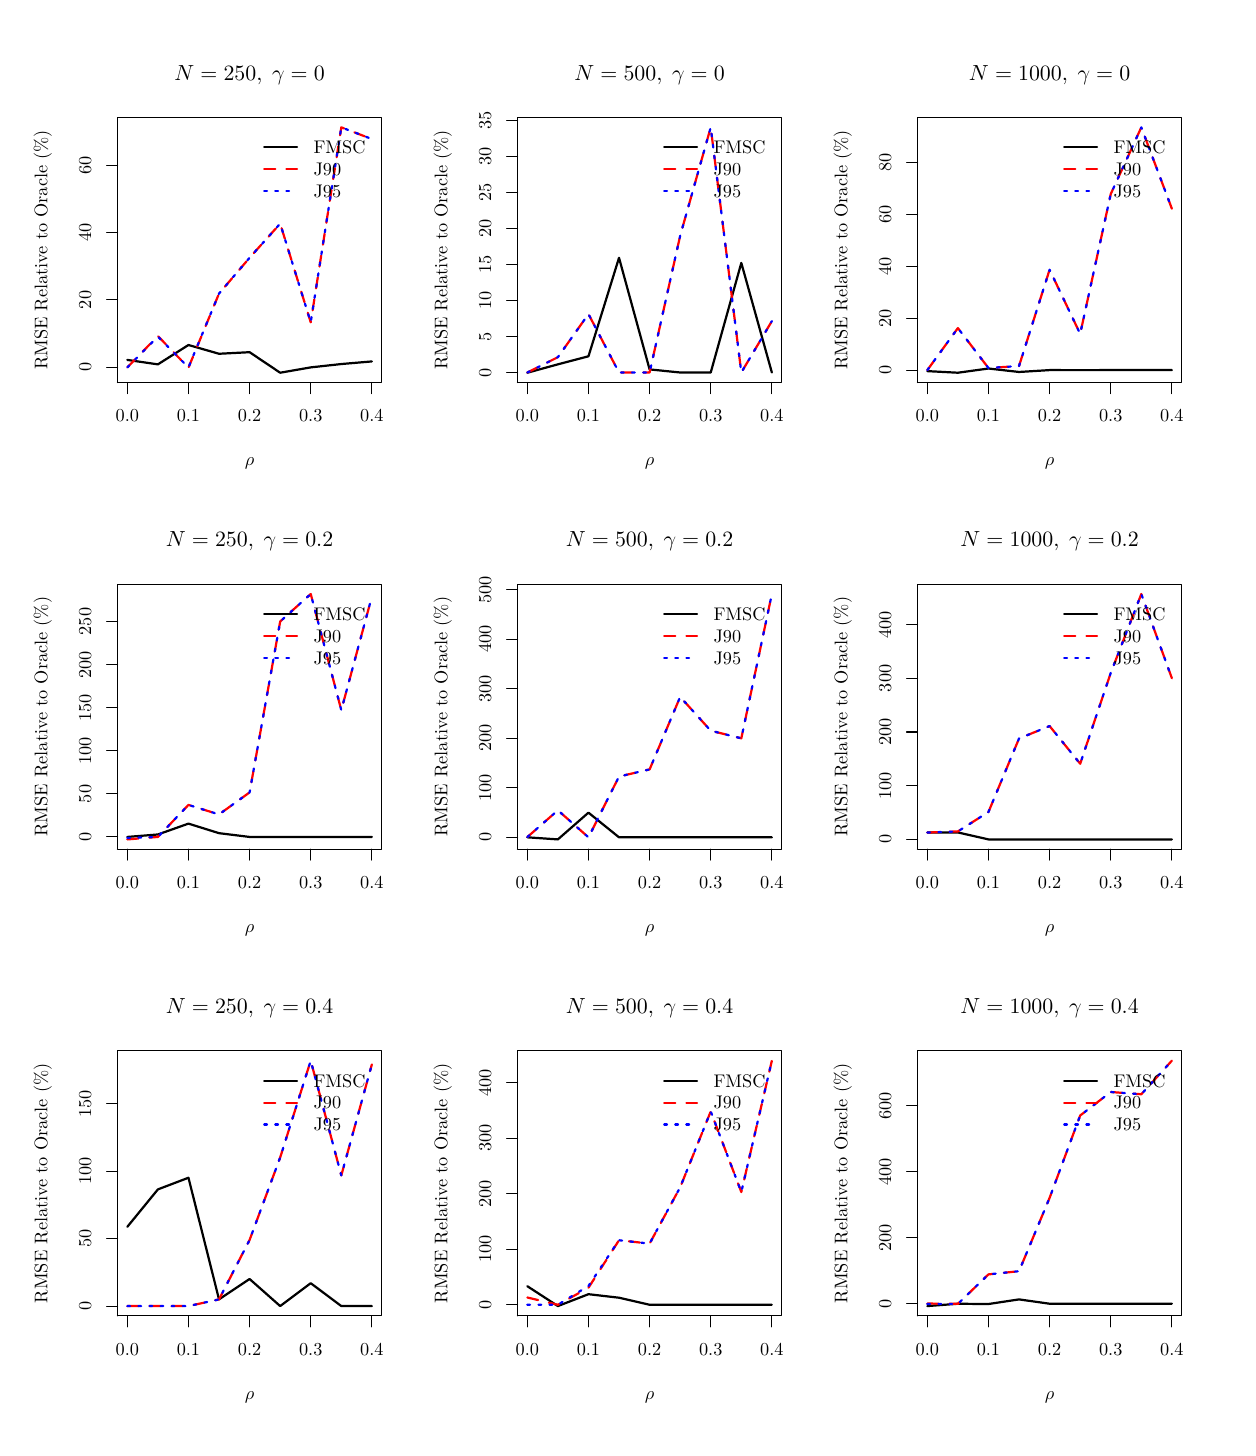
\begin{tikzpicture}[x=1pt,y=1pt]
\definecolor[named]{fillColor}{rgb}{1.00,1.00,1.00}
\path[use as bounding box,fill=fillColor,fill opacity=0.00] (0,0) rectangle (433.62,505.89);
\begin{scope}
\path[clip] ( 32.47,377.65) rectangle (127.91,473.42);
\definecolor[named]{drawColor}{rgb}{0.00,0.00,0.00}

\path[draw=drawColor,line width= 0.8pt,line join=round,line cap=round] ( 36.01,385.83) --
	( 47.05,384.22) --
	( 58.10,391.22) --
	( 69.14,388.05) --
	( 80.19,388.62) --
	( 91.24,381.20) --
	(102.28,383.13) --
	(113.33,384.34) --
	(124.37,385.28);
\end{scope}
\begin{scope}
\path[clip] (  0.00,  0.00) rectangle (433.62,505.89);
\definecolor[named]{drawColor}{rgb}{0.00,0.00,0.00}

\path[draw=drawColor,line width= 0.4pt,line join=round,line cap=round] ( 36.01,377.65) -- (124.37,377.65);

\path[draw=drawColor,line width= 0.4pt,line join=round,line cap=round] ( 36.01,377.65) -- ( 36.01,373.69);

\path[draw=drawColor,line width= 0.4pt,line join=round,line cap=round] ( 58.10,377.65) -- ( 58.10,373.69);

\path[draw=drawColor,line width= 0.4pt,line join=round,line cap=round] ( 80.19,377.65) -- ( 80.19,373.69);

\path[draw=drawColor,line width= 0.4pt,line join=round,line cap=round] (102.28,377.65) -- (102.28,373.69);

\path[draw=drawColor,line width= 0.4pt,line join=round,line cap=round] (124.37,377.65) -- (124.37,373.69);

\node[text=drawColor,anchor=base,inner sep=0pt, outer sep=0pt, scale=  0.66] at ( 36.01,363.40) {0.0};

\node[text=drawColor,anchor=base,inner sep=0pt, outer sep=0pt, scale=  0.66] at ( 58.10,363.40) {0.1};

\node[text=drawColor,anchor=base,inner sep=0pt, outer sep=0pt, scale=  0.66] at ( 80.19,363.40) {0.2};

\node[text=drawColor,anchor=base,inner sep=0pt, outer sep=0pt, scale=  0.66] at (102.28,363.40) {0.3};

\node[text=drawColor,anchor=base,inner sep=0pt, outer sep=0pt, scale=  0.66] at (124.37,363.40) {0.4};

\path[draw=drawColor,line width= 0.4pt,line join=round,line cap=round] ( 32.47,383.13) -- ( 32.47,456.23);

\path[draw=drawColor,line width= 0.4pt,line join=round,line cap=round] ( 32.47,383.13) -- ( 28.51,383.13);

\path[draw=drawColor,line width= 0.4pt,line join=round,line cap=round] ( 32.47,407.50) -- ( 28.51,407.50);

\path[draw=drawColor,line width= 0.4pt,line join=round,line cap=round] ( 32.47,431.86) -- ( 28.51,431.86);

\path[draw=drawColor,line width= 0.4pt,line join=round,line cap=round] ( 32.47,456.23) -- ( 28.51,456.23);

\node[text=drawColor,rotate= 90.00,anchor=base,inner sep=0pt, outer sep=0pt, scale=  0.66] at ( 22.97,383.13) {0};

\node[text=drawColor,rotate= 90.00,anchor=base,inner sep=0pt, outer sep=0pt, scale=  0.66] at ( 22.97,407.50) {20};

\node[text=drawColor,rotate= 90.00,anchor=base,inner sep=0pt, outer sep=0pt, scale=  0.66] at ( 22.97,431.86) {40};

\node[text=drawColor,rotate= 90.00,anchor=base,inner sep=0pt, outer sep=0pt, scale=  0.66] at ( 22.97,456.23) {60};

\path[draw=drawColor,line width= 0.4pt,line join=round,line cap=round] ( 32.47,377.65) --
	(127.91,377.65) --
	(127.91,473.42) --
	( 32.47,473.42) --
	( 32.47,377.65);
\end{scope}
\begin{scope}
\path[clip] (  0.00,337.26) rectangle (144.54,505.89);
\definecolor[named]{drawColor}{rgb}{0.00,0.00,0.00}

\node[text=drawColor,anchor=base,inner sep=0pt, outer sep=0pt, scale=  0.79] at ( 80.19,486.92) {\bfseries $N=250, \;\gamma=0$};

\node[text=drawColor,anchor=base,inner sep=0pt, outer sep=0pt, scale=  0.66] at ( 80.19,347.56) {$\rho$};

\node[text=drawColor,rotate= 90.00,anchor=base,inner sep=0pt, outer sep=0pt, scale=  0.66] at (  7.13,425.53) {RMSE Relative to Oracle (\%)};
\end{scope}
\begin{scope}
\path[clip] ( 32.47,377.65) rectangle (127.91,473.42);
\definecolor[named]{drawColor}{rgb}{1.00,0.00,0.00}

\path[draw=drawColor,line width= 0.8pt,dash pattern=on 4pt off 4pt ,line join=round,line cap=round] ( 36.01,383.13) --
	( 47.05,394.47) --
	( 58.10,383.02) --
	( 69.14,409.80) --
	( 80.19,422.75) --
	( 91.24,435.07) --
	(102.28,399.42) --
	(113.33,469.87) --
	(124.37,465.64);
\definecolor[named]{drawColor}{rgb}{0.00,0.00,1.00}

\path[draw=drawColor,line width= 0.8pt,dash pattern=on 1pt off 3pt ,line join=round,line cap=round] ( 36.01,383.13) --
	( 47.05,394.24) --
	( 58.10,383.13) --
	( 69.14,409.80) --
	( 80.19,422.75) --
	( 91.24,435.07) --
	(102.28,399.42) --
	(113.33,469.87) --
	(124.37,465.64);
\definecolor[named]{drawColor}{rgb}{0.00,0.00,0.00}

\path[draw=drawColor,line width= 0.8pt,line join=round,line cap=round] ( 85.47,462.63) -- ( 97.35,462.63);
\definecolor[named]{drawColor}{rgb}{1.00,0.00,0.00}

\path[draw=drawColor,line width= 0.8pt,dash pattern=on 4pt off 4pt ,line join=round,line cap=round] ( 85.47,454.71) -- ( 97.35,454.71);
\definecolor[named]{drawColor}{rgb}{0.00,0.00,1.00}

\path[draw=drawColor,line width= 0.8pt,dash pattern=on 1pt off 3pt ,line join=round,line cap=round] ( 85.47,446.79) -- ( 97.35,446.79);
\definecolor[named]{drawColor}{rgb}{0.00,0.00,0.00}

\node[text=drawColor,anchor=base west,inner sep=0pt, outer sep=0pt, scale=  0.66] at (103.29,460.35) {FMSC};

\node[text=drawColor,anchor=base west,inner sep=0pt, outer sep=0pt, scale=  0.66] at (103.29,452.43) {J90};

\node[text=drawColor,anchor=base west,inner sep=0pt, outer sep=0pt, scale=  0.66] at (103.29,444.51) {J95};
\end{scope}
\begin{scope}
\path[clip] (177.01,377.65) rectangle (272.45,473.42);
\definecolor[named]{drawColor}{rgb}{0.00,0.00,0.00}

\path[draw=drawColor,line width= 0.8pt,line join=round,line cap=round] (180.55,381.20) --
	(191.59,384.23) --
	(202.64,387.14) --
	(213.68,422.73) --
	(224.73,382.40) --
	(235.78,381.28) --
	(246.82,381.28) --
	(257.87,420.88) --
	(268.91,381.28);
\end{scope}
\begin{scope}
\path[clip] (  0.00,  0.00) rectangle (433.62,505.89);
\definecolor[named]{drawColor}{rgb}{0.00,0.00,0.00}

\path[draw=drawColor,line width= 0.4pt,line join=round,line cap=round] (180.55,377.65) -- (268.91,377.65);

\path[draw=drawColor,line width= 0.4pt,line join=round,line cap=round] (180.55,377.65) -- (180.55,373.69);

\path[draw=drawColor,line width= 0.4pt,line join=round,line cap=round] (202.64,377.65) -- (202.64,373.69);

\path[draw=drawColor,line width= 0.4pt,line join=round,line cap=round] (224.73,377.65) -- (224.73,373.69);

\path[draw=drawColor,line width= 0.4pt,line join=round,line cap=round] (246.82,377.65) -- (246.82,373.69);

\path[draw=drawColor,line width= 0.4pt,line join=round,line cap=round] (268.91,377.65) -- (268.91,373.69);

\node[text=drawColor,anchor=base,inner sep=0pt, outer sep=0pt, scale=  0.66] at (180.55,363.40) {0.0};

\node[text=drawColor,anchor=base,inner sep=0pt, outer sep=0pt, scale=  0.66] at (202.64,363.40) {0.1};

\node[text=drawColor,anchor=base,inner sep=0pt, outer sep=0pt, scale=  0.66] at (224.73,363.40) {0.2};

\node[text=drawColor,anchor=base,inner sep=0pt, outer sep=0pt, scale=  0.66] at (246.82,363.40) {0.3};

\node[text=drawColor,anchor=base,inner sep=0pt, outer sep=0pt, scale=  0.66] at (268.91,363.40) {0.4};

\path[draw=drawColor,line width= 0.4pt,line join=round,line cap=round] (177.01,381.28) -- (177.01,472.38);

\path[draw=drawColor,line width= 0.4pt,line join=round,line cap=round] (177.01,381.28) -- (173.05,381.28);

\path[draw=drawColor,line width= 0.4pt,line join=round,line cap=round] (177.01,394.30) -- (173.05,394.30);

\path[draw=drawColor,line width= 0.4pt,line join=round,line cap=round] (177.01,407.31) -- (173.05,407.31);

\path[draw=drawColor,line width= 0.4pt,line join=round,line cap=round] (177.01,420.32) -- (173.05,420.32);

\path[draw=drawColor,line width= 0.4pt,line join=round,line cap=round] (177.01,433.34) -- (173.05,433.34);

\path[draw=drawColor,line width= 0.4pt,line join=round,line cap=round] (177.01,446.35) -- (173.05,446.35);

\path[draw=drawColor,line width= 0.4pt,line join=round,line cap=round] (177.01,459.36) -- (173.05,459.36);

\path[draw=drawColor,line width= 0.4pt,line join=round,line cap=round] (177.01,472.38) -- (173.05,472.38);

\node[text=drawColor,rotate= 90.00,anchor=base,inner sep=0pt, outer sep=0pt, scale=  0.66] at (167.51,381.28) {0};

\node[text=drawColor,rotate= 90.00,anchor=base,inner sep=0pt, outer sep=0pt, scale=  0.66] at (167.51,394.30) {5};

\node[text=drawColor,rotate= 90.00,anchor=base,inner sep=0pt, outer sep=0pt, scale=  0.66] at (167.51,407.31) {10};

\node[text=drawColor,rotate= 90.00,anchor=base,inner sep=0pt, outer sep=0pt, scale=  0.66] at (167.51,420.32) {15};

\node[text=drawColor,rotate= 90.00,anchor=base,inner sep=0pt, outer sep=0pt, scale=  0.66] at (167.51,433.34) {20};

\node[text=drawColor,rotate= 90.00,anchor=base,inner sep=0pt, outer sep=0pt, scale=  0.66] at (167.51,446.35) {25};

\node[text=drawColor,rotate= 90.00,anchor=base,inner sep=0pt, outer sep=0pt, scale=  0.66] at (167.51,459.36) {30};

\node[text=drawColor,rotate= 90.00,anchor=base,inner sep=0pt, outer sep=0pt, scale=  0.66] at (167.51,472.38) {35};

\path[draw=drawColor,line width= 0.4pt,line join=round,line cap=round] (177.01,377.65) --
	(272.45,377.65) --
	(272.45,473.42) --
	(177.01,473.42) --
	(177.01,377.65);
\end{scope}
\begin{scope}
\path[clip] (144.54,337.26) rectangle (289.08,505.89);
\definecolor[named]{drawColor}{rgb}{0.00,0.00,0.00}

\node[text=drawColor,anchor=base,inner sep=0pt, outer sep=0pt, scale=  0.79] at (224.73,486.92) {\bfseries $N=500, \;\gamma=0$};

\node[text=drawColor,anchor=base,inner sep=0pt, outer sep=0pt, scale=  0.66] at (224.73,347.56) {$\rho$};

\node[text=drawColor,rotate= 90.00,anchor=base,inner sep=0pt, outer sep=0pt, scale=  0.66] at (151.67,425.53) {RMSE Relative to Oracle (\%)};
\end{scope}
\begin{scope}
\path[clip] (177.01,377.65) rectangle (272.45,473.42);
\definecolor[named]{drawColor}{rgb}{1.00,0.00,0.00}

\path[draw=drawColor,line width= 0.8pt,dash pattern=on 4pt off 4pt ,line join=round,line cap=round] (180.55,381.28) --
	(191.59,386.82) --
	(202.64,402.40) --
	(213.68,381.28) --
	(224.73,381.28) --
	(235.78,430.71) --
	(246.82,469.87) --
	(257.87,381.28) --
	(268.91,399.84);
\definecolor[named]{drawColor}{rgb}{0.00,0.00,1.00}

\path[draw=drawColor,line width= 0.8pt,dash pattern=on 1pt off 3pt ,line join=round,line cap=round] (180.55,381.28) --
	(191.59,386.82) --
	(202.64,402.40) --
	(213.68,381.28) --
	(224.73,381.28) --
	(235.78,430.71) --
	(246.82,469.87) --
	(257.87,381.28) --
	(268.91,399.84);
\definecolor[named]{drawColor}{rgb}{0.00,0.00,0.00}

\path[draw=drawColor,line width= 0.8pt,line join=round,line cap=round] (230.01,462.63) -- (241.89,462.63);
\definecolor[named]{drawColor}{rgb}{1.00,0.00,0.00}

\path[draw=drawColor,line width= 0.8pt,dash pattern=on 4pt off 4pt ,line join=round,line cap=round] (230.01,454.71) -- (241.89,454.71);
\definecolor[named]{drawColor}{rgb}{0.00,0.00,1.00}

\path[draw=drawColor,line width= 0.8pt,dash pattern=on 1pt off 3pt ,line join=round,line cap=round] (230.01,446.79) -- (241.89,446.79);
\definecolor[named]{drawColor}{rgb}{0.00,0.00,0.00}

\node[text=drawColor,anchor=base west,inner sep=0pt, outer sep=0pt, scale=  0.66] at (247.83,460.35) {FMSC};

\node[text=drawColor,anchor=base west,inner sep=0pt, outer sep=0pt, scale=  0.66] at (247.83,452.43) {J90};

\node[text=drawColor,anchor=base west,inner sep=0pt, outer sep=0pt, scale=  0.66] at (247.83,444.51) {J95};
\end{scope}
\begin{scope}
\path[clip] (321.55,377.65) rectangle (416.99,473.42);
\definecolor[named]{drawColor}{rgb}{0.00,0.00,0.00}

\path[draw=drawColor,line width= 0.8pt,line join=round,line cap=round] (325.09,381.78) --
	(336.13,381.20) --
	(347.18,382.72) --
	(358.22,381.47) --
	(369.27,382.15) --
	(380.32,382.14) --
	(391.36,382.15) --
	(402.41,382.15) --
	(413.45,382.15);
\end{scope}
\begin{scope}
\path[clip] (  0.00,  0.00) rectangle (433.62,505.89);
\definecolor[named]{drawColor}{rgb}{0.00,0.00,0.00}

\path[draw=drawColor,line width= 0.4pt,line join=round,line cap=round] (325.09,377.65) -- (413.45,377.65);

\path[draw=drawColor,line width= 0.4pt,line join=round,line cap=round] (325.09,377.65) -- (325.09,373.69);

\path[draw=drawColor,line width= 0.4pt,line join=round,line cap=round] (347.18,377.65) -- (347.18,373.69);

\path[draw=drawColor,line width= 0.4pt,line join=round,line cap=round] (369.27,377.65) -- (369.27,373.69);

\path[draw=drawColor,line width= 0.4pt,line join=round,line cap=round] (391.36,377.65) -- (391.36,373.69);

\path[draw=drawColor,line width= 0.4pt,line join=round,line cap=round] (413.45,377.65) -- (413.45,373.69);

\node[text=drawColor,anchor=base,inner sep=0pt, outer sep=0pt, scale=  0.66] at (325.09,363.40) {0.0};

\node[text=drawColor,anchor=base,inner sep=0pt, outer sep=0pt, scale=  0.66] at (347.18,363.40) {0.1};

\node[text=drawColor,anchor=base,inner sep=0pt, outer sep=0pt, scale=  0.66] at (369.27,363.40) {0.2};

\node[text=drawColor,anchor=base,inner sep=0pt, outer sep=0pt, scale=  0.66] at (391.36,363.40) {0.3};

\node[text=drawColor,anchor=base,inner sep=0pt, outer sep=0pt, scale=  0.66] at (413.45,363.40) {0.4};

\path[draw=drawColor,line width= 0.4pt,line join=round,line cap=round] (321.55,382.15) -- (321.55,457.24);

\path[draw=drawColor,line width= 0.4pt,line join=round,line cap=round] (321.55,382.15) -- (317.59,382.15);

\path[draw=drawColor,line width= 0.4pt,line join=round,line cap=round] (321.55,400.93) -- (317.59,400.93);

\path[draw=drawColor,line width= 0.4pt,line join=round,line cap=round] (321.55,419.70) -- (317.59,419.70);

\path[draw=drawColor,line width= 0.4pt,line join=round,line cap=round] (321.55,438.47) -- (317.59,438.47);

\path[draw=drawColor,line width= 0.4pt,line join=round,line cap=round] (321.55,457.24) -- (317.59,457.24);

\node[text=drawColor,rotate= 90.00,anchor=base,inner sep=0pt, outer sep=0pt, scale=  0.66] at (312.05,382.15) {0};

\node[text=drawColor,rotate= 90.00,anchor=base,inner sep=0pt, outer sep=0pt, scale=  0.66] at (312.05,400.93) {20};

\node[text=drawColor,rotate= 90.00,anchor=base,inner sep=0pt, outer sep=0pt, scale=  0.66] at (312.05,419.70) {40};

\node[text=drawColor,rotate= 90.00,anchor=base,inner sep=0pt, outer sep=0pt, scale=  0.66] at (312.05,438.47) {60};

\node[text=drawColor,rotate= 90.00,anchor=base,inner sep=0pt, outer sep=0pt, scale=  0.66] at (312.05,457.24) {80};

\path[draw=drawColor,line width= 0.4pt,line join=round,line cap=round] (321.55,377.65) --
	(416.99,377.65) --
	(416.99,473.42) --
	(321.55,473.42) --
	(321.55,377.65);
\end{scope}
\begin{scope}
\path[clip] (289.08,337.26) rectangle (433.62,505.89);
\definecolor[named]{drawColor}{rgb}{0.00,0.00,0.00}

\node[text=drawColor,anchor=base,inner sep=0pt, outer sep=0pt, scale=  0.79] at (369.27,486.92) {\bfseries $N=1000, \;\gamma=0$};

\node[text=drawColor,anchor=base,inner sep=0pt, outer sep=0pt, scale=  0.66] at (369.27,347.56) {$\rho$};

\node[text=drawColor,rotate= 90.00,anchor=base,inner sep=0pt, outer sep=0pt, scale=  0.66] at (296.21,425.53) {RMSE Relative to Oracle (\%)};
\end{scope}
\begin{scope}
\path[clip] (321.55,377.65) rectangle (416.99,473.42);
\definecolor[named]{drawColor}{rgb}{1.00,0.00,0.00}

\path[draw=drawColor,line width= 0.8pt,dash pattern=on 4pt off 4pt ,line join=round,line cap=round] (325.09,382.15) --
	(336.13,397.33) --
	(347.18,382.90) --
	(358.22,383.63) --
	(369.27,418.42) --
	(380.32,395.24) --
	(391.36,445.76) --
	(402.41,469.87) --
	(413.45,440.47);
\definecolor[named]{drawColor}{rgb}{0.00,0.00,1.00}

\path[draw=drawColor,line width= 0.8pt,dash pattern=on 1pt off 3pt ,line join=round,line cap=round] (325.09,382.15) --
	(336.13,397.33) --
	(347.18,382.90) --
	(358.22,383.63) --
	(369.27,418.42) --
	(380.32,395.24) --
	(391.36,445.76) --
	(402.41,469.87) --
	(413.45,440.47);
\definecolor[named]{drawColor}{rgb}{0.00,0.00,0.00}

\path[draw=drawColor,line width= 0.8pt,line join=round,line cap=round] (374.55,462.63) -- (386.43,462.63);
\definecolor[named]{drawColor}{rgb}{1.00,0.00,0.00}

\path[draw=drawColor,line width= 0.8pt,dash pattern=on 4pt off 4pt ,line join=round,line cap=round] (374.55,454.71) -- (386.43,454.71);
\definecolor[named]{drawColor}{rgb}{0.00,0.00,1.00}

\path[draw=drawColor,line width= 0.8pt,dash pattern=on 1pt off 3pt ,line join=round,line cap=round] (374.55,446.79) -- (386.43,446.79);
\definecolor[named]{drawColor}{rgb}{0.00,0.00,0.00}

\node[text=drawColor,anchor=base west,inner sep=0pt, outer sep=0pt, scale=  0.66] at (392.37,460.35) {FMSC};

\node[text=drawColor,anchor=base west,inner sep=0pt, outer sep=0pt, scale=  0.66] at (392.37,452.43) {J90};

\node[text=drawColor,anchor=base west,inner sep=0pt, outer sep=0pt, scale=  0.66] at (392.37,444.51) {J95};
\end{scope}
\begin{scope}
\path[clip] ( 32.47,209.02) rectangle (127.91,304.79);
\definecolor[named]{drawColor}{rgb}{0.00,0.00,0.00}

\path[draw=drawColor,line width= 0.8pt,line join=round,line cap=round] ( 36.01,213.46) --
	( 47.05,214.35) --
	( 58.10,218.27) --
	( 69.14,214.82) --
	( 80.19,213.46) --
	( 91.24,213.46) --
	(102.28,213.46) --
	(113.33,213.46) --
	(124.37,213.46);
\end{scope}
\begin{scope}
\path[clip] (  0.00,  0.00) rectangle (433.62,505.89);
\definecolor[named]{drawColor}{rgb}{0.00,0.00,0.00}

\path[draw=drawColor,line width= 0.4pt,line join=round,line cap=round] ( 36.01,209.02) -- (124.37,209.02);

\path[draw=drawColor,line width= 0.4pt,line join=round,line cap=round] ( 36.01,209.02) -- ( 36.01,205.06);

\path[draw=drawColor,line width= 0.4pt,line join=round,line cap=round] ( 58.10,209.02) -- ( 58.10,205.06);

\path[draw=drawColor,line width= 0.4pt,line join=round,line cap=round] ( 80.19,209.02) -- ( 80.19,205.06);

\path[draw=drawColor,line width= 0.4pt,line join=round,line cap=round] (102.28,209.02) -- (102.28,205.06);

\path[draw=drawColor,line width= 0.4pt,line join=round,line cap=round] (124.37,209.02) -- (124.37,205.06);

\node[text=drawColor,anchor=base,inner sep=0pt, outer sep=0pt, scale=  0.66] at ( 36.01,194.77) {0.0};

\node[text=drawColor,anchor=base,inner sep=0pt, outer sep=0pt, scale=  0.66] at ( 58.10,194.77) {0.1};

\node[text=drawColor,anchor=base,inner sep=0pt, outer sep=0pt, scale=  0.66] at ( 80.19,194.77) {0.2};

\node[text=drawColor,anchor=base,inner sep=0pt, outer sep=0pt, scale=  0.66] at (102.28,194.77) {0.3};

\node[text=drawColor,anchor=base,inner sep=0pt, outer sep=0pt, scale=  0.66] at (124.37,194.77) {0.4};

\path[draw=drawColor,line width= 0.4pt,line join=round,line cap=round] ( 32.47,213.46) -- ( 32.47,291.29);

\path[draw=drawColor,line width= 0.4pt,line join=round,line cap=round] ( 32.47,213.46) -- ( 28.51,213.46);

\path[draw=drawColor,line width= 0.4pt,line join=round,line cap=round] ( 32.47,229.02) -- ( 28.51,229.02);

\path[draw=drawColor,line width= 0.4pt,line join=round,line cap=round] ( 32.47,244.59) -- ( 28.51,244.59);

\path[draw=drawColor,line width= 0.4pt,line join=round,line cap=round] ( 32.47,260.16) -- ( 28.51,260.16);

\path[draw=drawColor,line width= 0.4pt,line join=round,line cap=round] ( 32.47,275.73) -- ( 28.51,275.73);

\path[draw=drawColor,line width= 0.4pt,line join=round,line cap=round] ( 32.47,291.29) -- ( 28.51,291.29);

\node[text=drawColor,rotate= 90.00,anchor=base,inner sep=0pt, outer sep=0pt, scale=  0.66] at ( 22.97,213.46) {0};

\node[text=drawColor,rotate= 90.00,anchor=base,inner sep=0pt, outer sep=0pt, scale=  0.66] at ( 22.97,229.02) {50};

\node[text=drawColor,rotate= 90.00,anchor=base,inner sep=0pt, outer sep=0pt, scale=  0.66] at ( 22.97,244.59) {100};

\node[text=drawColor,rotate= 90.00,anchor=base,inner sep=0pt, outer sep=0pt, scale=  0.66] at ( 22.97,260.16) {150};

\node[text=drawColor,rotate= 90.00,anchor=base,inner sep=0pt, outer sep=0pt, scale=  0.66] at ( 22.97,275.73) {200};

\node[text=drawColor,rotate= 90.00,anchor=base,inner sep=0pt, outer sep=0pt, scale=  0.66] at ( 22.97,291.29) {250};

\path[draw=drawColor,line width= 0.4pt,line join=round,line cap=round] ( 32.47,209.02) --
	(127.91,209.02) --
	(127.91,304.79) --
	( 32.47,304.79) --
	( 32.47,209.02);
\end{scope}
\begin{scope}
\path[clip] (  0.00,168.63) rectangle (144.54,337.26);
\definecolor[named]{drawColor}{rgb}{0.00,0.00,0.00}

\node[text=drawColor,anchor=base,inner sep=0pt, outer sep=0pt, scale=  0.79] at ( 80.19,318.29) {\bfseries $N=250, \;\gamma=0.2$};

\node[text=drawColor,anchor=base,inner sep=0pt, outer sep=0pt, scale=  0.66] at ( 80.19,178.93) {$\rho$};

\node[text=drawColor,rotate= 90.00,anchor=base,inner sep=0pt, outer sep=0pt, scale=  0.66] at (  7.13,256.90) {RMSE Relative to Oracle (\%)};
\end{scope}
\begin{scope}
\path[clip] ( 32.47,209.02) rectangle (127.91,304.79);
\definecolor[named]{drawColor}{rgb}{1.00,0.00,0.00}

\path[draw=drawColor,line width= 0.8pt,dash pattern=on 4pt off 4pt ,line join=round,line cap=round] ( 36.01,212.57) --
	( 47.05,213.46) --
	( 58.10,225.03) --
	( 69.14,221.59) --
	( 80.19,229.55) --
	( 91.24,291.31) --
	(102.28,301.24) --
	(113.33,259.28) --
	(124.37,300.30);
\definecolor[named]{drawColor}{rgb}{0.00,0.00,1.00}

\path[draw=drawColor,line width= 0.8pt,dash pattern=on 1pt off 3pt ,line join=round,line cap=round] ( 36.01,213.09) --
	( 47.05,213.46) --
	( 58.10,225.03) --
	( 69.14,221.59) --
	( 80.19,229.55) --
	( 91.24,291.31) --
	(102.28,301.24) --
	(113.33,259.28) --
	(124.37,300.30);
\definecolor[named]{drawColor}{rgb}{0.00,0.00,0.00}

\path[draw=drawColor,line width= 0.8pt,line join=round,line cap=round] ( 85.47,294.00) -- ( 97.35,294.00);
\definecolor[named]{drawColor}{rgb}{1.00,0.00,0.00}

\path[draw=drawColor,line width= 0.8pt,dash pattern=on 4pt off 4pt ,line join=round,line cap=round] ( 85.47,286.08) -- ( 97.35,286.08);
\definecolor[named]{drawColor}{rgb}{0.00,0.00,1.00}

\path[draw=drawColor,line width= 0.8pt,dash pattern=on 1pt off 3pt ,line join=round,line cap=round] ( 85.47,278.16) -- ( 97.35,278.16);
\definecolor[named]{drawColor}{rgb}{0.00,0.00,0.00}

\node[text=drawColor,anchor=base west,inner sep=0pt, outer sep=0pt, scale=  0.66] at (103.29,291.72) {FMSC};

\node[text=drawColor,anchor=base west,inner sep=0pt, outer sep=0pt, scale=  0.66] at (103.29,283.80) {J90};

\node[text=drawColor,anchor=base west,inner sep=0pt, outer sep=0pt, scale=  0.66] at (103.29,275.88) {J95};
\end{scope}
\begin{scope}
\path[clip] (177.01,209.02) rectangle (272.45,304.79);
\definecolor[named]{drawColor}{rgb}{0.00,0.00,0.00}

\path[draw=drawColor,line width= 0.8pt,line join=round,line cap=round] (180.55,213.32) --
	(191.59,212.57) --
	(202.64,222.24) --
	(213.68,213.32) --
	(224.73,213.32) --
	(235.78,213.32) --
	(246.82,213.32) --
	(257.87,213.32) --
	(268.91,213.32);
\end{scope}
\begin{scope}
\path[clip] (  0.00,  0.00) rectangle (433.62,505.89);
\definecolor[named]{drawColor}{rgb}{0.00,0.00,0.00}

\path[draw=drawColor,line width= 0.4pt,line join=round,line cap=round] (180.55,209.02) -- (268.91,209.02);

\path[draw=drawColor,line width= 0.4pt,line join=round,line cap=round] (180.55,209.02) -- (180.55,205.06);

\path[draw=drawColor,line width= 0.4pt,line join=round,line cap=round] (202.64,209.02) -- (202.64,205.06);

\path[draw=drawColor,line width= 0.4pt,line join=round,line cap=round] (224.73,209.02) -- (224.73,205.06);

\path[draw=drawColor,line width= 0.4pt,line join=round,line cap=round] (246.82,209.02) -- (246.82,205.06);

\path[draw=drawColor,line width= 0.4pt,line join=round,line cap=round] (268.91,209.02) -- (268.91,205.06);

\node[text=drawColor,anchor=base,inner sep=0pt, outer sep=0pt, scale=  0.66] at (180.55,194.77) {0.0};

\node[text=drawColor,anchor=base,inner sep=0pt, outer sep=0pt, scale=  0.66] at (202.64,194.77) {0.1};

\node[text=drawColor,anchor=base,inner sep=0pt, outer sep=0pt, scale=  0.66] at (224.73,194.77) {0.2};

\node[text=drawColor,anchor=base,inner sep=0pt, outer sep=0pt, scale=  0.66] at (246.82,194.77) {0.3};

\node[text=drawColor,anchor=base,inner sep=0pt, outer sep=0pt, scale=  0.66] at (268.91,194.77) {0.4};

\path[draw=drawColor,line width= 0.4pt,line join=round,line cap=round] (177.01,213.32) -- (177.01,302.82);

\path[draw=drawColor,line width= 0.4pt,line join=round,line cap=round] (177.01,213.32) -- (173.05,213.32);

\path[draw=drawColor,line width= 0.4pt,line join=round,line cap=round] (177.01,231.22) -- (173.05,231.22);

\path[draw=drawColor,line width= 0.4pt,line join=round,line cap=round] (177.01,249.12) -- (173.05,249.12);

\path[draw=drawColor,line width= 0.4pt,line join=round,line cap=round] (177.01,267.02) -- (173.05,267.02);

\path[draw=drawColor,line width= 0.4pt,line join=round,line cap=round] (177.01,284.92) -- (173.05,284.92);

\path[draw=drawColor,line width= 0.4pt,line join=round,line cap=round] (177.01,302.82) -- (173.05,302.82);

\node[text=drawColor,rotate= 90.00,anchor=base,inner sep=0pt, outer sep=0pt, scale=  0.66] at (167.51,213.32) {0};

\node[text=drawColor,rotate= 90.00,anchor=base,inner sep=0pt, outer sep=0pt, scale=  0.66] at (167.51,231.22) {100};

\node[text=drawColor,rotate= 90.00,anchor=base,inner sep=0pt, outer sep=0pt, scale=  0.66] at (167.51,249.12) {200};

\node[text=drawColor,rotate= 90.00,anchor=base,inner sep=0pt, outer sep=0pt, scale=  0.66] at (167.51,267.02) {300};

\node[text=drawColor,rotate= 90.00,anchor=base,inner sep=0pt, outer sep=0pt, scale=  0.66] at (167.51,284.92) {400};

\node[text=drawColor,rotate= 90.00,anchor=base,inner sep=0pt, outer sep=0pt, scale=  0.66] at (167.51,302.82) {500};

\path[draw=drawColor,line width= 0.4pt,line join=round,line cap=round] (177.01,209.02) --
	(272.45,209.02) --
	(272.45,304.79) --
	(177.01,304.79) --
	(177.01,209.02);
\end{scope}
\begin{scope}
\path[clip] (144.54,168.63) rectangle (289.08,337.26);
\definecolor[named]{drawColor}{rgb}{0.00,0.00,0.00}

\node[text=drawColor,anchor=base,inner sep=0pt, outer sep=0pt, scale=  0.79] at (224.73,318.29) {\bfseries $N=500, \;\gamma=0.2$};

\node[text=drawColor,anchor=base,inner sep=0pt, outer sep=0pt, scale=  0.66] at (224.73,178.93) {$\rho$};

\node[text=drawColor,rotate= 90.00,anchor=base,inner sep=0pt, outer sep=0pt, scale=  0.66] at (151.67,256.90) {RMSE Relative to Oracle (\%)};
\end{scope}
\begin{scope}
\path[clip] (177.01,209.02) rectangle (272.45,304.79);
\definecolor[named]{drawColor}{rgb}{1.00,0.00,0.00}

\path[draw=drawColor,line width= 0.8pt,dash pattern=on 4pt off 4pt ,line join=round,line cap=round] (180.55,213.41) --
	(191.59,223.09) --
	(202.64,213.32) --
	(213.68,235.29) --
	(224.73,237.86) --
	(235.78,264.07) --
	(246.82,251.85) --
	(257.87,249.09) --
	(268.91,301.24);
\definecolor[named]{drawColor}{rgb}{0.00,0.00,1.00}

\path[draw=drawColor,line width= 0.8pt,dash pattern=on 1pt off 3pt ,line join=round,line cap=round] (180.55,213.41) --
	(191.59,223.09) --
	(202.64,213.32) --
	(213.68,235.29) --
	(224.73,237.86) --
	(235.78,264.07) --
	(246.82,251.85) --
	(257.87,249.09) --
	(268.91,301.24);
\definecolor[named]{drawColor}{rgb}{0.00,0.00,0.00}

\path[draw=drawColor,line width= 0.8pt,line join=round,line cap=round] (230.01,294.00) -- (241.89,294.00);
\definecolor[named]{drawColor}{rgb}{1.00,0.00,0.00}

\path[draw=drawColor,line width= 0.8pt,dash pattern=on 4pt off 4pt ,line join=round,line cap=round] (230.01,286.08) -- (241.89,286.08);
\definecolor[named]{drawColor}{rgb}{0.00,0.00,1.00}

\path[draw=drawColor,line width= 0.8pt,dash pattern=on 1pt off 3pt ,line join=round,line cap=round] (230.01,278.16) -- (241.89,278.16);
\definecolor[named]{drawColor}{rgb}{0.00,0.00,0.00}

\node[text=drawColor,anchor=base west,inner sep=0pt, outer sep=0pt, scale=  0.66] at (247.83,291.72) {FMSC};

\node[text=drawColor,anchor=base west,inner sep=0pt, outer sep=0pt, scale=  0.66] at (247.83,283.80) {J90};

\node[text=drawColor,anchor=base west,inner sep=0pt, outer sep=0pt, scale=  0.66] at (247.83,275.88) {J95};
\end{scope}
\begin{scope}
\path[clip] (321.55,209.02) rectangle (416.99,304.79);
\definecolor[named]{drawColor}{rgb}{0.00,0.00,0.00}

\path[draw=drawColor,line width= 0.8pt,line join=round,line cap=round] (325.09,215.10) --
	(336.13,215.08) --
	(347.18,212.57) --
	(358.22,212.57) --
	(369.27,212.57) --
	(380.32,212.57) --
	(391.36,212.57) --
	(402.41,212.57) --
	(413.45,212.57);
\end{scope}
\begin{scope}
\path[clip] (  0.00,  0.00) rectangle (433.62,505.89);
\definecolor[named]{drawColor}{rgb}{0.00,0.00,0.00}

\path[draw=drawColor,line width= 0.4pt,line join=round,line cap=round] (325.09,209.02) -- (413.45,209.02);

\path[draw=drawColor,line width= 0.4pt,line join=round,line cap=round] (325.09,209.02) -- (325.09,205.06);

\path[draw=drawColor,line width= 0.4pt,line join=round,line cap=round] (347.18,209.02) -- (347.18,205.06);

\path[draw=drawColor,line width= 0.4pt,line join=round,line cap=round] (369.27,209.02) -- (369.27,205.06);

\path[draw=drawColor,line width= 0.4pt,line join=round,line cap=round] (391.36,209.02) -- (391.36,205.06);

\path[draw=drawColor,line width= 0.4pt,line join=round,line cap=round] (413.45,209.02) -- (413.45,205.06);

\node[text=drawColor,anchor=base,inner sep=0pt, outer sep=0pt, scale=  0.66] at (325.09,194.77) {0.0};

\node[text=drawColor,anchor=base,inner sep=0pt, outer sep=0pt, scale=  0.66] at (347.18,194.77) {0.1};

\node[text=drawColor,anchor=base,inner sep=0pt, outer sep=0pt, scale=  0.66] at (369.27,194.77) {0.2};

\node[text=drawColor,anchor=base,inner sep=0pt, outer sep=0pt, scale=  0.66] at (391.36,194.77) {0.3};

\node[text=drawColor,anchor=base,inner sep=0pt, outer sep=0pt, scale=  0.66] at (413.45,194.77) {0.4};

\path[draw=drawColor,line width= 0.4pt,line join=round,line cap=round] (321.55,212.57) -- (321.55,290.15);

\path[draw=drawColor,line width= 0.4pt,line join=round,line cap=round] (321.55,212.57) -- (317.59,212.57);

\path[draw=drawColor,line width= 0.4pt,line join=round,line cap=round] (321.55,231.96) -- (317.59,231.96);

\path[draw=drawColor,line width= 0.4pt,line join=round,line cap=round] (321.55,251.36) -- (317.59,251.36);

\path[draw=drawColor,line width= 0.4pt,line join=round,line cap=round] (321.55,270.75) -- (317.59,270.75);

\path[draw=drawColor,line width= 0.4pt,line join=round,line cap=round] (321.55,290.15) -- (317.59,290.15);

\node[text=drawColor,rotate= 90.00,anchor=base,inner sep=0pt, outer sep=0pt, scale=  0.66] at (312.05,212.57) {0};

\node[text=drawColor,rotate= 90.00,anchor=base,inner sep=0pt, outer sep=0pt, scale=  0.66] at (312.05,231.96) {100};

\node[text=drawColor,rotate= 90.00,anchor=base,inner sep=0pt, outer sep=0pt, scale=  0.66] at (312.05,251.36) {200};

\node[text=drawColor,rotate= 90.00,anchor=base,inner sep=0pt, outer sep=0pt, scale=  0.66] at (312.05,270.75) {300};

\node[text=drawColor,rotate= 90.00,anchor=base,inner sep=0pt, outer sep=0pt, scale=  0.66] at (312.05,290.15) {400};

\path[draw=drawColor,line width= 0.4pt,line join=round,line cap=round] (321.55,209.02) --
	(416.99,209.02) --
	(416.99,304.79) --
	(321.55,304.79) --
	(321.55,209.02);
\end{scope}
\begin{scope}
\path[clip] (289.08,168.63) rectangle (433.62,337.26);
\definecolor[named]{drawColor}{rgb}{0.00,0.00,0.00}

\node[text=drawColor,anchor=base,inner sep=0pt, outer sep=0pt, scale=  0.79] at (369.27,318.29) {\bfseries $N=1000, \;\gamma=0.2$};

\node[text=drawColor,anchor=base,inner sep=0pt, outer sep=0pt, scale=  0.66] at (369.27,178.93) {$\rho$};

\node[text=drawColor,rotate= 90.00,anchor=base,inner sep=0pt, outer sep=0pt, scale=  0.66] at (296.21,256.90) {RMSE Relative to Oracle (\%)};
\end{scope}
\begin{scope}
\path[clip] (321.55,209.02) rectangle (416.99,304.79);
\definecolor[named]{drawColor}{rgb}{1.00,0.00,0.00}

\path[draw=drawColor,line width= 0.8pt,dash pattern=on 4pt off 4pt ,line join=round,line cap=round] (325.09,215.04) --
	(336.13,215.46) --
	(347.18,222.48) --
	(358.22,249.02) --
	(369.27,253.52) --
	(380.32,239.91) --
	(391.36,272.72) --
	(402.41,301.24) --
	(413.45,270.81);
\definecolor[named]{drawColor}{rgb}{0.00,0.00,1.00}

\path[draw=drawColor,line width= 0.8pt,dash pattern=on 1pt off 3pt ,line join=round,line cap=round] (325.09,215.04) --
	(336.13,215.46) --
	(347.18,222.48) --
	(358.22,249.02) --
	(369.27,253.52) --
	(380.32,239.91) --
	(391.36,272.72) --
	(402.41,301.24) --
	(413.45,270.81);
\definecolor[named]{drawColor}{rgb}{0.00,0.00,0.00}

\path[draw=drawColor,line width= 0.8pt,line join=round,line cap=round] (374.55,294.00) -- (386.43,294.00);
\definecolor[named]{drawColor}{rgb}{1.00,0.00,0.00}

\path[draw=drawColor,line width= 0.8pt,dash pattern=on 4pt off 4pt ,line join=round,line cap=round] (374.55,286.08) -- (386.43,286.08);
\definecolor[named]{drawColor}{rgb}{0.00,0.00,1.00}

\path[draw=drawColor,line width= 0.8pt,dash pattern=on 1pt off 3pt ,line join=round,line cap=round] (374.55,278.16) -- (386.43,278.16);
\definecolor[named]{drawColor}{rgb}{0.00,0.00,0.00}

\node[text=drawColor,anchor=base west,inner sep=0pt, outer sep=0pt, scale=  0.66] at (392.37,291.72) {FMSC};

\node[text=drawColor,anchor=base west,inner sep=0pt, outer sep=0pt, scale=  0.66] at (392.37,283.80) {J90};

\node[text=drawColor,anchor=base west,inner sep=0pt, outer sep=0pt, scale=  0.66] at (392.37,275.88) {J95};
\end{scope}
\begin{scope}
\path[clip] ( 32.47, 40.39) rectangle (127.91,136.16);
\definecolor[named]{drawColor}{rgb}{0.00,0.00,0.00}

\path[draw=drawColor,line width= 0.8pt,line join=round,line cap=round] ( 36.01, 72.58) --
	( 47.05, 86.10) --
	( 58.10, 90.31) --
	( 69.14, 46.36) --
	( 80.19, 53.72) --
	( 91.24, 43.94) --
	(102.28, 52.21) --
	(113.33, 43.94) --
	(124.37, 43.94);
\end{scope}
\begin{scope}
\path[clip] (  0.00,  0.00) rectangle (433.62,505.89);
\definecolor[named]{drawColor}{rgb}{0.00,0.00,0.00}

\path[draw=drawColor,line width= 0.4pt,line join=round,line cap=round] ( 36.01, 40.39) -- (124.37, 40.39);

\path[draw=drawColor,line width= 0.4pt,line join=round,line cap=round] ( 36.01, 40.39) -- ( 36.01, 36.43);

\path[draw=drawColor,line width= 0.4pt,line join=round,line cap=round] ( 58.10, 40.39) -- ( 58.10, 36.43);

\path[draw=drawColor,line width= 0.4pt,line join=round,line cap=round] ( 80.19, 40.39) -- ( 80.19, 36.43);

\path[draw=drawColor,line width= 0.4pt,line join=round,line cap=round] (102.28, 40.39) -- (102.28, 36.43);

\path[draw=drawColor,line width= 0.4pt,line join=round,line cap=round] (124.37, 40.39) -- (124.37, 36.43);

\node[text=drawColor,anchor=base,inner sep=0pt, outer sep=0pt, scale=  0.66] at ( 36.01, 26.14) {0.0};

\node[text=drawColor,anchor=base,inner sep=0pt, outer sep=0pt, scale=  0.66] at ( 58.10, 26.14) {0.1};

\node[text=drawColor,anchor=base,inner sep=0pt, outer sep=0pt, scale=  0.66] at ( 80.19, 26.14) {0.2};

\node[text=drawColor,anchor=base,inner sep=0pt, outer sep=0pt, scale=  0.66] at (102.28, 26.14) {0.3};

\node[text=drawColor,anchor=base,inner sep=0pt, outer sep=0pt, scale=  0.66] at (124.37, 26.14) {0.4};

\path[draw=drawColor,line width= 0.4pt,line join=round,line cap=round] ( 32.47, 43.94) -- ( 32.47,117.08);

\path[draw=drawColor,line width= 0.4pt,line join=round,line cap=round] ( 32.47, 43.94) -- ( 28.51, 43.94);

\path[draw=drawColor,line width= 0.4pt,line join=round,line cap=round] ( 32.47, 68.32) -- ( 28.51, 68.32);

\path[draw=drawColor,line width= 0.4pt,line join=round,line cap=round] ( 32.47, 92.70) -- ( 28.51, 92.70);

\path[draw=drawColor,line width= 0.4pt,line join=round,line cap=round] ( 32.47,117.08) -- ( 28.51,117.08);

\node[text=drawColor,rotate= 90.00,anchor=base,inner sep=0pt, outer sep=0pt, scale=  0.66] at ( 22.97, 43.94) {0};

\node[text=drawColor,rotate= 90.00,anchor=base,inner sep=0pt, outer sep=0pt, scale=  0.66] at ( 22.97, 68.32) {50};

\node[text=drawColor,rotate= 90.00,anchor=base,inner sep=0pt, outer sep=0pt, scale=  0.66] at ( 22.97, 92.70) {100};

\node[text=drawColor,rotate= 90.00,anchor=base,inner sep=0pt, outer sep=0pt, scale=  0.66] at ( 22.97,117.08) {150};

\path[draw=drawColor,line width= 0.4pt,line join=round,line cap=round] ( 32.47, 40.39) --
	(127.91, 40.39) --
	(127.91,136.16) --
	( 32.47,136.16) --
	( 32.47, 40.39);
\end{scope}
\begin{scope}
\path[clip] (  0.00,  0.00) rectangle (144.54,168.63);
\definecolor[named]{drawColor}{rgb}{0.00,0.00,0.00}

\node[text=drawColor,anchor=base,inner sep=0pt, outer sep=0pt, scale=  0.79] at ( 80.19,149.66) {\bfseries $N=250, \;\gamma=0.4$};

\node[text=drawColor,anchor=base,inner sep=0pt, outer sep=0pt, scale=  0.66] at ( 80.19, 10.30) {$\rho$};

\node[text=drawColor,rotate= 90.00,anchor=base,inner sep=0pt, outer sep=0pt, scale=  0.66] at (  7.13, 88.27) {RMSE Relative to Oracle (\%)};
\end{scope}
\begin{scope}
\path[clip] ( 32.47, 40.39) rectangle (127.91,136.16);
\definecolor[named]{drawColor}{rgb}{1.00,0.00,0.00}

\path[draw=drawColor,line width= 0.8pt,dash pattern=on 4pt off 4pt ,line join=round,line cap=round] ( 36.01, 43.94) --
	( 47.05, 43.94) --
	( 58.10, 43.94) --
	( 69.14, 46.35) --
	( 80.19, 67.84) --
	( 91.24, 97.63) --
	(102.28,132.61) --
	(113.33, 91.16) --
	(124.37,131.25);
\definecolor[named]{drawColor}{rgb}{0.00,0.00,1.00}

\path[draw=drawColor,line width= 0.8pt,dash pattern=on 1pt off 3pt ,line join=round,line cap=round] ( 36.01, 43.94) --
	( 47.05, 43.94) --
	( 58.10, 43.94) --
	( 69.14, 46.35) --
	( 80.19, 67.84) --
	( 91.24, 97.63) --
	(102.28,132.61) --
	(113.33, 91.16) --
	(124.37,131.25);
\definecolor[named]{drawColor}{rgb}{0.00,0.00,0.00}

\path[draw=drawColor,line width= 0.8pt,line join=round,line cap=round] ( 85.47,125.37) -- ( 97.35,125.37);
\definecolor[named]{drawColor}{rgb}{1.00,0.00,0.00}

\path[draw=drawColor,line width= 0.8pt,dash pattern=on 4pt off 4pt ,line join=round,line cap=round] ( 85.47,117.45) -- ( 97.35,117.45);
\definecolor[named]{drawColor}{rgb}{0.00,0.00,1.00}

\path[draw=drawColor,line width= 0.8pt,dash pattern=on 1pt off 3pt ,line join=round,line cap=round] ( 85.47,109.53) -- ( 97.35,109.53);
\definecolor[named]{drawColor}{rgb}{0.00,0.00,0.00}

\node[text=drawColor,anchor=base west,inner sep=0pt, outer sep=0pt, scale=  0.66] at (103.29,123.09) {FMSC};

\node[text=drawColor,anchor=base west,inner sep=0pt, outer sep=0pt, scale=  0.66] at (103.29,115.17) {J90};

\node[text=drawColor,anchor=base west,inner sep=0pt, outer sep=0pt, scale=  0.66] at (103.29,107.25) {J95};
\end{scope}
\begin{scope}
\path[clip] (177.01, 40.39) rectangle (272.45,136.16);
\definecolor[named]{drawColor}{rgb}{0.00,0.00,0.00}

\path[draw=drawColor,line width= 0.8pt,line join=round,line cap=round] (180.55, 51.12) --
	(191.59, 43.94) --
	(202.64, 48.23) --
	(213.68, 46.96) --
	(224.73, 44.41) --
	(235.78, 44.41) --
	(246.82, 44.41) --
	(257.87, 44.41) --
	(268.91, 44.41);
\end{scope}
\begin{scope}
\path[clip] (  0.00,  0.00) rectangle (433.62,505.89);
\definecolor[named]{drawColor}{rgb}{0.00,0.00,0.00}

\path[draw=drawColor,line width= 0.4pt,line join=round,line cap=round] (180.55, 40.39) -- (268.91, 40.39);

\path[draw=drawColor,line width= 0.4pt,line join=round,line cap=round] (180.55, 40.39) -- (180.55, 36.43);

\path[draw=drawColor,line width= 0.4pt,line join=round,line cap=round] (202.64, 40.39) -- (202.64, 36.43);

\path[draw=drawColor,line width= 0.4pt,line join=round,line cap=round] (224.73, 40.39) -- (224.73, 36.43);

\path[draw=drawColor,line width= 0.4pt,line join=round,line cap=round] (246.82, 40.39) -- (246.82, 36.43);

\path[draw=drawColor,line width= 0.4pt,line join=round,line cap=round] (268.91, 40.39) -- (268.91, 36.43);

\node[text=drawColor,anchor=base,inner sep=0pt, outer sep=0pt, scale=  0.66] at (180.55, 26.14) {0.0};

\node[text=drawColor,anchor=base,inner sep=0pt, outer sep=0pt, scale=  0.66] at (202.64, 26.14) {0.1};

\node[text=drawColor,anchor=base,inner sep=0pt, outer sep=0pt, scale=  0.66] at (224.73, 26.14) {0.2};

\node[text=drawColor,anchor=base,inner sep=0pt, outer sep=0pt, scale=  0.66] at (246.82, 26.14) {0.3};

\node[text=drawColor,anchor=base,inner sep=0pt, outer sep=0pt, scale=  0.66] at (268.91, 26.14) {0.4};

\path[draw=drawColor,line width= 0.4pt,line join=round,line cap=round] (177.01, 44.41) -- (177.01,124.63);

\path[draw=drawColor,line width= 0.4pt,line join=round,line cap=round] (177.01, 44.41) -- (173.05, 44.41);

\path[draw=drawColor,line width= 0.4pt,line join=round,line cap=round] (177.01, 64.46) -- (173.05, 64.46);

\path[draw=drawColor,line width= 0.4pt,line join=round,line cap=round] (177.01, 84.52) -- (173.05, 84.52);

\path[draw=drawColor,line width= 0.4pt,line join=round,line cap=round] (177.01,104.58) -- (173.05,104.58);

\path[draw=drawColor,line width= 0.4pt,line join=round,line cap=round] (177.01,124.63) -- (173.05,124.63);

\node[text=drawColor,rotate= 90.00,anchor=base,inner sep=0pt, outer sep=0pt, scale=  0.66] at (167.51, 44.41) {0};

\node[text=drawColor,rotate= 90.00,anchor=base,inner sep=0pt, outer sep=0pt, scale=  0.66] at (167.51, 64.46) {100};

\node[text=drawColor,rotate= 90.00,anchor=base,inner sep=0pt, outer sep=0pt, scale=  0.66] at (167.51, 84.52) {200};

\node[text=drawColor,rotate= 90.00,anchor=base,inner sep=0pt, outer sep=0pt, scale=  0.66] at (167.51,104.58) {300};

\node[text=drawColor,rotate= 90.00,anchor=base,inner sep=0pt, outer sep=0pt, scale=  0.66] at (167.51,124.63) {400};

\path[draw=drawColor,line width= 0.4pt,line join=round,line cap=round] (177.01, 40.39) --
	(272.45, 40.39) --
	(272.45,136.16) --
	(177.01,136.16) --
	(177.01, 40.39);
\end{scope}
\begin{scope}
\path[clip] (144.54,  0.00) rectangle (289.08,168.63);
\definecolor[named]{drawColor}{rgb}{0.00,0.00,0.00}

\node[text=drawColor,anchor=base,inner sep=0pt, outer sep=0pt, scale=  0.79] at (224.73,149.66) {\bfseries $N=500, \;\gamma=0.4$};

\node[text=drawColor,anchor=base,inner sep=0pt, outer sep=0pt, scale=  0.66] at (224.73, 10.30) {$\rho$};

\node[text=drawColor,rotate= 90.00,anchor=base,inner sep=0pt, outer sep=0pt, scale=  0.66] at (151.67, 88.27) {RMSE Relative to Oracle (\%)};
\end{scope}
\begin{scope}
\path[clip] (177.01, 40.39) rectangle (272.45,136.16);
\definecolor[named]{drawColor}{rgb}{1.00,0.00,0.00}

\path[draw=drawColor,line width= 0.8pt,dash pattern=on 4pt off 4pt ,line join=round,line cap=round] (180.55, 47.04) --
	(191.59, 44.41) --
	(202.64, 50.56) --
	(213.68, 67.73) --
	(224.73, 66.51) --
	(235.78, 86.87) --
	(246.82,114.26) --
	(257.87, 85.15) --
	(268.91,132.61);
\definecolor[named]{drawColor}{rgb}{0.00,0.00,1.00}

\path[draw=drawColor,line width= 0.8pt,dash pattern=on 1pt off 3pt ,line join=round,line cap=round] (180.55, 44.41) --
	(191.59, 44.41) --
	(202.64, 51.22) --
	(213.68, 67.73) --
	(224.73, 66.51) --
	(235.78, 86.87) --
	(246.82,114.26) --
	(257.87, 85.15) --
	(268.91,132.61);
\definecolor[named]{drawColor}{rgb}{0.00,0.00,0.00}

\path[draw=drawColor,line width= 0.8pt,line join=round,line cap=round] (230.01,125.37) -- (241.89,125.37);
\definecolor[named]{drawColor}{rgb}{1.00,0.00,0.00}

\path[draw=drawColor,line width= 0.8pt,dash pattern=on 4pt off 4pt ,line join=round,line cap=round] (230.01,117.45) -- (241.89,117.45);
\definecolor[named]{drawColor}{rgb}{0.00,0.00,1.00}

\path[draw=drawColor,line width= 0.8pt,dash pattern=on 1pt off 3pt ,line join=round,line cap=round] (230.01,109.53) -- (241.89,109.53);
\definecolor[named]{drawColor}{rgb}{0.00,0.00,0.00}

\node[text=drawColor,anchor=base west,inner sep=0pt, outer sep=0pt, scale=  0.66] at (247.83,123.09) {FMSC};

\node[text=drawColor,anchor=base west,inner sep=0pt, outer sep=0pt, scale=  0.66] at (247.83,115.17) {J90};

\node[text=drawColor,anchor=base west,inner sep=0pt, outer sep=0pt, scale=  0.66] at (247.83,107.25) {J95};
\end{scope}
\begin{scope}
\path[clip] (321.55, 40.39) rectangle (416.99,136.16);
\definecolor[named]{drawColor}{rgb}{0.00,0.00,0.00}

\path[draw=drawColor,line width= 0.8pt,line join=round,line cap=round] (325.09, 43.94) --
	(336.13, 44.77) --
	(347.18, 44.68) --
	(358.22, 46.35) --
	(369.27, 44.79) --
	(380.32, 44.79) --
	(391.36, 44.79) --
	(402.41, 44.79) --
	(413.45, 44.79);
\end{scope}
\begin{scope}
\path[clip] (  0.00,  0.00) rectangle (433.62,505.89);
\definecolor[named]{drawColor}{rgb}{0.00,0.00,0.00}

\path[draw=drawColor,line width= 0.4pt,line join=round,line cap=round] (325.09, 40.39) -- (413.45, 40.39);

\path[draw=drawColor,line width= 0.4pt,line join=round,line cap=round] (325.09, 40.39) -- (325.09, 36.43);

\path[draw=drawColor,line width= 0.4pt,line join=round,line cap=round] (347.18, 40.39) -- (347.18, 36.43);

\path[draw=drawColor,line width= 0.4pt,line join=round,line cap=round] (369.27, 40.39) -- (369.27, 36.43);

\path[draw=drawColor,line width= 0.4pt,line join=round,line cap=round] (391.36, 40.39) -- (391.36, 36.43);

\path[draw=drawColor,line width= 0.4pt,line join=round,line cap=round] (413.45, 40.39) -- (413.45, 36.43);

\node[text=drawColor,anchor=base,inner sep=0pt, outer sep=0pt, scale=  0.66] at (325.09, 26.14) {0.0};

\node[text=drawColor,anchor=base,inner sep=0pt, outer sep=0pt, scale=  0.66] at (347.18, 26.14) {0.1};

\node[text=drawColor,anchor=base,inner sep=0pt, outer sep=0pt, scale=  0.66] at (369.27, 26.14) {0.2};

\node[text=drawColor,anchor=base,inner sep=0pt, outer sep=0pt, scale=  0.66] at (391.36, 26.14) {0.3};

\node[text=drawColor,anchor=base,inner sep=0pt, outer sep=0pt, scale=  0.66] at (413.45, 26.14) {0.4};

\path[draw=drawColor,line width= 0.4pt,line join=round,line cap=round] (321.55, 44.79) -- (321.55,116.37);

\path[draw=drawColor,line width= 0.4pt,line join=round,line cap=round] (321.55, 44.79) -- (317.59, 44.79);

\path[draw=drawColor,line width= 0.4pt,line join=round,line cap=round] (321.55, 68.65) -- (317.59, 68.65);

\path[draw=drawColor,line width= 0.4pt,line join=round,line cap=round] (321.55, 92.51) -- (317.59, 92.51);

\path[draw=drawColor,line width= 0.4pt,line join=round,line cap=round] (321.55,116.37) -- (317.59,116.37);

\node[text=drawColor,rotate= 90.00,anchor=base,inner sep=0pt, outer sep=0pt, scale=  0.66] at (312.05, 44.79) {0};

\node[text=drawColor,rotate= 90.00,anchor=base,inner sep=0pt, outer sep=0pt, scale=  0.66] at (312.05, 68.65) {200};

\node[text=drawColor,rotate= 90.00,anchor=base,inner sep=0pt, outer sep=0pt, scale=  0.66] at (312.05, 92.51) {400};

\node[text=drawColor,rotate= 90.00,anchor=base,inner sep=0pt, outer sep=0pt, scale=  0.66] at (312.05,116.37) {600};

\path[draw=drawColor,line width= 0.4pt,line join=round,line cap=round] (321.55, 40.39) --
	(416.99, 40.39) --
	(416.99,136.16) --
	(321.55,136.16) --
	(321.55, 40.39);
\end{scope}
\begin{scope}
\path[clip] (289.08,  0.00) rectangle (433.62,168.63);
\definecolor[named]{drawColor}{rgb}{0.00,0.00,0.00}

\node[text=drawColor,anchor=base,inner sep=0pt, outer sep=0pt, scale=  0.79] at (369.27,149.66) {\bfseries $N=1000, \;\gamma=0.4$};

\node[text=drawColor,anchor=base,inner sep=0pt, outer sep=0pt, scale=  0.66] at (369.27, 10.30) {$\rho$};

\node[text=drawColor,rotate= 90.00,anchor=base,inner sep=0pt, outer sep=0pt, scale=  0.66] at (296.21, 88.27) {RMSE Relative to Oracle (\%)};
\end{scope}
\begin{scope}
\path[clip] (321.55, 40.39) rectangle (416.99,136.16);
\definecolor[named]{drawColor}{rgb}{1.00,0.00,0.00}

\path[draw=drawColor,line width= 0.8pt,dash pattern=on 4pt off 4pt ,line join=round,line cap=round] (325.09, 44.85) --
	(336.13, 44.74) --
	(347.18, 55.39) --
	(358.22, 56.54) --
	(369.27, 83.04) --
	(380.32,112.80) --
	(391.36,121.29) --
	(402.41,120.48) --
	(413.45,132.61);
\definecolor[named]{drawColor}{rgb}{0.00,0.00,1.00}

\path[draw=drawColor,line width= 0.8pt,dash pattern=on 1pt off 3pt ,line join=round,line cap=round] (325.09, 44.69) --
	(336.13, 44.74) --
	(347.18, 55.39) --
	(358.22, 56.54) --
	(369.27, 83.04) --
	(380.32,112.80) --
	(391.36,121.29) --
	(402.41,120.48) --
	(413.45,132.61);
\definecolor[named]{drawColor}{rgb}{0.00,0.00,0.00}

\path[draw=drawColor,line width= 0.8pt,line join=round,line cap=round] (374.55,125.37) -- (386.43,125.37);
\definecolor[named]{drawColor}{rgb}{1.00,0.00,0.00}

\path[draw=drawColor,line width= 0.8pt,dash pattern=on 4pt off 4pt ,line join=round,line cap=round] (374.55,117.45) -- (386.43,117.45);
\definecolor[named]{drawColor}{rgb}{0.00,0.00,1.00}

\path[draw=drawColor,line width= 0.8pt,dash pattern=on 1pt off 3pt ,line join=round,line cap=round] (374.55,109.53) -- (386.43,109.53);
\definecolor[named]{drawColor}{rgb}{0.00,0.00,0.00}

\node[text=drawColor,anchor=base west,inner sep=0pt, outer sep=0pt, scale=  0.66] at (392.37,123.09) {FMSC};

\node[text=drawColor,anchor=base west,inner sep=0pt, outer sep=0pt, scale=  0.66] at (392.37,115.17) {J90};

\node[text=drawColor,anchor=base west,inner sep=0pt, outer sep=0pt, scale=  0.66] at (392.37,107.25) {J95};
\end{scope}
\end{tikzpicture}

	\caption{RMSE values for the post-Focused Moment Selection Criterion (FMSC) estimator and the downward $J$-test estimator with $\alpha = 0.1$ (J90) and $\alpha = 0.05$ (J95) based on 20,000 simulation draws from the DGP given in Equations \ref{eq:chooseIVDGP1}--\ref{eq:chooseIVDGP3} using the formulas from Sections \ref{sec:chooseIVexample}.}
	\label{fig:chooseIVsim_RMSErelJ}
\end{figure}
These results are broadly similar to those for the GMM moment selection criteria of \cite{Andrews1999} considered in Section \ref{sec:chooseIVsim}, which should not come as a surprise since the J-test statistic is an ingredient in the construction of the GMM-AIC, BIC and HQ. 

\subsection{Canonical Correlations Information Criterion}
\label{sec:CCIC}
Because the GMM moment selection criteria suggested by \cite{Andrews1999} consider only instrument exogeneity, not relevance, \cite{HallPeixe2003} suggest combining them with their canonical correlations information criterion (CCIC), which aims to detect and eliminate ``redundant instruments.''
Including such instruments, which add no information beyond that already contained in the other instruments, can lead to poor finite-sample performance in spite of the fact that the first-order limit distribution is unchanged.
For the choosing instrumental variables simulation example, presented in Section \ref{sec:chooseIVsim}, the CCIC takes the following simple form
	\begin{equation}
	\mbox{CCIC}(S) = n \log\left[1 - R_n^2(S) \right] + h(p + |S|)\kappa_n
	\end{equation}
where $R_n^2(S)$ is the first-stage $R^2$ based on instrument set $S$ and $h(p + |S|)\kappa_n$ is a penalty term \citep{Jana2005}. 
Instruments are chosen to \emph{minimize} this criterion.
If we define $h(p + |S|) = (p + |S| - r)$, setting $\kappa_n = \log{n}$ gives the CCIC-BIC, while $\kappa_n = 2.01 \log{\log{n}}$ gives the CCIC-HQ and $\kappa_n = 2$ gives the CCIC-AIC.
By combining the CCIC with an Andrews-type criterion, \cite{HallPeixe2003} propose to first eliminate invalid instruments and then redundant ones.
A combined GMM-BIC/CCIC-BIC criterion for the simulation example from section \ref{sec:chooseIVsim} uses the valid estimator unless both the GMM-BIC \emph{and} CCIC-BIC select the full estimator.
Combined HQ and AIC-type procedures can be defined analogously.
In the simulation design from this paper, however, \emph{each} of these combined criteria gives results that are practically identical to those of the valid estimator.
This hold true across all parameter values and sample sizes.
Full details are available upon request.

\subsection{Simulation Results for the 2-Step Confidence Interval}
\label{append:conf_sim}

This appendix presents results for the 2-Step confidence interval in the simulation experiment from Section \ref{sec:CIsim}.
Tables \ref{tab:CISim100_2stepWideTau_OLSvsIV} and \ref{tab:CISim100_2stepWideTau_ChooseIVs} 
present coverage probabilities and average relative width of the two-step confidence interval procedure with $\alpha_1 = \alpha/4$ and $\alpha_2 = 3\alpha/4$, the finite sample analogues to Tables \ref{tab:Limit2StepWideTauOLSvsIV} and \ref{tab:Limit2StepWideTauChooseIVs}. 
Results for other configurations of $\alpha_1, \alpha_2$, available upon request, result in even wider intervals.

\begin{table}[h]
  \centering
  \begin{subtable}{0.48\textwidth}
    \caption{Coverage Probability}
    \begin{tabular}{r|rrrrrr}
\hline\hline
 &\multicolumn{6}{c}{$\rho$} \\ 
 $\alpha = 0.05$ & $0$ & $0.1$ & $0.2$ & $0.3$ & $0.4$ & $0.5$ \\ 
 \hline$0.1$ & $98$ & $99$ & $99$ & $98$ & $95$ & $90$\\ 
$\pi^2\;\;\;$ $0.2$ & $97$ & $99$ & $99$ & $98$ & $94$ & $94$\\ 
$0.3$ & $98$ & $98$ & $98$ & $96$ & $95$ & $98$\\ 
$0.4$ & $97$ & $98$ & $97$ & $94$ & $96$ & $98$\\ 
 \hline 
 \end{tabular}
 
 \vspace{2em} 
 
\begin{tabular}{r|rrrrrr}
\hline\hline
 &\multicolumn{6}{c}{$\rho$} \\ 
 $\alpha = 0.1$ & $0$ & $0.1$ & $0.2$ & $0.3$ & $0.4$ & $0.5$ \\ 
 \hline$0.1$ & $97$ & $97$ & $98$ & $97$ & $92$ & $88$\\ 
$\pi^2\;\;\;$ $0.2$ & $95$ & $96$ & $95$ & $92$ & $90$ & $92$\\ 
$0.3$ & $95$ & $96$ & $95$ & $91$ & $94$ & $96$\\ 
$0.4$ & $95$ & $95$ & $92$ & $93$ & $95$ & $95$\\ 
 \hline 
 \end{tabular}
 
 \vspace{2em} 
 
\begin{tabular}{r|rrrrrr}
\hline\hline
 &\multicolumn{6}{c}{$\rho$} \\ 
 $\alpha = 0.2$ & $0$ & $0.1$ & $0.2$ & $0.3$ & $0.4$ & $0.5$ \\ 
 \hline$0.1$ & $92$ & $93$ & $93$ & $92$ & $86$ & $83$\\ 
$\pi^2\;\;\;$ $0.2$ & $93$ & $92$ & $89$ & $85$ & $85$ & $89$\\ 
$0.3$ & $91$ & $92$ & $87$ & $85$ & $88$ & $91$\\ 
$0.4$ & $92$ & $89$ & $84$ & $87$ & $90$ & $90$\\ 
 \hline 
 \end{tabular}
  \end{subtable}
  ~
  \begin{subtable}{0.48\textwidth}
    \caption{Average Relative Width}
    \begin{tabular}{r|rrrrrr}
\hline\hline
 &\multicolumn{6}{c}{$\rho$} \\ 
 $\alpha = 0.05$ & $0$ & $0.1$ & $0.2$ & $0.3$ & $0.4$ & $0.5$ \\ 
 \hline$0.1$ & $113$ & $114$ & $113$ & $119$ & $121$ & $124$\\ 
$\pi^2\;\;\;$ $0.2$ & $115$ & $117$ & $120$ & $123$ & $125$ & $126$\\ 
$0.3$ & $117$ & $117$ & $121$ & $122$ & $123$ & $124$\\ 
$0.4$ & $117$ & $118$ & $120$ & $121$ & $121$ & $121$\\ 
 \hline 
 \end{tabular}
 
 \vspace{2em} 
 
\begin{tabular}{r|rrrrrr}
\hline\hline
 &\multicolumn{6}{c}{$\rho$} \\ 
 $\alpha = 0.1$ & $0$ & $0.1$ & $0.2$ & $0.3$ & $0.4$ & $0.5$ \\ 
 \hline$0.1$ & $121$ & $123$ & $124$ & $127$ & $128$ & $133$\\ 
$\pi^2\;\;\;$ $0.2$ & $123$ & $125$ & $126$ & $129$ & $131$ & $132$\\ 
$0.3$ & $122$ & $123$ & $126$ & $128$ & $128$ & $128$\\ 
$0.4$ & $122$ & $124$ & $124$ & $125$ & $125$ & $125$\\ 
 \hline 
 \end{tabular}
 
 \vspace{2em} 
 
\begin{tabular}{r|rrrrrr}
\hline\hline
 &\multicolumn{6}{c}{$\rho$} \\ 
 $\alpha = 0.2$ & $0$ & $0.1$ & $0.2$ & $0.3$ & $0.4$ & $0.5$ \\ 
 \hline$0.1$ & $138$ & $139$ & $137$ & $142$ & $144$ & $146$\\ 
$\pi^2\;\;\;$ $0.2$ & $136$ & $137$ & $138$ & $140$ & $142$ & $142$\\ 
$0.3$ & $135$ & $135$ & $136$ & $137$ & $137$ & $137$\\ 
$0.4$ & $133$ & $133$ & $133$ & $133$ & $133$ & $132$\\ 
 \hline 
 \end{tabular}
  \end{subtable}
  \caption{2-step CI, $\alpha_1 = \alpha/4,\alpha_2 = 3\alpha/4$, OLS vs IV Example, $N=100$}
  \label{tab:CISim100_2stepWideTau_OLSvsIV}
\end{table}

\begin{table}[h]
  \centering
  \begin{subtable}{0.48\textwidth}
    \caption{Coverage Probability}
    \begin{tabular}{r|rrrrrr}
\hline\hline
 &\multicolumn{6}{c}{$\rho$} \\ 
 $\alpha = 0.05$ & $0$ & $0.1$ & $0.2$ & $0.3$ & $0.4$ & $0.5$ \\ 
 \hline$0.1$ & $96$ & $95$ & $94$ & $94$ & $95$ & $96$\\ 
$\gamma^2\;\;\;$ $0.2$ & $95$ & $95$ & $94$ & $93$ & $93$ & $97$\\ 
$0.3$ & $94$ & $97$ & $94$ & $94$ & $94$ & $96$\\ 
$0.4$ & $95$ & $96$ & $95$ & $93$ & $94$ & $94$\\ 
 \hline 
 \end{tabular}
 
 \vspace{2em} 
 
\begin{tabular}{r|rrrrrr}
\hline\hline
 &\multicolumn{6}{c}{$\rho$} \\ 
 $\alpha = 0.1$ & $0$ & $0.1$ & $0.2$ & $0.3$ & $0.4$ & $0.5$ \\ 
 \hline$0.1$ & $92$ & $90$ & $90$ & $89$ & $93$ & $95$\\ 
$\gamma^2\;\;\;$ $0.2$ & $92$ & $94$ & $91$ & $90$ & $92$ & $93$\\ 
$0.3$ & $93$ & $93$ & $93$ & $90$ & $90$ & $93$\\ 
$0.4$ & $90$ & $94$ & $93$ & $91$ & $87$ & $90$\\ 
 \hline 
 \end{tabular}
 
 \vspace{2em} 
 
\begin{tabular}{r|rrrrrr}
\hline\hline
 &\multicolumn{6}{c}{$\rho$} \\ 
 $\alpha = 0.2$ & $0$ & $0.1$ & $0.2$ & $0.3$ & $0.4$ & $0.5$ \\ 
 \hline$0.1$ & $88$ & $87$ & $83$ & $82$ & $88$ & $90$\\ 
$\gamma^2\;\;\;$ $0.2$ & $91$ & $88$ & $86$ & $85$ & $87$ & $89$\\ 
$0.3$ & $87$ & $88$ & $87$ & $84$ & $86$ & $89$\\ 
$0.4$ & $88$ & $91$ & $88$ & $84$ & $82$ & $88$\\ 
 \hline 
 \end{tabular}
  \end{subtable}
  ~
  \begin{subtable}{0.48\textwidth}
    \caption{Average Relative Width}
    \begin{tabular}{r|rrrrrr}
\hline\hline
 &\multicolumn{6}{c}{$\rho$} \\ 
 $\alpha = 0.05$ & $0$ & $0.1$ & $0.2$ & $0.3$ & $0.4$ & $0.5$ \\ 
 \hline$0.1$ & $116$ & $117$ & $118$ & $118$ & $118$ & $118$\\ 
$\gamma^2\;\;\;$ $0.2$ & $116$ & $117$ & $120$ & $121$ & $121$ & $122$\\ 
$0.3$ & $115$ & $116$ & $119$ & $121$ & $123$ & $124$\\ 
$0.4$ & $114$ & $115$ & $119$ & $121$ & $124$ & $125$\\ 
 \hline 
 \end{tabular}
 
 \vspace{2em} 
 
\begin{tabular}{r|rrrrrr}
\hline\hline
 &\multicolumn{6}{c}{$\rho$} \\ 
 $\alpha = 0.1$ & $0$ & $0.1$ & $0.2$ & $0.3$ & $0.4$ & $0.5$ \\ 
 \hline$0.1$ & $121$ & $121$ & $122$ & $122$ & $122$ & $122$\\ 
$\gamma^2\;\;\;$ $0.2$ & $122$ & $123$ & $125$ & $126$ & $127$ & $125$\\ 
$0.3$ & $122$ & $123$ & $126$ & $127$ & $128$ & $129$\\ 
$0.4$ & $122$ & $123$ & $126$ & $128$ & $130$ & $131$\\ 
 \hline 
 \end{tabular}
 
 \vspace{2em} 
 
\begin{tabular}{r|rrrrrr}
\hline\hline
 &\multicolumn{6}{c}{$\rho$} \\ 
 $\alpha = 0.2$ & $0$ & $0.1$ & $0.2$ & $0.3$ & $0.4$ & $0.5$ \\ 
 \hline$0.1$ & $131$ & $131$ & $130$ & $130$ & $131$ & $129$\\ 
$\gamma^2\;\;\;$ $0.2$ & $134$ & $134$ & $135$ & $136$ & $136$ & $135$\\ 
$0.3$ & $135$ & $136$ & $137$ & $138$ & $139$ & $139$\\ 
$0.4$ & $135$ & $137$ & $139$ & $140$ & $140$ & $141$\\ 
 \hline 
 \end{tabular}
  \end{subtable}
  \caption{2-step CI, $\alpha_1 = \alpha/4,  \alpha_2 = 3\alpha/4$, Choosing IVs Example, $N=100$}
  \label{tab:CISim100_2stepWideTau_ChooseIVs}
\end{table}

\newpage

\subsection{Weak Instruments} 
\label{sec:appendWeak}
The FMSC is derived under an asymptotic sequence that assumes strong identification.
But what if this assumption fails? 
The following simulation results provide a partial answer to this question by extending the RMSE comparisons from Sections \ref{sec:OLSvsIVsim} and \ref{sec:chooseIVsim} to the case in which the ``valid'' estimator suffers from a weak instruments problem.

Figures \ref{fig:OLSvsIV_RMSEbaseline_weak} and \ref{fig:OLSvsIV_AVG_weak} present further results for the OLS versus IV example from Section \ref{sec:OLSvsIVsim} with $\pi \in \left\{0.1, 0.05, 0.01\right\}$.
When $\pi = 0.01$ the TSLS estimator suffers from a severe weak instrument problem.
All other parameters values are identical to those in the corresponding figures from the body of the paper (Figures \ref{fig:OLSvsIV_RMSEbaseline} and \ref{fig:OLSvsIV_AVG}).
We see from Figure \ref{fig:OLSvsIV_RMSEbaseline_weak} that the post-FMSC estimator dramatically outperforms the TSLS estimator in the presence of a weak instrument.
Indeed, the RMSE curves for the these two estimators only cross in the bottom right panel where $\pi = 0.1$ and $N = 500$. 
Turning our attention to Figure \ref{fig:OLSvsIV_AVG_weak}, the minimum-AMSE averaging estimator provides a uniform improvement over the post-FMSC estimator although the advantage is relatively small unless $\pi = 0.1$ and $N=500$. 
Moreover, the DHW test with $\alpha = 0.05$ performs extremely well unless $\rho$ is large.
This is because, by construction, it is more likely to choose OLS than the other methods -- the correct decision if the instrument is sufficiently weak.


\begin{figure}[h]
\centering
	% Created by tikzDevice version 0.10.1 on 2016-07-18 15:18:42
% !TEX encoding = UTF-8 Unicode
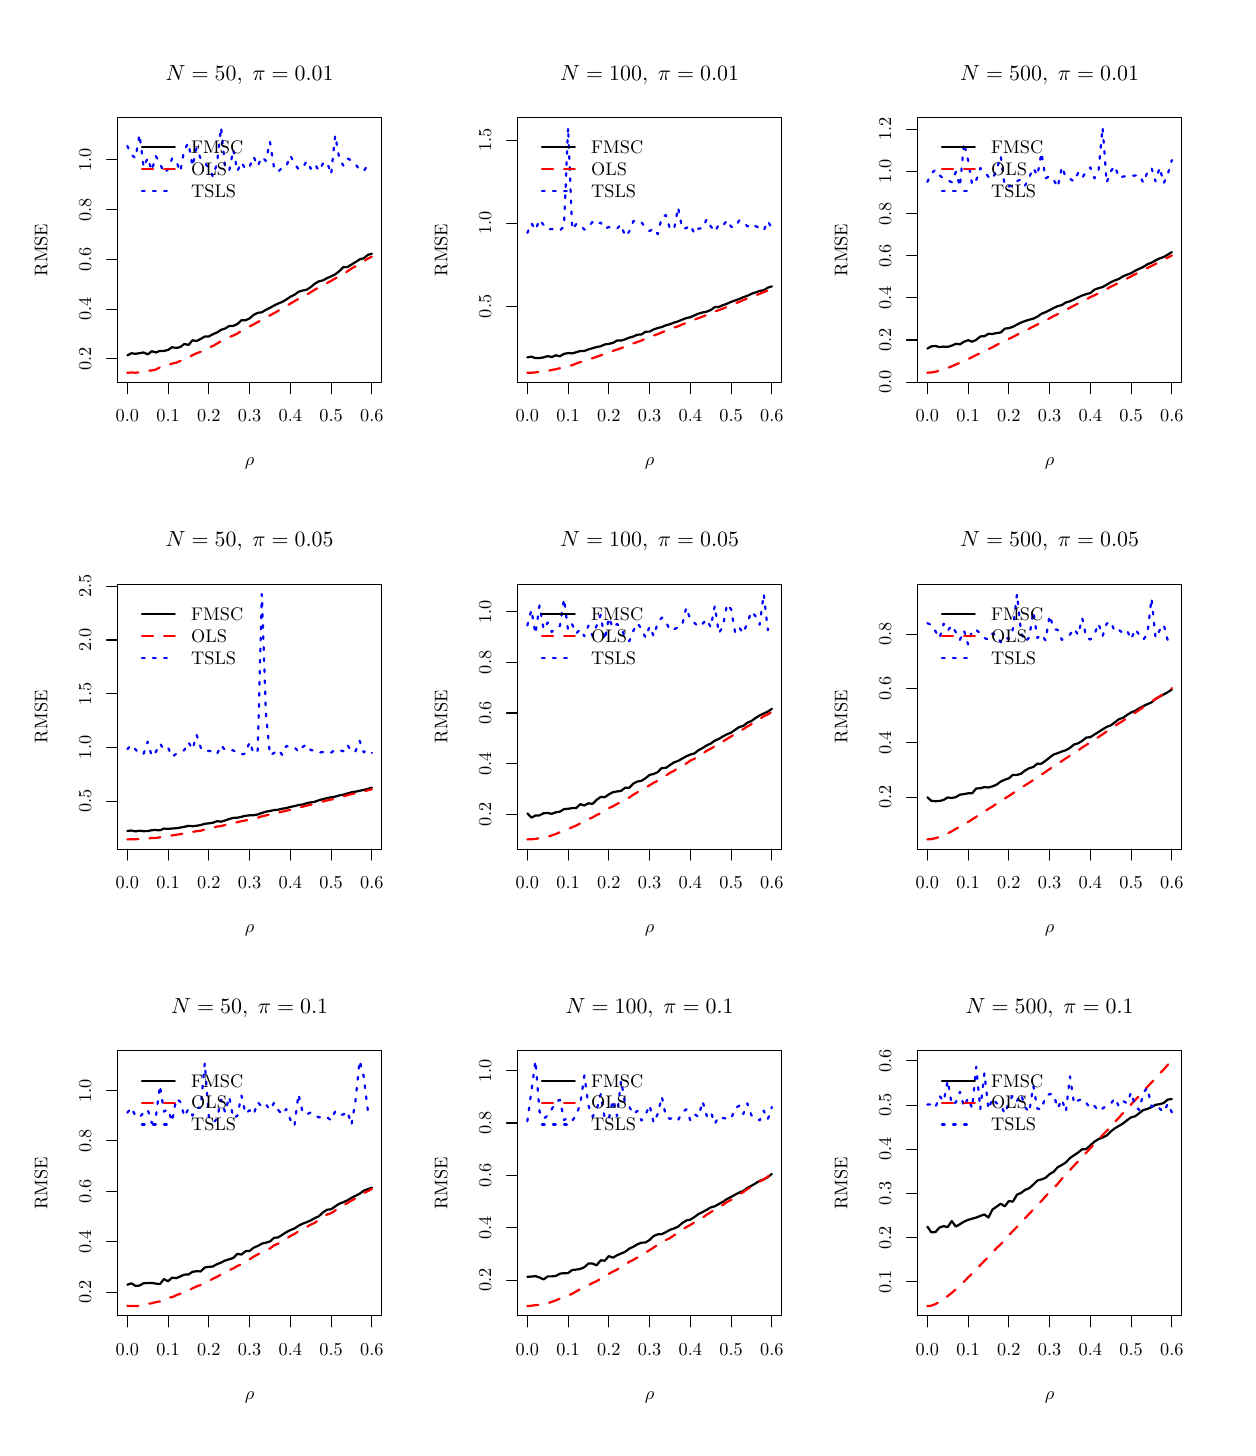
\begin{tikzpicture}[x=1pt,y=1pt]
\definecolor{fillColor}{RGB}{255,255,255}
\path[use as bounding box,fill=fillColor,fill opacity=0.00] (0,0) rectangle (433.62,505.89);
\begin{scope}
\path[clip] ( 32.47,377.65) rectangle (127.91,473.42);
\definecolor{drawColor}{RGB}{0,0,0}

\path[draw=drawColor,line width= 0.8pt,line join=round,line cap=round] ( 36.01,387.44) --
	( 37.48,388.24) --
	( 38.95,388.03) --
	( 40.42,388.27) --
	( 41.90,388.52) --
	( 43.37,387.83) --
	( 44.84,388.97) --
	( 46.32,388.51) --
	( 47.79,389.10) --
	( 49.26,389.06) --
	( 50.73,389.45) --
	( 52.21,390.43) --
	( 53.68,390.14) --
	( 55.15,390.49) --
	( 56.63,391.61) --
	( 58.10,391.24) --
	( 59.57,392.92) --
	( 61.04,392.65) --
	( 62.52,393.43) --
	( 63.99,394.26) --
	( 65.46,394.31) --
	( 66.93,395.12) --
	( 68.41,395.73) --
	( 69.88,396.69) --
	( 71.35,397.18) --
	( 72.83,398.07) --
	( 74.30,398.13) --
	( 75.77,398.78) --
	( 77.24,400.16) --
	( 78.72,400.14) --
	( 80.19,400.84) --
	( 81.66,402.11) --
	( 83.14,402.83) --
	( 84.61,403.04) --
	( 86.08,403.92) --
	( 87.55,404.64) --
	( 89.03,405.47) --
	( 90.50,406.19) --
	( 91.97,406.78) --
	( 93.44,407.64) --
	( 94.92,408.65) --
	( 96.39,409.36) --
	( 97.86,410.45) --
	( 99.34,410.90) --
	(100.81,411.18) --
	(102.28,412.12) --
	(103.75,413.39) --
	(105.23,414.22) --
	(106.70,414.58) --
	(108.17,415.37) --
	(109.65,416.03) --
	(111.12,416.74) --
	(112.59,417.90) --
	(114.06,419.32) --
	(115.54,419.40) --
	(117.01,420.28) --
	(118.48,421.19) --
	(119.95,422.16) --
	(121.43,422.55) --
	(122.90,423.77) --
	(124.37,424.21);
\end{scope}
\begin{scope}
\path[clip] (  0.00,  0.00) rectangle (433.62,505.89);
\definecolor{drawColor}{RGB}{0,0,0}

\path[draw=drawColor,line width= 0.4pt,line join=round,line cap=round] ( 36.01,377.65) -- (124.37,377.65);

\path[draw=drawColor,line width= 0.4pt,line join=round,line cap=round] ( 36.01,377.65) -- ( 36.01,373.69);

\path[draw=drawColor,line width= 0.4pt,line join=round,line cap=round] ( 50.73,377.65) -- ( 50.73,373.69);

\path[draw=drawColor,line width= 0.4pt,line join=round,line cap=round] ( 65.46,377.65) -- ( 65.46,373.69);

\path[draw=drawColor,line width= 0.4pt,line join=round,line cap=round] ( 80.19,377.65) -- ( 80.19,373.69);

\path[draw=drawColor,line width= 0.4pt,line join=round,line cap=round] ( 94.92,377.65) -- ( 94.92,373.69);

\path[draw=drawColor,line width= 0.4pt,line join=round,line cap=round] (109.65,377.65) -- (109.65,373.69);

\path[draw=drawColor,line width= 0.4pt,line join=round,line cap=round] (124.37,377.65) -- (124.37,373.69);

\node[text=drawColor,anchor=base,inner sep=0pt, outer sep=0pt, scale=  0.66] at ( 36.01,363.40) {0.0};

\node[text=drawColor,anchor=base,inner sep=0pt, outer sep=0pt, scale=  0.66] at ( 50.73,363.40) {0.1};

\node[text=drawColor,anchor=base,inner sep=0pt, outer sep=0pt, scale=  0.66] at ( 65.46,363.40) {0.2};

\node[text=drawColor,anchor=base,inner sep=0pt, outer sep=0pt, scale=  0.66] at ( 80.19,363.40) {0.3};

\node[text=drawColor,anchor=base,inner sep=0pt, outer sep=0pt, scale=  0.66] at ( 94.92,363.40) {0.4};

\node[text=drawColor,anchor=base,inner sep=0pt, outer sep=0pt, scale=  0.66] at (109.65,363.40) {0.5};

\node[text=drawColor,anchor=base,inner sep=0pt, outer sep=0pt, scale=  0.66] at (124.37,363.40) {0.6};

\path[draw=drawColor,line width= 0.4pt,line join=round,line cap=round] ( 32.47,386.18) -- ( 32.47,458.10);

\path[draw=drawColor,line width= 0.4pt,line join=round,line cap=round] ( 32.47,386.18) -- ( 28.51,386.18);

\path[draw=drawColor,line width= 0.4pt,line join=round,line cap=round] ( 32.47,404.16) -- ( 28.51,404.16);

\path[draw=drawColor,line width= 0.4pt,line join=round,line cap=round] ( 32.47,422.14) -- ( 28.51,422.14);

\path[draw=drawColor,line width= 0.4pt,line join=round,line cap=round] ( 32.47,440.12) -- ( 28.51,440.12);

\path[draw=drawColor,line width= 0.4pt,line join=round,line cap=round] ( 32.47,458.10) -- ( 28.51,458.10);

\node[text=drawColor,rotate= 90.00,anchor=base,inner sep=0pt, outer sep=0pt, scale=  0.66] at ( 22.97,386.18) {0.2};

\node[text=drawColor,rotate= 90.00,anchor=base,inner sep=0pt, outer sep=0pt, scale=  0.66] at ( 22.97,404.16) {0.4};

\node[text=drawColor,rotate= 90.00,anchor=base,inner sep=0pt, outer sep=0pt, scale=  0.66] at ( 22.97,422.14) {0.6};

\node[text=drawColor,rotate= 90.00,anchor=base,inner sep=0pt, outer sep=0pt, scale=  0.66] at ( 22.97,440.12) {0.8};

\node[text=drawColor,rotate= 90.00,anchor=base,inner sep=0pt, outer sep=0pt, scale=  0.66] at ( 22.97,458.10) {1.0};

\path[draw=drawColor,line width= 0.4pt,line join=round,line cap=round] ( 32.47,377.65) --
	(127.91,377.65) --
	(127.91,473.42) --
	( 32.47,473.42) --
	( 32.47,377.65);
\end{scope}
\begin{scope}
\path[clip] (  0.00,337.26) rectangle (144.54,505.89);
\definecolor{drawColor}{RGB}{0,0,0}

\node[text=drawColor,anchor=base,inner sep=0pt, outer sep=0pt, scale=  0.79] at ( 80.19,486.92) {\bfseries $N=50, \;\pi=0.01$};

\node[text=drawColor,anchor=base,inner sep=0pt, outer sep=0pt, scale=  0.66] at ( 80.19,347.56) {$\rho$};

\node[text=drawColor,rotate= 90.00,anchor=base,inner sep=0pt, outer sep=0pt, scale=  0.66] at (  7.13,425.53) {RMSE};
\end{scope}
\begin{scope}
\path[clip] ( 32.47,377.65) rectangle (127.91,473.42);
\definecolor{drawColor}{RGB}{255,0,0}

\path[draw=drawColor,line width= 0.8pt,dash pattern=on 4pt off 4pt ,line join=round,line cap=round] ( 36.01,381.20) --
	( 37.48,381.26) --
	( 38.95,381.21) --
	( 40.42,381.32) --
	( 41.90,381.63) --
	( 43.37,381.87) --
	( 44.84,382.04) --
	( 46.32,382.34) --
	( 47.79,383.16) --
	( 49.26,383.31) --
	( 50.73,384.03) --
	( 52.21,384.52) --
	( 53.68,384.82) --
	( 55.15,385.45) --
	( 56.63,386.11) --
	( 58.10,386.69) --
	( 59.57,387.56) --
	( 61.04,388.22) --
	( 62.52,388.76) --
	( 63.99,389.47) --
	( 65.46,390.31) --
	( 66.93,390.84) --
	( 68.41,391.73) --
	( 69.88,392.61) --
	( 71.35,393.24) --
	( 72.83,394.06) --
	( 74.30,394.64) --
	( 75.77,395.34) --
	( 77.24,396.39) --
	( 78.72,397.12) --
	( 80.19,397.96) --
	( 81.66,398.69) --
	( 83.14,399.51) --
	( 84.61,400.24) --
	( 86.08,401.22) --
	( 87.55,401.94) --
	( 89.03,402.72) --
	( 90.50,403.56) --
	( 91.97,404.43) --
	( 93.44,405.25) --
	( 94.92,406.17) --
	( 96.39,407.05) --
	( 97.86,407.89) --
	( 99.34,408.68) --
	(100.81,409.29) --
	(102.28,410.31) --
	(103.75,411.20) --
	(105.23,412.03) --
	(106.70,412.76) --
	(108.17,413.61) --
	(109.65,414.41) --
	(111.12,415.27) --
	(112.59,416.19) --
	(114.06,417.14) --
	(115.54,417.81) --
	(117.01,418.84) --
	(118.48,419.67) --
	(119.95,420.64) --
	(121.43,421.46) --
	(122.90,422.42) --
	(124.37,423.17);
\definecolor{drawColor}{RGB}{0,0,255}

\path[draw=drawColor,line width= 0.8pt,dash pattern=on 1pt off 3pt ,line join=round,line cap=round] ( 36.01,463.18) --
	( 37.48,459.93) --
	( 38.95,458.78) --
	( 40.42,467.28) --
	( 41.90,455.45) --
	( 43.37,458.84) --
	( 44.84,454.20) --
	( 46.32,459.47) --
	( 47.79,456.96) --
	( 49.26,453.36) --
	( 50.73,454.72) --
	( 52.21,458.67) --
	( 53.68,457.68) --
	( 55.15,453.88) --
	( 56.63,461.89) --
	( 58.10,464.21) --
	( 59.57,455.80) --
	( 61.04,462.43) --
	( 62.52,458.46) --
	( 63.99,457.11) --
	( 65.46,455.09) --
	( 66.93,452.12) --
	( 68.41,456.85) --
	( 69.88,469.87) --
	( 71.35,455.18) --
	( 72.83,454.19) --
	( 74.30,461.84) --
	( 75.77,454.03) --
	( 77.24,457.24) --
	( 78.72,454.73) --
	( 80.19,455.67) --
	( 81.66,459.26) --
	( 83.14,455.89) --
	( 84.61,459.17) --
	( 86.08,457.75) --
	( 87.55,464.66) --
	( 89.03,455.29) --
	( 90.50,453.79) --
	( 91.97,455.34) --
	( 93.44,455.71) --
	( 94.92,459.70) --
	( 96.39,456.77) --
	( 97.86,454.78) --
	( 99.34,455.15) --
	(100.81,457.66) --
	(102.28,454.92) --
	(103.75,456.66) --
	(105.23,454.13) --
	(106.70,456.80) --
	(108.17,457.38) --
	(109.65,452.89) --
	(111.12,466.97) --
	(112.59,458.64) --
	(114.06,456.06) --
	(115.54,458.66) --
	(117.01,457.85) --
	(118.48,456.54) --
	(119.95,454.48) --
	(121.43,454.06) --
	(122.90,456.26) --
	(124.37,456.56);
\definecolor{drawColor}{RGB}{0,0,0}

\path[draw=drawColor,line width= 0.8pt,line join=round,line cap=round] ( 41.28,462.63) -- ( 53.16,462.63);
\definecolor{drawColor}{RGB}{255,0,0}

\path[draw=drawColor,line width= 0.8pt,dash pattern=on 4pt off 4pt ,line join=round,line cap=round] ( 41.28,454.71) -- ( 53.16,454.71);
\definecolor{drawColor}{RGB}{0,0,255}

\path[draw=drawColor,line width= 0.8pt,dash pattern=on 1pt off 3pt ,line join=round,line cap=round] ( 41.28,446.79) -- ( 53.16,446.79);
\definecolor{drawColor}{RGB}{0,0,0}

\node[text=drawColor,anchor=base west,inner sep=0pt, outer sep=0pt, scale=  0.66] at ( 59.10,460.35) {FMSC};

\node[text=drawColor,anchor=base west,inner sep=0pt, outer sep=0pt, scale=  0.66] at ( 59.10,452.43) {OLS};

\node[text=drawColor,anchor=base west,inner sep=0pt, outer sep=0pt, scale=  0.66] at ( 59.10,444.51) {TSLS};
\end{scope}
\begin{scope}
\path[clip] (177.01,377.65) rectangle (272.45,473.42);
\definecolor{drawColor}{RGB}{0,0,0}

\path[draw=drawColor,line width= 0.8pt,line join=round,line cap=round] (180.55,386.74) --
	(182.02,386.99) --
	(183.49,386.49) --
	(184.96,386.50) --
	(186.44,386.74) --
	(187.91,387.21) --
	(189.38,386.87) --
	(190.86,387.50) --
	(192.33,387.15) --
	(193.80,388.03) --
	(195.27,388.31) --
	(196.75,388.18) --
	(198.22,388.60) --
	(199.69,389.07) --
	(201.17,389.08) --
	(202.64,389.63) --
	(204.11,390.06) --
	(205.58,390.48) --
	(207.06,390.76) --
	(208.53,391.42) --
	(210.00,391.63) --
	(211.47,391.96) --
	(212.95,392.83) --
	(214.42,392.82) --
	(215.89,393.26) --
	(217.37,393.88) --
	(218.84,394.29) --
	(220.31,394.94) --
	(221.78,395.02) --
	(223.26,396.03) --
	(224.73,396.06) --
	(226.20,396.85) --
	(227.68,397.36) --
	(229.15,397.71) --
	(230.62,398.34) --
	(232.09,398.74) --
	(233.57,399.31) --
	(235.04,399.76) --
	(236.51,400.38) --
	(237.98,400.93) --
	(239.46,401.27) --
	(240.93,401.92) --
	(242.40,402.56) --
	(243.88,402.97) --
	(245.35,403.26) --
	(246.82,403.87) --
	(248.29,404.92) --
	(249.77,404.99) --
	(251.24,405.62) --
	(252.71,406.13) --
	(254.19,406.81) --
	(255.66,407.33) --
	(257.13,407.84) --
	(258.60,408.50) --
	(260.08,409.01) --
	(261.55,409.72) --
	(263.02,410.21) --
	(264.50,410.77) --
	(265.97,411.01) --
	(267.44,411.93) --
	(268.91,412.41);
\end{scope}
\begin{scope}
\path[clip] (  0.00,  0.00) rectangle (433.62,505.89);
\definecolor{drawColor}{RGB}{0,0,0}

\path[draw=drawColor,line width= 0.4pt,line join=round,line cap=round] (180.55,377.65) -- (268.91,377.65);

\path[draw=drawColor,line width= 0.4pt,line join=round,line cap=round] (180.55,377.65) -- (180.55,373.69);

\path[draw=drawColor,line width= 0.4pt,line join=round,line cap=round] (195.27,377.65) -- (195.27,373.69);

\path[draw=drawColor,line width= 0.4pt,line join=round,line cap=round] (210.00,377.65) -- (210.00,373.69);

\path[draw=drawColor,line width= 0.4pt,line join=round,line cap=round] (224.73,377.65) -- (224.73,373.69);

\path[draw=drawColor,line width= 0.4pt,line join=round,line cap=round] (239.46,377.65) -- (239.46,373.69);

\path[draw=drawColor,line width= 0.4pt,line join=round,line cap=round] (254.19,377.65) -- (254.19,373.69);

\path[draw=drawColor,line width= 0.4pt,line join=round,line cap=round] (268.91,377.65) -- (268.91,373.69);

\node[text=drawColor,anchor=base,inner sep=0pt, outer sep=0pt, scale=  0.66] at (180.55,363.40) {0.0};

\node[text=drawColor,anchor=base,inner sep=0pt, outer sep=0pt, scale=  0.66] at (195.27,363.40) {0.1};

\node[text=drawColor,anchor=base,inner sep=0pt, outer sep=0pt, scale=  0.66] at (210.00,363.40) {0.2};

\node[text=drawColor,anchor=base,inner sep=0pt, outer sep=0pt, scale=  0.66] at (224.73,363.40) {0.3};

\node[text=drawColor,anchor=base,inner sep=0pt, outer sep=0pt, scale=  0.66] at (239.46,363.40) {0.4};

\node[text=drawColor,anchor=base,inner sep=0pt, outer sep=0pt, scale=  0.66] at (254.19,363.40) {0.5};

\node[text=drawColor,anchor=base,inner sep=0pt, outer sep=0pt, scale=  0.66] at (268.91,363.40) {0.6};

\path[draw=drawColor,line width= 0.4pt,line join=round,line cap=round] (177.01,405.16) -- (177.01,465.26);

\path[draw=drawColor,line width= 0.4pt,line join=round,line cap=round] (177.01,405.16) -- (173.05,405.16);

\path[draw=drawColor,line width= 0.4pt,line join=round,line cap=round] (177.01,435.21) -- (173.05,435.21);

\path[draw=drawColor,line width= 0.4pt,line join=round,line cap=round] (177.01,465.26) -- (173.05,465.26);

\node[text=drawColor,rotate= 90.00,anchor=base,inner sep=0pt, outer sep=0pt, scale=  0.66] at (167.51,405.16) {0.5};

\node[text=drawColor,rotate= 90.00,anchor=base,inner sep=0pt, outer sep=0pt, scale=  0.66] at (167.51,435.21) {1.0};

\node[text=drawColor,rotate= 90.00,anchor=base,inner sep=0pt, outer sep=0pt, scale=  0.66] at (167.51,465.26) {1.5};

\path[draw=drawColor,line width= 0.4pt,line join=round,line cap=round] (177.01,377.65) --
	(272.45,377.65) --
	(272.45,473.42) --
	(177.01,473.42) --
	(177.01,377.65);
\end{scope}
\begin{scope}
\path[clip] (144.54,337.26) rectangle (289.08,505.89);
\definecolor{drawColor}{RGB}{0,0,0}

\node[text=drawColor,anchor=base,inner sep=0pt, outer sep=0pt, scale=  0.79] at (224.73,486.92) {\bfseries $N=100, \;\pi=0.01$};

\node[text=drawColor,anchor=base,inner sep=0pt, outer sep=0pt, scale=  0.66] at (224.73,347.56) {$\rho$};

\node[text=drawColor,rotate= 90.00,anchor=base,inner sep=0pt, outer sep=0pt, scale=  0.66] at (151.67,425.53) {RMSE};
\end{scope}
\begin{scope}
\path[clip] (177.01,377.65) rectangle (272.45,473.42);
\definecolor{drawColor}{RGB}{255,0,0}

\path[draw=drawColor,line width= 0.8pt,dash pattern=on 4pt off 4pt ,line join=round,line cap=round] (180.55,381.20) --
	(182.02,381.20) --
	(183.49,381.31) --
	(184.96,381.48) --
	(186.44,381.60) --
	(187.91,381.79) --
	(189.38,382.21) --
	(190.86,382.47) --
	(192.33,382.82) --
	(193.80,383.19) --
	(195.27,383.57) --
	(196.75,383.94) --
	(198.22,384.53) --
	(199.69,385.04) --
	(201.17,385.51) --
	(202.64,385.92) --
	(204.11,386.44) --
	(205.58,386.96) --
	(207.06,387.45) --
	(208.53,388.03) --
	(210.00,388.58) --
	(211.47,389.07) --
	(212.95,389.58) --
	(214.42,390.07) --
	(215.89,390.60) --
	(217.37,391.28) --
	(218.84,391.79) --
	(220.31,392.32) --
	(221.78,392.83) --
	(223.26,393.52) --
	(224.73,394.13) --
	(226.20,394.62) --
	(227.68,395.16) --
	(229.15,395.78) --
	(230.62,396.38) --
	(232.09,396.85) --
	(233.57,397.51) --
	(235.04,398.00) --
	(236.51,398.65) --
	(237.98,399.19) --
	(239.46,399.84) --
	(240.93,400.38) --
	(242.40,400.93) --
	(243.88,401.50) --
	(245.35,402.05) --
	(246.82,402.61) --
	(248.29,403.30) --
	(249.77,403.84) --
	(251.24,404.39) --
	(252.71,404.97) --
	(254.19,405.65) --
	(255.66,406.27) --
	(257.13,406.77) --
	(258.60,407.45) --
	(260.08,408.00) --
	(261.55,408.64) --
	(263.02,409.12) --
	(264.50,409.74) --
	(265.97,410.32) --
	(267.44,410.92) --
	(268.91,411.54);
\definecolor{drawColor}{RGB}{0,0,255}

\path[draw=drawColor,line width= 0.8pt,dash pattern=on 1pt off 3pt ,line join=round,line cap=round] (180.55,431.72) --
	(182.02,435.22) --
	(183.49,432.80) --
	(184.96,436.51) --
	(186.44,434.56) --
	(187.91,432.99) --
	(189.38,433.12) --
	(190.86,432.97) --
	(192.33,432.64) --
	(193.80,434.03) --
	(195.27,469.87) --
	(196.75,432.97) --
	(198.22,434.90) --
	(199.69,434.76) --
	(201.17,432.87) --
	(202.64,433.82) --
	(204.11,435.70) --
	(205.58,434.63) --
	(207.06,435.47) --
	(208.53,433.22) --
	(210.00,433.83) --
	(211.47,433.47) --
	(212.95,433.27) --
	(214.42,434.75) --
	(215.89,430.47) --
	(217.37,432.18) --
	(218.84,435.90) --
	(220.31,436.38) --
	(221.78,435.56) --
	(223.26,433.69) --
	(224.73,432.38) --
	(226.20,433.36) --
	(227.68,431.26) --
	(229.15,437.49) --
	(230.62,438.14) --
	(232.09,433.21) --
	(233.57,433.05) --
	(235.04,440.93) --
	(236.51,433.27) --
	(237.98,433.44) --
	(239.46,434.60) --
	(240.93,431.44) --
	(242.40,433.30) --
	(243.88,433.42) --
	(245.35,436.70) --
	(246.82,434.10) --
	(248.29,432.15) --
	(249.77,434.75) --
	(251.24,434.24) --
	(252.71,436.32) --
	(254.19,433.95) --
	(255.66,433.76) --
	(257.13,436.25) --
	(258.60,435.55) --
	(260.08,434.07) --
	(261.55,434.99) --
	(263.02,434.15) --
	(264.50,433.59) --
	(265.97,432.58) --
	(267.44,435.97) --
	(268.91,433.42);
\definecolor{drawColor}{RGB}{0,0,0}

\path[draw=drawColor,line width= 0.8pt,line join=round,line cap=round] (185.82,462.63) -- (197.70,462.63);
\definecolor{drawColor}{RGB}{255,0,0}

\path[draw=drawColor,line width= 0.8pt,dash pattern=on 4pt off 4pt ,line join=round,line cap=round] (185.82,454.71) -- (197.70,454.71);
\definecolor{drawColor}{RGB}{0,0,255}

\path[draw=drawColor,line width= 0.8pt,dash pattern=on 1pt off 3pt ,line join=round,line cap=round] (185.82,446.79) -- (197.70,446.79);
\definecolor{drawColor}{RGB}{0,0,0}

\node[text=drawColor,anchor=base west,inner sep=0pt, outer sep=0pt, scale=  0.66] at (203.64,460.35) {FMSC};

\node[text=drawColor,anchor=base west,inner sep=0pt, outer sep=0pt, scale=  0.66] at (203.64,452.43) {OLS};

\node[text=drawColor,anchor=base west,inner sep=0pt, outer sep=0pt, scale=  0.66] at (203.64,444.51) {TSLS};
\end{scope}
\begin{scope}
\path[clip] (321.55,377.65) rectangle (416.99,473.42);
\definecolor{drawColor}{RGB}{0,0,0}

\path[draw=drawColor,line width= 0.8pt,line join=round,line cap=round] (325.09,389.91) --
	(326.56,390.74) --
	(328.03,390.86) --
	(329.50,390.46) --
	(330.98,390.64) --
	(332.45,390.55) --
	(333.92,390.98) --
	(335.40,391.67) --
	(336.87,391.46) --
	(338.34,392.40) --
	(339.81,392.96) --
	(341.29,392.41) --
	(342.76,393.10) --
	(344.23,394.31) --
	(345.71,394.40) --
	(347.18,395.26) --
	(348.65,395.21) --
	(350.12,395.54) --
	(351.60,395.74) --
	(353.07,397.13) --
	(354.54,397.30) --
	(356.01,397.81) --
	(357.49,398.59) --
	(358.96,399.32) --
	(360.43,399.90) --
	(361.91,400.36) --
	(363.38,400.73) --
	(364.85,401.46) --
	(366.32,402.50) --
	(367.80,403.08) --
	(369.27,403.82) --
	(370.74,404.59) --
	(372.22,405.28) --
	(373.69,405.65) --
	(375.16,406.61) --
	(376.63,407.01) --
	(378.11,407.68) --
	(379.58,408.45) --
	(381.05,409.10) --
	(382.52,409.60) --
	(384.00,409.99) --
	(385.47,411.21) --
	(386.94,411.75) --
	(388.42,412.17) --
	(389.89,413.00) --
	(391.36,413.89) --
	(392.83,414.54) --
	(394.31,415.10) --
	(395.78,416.01) --
	(397.25,416.64) --
	(398.73,417.18) --
	(400.20,418.08) --
	(401.67,418.75) --
	(403.14,419.44) --
	(404.62,420.40) --
	(406.09,420.97) --
	(407.56,421.78) --
	(409.04,422.51) --
	(410.51,423.02) --
	(411.98,423.89) --
	(413.45,424.79);
\end{scope}
\begin{scope}
\path[clip] (  0.00,  0.00) rectangle (433.62,505.89);
\definecolor{drawColor}{RGB}{0,0,0}

\path[draw=drawColor,line width= 0.4pt,line join=round,line cap=round] (325.09,377.65) -- (413.45,377.65);

\path[draw=drawColor,line width= 0.4pt,line join=round,line cap=round] (325.09,377.65) -- (325.09,373.69);

\path[draw=drawColor,line width= 0.4pt,line join=round,line cap=round] (339.81,377.65) -- (339.81,373.69);

\path[draw=drawColor,line width= 0.4pt,line join=round,line cap=round] (354.54,377.65) -- (354.54,373.69);

\path[draw=drawColor,line width= 0.4pt,line join=round,line cap=round] (369.27,377.65) -- (369.27,373.69);

\path[draw=drawColor,line width= 0.4pt,line join=round,line cap=round] (384.00,377.65) -- (384.00,373.69);

\path[draw=drawColor,line width= 0.4pt,line join=round,line cap=round] (398.73,377.65) -- (398.73,373.69);

\path[draw=drawColor,line width= 0.4pt,line join=round,line cap=round] (413.45,377.65) -- (413.45,373.69);

\node[text=drawColor,anchor=base,inner sep=0pt, outer sep=0pt, scale=  0.66] at (325.09,363.40) {0.0};

\node[text=drawColor,anchor=base,inner sep=0pt, outer sep=0pt, scale=  0.66] at (339.81,363.40) {0.1};

\node[text=drawColor,anchor=base,inner sep=0pt, outer sep=0pt, scale=  0.66] at (354.54,363.40) {0.2};

\node[text=drawColor,anchor=base,inner sep=0pt, outer sep=0pt, scale=  0.66] at (369.27,363.40) {0.3};

\node[text=drawColor,anchor=base,inner sep=0pt, outer sep=0pt, scale=  0.66] at (384.00,363.40) {0.4};

\node[text=drawColor,anchor=base,inner sep=0pt, outer sep=0pt, scale=  0.66] at (398.73,363.40) {0.5};

\node[text=drawColor,anchor=base,inner sep=0pt, outer sep=0pt, scale=  0.66] at (413.45,363.40) {0.6};

\path[draw=drawColor,line width= 0.4pt,line join=round,line cap=round] (321.55,377.82) -- (321.55,469.18);

\path[draw=drawColor,line width= 0.4pt,line join=round,line cap=round] (321.55,377.82) -- (317.59,377.82);

\path[draw=drawColor,line width= 0.4pt,line join=round,line cap=round] (321.55,393.04) -- (317.59,393.04);

\path[draw=drawColor,line width= 0.4pt,line join=round,line cap=round] (321.55,408.27) -- (317.59,408.27);

\path[draw=drawColor,line width= 0.4pt,line join=round,line cap=round] (321.55,423.50) -- (317.59,423.50);

\path[draw=drawColor,line width= 0.4pt,line join=round,line cap=round] (321.55,438.72) -- (317.59,438.72);

\path[draw=drawColor,line width= 0.4pt,line join=round,line cap=round] (321.55,453.95) -- (317.59,453.95);

\path[draw=drawColor,line width= 0.4pt,line join=round,line cap=round] (321.55,469.18) -- (317.59,469.18);

\node[text=drawColor,rotate= 90.00,anchor=base,inner sep=0pt, outer sep=0pt, scale=  0.66] at (312.05,377.82) {0.0};

\node[text=drawColor,rotate= 90.00,anchor=base,inner sep=0pt, outer sep=0pt, scale=  0.66] at (312.05,393.04) {0.2};

\node[text=drawColor,rotate= 90.00,anchor=base,inner sep=0pt, outer sep=0pt, scale=  0.66] at (312.05,408.27) {0.4};

\node[text=drawColor,rotate= 90.00,anchor=base,inner sep=0pt, outer sep=0pt, scale=  0.66] at (312.05,423.50) {0.6};

\node[text=drawColor,rotate= 90.00,anchor=base,inner sep=0pt, outer sep=0pt, scale=  0.66] at (312.05,438.72) {0.8};

\node[text=drawColor,rotate= 90.00,anchor=base,inner sep=0pt, outer sep=0pt, scale=  0.66] at (312.05,453.95) {1.0};

\node[text=drawColor,rotate= 90.00,anchor=base,inner sep=0pt, outer sep=0pt, scale=  0.66] at (312.05,469.18) {1.2};

\path[draw=drawColor,line width= 0.4pt,line join=round,line cap=round] (321.55,377.65) --
	(416.99,377.65) --
	(416.99,473.42) --
	(321.55,473.42) --
	(321.55,377.65);
\end{scope}
\begin{scope}
\path[clip] (289.08,337.26) rectangle (433.62,505.89);
\definecolor{drawColor}{RGB}{0,0,0}

\node[text=drawColor,anchor=base,inner sep=0pt, outer sep=0pt, scale=  0.79] at (369.27,486.92) {\bfseries $N=500, \;\pi=0.01$};

\node[text=drawColor,anchor=base,inner sep=0pt, outer sep=0pt, scale=  0.66] at (369.27,347.56) {$\rho$};

\node[text=drawColor,rotate= 90.00,anchor=base,inner sep=0pt, outer sep=0pt, scale=  0.66] at (296.21,425.53) {RMSE};
\end{scope}
\begin{scope}
\path[clip] (321.55,377.65) rectangle (416.99,473.42);
\definecolor{drawColor}{RGB}{255,0,0}

\path[draw=drawColor,line width= 0.8pt,dash pattern=on 4pt off 4pt ,line join=round,line cap=round] (325.09,381.20) --
	(326.56,381.31) --
	(328.03,381.55) --
	(329.50,381.96) --
	(330.98,382.39) --
	(332.45,382.91) --
	(333.92,383.52) --
	(335.40,384.16) --
	(336.87,384.81) --
	(338.34,385.44) --
	(339.81,386.09) --
	(341.29,386.86) --
	(342.76,387.61) --
	(344.23,388.28) --
	(345.71,389.01) --
	(347.18,389.72) --
	(348.65,390.45) --
	(350.12,391.21) --
	(351.60,391.92) --
	(353.07,392.65) --
	(354.54,393.42) --
	(356.01,394.12) --
	(357.49,394.90) --
	(358.96,395.64) --
	(360.43,396.45) --
	(361.91,397.12) --
	(363.38,397.89) --
	(364.85,398.62) --
	(366.32,399.43) --
	(367.80,400.15) --
	(369.27,400.86) --
	(370.74,401.68) --
	(372.22,402.40) --
	(373.69,403.16) --
	(375.16,403.90) --
	(376.63,404.70) --
	(378.11,405.47) --
	(379.58,406.20) --
	(381.05,406.91) --
	(382.52,407.71) --
	(384.00,408.53) --
	(385.47,409.17) --
	(386.94,409.93) --
	(388.42,410.69) --
	(389.89,411.46) --
	(391.36,412.28) --
	(392.83,412.97) --
	(394.31,413.70) --
	(395.78,414.47) --
	(397.25,415.25) --
	(398.73,416.04) --
	(400.20,416.81) --
	(401.67,417.54) --
	(403.14,418.29) --
	(404.62,419.03) --
	(406.09,419.81) --
	(407.56,420.51) --
	(409.04,421.30) --
	(410.51,422.08) --
	(411.98,422.83) --
	(413.45,423.54);
\definecolor{drawColor}{RGB}{0,0,255}

\path[draw=drawColor,line width= 0.8pt,dash pattern=on 1pt off 3pt ,line join=round,line cap=round] (325.09,450.14) --
	(326.56,453.21) --
	(328.03,454.54) --
	(329.50,452.50) --
	(330.98,451.40) --
	(332.45,450.66) --
	(333.92,450.08) --
	(335.40,453.79) --
	(336.87,448.50) --
	(338.34,464.24) --
	(339.81,458.00) --
	(341.29,449.08) --
	(342.76,450.76) --
	(344.23,455.14) --
	(345.71,453.99) --
	(347.18,451.99) --
	(348.65,451.11) --
	(350.12,454.52) --
	(351.60,459.51) --
	(353.07,448.48) --
	(354.54,448.55) --
	(356.01,448.74) --
	(357.49,450.42) --
	(358.96,451.07) --
	(360.43,448.86) --
	(361.91,451.86) --
	(363.38,455.18) --
	(364.85,452.46) --
	(366.32,460.68) --
	(367.80,451.45) --
	(369.27,452.24) --
	(370.74,450.88) --
	(372.22,448.23) --
	(373.69,455.60) --
	(375.16,451.73) --
	(376.63,451.29) --
	(378.11,450.31) --
	(379.58,453.40) --
	(381.05,451.51) --
	(382.52,454.08) --
	(384.00,455.38) --
	(385.47,451.44) --
	(386.94,454.11) --
	(388.42,469.87) --
	(389.89,449.84) --
	(391.36,453.97) --
	(392.83,455.93) --
	(394.31,451.70) --
	(395.78,452.07) --
	(397.25,452.27) --
	(398.73,452.31) --
	(400.20,452.47) --
	(401.67,452.67) --
	(403.14,449.85) --
	(404.62,453.74) --
	(406.09,455.24) --
	(407.56,450.36) --
	(409.04,455.33) --
	(410.51,449.68) --
	(411.98,452.96) --
	(413.45,458.07);
\definecolor{drawColor}{RGB}{0,0,0}

\path[draw=drawColor,line width= 0.8pt,line join=round,line cap=round] (330.36,462.63) -- (342.24,462.63);
\definecolor{drawColor}{RGB}{255,0,0}

\path[draw=drawColor,line width= 0.8pt,dash pattern=on 4pt off 4pt ,line join=round,line cap=round] (330.36,454.71) -- (342.24,454.71);
\definecolor{drawColor}{RGB}{0,0,255}

\path[draw=drawColor,line width= 0.8pt,dash pattern=on 1pt off 3pt ,line join=round,line cap=round] (330.36,446.79) -- (342.24,446.79);
\definecolor{drawColor}{RGB}{0,0,0}

\node[text=drawColor,anchor=base west,inner sep=0pt, outer sep=0pt, scale=  0.66] at (348.18,460.35) {FMSC};

\node[text=drawColor,anchor=base west,inner sep=0pt, outer sep=0pt, scale=  0.66] at (348.18,452.43) {OLS};

\node[text=drawColor,anchor=base west,inner sep=0pt, outer sep=0pt, scale=  0.66] at (348.18,444.51) {TSLS};
\end{scope}
\begin{scope}
\path[clip] ( 32.47,209.02) rectangle (127.91,304.79);
\definecolor{drawColor}{RGB}{0,0,0}

\path[draw=drawColor,line width= 0.8pt,line join=round,line cap=round] ( 36.01,215.62) --
	( 37.48,215.77) --
	( 38.95,215.47) --
	( 40.42,215.71) --
	( 41.90,215.55) --
	( 43.37,215.56) --
	( 44.84,215.90) --
	( 46.32,215.96) --
	( 47.79,215.83) --
	( 49.26,216.49) --
	( 50.73,216.36) --
	( 52.21,216.51) --
	( 53.68,216.60) --
	( 55.15,216.85) --
	( 56.63,217.12) --
	( 58.10,217.47) --
	( 59.57,217.33) --
	( 61.04,217.50) --
	( 62.52,217.75) --
	( 63.99,218.22) --
	( 65.46,218.36) --
	( 66.93,218.58) --
	( 68.41,219.16) --
	( 69.88,218.97) --
	( 71.35,219.42) --
	( 72.83,219.94) --
	( 74.30,220.34) --
	( 75.77,220.42) --
	( 77.24,220.72) --
	( 78.72,221.09) --
	( 80.19,221.26) --
	( 81.66,221.31) --
	( 83.14,221.59) --
	( 84.61,222.10) --
	( 86.08,222.58) --
	( 87.55,222.85) --
	( 89.03,223.16) --
	( 90.50,223.28) --
	( 91.97,223.67) --
	( 93.44,223.88) --
	( 94.92,224.29) --
	( 96.39,224.60) --
	( 97.86,224.99) --
	( 99.34,225.17) --
	(100.81,225.67) --
	(102.28,225.94) --
	(103.75,226.17) --
	(105.23,226.71) --
	(106.70,227.12) --
	(108.17,227.49) --
	(109.65,227.79) --
	(111.12,228.02) --
	(112.59,228.46) --
	(114.06,228.72) --
	(115.54,229.16) --
	(117.01,229.59) --
	(118.48,229.83) --
	(119.95,230.13) --
	(121.43,230.46) --
	(122.90,230.79) --
	(124.37,231.28);
\end{scope}
\begin{scope}
\path[clip] (  0.00,  0.00) rectangle (433.62,505.89);
\definecolor{drawColor}{RGB}{0,0,0}

\path[draw=drawColor,line width= 0.4pt,line join=round,line cap=round] ( 36.01,209.02) -- (124.37,209.02);

\path[draw=drawColor,line width= 0.4pt,line join=round,line cap=round] ( 36.01,209.02) -- ( 36.01,205.06);

\path[draw=drawColor,line width= 0.4pt,line join=round,line cap=round] ( 50.73,209.02) -- ( 50.73,205.06);

\path[draw=drawColor,line width= 0.4pt,line join=round,line cap=round] ( 65.46,209.02) -- ( 65.46,205.06);

\path[draw=drawColor,line width= 0.4pt,line join=round,line cap=round] ( 80.19,209.02) -- ( 80.19,205.06);

\path[draw=drawColor,line width= 0.4pt,line join=round,line cap=round] ( 94.92,209.02) -- ( 94.92,205.06);

\path[draw=drawColor,line width= 0.4pt,line join=round,line cap=round] (109.65,209.02) -- (109.65,205.06);

\path[draw=drawColor,line width= 0.4pt,line join=round,line cap=round] (124.37,209.02) -- (124.37,205.06);

\node[text=drawColor,anchor=base,inner sep=0pt, outer sep=0pt, scale=  0.66] at ( 36.01,194.77) {0.0};

\node[text=drawColor,anchor=base,inner sep=0pt, outer sep=0pt, scale=  0.66] at ( 50.73,194.77) {0.1};

\node[text=drawColor,anchor=base,inner sep=0pt, outer sep=0pt, scale=  0.66] at ( 65.46,194.77) {0.2};

\node[text=drawColor,anchor=base,inner sep=0pt, outer sep=0pt, scale=  0.66] at ( 80.19,194.77) {0.3};

\node[text=drawColor,anchor=base,inner sep=0pt, outer sep=0pt, scale=  0.66] at ( 94.92,194.77) {0.4};

\node[text=drawColor,anchor=base,inner sep=0pt, outer sep=0pt, scale=  0.66] at (109.65,194.77) {0.5};

\node[text=drawColor,anchor=base,inner sep=0pt, outer sep=0pt, scale=  0.66] at (124.37,194.77) {0.6};

\path[draw=drawColor,line width= 0.4pt,line join=round,line cap=round] ( 32.47,226.38) -- ( 32.47,304.04);

\path[draw=drawColor,line width= 0.4pt,line join=round,line cap=round] ( 32.47,226.38) -- ( 28.51,226.38);

\path[draw=drawColor,line width= 0.4pt,line join=round,line cap=round] ( 32.47,245.80) -- ( 28.51,245.80);

\path[draw=drawColor,line width= 0.4pt,line join=round,line cap=round] ( 32.47,265.21) -- ( 28.51,265.21);

\path[draw=drawColor,line width= 0.4pt,line join=round,line cap=round] ( 32.47,284.63) -- ( 28.51,284.63);

\path[draw=drawColor,line width= 0.4pt,line join=round,line cap=round] ( 32.47,304.04) -- ( 28.51,304.04);

\node[text=drawColor,rotate= 90.00,anchor=base,inner sep=0pt, outer sep=0pt, scale=  0.66] at ( 22.97,226.38) {0.5};

\node[text=drawColor,rotate= 90.00,anchor=base,inner sep=0pt, outer sep=0pt, scale=  0.66] at ( 22.97,245.80) {1.0};

\node[text=drawColor,rotate= 90.00,anchor=base,inner sep=0pt, outer sep=0pt, scale=  0.66] at ( 22.97,265.21) {1.5};

\node[text=drawColor,rotate= 90.00,anchor=base,inner sep=0pt, outer sep=0pt, scale=  0.66] at ( 22.97,284.63) {2.0};

\node[text=drawColor,rotate= 90.00,anchor=base,inner sep=0pt, outer sep=0pt, scale=  0.66] at ( 22.97,304.04) {2.5};

\path[draw=drawColor,line width= 0.4pt,line join=round,line cap=round] ( 32.47,209.02) --
	(127.91,209.02) --
	(127.91,304.79) --
	( 32.47,304.79) --
	( 32.47,209.02);
\end{scope}
\begin{scope}
\path[clip] (  0.00,168.63) rectangle (144.54,337.26);
\definecolor{drawColor}{RGB}{0,0,0}

\node[text=drawColor,anchor=base,inner sep=0pt, outer sep=0pt, scale=  0.79] at ( 80.19,318.29) {\bfseries $N=50, \;\pi=0.05$};

\node[text=drawColor,anchor=base,inner sep=0pt, outer sep=0pt, scale=  0.66] at ( 80.19,178.93) {$\rho$};

\node[text=drawColor,rotate= 90.00,anchor=base,inner sep=0pt, outer sep=0pt, scale=  0.66] at (  7.13,256.90) {RMSE};
\end{scope}
\begin{scope}
\path[clip] ( 32.47,209.02) rectangle (127.91,304.79);
\definecolor{drawColor}{RGB}{255,0,0}

\path[draw=drawColor,line width= 0.8pt,dash pattern=on 4pt off 4pt ,line join=round,line cap=round] ( 36.01,212.57) --
	( 37.48,212.60) --
	( 38.95,212.65) --
	( 40.42,212.69) --
	( 41.90,212.81) --
	( 43.37,212.93) --
	( 44.84,213.05) --
	( 46.32,213.10) --
	( 47.79,213.33) --
	( 49.26,213.53) --
	( 50.73,213.76) --
	( 52.21,213.99) --
	( 53.68,214.26) --
	( 55.15,214.45) --
	( 56.63,214.73) --
	( 58.10,214.94) --
	( 59.57,215.29) --
	( 61.04,215.53) --
	( 62.52,215.70) --
	( 63.99,216.17) --
	( 65.46,216.39) --
	( 66.93,216.74) --
	( 68.41,217.20) --
	( 69.88,217.37) --
	( 71.35,217.78) --
	( 72.83,218.17) --
	( 74.30,218.46) --
	( 75.77,218.78) --
	( 77.24,219.16) --
	( 78.72,219.41) --
	( 80.19,219.85) --
	( 81.66,220.12) --
	( 83.14,220.41) --
	( 84.61,220.90) --
	( 86.08,221.23) --
	( 87.55,221.57) --
	( 89.03,221.97) --
	( 90.50,222.24) --
	( 91.97,222.59) --
	( 93.44,222.94) --
	( 94.92,223.27) --
	( 96.39,223.72) --
	( 97.86,223.97) --
	( 99.34,224.39) --
	(100.81,224.78) --
	(102.28,225.09) --
	(103.75,225.52) --
	(105.23,225.89) --
	(106.70,226.27) --
	(108.17,226.65) --
	(109.65,226.96) --
	(111.12,227.28) --
	(112.59,227.71) --
	(114.06,228.07) --
	(115.54,228.53) --
	(117.01,228.94) --
	(118.48,229.22) --
	(119.95,229.55) --
	(121.43,229.93) --
	(122.90,230.32) --
	(124.37,230.68);
\definecolor{drawColor}{RGB}{0,0,255}

\path[draw=drawColor,line width= 0.8pt,dash pattern=on 1pt off 3pt ,line join=round,line cap=round] ( 36.01,245.17) --
	( 37.48,246.72) --
	( 38.95,245.11) --
	( 40.42,243.41) --
	( 41.90,243.55) --
	( 43.37,247.88) --
	( 44.84,242.63) --
	( 46.32,244.21) --
	( 47.79,247.19) --
	( 49.26,245.12) --
	( 50.73,245.73) --
	( 52.21,242.43) --
	( 53.68,243.48) --
	( 55.15,243.96) --
	( 56.63,244.87) --
	( 58.10,247.69) --
	( 59.57,245.14) --
	( 61.04,250.35) --
	( 62.52,245.76) --
	( 63.99,244.29) --
	( 65.46,244.57) --
	( 66.93,244.36) --
	( 68.41,243.37) --
	( 69.88,246.62) --
	( 71.35,244.86) --
	( 72.83,244.94) --
	( 74.30,244.74) --
	( 75.77,243.51) --
	( 77.24,243.32) --
	( 78.72,243.58) --
	( 80.19,247.83) --
	( 81.66,243.56) --
	( 83.14,244.71) --
	( 84.61,301.24) --
	( 86.08,258.22) --
	( 87.55,243.04) --
	( 89.03,243.78) --
	( 90.50,244.99) --
	( 91.97,243.14) --
	( 93.44,246.33) --
	( 94.92,245.98) --
	( 96.39,245.95) --
	( 97.86,244.19) --
	( 99.34,245.95) --
	(100.81,246.89) --
	(102.28,244.83) --
	(103.75,244.62) --
	(105.23,243.93) --
	(106.70,244.14) --
	(108.17,244.45) --
	(109.65,243.93) --
	(111.12,244.98) --
	(112.59,244.87) --
	(114.06,244.40) --
	(115.54,246.75) --
	(117.01,244.16) --
	(118.48,244.46) --
	(119.95,248.18) --
	(121.43,244.04) --
	(122.90,244.91) --
	(124.37,243.85);
\definecolor{drawColor}{RGB}{0,0,0}

\path[draw=drawColor,line width= 0.8pt,line join=round,line cap=round] ( 41.28,294.00) -- ( 53.16,294.00);
\definecolor{drawColor}{RGB}{255,0,0}

\path[draw=drawColor,line width= 0.8pt,dash pattern=on 4pt off 4pt ,line join=round,line cap=round] ( 41.28,286.08) -- ( 53.16,286.08);
\definecolor{drawColor}{RGB}{0,0,255}

\path[draw=drawColor,line width= 0.8pt,dash pattern=on 1pt off 3pt ,line join=round,line cap=round] ( 41.28,278.16) -- ( 53.16,278.16);
\definecolor{drawColor}{RGB}{0,0,0}

\node[text=drawColor,anchor=base west,inner sep=0pt, outer sep=0pt, scale=  0.66] at ( 59.10,291.72) {FMSC};

\node[text=drawColor,anchor=base west,inner sep=0pt, outer sep=0pt, scale=  0.66] at ( 59.10,283.80) {OLS};

\node[text=drawColor,anchor=base west,inner sep=0pt, outer sep=0pt, scale=  0.66] at ( 59.10,275.88) {TSLS};
\end{scope}
\begin{scope}
\path[clip] (177.01,209.02) rectangle (272.45,304.79);
\definecolor{drawColor}{RGB}{0,0,0}

\path[draw=drawColor,line width= 0.8pt,line join=round,line cap=round] (180.55,222.00) --
	(182.02,220.45) --
	(183.49,221.19) --
	(184.96,221.25) --
	(186.44,222.02) --
	(187.91,222.12) --
	(189.38,221.82) --
	(190.86,222.37) --
	(192.33,222.59) --
	(193.80,223.51) --
	(195.27,223.63) --
	(196.75,223.86) --
	(198.22,223.92) --
	(199.69,225.29) --
	(201.17,224.83) --
	(202.64,225.62) --
	(204.11,225.40) --
	(205.58,226.85) --
	(207.06,227.92) --
	(208.53,227.82) --
	(210.00,228.84) --
	(211.47,229.62) --
	(212.95,229.89) --
	(214.42,230.10) --
	(215.89,231.26) --
	(217.37,231.19) --
	(218.84,232.73) --
	(220.31,233.48) --
	(221.78,233.73) --
	(223.26,234.66) --
	(224.73,235.87) --
	(226.20,236.21) --
	(227.68,236.90) --
	(229.15,238.39) --
	(230.62,238.42) --
	(232.09,239.45) --
	(233.57,240.40) --
	(235.04,240.93) --
	(236.51,241.75) --
	(237.98,242.59) --
	(239.46,243.23) --
	(240.93,243.63) --
	(242.40,244.80) --
	(243.88,245.60) --
	(245.35,246.53) --
	(246.82,247.20) --
	(248.29,248.26) --
	(249.77,248.88) --
	(251.24,249.80) --
	(252.71,250.57) --
	(254.19,251.15) --
	(255.66,252.18) --
	(257.13,253.16) --
	(258.60,253.58) --
	(260.08,254.76) --
	(261.55,255.34) --
	(263.02,256.45) --
	(264.50,257.36) --
	(265.97,258.07) --
	(267.44,258.75) --
	(268.91,259.75);
\end{scope}
\begin{scope}
\path[clip] (  0.00,  0.00) rectangle (433.62,505.89);
\definecolor{drawColor}{RGB}{0,0,0}

\path[draw=drawColor,line width= 0.4pt,line join=round,line cap=round] (180.55,209.02) -- (268.91,209.02);

\path[draw=drawColor,line width= 0.4pt,line join=round,line cap=round] (180.55,209.02) -- (180.55,205.06);

\path[draw=drawColor,line width= 0.4pt,line join=round,line cap=round] (195.27,209.02) -- (195.27,205.06);

\path[draw=drawColor,line width= 0.4pt,line join=round,line cap=round] (210.00,209.02) -- (210.00,205.06);

\path[draw=drawColor,line width= 0.4pt,line join=round,line cap=round] (224.73,209.02) -- (224.73,205.06);

\path[draw=drawColor,line width= 0.4pt,line join=round,line cap=round] (239.46,209.02) -- (239.46,205.06);

\path[draw=drawColor,line width= 0.4pt,line join=round,line cap=round] (254.19,209.02) -- (254.19,205.06);

\path[draw=drawColor,line width= 0.4pt,line join=round,line cap=round] (268.91,209.02) -- (268.91,205.06);

\node[text=drawColor,anchor=base,inner sep=0pt, outer sep=0pt, scale=  0.66] at (180.55,194.77) {0.0};

\node[text=drawColor,anchor=base,inner sep=0pt, outer sep=0pt, scale=  0.66] at (195.27,194.77) {0.1};

\node[text=drawColor,anchor=base,inner sep=0pt, outer sep=0pt, scale=  0.66] at (210.00,194.77) {0.2};

\node[text=drawColor,anchor=base,inner sep=0pt, outer sep=0pt, scale=  0.66] at (224.73,194.77) {0.3};

\node[text=drawColor,anchor=base,inner sep=0pt, outer sep=0pt, scale=  0.66] at (239.46,194.77) {0.4};

\node[text=drawColor,anchor=base,inner sep=0pt, outer sep=0pt, scale=  0.66] at (254.19,194.77) {0.5};

\node[text=drawColor,anchor=base,inner sep=0pt, outer sep=0pt, scale=  0.66] at (268.91,194.77) {0.6};

\path[draw=drawColor,line width= 0.4pt,line join=round,line cap=round] (177.01,221.63) -- (177.01,294.84);

\path[draw=drawColor,line width= 0.4pt,line join=round,line cap=round] (177.01,221.63) -- (173.05,221.63);

\path[draw=drawColor,line width= 0.4pt,line join=round,line cap=round] (177.01,239.93) -- (173.05,239.93);

\path[draw=drawColor,line width= 0.4pt,line join=round,line cap=round] (177.01,258.24) -- (173.05,258.24);

\path[draw=drawColor,line width= 0.4pt,line join=round,line cap=round] (177.01,276.54) -- (173.05,276.54);

\path[draw=drawColor,line width= 0.4pt,line join=round,line cap=round] (177.01,294.84) -- (173.05,294.84);

\node[text=drawColor,rotate= 90.00,anchor=base,inner sep=0pt, outer sep=0pt, scale=  0.66] at (167.51,221.63) {0.2};

\node[text=drawColor,rotate= 90.00,anchor=base,inner sep=0pt, outer sep=0pt, scale=  0.66] at (167.51,239.93) {0.4};

\node[text=drawColor,rotate= 90.00,anchor=base,inner sep=0pt, outer sep=0pt, scale=  0.66] at (167.51,258.24) {0.6};

\node[text=drawColor,rotate= 90.00,anchor=base,inner sep=0pt, outer sep=0pt, scale=  0.66] at (167.51,276.54) {0.8};

\node[text=drawColor,rotate= 90.00,anchor=base,inner sep=0pt, outer sep=0pt, scale=  0.66] at (167.51,294.84) {1.0};

\path[draw=drawColor,line width= 0.4pt,line join=round,line cap=round] (177.01,209.02) --
	(272.45,209.02) --
	(272.45,304.79) --
	(177.01,304.79) --
	(177.01,209.02);
\end{scope}
\begin{scope}
\path[clip] (144.54,168.63) rectangle (289.08,337.26);
\definecolor{drawColor}{RGB}{0,0,0}

\node[text=drawColor,anchor=base,inner sep=0pt, outer sep=0pt, scale=  0.79] at (224.73,318.29) {\bfseries $N=100, \;\pi=0.05$};

\node[text=drawColor,anchor=base,inner sep=0pt, outer sep=0pt, scale=  0.66] at (224.73,178.93) {$\rho$};

\node[text=drawColor,rotate= 90.00,anchor=base,inner sep=0pt, outer sep=0pt, scale=  0.66] at (151.67,256.90) {RMSE};
\end{scope}
\begin{scope}
\path[clip] (177.01,209.02) rectangle (272.45,304.79);
\definecolor{drawColor}{RGB}{255,0,0}

\path[draw=drawColor,line width= 0.8pt,dash pattern=on 4pt off 4pt ,line join=round,line cap=round] (180.55,212.57) --
	(182.02,212.62) --
	(183.49,212.75) --
	(184.96,213.03) --
	(186.44,213.26) --
	(187.91,213.49) --
	(189.38,214.04) --
	(190.86,214.52) --
	(192.33,215.18) --
	(193.80,215.66) --
	(195.27,216.38) --
	(196.75,216.96) --
	(198.22,217.58) --
	(199.69,218.35) --
	(201.17,218.96) --
	(202.64,219.82) --
	(204.11,220.52) --
	(205.58,221.38) --
	(207.06,222.03) --
	(208.53,223.04) --
	(210.00,223.90) --
	(211.47,224.51) --
	(212.95,225.39) --
	(214.42,225.97) --
	(215.89,227.02) --
	(217.37,227.67) --
	(218.84,228.73) --
	(220.31,229.58) --
	(221.78,230.37) --
	(223.26,231.22) --
	(224.73,232.13) --
	(226.20,233.04) --
	(227.68,233.72) --
	(229.15,234.86) --
	(230.62,235.65) --
	(232.09,236.62) --
	(233.57,237.37) --
	(235.04,238.46) --
	(236.51,239.30) --
	(237.98,240.01) --
	(239.46,241.03) --
	(240.93,241.73) --
	(242.40,242.58) --
	(243.88,243.59) --
	(245.35,244.56) --
	(246.82,245.35) --
	(248.29,246.19) --
	(249.77,247.16) --
	(251.24,247.93) --
	(252.71,248.88) --
	(254.19,249.80) --
	(255.66,250.59) --
	(257.13,251.52) --
	(258.60,252.41) --
	(260.08,253.39) --
	(261.55,254.21) --
	(263.02,255.11) --
	(264.50,256.05) --
	(265.97,257.04) --
	(267.44,257.74) --
	(268.91,258.69);
\definecolor{drawColor}{RGB}{0,0,255}

\path[draw=drawColor,line width= 0.8pt,dash pattern=on 1pt off 3pt ,line join=round,line cap=round] (180.55,289.88) --
	(182.02,295.51) --
	(183.49,286.84) --
	(184.96,297.15) --
	(186.44,288.46) --
	(187.91,290.94) --
	(189.38,287.53) --
	(190.86,289.14) --
	(192.33,289.70) --
	(193.80,299.49) --
	(195.27,288.18) --
	(196.75,290.27) --
	(198.22,286.98) --
	(199.69,288.52) --
	(201.17,285.99) --
	(202.64,289.80) --
	(204.11,286.09) --
	(205.58,289.80) --
	(207.06,293.68) --
	(208.53,284.58) --
	(210.00,292.70) --
	(211.47,289.01) --
	(212.95,290.39) --
	(214.42,288.95) --
	(215.89,285.65) --
	(217.37,284.19) --
	(218.84,287.88) --
	(220.31,290.67) --
	(221.78,288.72) --
	(223.26,285.50) --
	(224.73,289.51) --
	(226.20,286.01) --
	(227.68,290.91) --
	(229.15,292.72) --
	(230.62,291.25) --
	(232.09,288.12) --
	(233.57,288.52) --
	(235.04,289.22) --
	(236.51,290.07) --
	(237.98,296.33) --
	(239.46,292.00) --
	(240.93,290.81) --
	(242.40,289.37) --
	(243.88,290.51) --
	(245.35,292.09) --
	(246.82,289.23) --
	(248.29,296.96) --
	(249.77,287.03) --
	(251.24,289.67) --
	(252.71,297.55) --
	(254.19,295.76) --
	(255.66,287.21) --
	(257.13,289.08) --
	(258.60,287.03) --
	(260.08,291.00) --
	(261.55,294.92) --
	(263.02,293.24) --
	(264.50,290.15) --
	(265.97,301.24) --
	(267.44,288.21) --
	(268.91,290.85);
\definecolor{drawColor}{RGB}{0,0,0}

\path[draw=drawColor,line width= 0.8pt,line join=round,line cap=round] (185.82,294.00) -- (197.70,294.00);
\definecolor{drawColor}{RGB}{255,0,0}

\path[draw=drawColor,line width= 0.8pt,dash pattern=on 4pt off 4pt ,line join=round,line cap=round] (185.82,286.08) -- (197.70,286.08);
\definecolor{drawColor}{RGB}{0,0,255}

\path[draw=drawColor,line width= 0.8pt,dash pattern=on 1pt off 3pt ,line join=round,line cap=round] (185.82,278.16) -- (197.70,278.16);
\definecolor{drawColor}{RGB}{0,0,0}

\node[text=drawColor,anchor=base west,inner sep=0pt, outer sep=0pt, scale=  0.66] at (203.64,291.72) {FMSC};

\node[text=drawColor,anchor=base west,inner sep=0pt, outer sep=0pt, scale=  0.66] at (203.64,283.80) {OLS};

\node[text=drawColor,anchor=base west,inner sep=0pt, outer sep=0pt, scale=  0.66] at (203.64,275.88) {TSLS};
\end{scope}
\begin{scope}
\path[clip] (321.55,209.02) rectangle (416.99,304.79);
\definecolor{drawColor}{RGB}{0,0,0}

\path[draw=drawColor,line width= 0.8pt,line join=round,line cap=round] (325.09,227.79) --
	(326.56,226.50) --
	(328.03,226.37) --
	(329.50,226.45) --
	(330.98,226.83) --
	(332.45,227.73) --
	(333.92,227.51) --
	(335.40,227.86) --
	(336.87,228.74) --
	(338.34,228.94) --
	(339.81,229.22) --
	(341.29,229.23) --
	(342.76,230.98) --
	(344.23,231.04) --
	(345.71,231.47) --
	(347.18,231.33) --
	(348.65,231.76) --
	(350.12,232.34) --
	(351.60,233.47) --
	(353.07,234.13) --
	(354.54,234.64) --
	(356.01,235.89) --
	(357.49,235.87) --
	(358.96,236.31) --
	(360.43,237.48) --
	(361.91,238.29) --
	(363.38,238.75) --
	(364.85,239.95) --
	(366.32,239.92) --
	(367.80,241.00) --
	(369.27,242.14) --
	(370.74,243.27) --
	(372.22,243.74) --
	(373.69,244.32) --
	(375.16,244.80) --
	(376.63,245.65) --
	(378.11,246.86) --
	(379.58,247.28) --
	(381.05,248.18) --
	(382.52,249.37) --
	(384.00,249.51) --
	(385.47,250.48) --
	(386.94,251.37) --
	(388.42,252.33) --
	(389.89,253.23) --
	(391.36,253.75) --
	(392.83,254.85) --
	(394.31,256.00) --
	(395.78,256.50) --
	(397.25,257.54) --
	(398.73,258.45) --
	(400.20,259.03) --
	(401.67,259.95) --
	(403.14,260.72) --
	(404.62,261.44) --
	(406.09,262.08) --
	(407.56,263.33) --
	(409.04,264.16) --
	(410.51,264.97) --
	(411.98,265.76) --
	(413.45,266.73);
\end{scope}
\begin{scope}
\path[clip] (  0.00,  0.00) rectangle (433.62,505.89);
\definecolor{drawColor}{RGB}{0,0,0}

\path[draw=drawColor,line width= 0.4pt,line join=round,line cap=round] (325.09,209.02) -- (413.45,209.02);

\path[draw=drawColor,line width= 0.4pt,line join=round,line cap=round] (325.09,209.02) -- (325.09,205.06);

\path[draw=drawColor,line width= 0.4pt,line join=round,line cap=round] (339.81,209.02) -- (339.81,205.06);

\path[draw=drawColor,line width= 0.4pt,line join=round,line cap=round] (354.54,209.02) -- (354.54,205.06);

\path[draw=drawColor,line width= 0.4pt,line join=round,line cap=round] (369.27,209.02) -- (369.27,205.06);

\path[draw=drawColor,line width= 0.4pt,line join=round,line cap=round] (384.00,209.02) -- (384.00,205.06);

\path[draw=drawColor,line width= 0.4pt,line join=round,line cap=round] (398.73,209.02) -- (398.73,205.06);

\path[draw=drawColor,line width= 0.4pt,line join=round,line cap=round] (413.45,209.02) -- (413.45,205.06);

\node[text=drawColor,anchor=base,inner sep=0pt, outer sep=0pt, scale=  0.66] at (325.09,194.77) {0.0};

\node[text=drawColor,anchor=base,inner sep=0pt, outer sep=0pt, scale=  0.66] at (339.81,194.77) {0.1};

\node[text=drawColor,anchor=base,inner sep=0pt, outer sep=0pt, scale=  0.66] at (354.54,194.77) {0.2};

\node[text=drawColor,anchor=base,inner sep=0pt, outer sep=0pt, scale=  0.66] at (369.27,194.77) {0.3};

\node[text=drawColor,anchor=base,inner sep=0pt, outer sep=0pt, scale=  0.66] at (384.00,194.77) {0.4};

\node[text=drawColor,anchor=base,inner sep=0pt, outer sep=0pt, scale=  0.66] at (398.73,194.77) {0.5};

\node[text=drawColor,anchor=base,inner sep=0pt, outer sep=0pt, scale=  0.66] at (413.45,194.77) {0.6};

\path[draw=drawColor,line width= 0.4pt,line join=round,line cap=round] (321.55,227.82) -- (321.55,286.73);

\path[draw=drawColor,line width= 0.4pt,line join=round,line cap=round] (321.55,227.82) -- (317.59,227.82);

\path[draw=drawColor,line width= 0.4pt,line join=round,line cap=round] (321.55,247.45) -- (317.59,247.45);

\path[draw=drawColor,line width= 0.4pt,line join=round,line cap=round] (321.55,267.09) -- (317.59,267.09);

\path[draw=drawColor,line width= 0.4pt,line join=round,line cap=round] (321.55,286.73) -- (317.59,286.73);

\node[text=drawColor,rotate= 90.00,anchor=base,inner sep=0pt, outer sep=0pt, scale=  0.66] at (312.05,227.82) {0.2};

\node[text=drawColor,rotate= 90.00,anchor=base,inner sep=0pt, outer sep=0pt, scale=  0.66] at (312.05,247.45) {0.4};

\node[text=drawColor,rotate= 90.00,anchor=base,inner sep=0pt, outer sep=0pt, scale=  0.66] at (312.05,267.09) {0.6};

\node[text=drawColor,rotate= 90.00,anchor=base,inner sep=0pt, outer sep=0pt, scale=  0.66] at (312.05,286.73) {0.8};

\path[draw=drawColor,line width= 0.4pt,line join=round,line cap=round] (321.55,209.02) --
	(416.99,209.02) --
	(416.99,304.79) --
	(321.55,304.79) --
	(321.55,209.02);
\end{scope}
\begin{scope}
\path[clip] (289.08,168.63) rectangle (433.62,337.26);
\definecolor{drawColor}{RGB}{0,0,0}

\node[text=drawColor,anchor=base,inner sep=0pt, outer sep=0pt, scale=  0.79] at (369.27,318.29) {\bfseries $N=500, \;\pi=0.05$};

\node[text=drawColor,anchor=base,inner sep=0pt, outer sep=0pt, scale=  0.66] at (369.27,178.93) {$\rho$};

\node[text=drawColor,rotate= 90.00,anchor=base,inner sep=0pt, outer sep=0pt, scale=  0.66] at (296.21,256.90) {RMSE};
\end{scope}
\begin{scope}
\path[clip] (321.55,209.02) rectangle (416.99,304.79);
\definecolor{drawColor}{RGB}{255,0,0}

\path[draw=drawColor,line width= 0.8pt,dash pattern=on 4pt off 4pt ,line join=round,line cap=round] (325.09,212.57) --
	(326.56,212.68) --
	(328.03,213.01) --
	(329.50,213.49) --
	(330.98,214.12) --
	(332.45,214.77) --
	(333.92,215.49) --
	(335.40,216.38) --
	(336.87,217.17) --
	(338.34,218.05) --
	(339.81,218.84) --
	(341.29,219.82) --
	(342.76,220.74) --
	(344.23,221.66) --
	(345.71,222.69) --
	(347.18,223.57) --
	(348.65,224.46) --
	(350.12,225.48) --
	(351.60,226.30) --
	(353.07,227.34) --
	(354.54,228.26) --
	(356.01,229.24) --
	(357.49,230.18) --
	(358.96,231.13) --
	(360.43,232.11) --
	(361.91,233.06) --
	(363.38,234.03) --
	(364.85,235.06) --
	(366.32,235.98) --
	(367.80,236.95) --
	(369.27,238.00) --
	(370.74,238.92) --
	(372.22,239.89) --
	(373.69,240.89) --
	(375.16,241.85) --
	(376.63,242.81) --
	(378.11,243.79) --
	(379.58,244.70) --
	(381.05,245.78) --
	(382.52,246.70) --
	(384.00,247.63) --
	(385.47,248.69) --
	(386.94,249.55) --
	(388.42,250.55) --
	(389.89,251.59) --
	(391.36,252.55) --
	(392.83,253.55) --
	(394.31,254.50) --
	(395.78,255.41) --
	(397.25,256.48) --
	(398.73,257.48) --
	(400.20,258.38) --
	(401.67,259.34) --
	(403.14,260.38) --
	(404.62,261.30) --
	(406.09,262.33) --
	(407.56,263.33) --
	(409.04,264.26) --
	(410.51,265.26) --
	(411.98,266.26) --
	(413.45,267.22);
\definecolor{drawColor}{RGB}{0,0,255}

\path[draw=drawColor,line width= 0.8pt,dash pattern=on 1pt off 3pt ,line join=round,line cap=round] (325.09,290.70) --
	(326.56,290.11) --
	(328.03,287.80) --
	(329.50,285.29) --
	(330.98,290.52) --
	(332.45,287.99) --
	(333.92,289.92) --
	(335.40,287.39) --
	(336.87,284.70) --
	(338.34,288.06) --
	(339.81,283.01) --
	(341.29,288.14) --
	(342.76,288.25) --
	(344.23,286.99) --
	(345.71,285.35) --
	(347.18,284.70) --
	(348.65,287.01) --
	(350.12,286.40) --
	(351.60,283.81) --
	(353.07,285.58) --
	(354.54,285.01) --
	(356.01,288.49) --
	(357.49,301.24) --
	(358.96,287.38) --
	(360.43,283.93) --
	(361.91,285.57) --
	(363.38,294.93) --
	(364.85,285.33) --
	(366.32,286.66) --
	(367.80,284.47) --
	(369.27,293.54) --
	(370.74,288.70) --
	(372.22,288.23) --
	(373.69,284.68) --
	(375.16,285.72) --
	(376.63,286.59) --
	(378.11,288.75) --
	(379.58,286.47) --
	(381.05,292.56) --
	(382.52,285.61) --
	(384.00,284.77) --
	(385.47,286.63) --
	(386.94,290.57) --
	(388.42,286.05) --
	(389.89,290.52) --
	(391.36,291.27) --
	(392.83,287.63) --
	(394.31,288.26) --
	(395.78,287.13) --
	(397.25,288.03) --
	(398.73,284.85) --
	(400.20,288.58) --
	(401.67,286.51) --
	(403.14,284.74) --
	(404.62,286.86) --
	(406.09,299.65) --
	(407.56,285.32) --
	(409.04,288.17) --
	(410.51,290.18) --
	(411.98,284.42) --
	(413.45,286.41);
\definecolor{drawColor}{RGB}{0,0,0}

\path[draw=drawColor,line width= 0.8pt,line join=round,line cap=round] (330.36,294.00) -- (342.24,294.00);
\definecolor{drawColor}{RGB}{255,0,0}

\path[draw=drawColor,line width= 0.8pt,dash pattern=on 4pt off 4pt ,line join=round,line cap=round] (330.36,286.08) -- (342.24,286.08);
\definecolor{drawColor}{RGB}{0,0,255}

\path[draw=drawColor,line width= 0.8pt,dash pattern=on 1pt off 3pt ,line join=round,line cap=round] (330.36,278.16) -- (342.24,278.16);
\definecolor{drawColor}{RGB}{0,0,0}

\node[text=drawColor,anchor=base west,inner sep=0pt, outer sep=0pt, scale=  0.66] at (348.18,291.72) {FMSC};

\node[text=drawColor,anchor=base west,inner sep=0pt, outer sep=0pt, scale=  0.66] at (348.18,283.80) {OLS};

\node[text=drawColor,anchor=base west,inner sep=0pt, outer sep=0pt, scale=  0.66] at (348.18,275.88) {TSLS};
\end{scope}
\begin{scope}
\path[clip] ( 32.47, 40.39) rectangle (127.91,136.16);
\definecolor{drawColor}{RGB}{0,0,0}

\path[draw=drawColor,line width= 0.8pt,line join=round,line cap=round] ( 36.01, 51.65) --
	( 37.48, 52.17) --
	( 38.95, 51.24) --
	( 40.42, 51.35) --
	( 41.90, 52.20) --
	( 43.37, 52.24) --
	( 44.84, 52.31) --
	( 46.32, 52.06) --
	( 47.79, 51.86) --
	( 49.26, 53.70) --
	( 50.73, 52.91) --
	( 52.21, 54.21) --
	( 53.68, 54.02) --
	( 55.15, 54.65) --
	( 56.63, 55.30) --
	( 58.10, 55.35) --
	( 59.57, 56.34) --
	( 61.04, 56.52) --
	( 62.52, 56.46) --
	( 63.99, 57.88) --
	( 65.46, 58.11) --
	( 66.93, 58.24) --
	( 68.41, 59.08) --
	( 69.88, 59.64) --
	( 71.35, 60.40) --
	( 72.83, 60.84) --
	( 74.30, 61.35) --
	( 75.77, 62.82) --
	( 77.24, 62.54) --
	( 78.72, 63.77) --
	( 80.19, 63.87) --
	( 81.66, 65.03) --
	( 83.14, 65.66) --
	( 84.61, 66.49) --
	( 86.08, 66.85) --
	( 87.55, 67.29) --
	( 89.03, 68.58) --
	( 90.50, 68.75) --
	( 91.97, 69.68) --
	( 93.44, 70.64) --
	( 94.92, 71.40) --
	( 96.39, 71.97) --
	( 97.86, 72.95) --
	( 99.34, 73.70) --
	(100.81, 74.25) --
	(102.28, 74.88) --
	(103.75, 75.72) --
	(105.23, 76.41) --
	(106.70, 77.78) --
	(108.17, 78.75) --
	(109.65, 78.93) --
	(111.12, 79.96) --
	(112.59, 80.94) --
	(114.06, 81.44) --
	(115.54, 82.16) --
	(117.01, 83.01) --
	(118.48, 83.80) --
	(119.95, 84.54) --
	(121.43, 85.64) --
	(122.90, 86.18) --
	(124.37, 86.73);
\end{scope}
\begin{scope}
\path[clip] (  0.00,  0.00) rectangle (433.62,505.89);
\definecolor{drawColor}{RGB}{0,0,0}

\path[draw=drawColor,line width= 0.4pt,line join=round,line cap=round] ( 36.01, 40.39) -- (124.37, 40.39);

\path[draw=drawColor,line width= 0.4pt,line join=round,line cap=round] ( 36.01, 40.39) -- ( 36.01, 36.43);

\path[draw=drawColor,line width= 0.4pt,line join=round,line cap=round] ( 50.73, 40.39) -- ( 50.73, 36.43);

\path[draw=drawColor,line width= 0.4pt,line join=round,line cap=round] ( 65.46, 40.39) -- ( 65.46, 36.43);

\path[draw=drawColor,line width= 0.4pt,line join=round,line cap=round] ( 80.19, 40.39) -- ( 80.19, 36.43);

\path[draw=drawColor,line width= 0.4pt,line join=round,line cap=round] ( 94.92, 40.39) -- ( 94.92, 36.43);

\path[draw=drawColor,line width= 0.4pt,line join=round,line cap=round] (109.65, 40.39) -- (109.65, 36.43);

\path[draw=drawColor,line width= 0.4pt,line join=round,line cap=round] (124.37, 40.39) -- (124.37, 36.43);

\node[text=drawColor,anchor=base,inner sep=0pt, outer sep=0pt, scale=  0.66] at ( 36.01, 26.14) {0.0};

\node[text=drawColor,anchor=base,inner sep=0pt, outer sep=0pt, scale=  0.66] at ( 50.73, 26.14) {0.1};

\node[text=drawColor,anchor=base,inner sep=0pt, outer sep=0pt, scale=  0.66] at ( 65.46, 26.14) {0.2};

\node[text=drawColor,anchor=base,inner sep=0pt, outer sep=0pt, scale=  0.66] at ( 80.19, 26.14) {0.3};

\node[text=drawColor,anchor=base,inner sep=0pt, outer sep=0pt, scale=  0.66] at ( 94.92, 26.14) {0.4};

\node[text=drawColor,anchor=base,inner sep=0pt, outer sep=0pt, scale=  0.66] at (109.65, 26.14) {0.5};

\node[text=drawColor,anchor=base,inner sep=0pt, outer sep=0pt, scale=  0.66] at (124.37, 26.14) {0.6};

\path[draw=drawColor,line width= 0.4pt,line join=round,line cap=round] ( 32.47, 48.99) -- ( 32.47,121.82);

\path[draw=drawColor,line width= 0.4pt,line join=round,line cap=round] ( 32.47, 48.99) -- ( 28.51, 48.99);

\path[draw=drawColor,line width= 0.4pt,line join=round,line cap=round] ( 32.47, 67.19) -- ( 28.51, 67.19);

\path[draw=drawColor,line width= 0.4pt,line join=round,line cap=round] ( 32.47, 85.40) -- ( 28.51, 85.40);

\path[draw=drawColor,line width= 0.4pt,line join=round,line cap=round] ( 32.47,103.61) -- ( 28.51,103.61);

\path[draw=drawColor,line width= 0.4pt,line join=round,line cap=round] ( 32.47,121.82) -- ( 28.51,121.82);

\node[text=drawColor,rotate= 90.00,anchor=base,inner sep=0pt, outer sep=0pt, scale=  0.66] at ( 22.97, 48.99) {0.2};

\node[text=drawColor,rotate= 90.00,anchor=base,inner sep=0pt, outer sep=0pt, scale=  0.66] at ( 22.97, 67.19) {0.4};

\node[text=drawColor,rotate= 90.00,anchor=base,inner sep=0pt, outer sep=0pt, scale=  0.66] at ( 22.97, 85.40) {0.6};

\node[text=drawColor,rotate= 90.00,anchor=base,inner sep=0pt, outer sep=0pt, scale=  0.66] at ( 22.97,103.61) {0.8};

\node[text=drawColor,rotate= 90.00,anchor=base,inner sep=0pt, outer sep=0pt, scale=  0.66] at ( 22.97,121.82) {1.0};

\path[draw=drawColor,line width= 0.4pt,line join=round,line cap=round] ( 32.47, 40.39) --
	(127.91, 40.39) --
	(127.91,136.16) --
	( 32.47,136.16) --
	( 32.47, 40.39);
\end{scope}
\begin{scope}
\path[clip] (  0.00,  0.00) rectangle (144.54,168.63);
\definecolor{drawColor}{RGB}{0,0,0}

\node[text=drawColor,anchor=base,inner sep=0pt, outer sep=0pt, scale=  0.79] at ( 80.19,149.66) {\bfseries $N=50, \;\pi=0.1$};

\node[text=drawColor,anchor=base,inner sep=0pt, outer sep=0pt, scale=  0.66] at ( 80.19, 10.30) {$\rho$};

\node[text=drawColor,rotate= 90.00,anchor=base,inner sep=0pt, outer sep=0pt, scale=  0.66] at (  7.13, 88.27) {RMSE};
\end{scope}
\begin{scope}
\path[clip] ( 32.47, 40.39) rectangle (127.91,136.16);
\definecolor{drawColor}{RGB}{255,0,0}

\path[draw=drawColor,line width= 0.8pt,dash pattern=on 4pt off 4pt ,line join=round,line cap=round] ( 36.01, 44.02) --
	( 37.48, 43.95) --
	( 38.95, 43.94) --
	( 40.42, 44.04) --
	( 41.90, 44.41) --
	( 43.37, 44.74) --
	( 44.84, 44.95) --
	( 46.32, 45.37) --
	( 47.79, 45.62) --
	( 49.26, 46.22) --
	( 50.73, 47.04) --
	( 52.21, 47.13) --
	( 53.68, 47.87) --
	( 55.15, 48.38) --
	( 56.63, 48.86) --
	( 58.10, 49.58) --
	( 59.57, 50.35) --
	( 61.04, 51.05) --
	( 62.52, 51.57) --
	( 63.99, 52.53) --
	( 65.46, 53.06) --
	( 66.93, 53.80) --
	( 68.41, 54.55) --
	( 69.88, 55.33) --
	( 71.35, 56.10) --
	( 72.83, 56.90) --
	( 74.30, 57.55) --
	( 75.77, 58.43) --
	( 77.24, 59.04) --
	( 78.72, 59.93) --
	( 80.19, 60.84) --
	( 81.66, 61.78) --
	( 83.14, 62.62) --
	( 84.61, 63.33) --
	( 86.08, 64.17) --
	( 87.55, 64.74) --
	( 89.03, 65.86) --
	( 90.50, 66.50) --
	( 91.97, 67.46) --
	( 93.44, 68.29) --
	( 94.92, 69.24) --
	( 96.39, 70.00) --
	( 97.86, 70.93) --
	( 99.34, 71.80) --
	(100.81, 72.53) --
	(102.28, 73.36) --
	(103.75, 74.04) --
	(105.23, 75.01) --
	(106.70, 75.90) --
	(108.17, 77.04) --
	(109.65, 77.49) --
	(111.12, 78.47) --
	(112.59, 79.42) --
	(114.06, 80.31) --
	(115.54, 81.18) --
	(117.01, 82.07) --
	(118.48, 82.87) --
	(119.95, 83.91) --
	(121.43, 84.77) --
	(122.90, 85.45) --
	(124.37, 86.24);
\definecolor{drawColor}{RGB}{0,0,255}

\path[draw=drawColor,line width= 0.8pt,dash pattern=on 1pt off 3pt ,line join=round,line cap=round] ( 36.01,113.80) --
	( 37.48,115.67) --
	( 38.95,112.66) --
	( 40.42,112.14) --
	( 41.90,113.86) --
	( 43.37,115.00) --
	( 44.84,110.03) --
	( 46.32,112.29) --
	( 47.79,123.63) --
	( 49.26,114.23) --
	( 50.73,115.01) --
	( 52.21,110.59) --
	( 53.68,118.88) --
	( 55.15,117.76) --
	( 56.63,112.42) --
	( 58.10,115.25) --
	( 59.57,112.76) --
	( 61.04,115.50) --
	( 62.52,115.68) --
	( 63.99,131.77) --
	( 65.46,112.32) --
	( 66.93,110.20) --
	( 68.41,111.52) --
	( 69.88,118.53) --
	( 71.35,113.91) --
	( 72.83,119.56) --
	( 74.30,111.82) --
	( 75.77,112.71) --
	( 77.24,119.97) --
	( 78.72,113.45) --
	( 80.19,114.70) --
	( 81.66,113.16) --
	( 83.14,117.63) --
	( 84.61,115.92) --
	( 86.08,116.86) --
	( 87.55,114.85) --
	( 89.03,117.38) --
	( 90.50,114.81) --
	( 91.97,113.17) --
	( 93.44,115.13) --
	( 94.92,111.29) --
	( 96.39,108.98) --
	( 97.86,120.49) --
	( 99.34,113.91) --
	(100.81,113.19) --
	(102.28,113.92) --
	(103.75,112.87) --
	(105.23,112.10) --
	(106.70,112.55) --
	(108.17,112.19) --
	(109.65,111.04) --
	(111.12,114.31) --
	(112.59,112.96) --
	(114.06,113.16) --
	(115.54,114.29) --
	(117.01,109.44) --
	(118.48,118.33) --
	(119.95,132.61) --
	(121.43,126.94) --
	(122.90,114.60) --
	(124.37,114.72);
\definecolor{drawColor}{RGB}{0,0,0}

\path[draw=drawColor,line width= 0.8pt,line join=round,line cap=round] ( 41.28,125.37) -- ( 53.16,125.37);
\definecolor{drawColor}{RGB}{255,0,0}

\path[draw=drawColor,line width= 0.8pt,dash pattern=on 4pt off 4pt ,line join=round,line cap=round] ( 41.28,117.45) -- ( 53.16,117.45);
\definecolor{drawColor}{RGB}{0,0,255}

\path[draw=drawColor,line width= 0.8pt,dash pattern=on 1pt off 3pt ,line join=round,line cap=round] ( 41.28,109.53) -- ( 53.16,109.53);
\definecolor{drawColor}{RGB}{0,0,0}

\node[text=drawColor,anchor=base west,inner sep=0pt, outer sep=0pt, scale=  0.66] at ( 59.10,123.09) {FMSC};

\node[text=drawColor,anchor=base west,inner sep=0pt, outer sep=0pt, scale=  0.66] at ( 59.10,115.17) {OLS};

\node[text=drawColor,anchor=base west,inner sep=0pt, outer sep=0pt, scale=  0.66] at ( 59.10,107.25) {TSLS};
\end{scope}
\begin{scope}
\path[clip] (177.01, 40.39) rectangle (272.45,136.16);
\definecolor{drawColor}{RGB}{0,0,0}

\path[draw=drawColor,line width= 0.8pt,line join=round,line cap=round] (180.55, 54.52) --
	(182.02, 54.60) --
	(183.49, 54.75) --
	(184.96, 54.29) --
	(186.44, 53.56) --
	(187.91, 54.67) --
	(189.38, 54.67) --
	(190.86, 54.82) --
	(192.33, 55.66) --
	(193.80, 55.82) --
	(195.27, 55.85) --
	(196.75, 56.98) --
	(198.22, 57.12) --
	(199.69, 57.36) --
	(201.17, 57.99) --
	(202.64, 59.33) --
	(204.11, 59.30) --
	(205.58, 58.67) --
	(207.06, 60.48) --
	(208.53, 60.32) --
	(210.00, 61.99) --
	(211.47, 61.44) --
	(212.95, 62.28) --
	(214.42, 62.93) --
	(215.89, 63.55) --
	(217.37, 64.70) --
	(218.84, 65.35) --
	(220.31, 66.25) --
	(221.78, 66.84) --
	(223.26, 66.91) --
	(224.73, 67.86) --
	(226.20, 69.25) --
	(227.68, 69.85) --
	(229.15, 69.92) --
	(230.62, 70.66) --
	(232.09, 71.49) --
	(233.57, 71.99) --
	(235.04, 72.64) --
	(236.51, 73.92) --
	(237.98, 74.85) --
	(239.46, 75.19) --
	(240.93, 76.10) --
	(242.40, 77.21) --
	(243.88, 77.94) --
	(245.35, 78.70) --
	(246.82, 79.59) --
	(248.29, 79.98) --
	(249.77, 80.84) --
	(251.24, 81.62) --
	(252.71, 82.62) --
	(254.19, 83.39) --
	(255.66, 84.20) --
	(257.13, 84.97) --
	(258.60, 85.54) --
	(260.08, 86.68) --
	(261.55, 87.42) --
	(263.02, 88.30) --
	(264.50, 89.19) --
	(265.97, 89.68) --
	(267.44, 90.52) --
	(268.91, 91.71);
\end{scope}
\begin{scope}
\path[clip] (  0.00,  0.00) rectangle (433.62,505.89);
\definecolor{drawColor}{RGB}{0,0,0}

\path[draw=drawColor,line width= 0.4pt,line join=round,line cap=round] (180.55, 40.39) -- (268.91, 40.39);

\path[draw=drawColor,line width= 0.4pt,line join=round,line cap=round] (180.55, 40.39) -- (180.55, 36.43);

\path[draw=drawColor,line width= 0.4pt,line join=round,line cap=round] (195.27, 40.39) -- (195.27, 36.43);

\path[draw=drawColor,line width= 0.4pt,line join=round,line cap=round] (210.00, 40.39) -- (210.00, 36.43);

\path[draw=drawColor,line width= 0.4pt,line join=round,line cap=round] (224.73, 40.39) -- (224.73, 36.43);

\path[draw=drawColor,line width= 0.4pt,line join=round,line cap=round] (239.46, 40.39) -- (239.46, 36.43);

\path[draw=drawColor,line width= 0.4pt,line join=round,line cap=round] (254.19, 40.39) -- (254.19, 36.43);

\path[draw=drawColor,line width= 0.4pt,line join=round,line cap=round] (268.91, 40.39) -- (268.91, 36.43);

\node[text=drawColor,anchor=base,inner sep=0pt, outer sep=0pt, scale=  0.66] at (180.55, 26.14) {0.0};

\node[text=drawColor,anchor=base,inner sep=0pt, outer sep=0pt, scale=  0.66] at (195.27, 26.14) {0.1};

\node[text=drawColor,anchor=base,inner sep=0pt, outer sep=0pt, scale=  0.66] at (210.00, 26.14) {0.2};

\node[text=drawColor,anchor=base,inner sep=0pt, outer sep=0pt, scale=  0.66] at (224.73, 26.14) {0.3};

\node[text=drawColor,anchor=base,inner sep=0pt, outer sep=0pt, scale=  0.66] at (239.46, 26.14) {0.4};

\node[text=drawColor,anchor=base,inner sep=0pt, outer sep=0pt, scale=  0.66] at (254.19, 26.14) {0.5};

\node[text=drawColor,anchor=base,inner sep=0pt, outer sep=0pt, scale=  0.66] at (268.91, 26.14) {0.6};

\path[draw=drawColor,line width= 0.4pt,line join=round,line cap=round] (177.01, 53.34) -- (177.01,129.01);

\path[draw=drawColor,line width= 0.4pt,line join=round,line cap=round] (177.01, 53.34) -- (173.05, 53.34);

\path[draw=drawColor,line width= 0.4pt,line join=round,line cap=round] (177.01, 72.26) -- (173.05, 72.26);

\path[draw=drawColor,line width= 0.4pt,line join=round,line cap=round] (177.01, 91.18) -- (173.05, 91.18);

\path[draw=drawColor,line width= 0.4pt,line join=round,line cap=round] (177.01,110.09) -- (173.05,110.09);

\path[draw=drawColor,line width= 0.4pt,line join=round,line cap=round] (177.01,129.01) -- (173.05,129.01);

\node[text=drawColor,rotate= 90.00,anchor=base,inner sep=0pt, outer sep=0pt, scale=  0.66] at (167.51, 53.34) {0.2};

\node[text=drawColor,rotate= 90.00,anchor=base,inner sep=0pt, outer sep=0pt, scale=  0.66] at (167.51, 72.26) {0.4};

\node[text=drawColor,rotate= 90.00,anchor=base,inner sep=0pt, outer sep=0pt, scale=  0.66] at (167.51, 91.18) {0.6};

\node[text=drawColor,rotate= 90.00,anchor=base,inner sep=0pt, outer sep=0pt, scale=  0.66] at (167.51,110.09) {0.8};

\node[text=drawColor,rotate= 90.00,anchor=base,inner sep=0pt, outer sep=0pt, scale=  0.66] at (167.51,129.01) {1.0};

\path[draw=drawColor,line width= 0.4pt,line join=round,line cap=round] (177.01, 40.39) --
	(272.45, 40.39) --
	(272.45,136.16) --
	(177.01,136.16) --
	(177.01, 40.39);
\end{scope}
\begin{scope}
\path[clip] (144.54,  0.00) rectangle (289.08,168.63);
\definecolor{drawColor}{RGB}{0,0,0}

\node[text=drawColor,anchor=base,inner sep=0pt, outer sep=0pt, scale=  0.79] at (224.73,149.66) {\bfseries $N=100, \;\pi=0.1$};

\node[text=drawColor,anchor=base,inner sep=0pt, outer sep=0pt, scale=  0.66] at (224.73, 10.30) {$\rho$};

\node[text=drawColor,rotate= 90.00,anchor=base,inner sep=0pt, outer sep=0pt, scale=  0.66] at (151.67, 88.27) {RMSE};
\end{scope}
\begin{scope}
\path[clip] (177.01, 40.39) rectangle (272.45,136.16);
\definecolor{drawColor}{RGB}{255,0,0}

\path[draw=drawColor,line width= 0.8pt,dash pattern=on 4pt off 4pt ,line join=round,line cap=round] (180.55, 43.94) --
	(182.02, 44.07) --
	(183.49, 44.27) --
	(184.96, 44.36) --
	(186.44, 44.68) --
	(187.91, 45.00) --
	(189.38, 45.44) --
	(190.86, 46.00) --
	(192.33, 46.64) --
	(193.80, 47.15) --
	(195.27, 47.79) --
	(196.75, 48.37) --
	(198.22, 49.24) --
	(199.69, 50.06) --
	(201.17, 50.70) --
	(202.64, 51.51) --
	(204.11, 52.28) --
	(205.58, 52.93) --
	(207.06, 53.85) --
	(208.53, 54.66) --
	(210.00, 55.57) --
	(211.47, 56.42) --
	(212.95, 57.09) --
	(214.42, 58.15) --
	(215.89, 58.87) --
	(217.37, 59.92) --
	(218.84, 60.61) --
	(220.31, 61.52) --
	(221.78, 62.57) --
	(223.26, 63.23) --
	(224.73, 64.16) --
	(226.20, 65.08) --
	(227.68, 66.17) --
	(229.15, 66.93) --
	(230.62, 67.84) --
	(232.09, 68.48) --
	(233.57, 69.56) --
	(235.04, 70.36) --
	(236.51, 71.49) --
	(237.98, 72.46) --
	(239.46, 73.25) --
	(240.93, 74.18) --
	(242.40, 75.14) --
	(243.88, 75.91) --
	(245.35, 76.94) --
	(246.82, 77.87) --
	(248.29, 78.83) --
	(249.77, 79.77) --
	(251.24, 80.51) --
	(252.71, 81.55) --
	(254.19, 82.30) --
	(255.66, 83.41) --
	(257.13, 84.30) --
	(258.60, 85.14) --
	(260.08, 86.24) --
	(261.55, 87.07) --
	(263.02, 87.82) --
	(264.50, 88.96) --
	(265.97, 89.72) --
	(267.44, 90.72) --
	(268.91, 91.79);
\definecolor{drawColor}{RGB}{0,0,255}

\path[draw=drawColor,line width= 0.8pt,dash pattern=on 1pt off 3pt ,line join=round,line cap=round] (180.55,110.73) --
	(182.02,121.54) --
	(183.49,132.61) --
	(184.96,114.17) --
	(186.44,111.62) --
	(187.91,112.83) --
	(189.38,115.09) --
	(190.86,117.67) --
	(192.33,118.47) --
	(193.80,111.14) --
	(195.27,111.97) --
	(196.75,110.91) --
	(198.22,112.87) --
	(199.69,117.01) --
	(201.17,127.27) --
	(202.64,116.36) --
	(204.11,112.36) --
	(205.58,114.77) --
	(207.06,120.52) --
	(208.53,111.58) --
	(210.00,111.57) --
	(211.47,118.41) --
	(212.95,112.60) --
	(214.42,125.46) --
	(215.89,117.08) --
	(217.37,116.01) --
	(218.84,113.28) --
	(220.31,114.46) --
	(221.78,110.97) --
	(223.26,113.03) --
	(224.73,116.58) --
	(226.20,110.16) --
	(227.68,113.42) --
	(229.15,119.62) --
	(230.62,112.45) --
	(232.09,111.61) --
	(233.57,112.06) --
	(235.04,111.11) --
	(236.51,114.02) --
	(237.98,115.01) --
	(239.46,111.09) --
	(240.93,113.31) --
	(242.40,112.30) --
	(243.88,117.93) --
	(245.35,112.64) --
	(246.82,114.21) --
	(248.29,109.82) --
	(249.77,112.41) --
	(251.24,111.89) --
	(252.71,111.66) --
	(254.19,111.59) --
	(255.66,115.50) --
	(257.13,116.32) --
	(258.60,113.36) --
	(260.08,117.15) --
	(261.55,112.84) --
	(263.02,112.23) --
	(264.50,111.01) --
	(265.97,114.56) --
	(267.44,111.35) --
	(268.91,115.85);
\definecolor{drawColor}{RGB}{0,0,0}

\path[draw=drawColor,line width= 0.8pt,line join=round,line cap=round] (185.82,125.37) -- (197.70,125.37);
\definecolor{drawColor}{RGB}{255,0,0}

\path[draw=drawColor,line width= 0.8pt,dash pattern=on 4pt off 4pt ,line join=round,line cap=round] (185.82,117.45) -- (197.70,117.45);
\definecolor{drawColor}{RGB}{0,0,255}

\path[draw=drawColor,line width= 0.8pt,dash pattern=on 1pt off 3pt ,line join=round,line cap=round] (185.82,109.53) -- (197.70,109.53);
\definecolor{drawColor}{RGB}{0,0,0}

\node[text=drawColor,anchor=base west,inner sep=0pt, outer sep=0pt, scale=  0.66] at (203.64,123.09) {FMSC};

\node[text=drawColor,anchor=base west,inner sep=0pt, outer sep=0pt, scale=  0.66] at (203.64,115.17) {OLS};

\node[text=drawColor,anchor=base west,inner sep=0pt, outer sep=0pt, scale=  0.66] at (203.64,107.25) {TSLS};
\end{scope}
\begin{scope}
\path[clip] (321.55, 40.39) rectangle (416.99,136.16);
\definecolor{drawColor}{RGB}{0,0,0}

\path[draw=drawColor,line width= 0.8pt,line join=round,line cap=round] (325.09, 72.65) --
	(326.56, 70.58) --
	(328.03, 70.70) --
	(329.50, 72.34) --
	(330.98, 72.80) --
	(332.45, 72.50) --
	(333.92, 74.65) --
	(335.40, 72.66) --
	(336.87, 73.53) --
	(338.34, 74.45) --
	(339.81, 75.09) --
	(341.29, 75.52) --
	(342.76, 75.91) --
	(344.23, 76.55) --
	(345.71, 77.04) --
	(347.18, 75.95) --
	(348.65, 78.86) --
	(350.12, 79.86) --
	(351.60, 80.93) --
	(353.07, 79.98) --
	(354.54, 81.89) --
	(356.01, 81.68) --
	(357.49, 84.20) --
	(358.96, 84.81) --
	(360.43, 85.94) --
	(361.91, 86.51) --
	(363.38, 87.83) --
	(364.85, 89.30) --
	(366.32, 89.71) --
	(367.80, 90.27) --
	(369.27, 91.62) --
	(370.74, 92.47) --
	(372.22, 94.14) --
	(373.69, 94.91) --
	(375.16, 95.87) --
	(376.63, 97.42) --
	(378.11, 98.45) --
	(379.58, 99.41) --
	(381.05,100.61) --
	(382.52,100.66) --
	(384.00,102.04) --
	(385.47,103.35) --
	(386.94,104.28) --
	(388.42,104.84) --
	(389.89,105.56) --
	(391.36,107.03) --
	(392.83,108.15) --
	(394.31,109.04) --
	(395.78,109.91) --
	(397.25,111.08) --
	(398.73,112.14) --
	(400.20,112.52) --
	(401.67,113.66) --
	(403.14,114.77) --
	(404.62,115.18) --
	(406.09,115.82) --
	(407.56,116.67) --
	(409.04,116.90) --
	(410.51,117.33) --
	(411.98,118.56) --
	(413.45,118.74);
\end{scope}
\begin{scope}
\path[clip] (  0.00,  0.00) rectangle (433.62,505.89);
\definecolor{drawColor}{RGB}{0,0,0}

\path[draw=drawColor,line width= 0.4pt,line join=round,line cap=round] (325.09, 40.39) -- (413.45, 40.39);

\path[draw=drawColor,line width= 0.4pt,line join=round,line cap=round] (325.09, 40.39) -- (325.09, 36.43);

\path[draw=drawColor,line width= 0.4pt,line join=round,line cap=round] (339.81, 40.39) -- (339.81, 36.43);

\path[draw=drawColor,line width= 0.4pt,line join=round,line cap=round] (354.54, 40.39) -- (354.54, 36.43);

\path[draw=drawColor,line width= 0.4pt,line join=round,line cap=round] (369.27, 40.39) -- (369.27, 36.43);

\path[draw=drawColor,line width= 0.4pt,line join=round,line cap=round] (384.00, 40.39) -- (384.00, 36.43);

\path[draw=drawColor,line width= 0.4pt,line join=round,line cap=round] (398.73, 40.39) -- (398.73, 36.43);

\path[draw=drawColor,line width= 0.4pt,line join=round,line cap=round] (413.45, 40.39) -- (413.45, 36.43);

\node[text=drawColor,anchor=base,inner sep=0pt, outer sep=0pt, scale=  0.66] at (325.09, 26.14) {0.0};

\node[text=drawColor,anchor=base,inner sep=0pt, outer sep=0pt, scale=  0.66] at (339.81, 26.14) {0.1};

\node[text=drawColor,anchor=base,inner sep=0pt, outer sep=0pt, scale=  0.66] at (354.54, 26.14) {0.2};

\node[text=drawColor,anchor=base,inner sep=0pt, outer sep=0pt, scale=  0.66] at (369.27, 26.14) {0.3};

\node[text=drawColor,anchor=base,inner sep=0pt, outer sep=0pt, scale=  0.66] at (384.00, 26.14) {0.4};

\node[text=drawColor,anchor=base,inner sep=0pt, outer sep=0pt, scale=  0.66] at (398.73, 26.14) {0.5};

\node[text=drawColor,anchor=base,inner sep=0pt, outer sep=0pt, scale=  0.66] at (413.45, 26.14) {0.6};

\path[draw=drawColor,line width= 0.4pt,line join=round,line cap=round] (321.55, 52.73) -- (321.55,132.52);

\path[draw=drawColor,line width= 0.4pt,line join=round,line cap=round] (321.55, 52.73) -- (317.59, 52.73);

\path[draw=drawColor,line width= 0.4pt,line join=round,line cap=round] (321.55, 68.68) -- (317.59, 68.68);

\path[draw=drawColor,line width= 0.4pt,line join=round,line cap=round] (321.55, 84.64) -- (317.59, 84.64);

\path[draw=drawColor,line width= 0.4pt,line join=round,line cap=round] (321.55,100.60) -- (317.59,100.60);

\path[draw=drawColor,line width= 0.4pt,line join=round,line cap=round] (321.55,116.56) -- (317.59,116.56);

\path[draw=drawColor,line width= 0.4pt,line join=round,line cap=round] (321.55,132.52) -- (317.59,132.52);

\node[text=drawColor,rotate= 90.00,anchor=base,inner sep=0pt, outer sep=0pt, scale=  0.66] at (312.05, 52.73) {0.1};

\node[text=drawColor,rotate= 90.00,anchor=base,inner sep=0pt, outer sep=0pt, scale=  0.66] at (312.05, 68.68) {0.2};

\node[text=drawColor,rotate= 90.00,anchor=base,inner sep=0pt, outer sep=0pt, scale=  0.66] at (312.05, 84.64) {0.3};

\node[text=drawColor,rotate= 90.00,anchor=base,inner sep=0pt, outer sep=0pt, scale=  0.66] at (312.05,100.60) {0.4};

\node[text=drawColor,rotate= 90.00,anchor=base,inner sep=0pt, outer sep=0pt, scale=  0.66] at (312.05,116.56) {0.5};

\node[text=drawColor,rotate= 90.00,anchor=base,inner sep=0pt, outer sep=0pt, scale=  0.66] at (312.05,132.52) {0.6};

\path[draw=drawColor,line width= 0.4pt,line join=round,line cap=round] (321.55, 40.39) --
	(416.99, 40.39) --
	(416.99,136.16) --
	(321.55,136.16) --
	(321.55, 40.39);
\end{scope}
\begin{scope}
\path[clip] (289.08,  0.00) rectangle (433.62,168.63);
\definecolor{drawColor}{RGB}{0,0,0}

\node[text=drawColor,anchor=base,inner sep=0pt, outer sep=0pt, scale=  0.79] at (369.27,149.66) {\bfseries $N=500, \;\pi=0.1$};

\node[text=drawColor,anchor=base,inner sep=0pt, outer sep=0pt, scale=  0.66] at (369.27, 10.30) {$\rho$};

\node[text=drawColor,rotate= 90.00,anchor=base,inner sep=0pt, outer sep=0pt, scale=  0.66] at (296.21, 88.27) {RMSE};
\end{scope}
\begin{scope}
\path[clip] (321.55, 40.39) rectangle (416.99,136.16);
\definecolor{drawColor}{RGB}{255,0,0}

\path[draw=drawColor,line width= 0.8pt,dash pattern=on 4pt off 4pt ,line join=round,line cap=round] (325.09, 43.94) --
	(326.56, 44.10) --
	(328.03, 44.67) --
	(329.50, 45.47) --
	(330.98, 46.43) --
	(332.45, 47.56) --
	(333.92, 48.70) --
	(335.40, 50.04) --
	(336.87, 51.37) --
	(338.34, 52.76) --
	(339.81, 54.28) --
	(341.29, 55.68) --
	(342.76, 57.15) --
	(344.23, 58.73) --
	(345.71, 60.27) --
	(347.18, 61.67) --
	(348.65, 63.24) --
	(350.12, 64.92) --
	(351.60, 66.28) --
	(353.07, 67.87) --
	(354.54, 69.53) --
	(356.01, 71.08) --
	(357.49, 72.55) --
	(358.96, 74.25) --
	(360.43, 75.68) --
	(361.91, 77.30) --
	(363.38, 78.81) --
	(364.85, 80.52) --
	(366.32, 81.90) --
	(367.80, 83.57) --
	(369.27, 85.19) --
	(370.74, 86.52) --
	(372.22, 88.11) --
	(373.69, 89.94) --
	(375.16, 91.47) --
	(376.63, 93.06) --
	(378.11, 94.73) --
	(379.58, 96.25) --
	(381.05, 97.80) --
	(382.52, 99.39) --
	(384.00,101.01) --
	(385.47,102.54) --
	(386.94,104.08) --
	(388.42,105.76) --
	(389.89,107.22) --
	(391.36,108.78) --
	(392.83,110.46) --
	(394.31,111.98) --
	(395.78,113.69) --
	(397.25,115.25) --
	(398.73,116.81) --
	(400.20,118.41) --
	(401.67,119.86) --
	(403.14,121.54) --
	(404.62,123.20) --
	(406.09,124.72) --
	(407.56,126.25) --
	(409.04,127.96) --
	(410.51,129.43) --
	(411.98,131.12) --
	(413.45,132.61);
\definecolor{drawColor}{RGB}{0,0,255}

\path[draw=drawColor,line width= 0.8pt,dash pattern=on 1pt off 3pt ,line join=round,line cap=round] (325.09,116.75) --
	(326.56,116.85) --
	(328.03,115.69) --
	(329.50,119.88) --
	(330.98,117.93) --
	(332.45,125.41) --
	(333.92,116.65) --
	(335.40,117.58) --
	(336.87,121.38) --
	(338.34,115.94) --
	(339.81,119.08) --
	(341.29,115.43) --
	(342.76,130.38) --
	(344.23,115.09) --
	(345.71,128.06) --
	(347.18,115.02) --
	(348.65,119.04) --
	(350.12,117.22) --
	(351.60,116.72) --
	(353.07,113.43) --
	(354.54,117.41) --
	(356.01,120.18) --
	(357.49,118.02) --
	(358.96,120.54) --
	(360.43,115.76) --
	(361.91,113.97) --
	(363.38,123.56) --
	(364.85,115.29) --
	(366.32,114.95) --
	(367.80,119.71) --
	(369.27,120.55) --
	(370.74,120.44) --
	(372.22,115.40) --
	(373.69,118.65) --
	(375.16,114.19) --
	(376.63,126.94) --
	(378.11,117.04) --
	(379.58,118.22) --
	(381.05,118.76) --
	(382.52,117.39) --
	(384.00,115.33) --
	(385.47,116.27) --
	(386.94,114.44) --
	(388.42,115.33) --
	(389.89,116.37) --
	(391.36,116.99) --
	(392.83,119.05) --
	(394.31,116.13) --
	(395.78,118.04) --
	(397.25,117.24) --
	(398.73,121.18) --
	(400.20,116.29) --
	(401.67,114.78) --
	(403.14,121.12) --
	(404.62,122.77) --
	(406.09,116.07) --
	(407.56,116.81) --
	(409.04,115.31) --
	(410.51,114.04) --
	(411.98,117.09) --
	(413.45,113.91);
\definecolor{drawColor}{RGB}{0,0,0}

\path[draw=drawColor,line width= 0.8pt,line join=round,line cap=round] (330.36,125.37) -- (342.24,125.37);
\definecolor{drawColor}{RGB}{255,0,0}

\path[draw=drawColor,line width= 0.8pt,dash pattern=on 4pt off 4pt ,line join=round,line cap=round] (330.36,117.45) -- (342.24,117.45);
\definecolor{drawColor}{RGB}{0,0,255}

\path[draw=drawColor,line width= 0.8pt,dash pattern=on 1pt off 3pt ,line join=round,line cap=round] (330.36,109.53) -- (342.24,109.53);
\definecolor{drawColor}{RGB}{0,0,0}

\node[text=drawColor,anchor=base west,inner sep=0pt, outer sep=0pt, scale=  0.66] at (348.18,123.09) {FMSC};

\node[text=drawColor,anchor=base west,inner sep=0pt, outer sep=0pt, scale=  0.66] at (348.18,115.17) {OLS};

\node[text=drawColor,anchor=base west,inner sep=0pt, outer sep=0pt, scale=  0.66] at (348.18,107.25) {TSLS};
\end{scope}
\end{tikzpicture}

	\caption{RMSE values for the two-stage least squares (TSLS) estimator, the ordinary least squares (OLS) estimator, and the post-Focused Moment Selection Criterion (FMSC) estimator based on 10,000 simulation draws from the DGP given in Equations \ref{eq:OLSvsIVDGP1}--\ref{eq:OLSvsIVDGP3} using the formulas from Section \ref{sec:OLSvsIVExample}.}
	\label{fig:OLSvsIV_RMSEbaseline_weak}
\end{figure}

\begin{figure}[h]
\centering
	% Created by tikzDevice version 0.10.1 on 2016-07-18 15:18:48
% !TEX encoding = UTF-8 Unicode
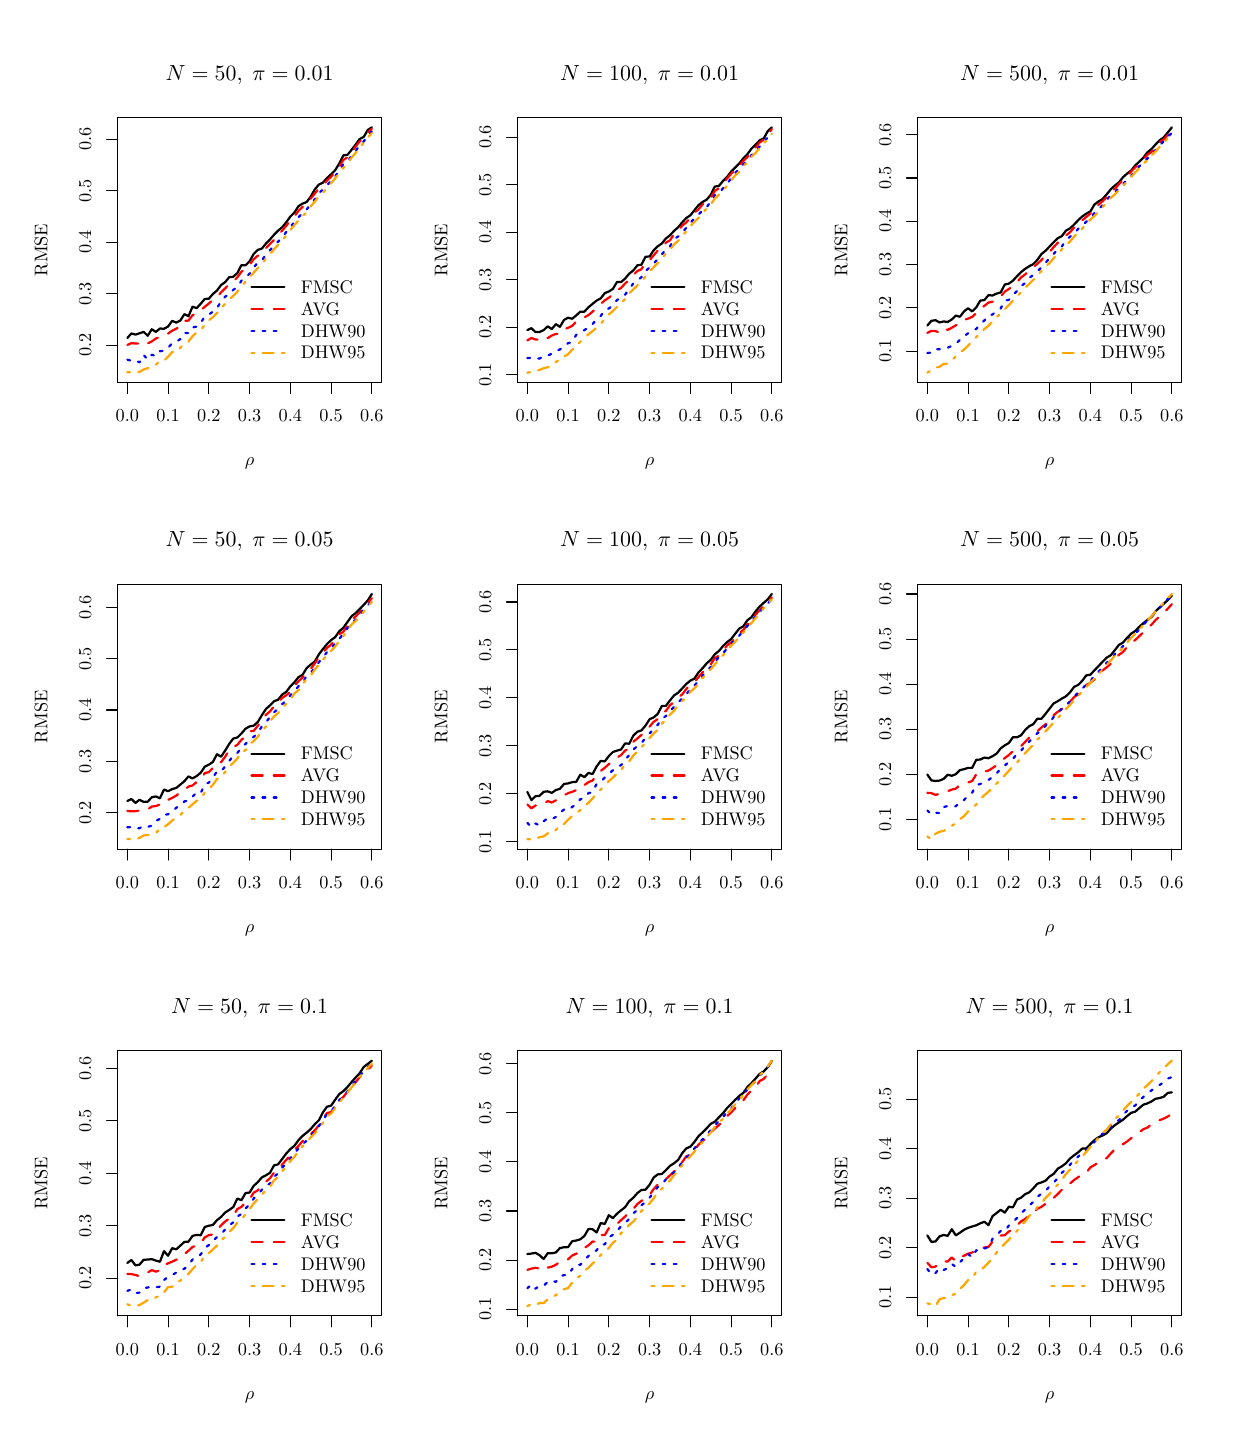
\begin{tikzpicture}[x=1pt,y=1pt]
\definecolor{fillColor}{RGB}{255,255,255}
\path[use as bounding box,fill=fillColor,fill opacity=0.00] (0,0) rectangle (433.62,505.89);
\begin{scope}
\path[clip] ( 32.47,377.65) rectangle (127.91,473.42);
\definecolor{drawColor}{RGB}{0,0,0}

\path[draw=drawColor,line width= 0.8pt,line join=round,line cap=round] ( 36.01,393.74) --
	( 37.48,395.40) --
	( 38.95,394.97) --
	( 40.42,395.45) --
	( 41.90,395.97) --
	( 43.37,394.55) --
	( 44.84,396.91) --
	( 46.32,395.96) --
	( 47.79,397.17) --
	( 49.26,397.09) --
	( 50.73,397.89) --
	( 52.21,399.93) --
	( 53.68,399.33) --
	( 55.15,400.04) --
	( 56.63,402.37) --
	( 58.10,401.61) --
	( 59.57,405.09) --
	( 61.04,404.51) --
	( 62.52,406.13) --
	( 63.99,407.86) --
	( 65.46,407.95) --
	( 66.93,409.64) --
	( 68.41,410.90) --
	( 69.88,412.90) --
	( 71.35,413.91) --
	( 72.83,415.74) --
	( 74.30,415.87) --
	( 75.77,417.22) --
	( 77.24,420.08) --
	( 78.72,420.02) --
	( 80.19,421.48) --
	( 81.66,424.11) --
	( 83.14,425.59) --
	( 84.61,426.04) --
	( 86.08,427.85) --
	( 87.55,429.35) --
	( 89.03,431.06) --
	( 90.50,432.55) --
	( 91.97,433.78) --
	( 93.44,435.57) --
	( 94.92,437.65) --
	( 96.39,439.12) --
	( 97.86,441.37) --
	( 99.34,442.32) --
	(100.81,442.88) --
	(102.28,444.83) --
	(103.75,447.45) --
	(105.23,449.19) --
	(106.70,449.92) --
	(108.17,451.56) --
	(109.65,452.92) --
	(111.12,454.41) --
	(112.59,456.80) --
	(114.06,459.74) --
	(115.54,459.92) --
	(117.01,461.72) --
	(118.48,463.61) --
	(119.95,465.63) --
	(121.43,466.42) --
	(122.90,468.94) --
	(124.37,469.87);
\end{scope}
\begin{scope}
\path[clip] (  0.00,  0.00) rectangle (433.62,505.89);
\definecolor{drawColor}{RGB}{0,0,0}

\path[draw=drawColor,line width= 0.4pt,line join=round,line cap=round] ( 36.01,377.65) -- (124.37,377.65);

\path[draw=drawColor,line width= 0.4pt,line join=round,line cap=round] ( 36.01,377.65) -- ( 36.01,373.69);

\path[draw=drawColor,line width= 0.4pt,line join=round,line cap=round] ( 50.73,377.65) -- ( 50.73,373.69);

\path[draw=drawColor,line width= 0.4pt,line join=round,line cap=round] ( 65.46,377.65) -- ( 65.46,373.69);

\path[draw=drawColor,line width= 0.4pt,line join=round,line cap=round] ( 80.19,377.65) -- ( 80.19,373.69);

\path[draw=drawColor,line width= 0.4pt,line join=round,line cap=round] ( 94.92,377.65) -- ( 94.92,373.69);

\path[draw=drawColor,line width= 0.4pt,line join=round,line cap=round] (109.65,377.65) -- (109.65,373.69);

\path[draw=drawColor,line width= 0.4pt,line join=round,line cap=round] (124.37,377.65) -- (124.37,373.69);

\node[text=drawColor,anchor=base,inner sep=0pt, outer sep=0pt, scale=  0.66] at ( 36.01,363.40) {0.0};

\node[text=drawColor,anchor=base,inner sep=0pt, outer sep=0pt, scale=  0.66] at ( 50.73,363.40) {0.1};

\node[text=drawColor,anchor=base,inner sep=0pt, outer sep=0pt, scale=  0.66] at ( 65.46,363.40) {0.2};

\node[text=drawColor,anchor=base,inner sep=0pt, outer sep=0pt, scale=  0.66] at ( 80.19,363.40) {0.3};

\node[text=drawColor,anchor=base,inner sep=0pt, outer sep=0pt, scale=  0.66] at ( 94.92,363.40) {0.4};

\node[text=drawColor,anchor=base,inner sep=0pt, outer sep=0pt, scale=  0.66] at (109.65,363.40) {0.5};

\node[text=drawColor,anchor=base,inner sep=0pt, outer sep=0pt, scale=  0.66] at (124.37,363.40) {0.6};

\path[draw=drawColor,line width= 0.4pt,line join=round,line cap=round] ( 32.47,391.13) -- ( 32.47,465.58);

\path[draw=drawColor,line width= 0.4pt,line join=round,line cap=round] ( 32.47,391.13) -- ( 28.51,391.13);

\path[draw=drawColor,line width= 0.4pt,line join=round,line cap=round] ( 32.47,409.74) -- ( 28.51,409.74);

\path[draw=drawColor,line width= 0.4pt,line join=round,line cap=round] ( 32.47,428.36) -- ( 28.51,428.36);

\path[draw=drawColor,line width= 0.4pt,line join=round,line cap=round] ( 32.47,446.97) -- ( 28.51,446.97);

\path[draw=drawColor,line width= 0.4pt,line join=round,line cap=round] ( 32.47,465.58) -- ( 28.51,465.58);

\node[text=drawColor,rotate= 90.00,anchor=base,inner sep=0pt, outer sep=0pt, scale=  0.66] at ( 22.97,391.13) {0.2};

\node[text=drawColor,rotate= 90.00,anchor=base,inner sep=0pt, outer sep=0pt, scale=  0.66] at ( 22.97,409.74) {0.3};

\node[text=drawColor,rotate= 90.00,anchor=base,inner sep=0pt, outer sep=0pt, scale=  0.66] at ( 22.97,428.36) {0.4};

\node[text=drawColor,rotate= 90.00,anchor=base,inner sep=0pt, outer sep=0pt, scale=  0.66] at ( 22.97,446.97) {0.5};

\node[text=drawColor,rotate= 90.00,anchor=base,inner sep=0pt, outer sep=0pt, scale=  0.66] at ( 22.97,465.58) {0.6};

\path[draw=drawColor,line width= 0.4pt,line join=round,line cap=round] ( 32.47,377.65) --
	(127.91,377.65) --
	(127.91,473.42) --
	( 32.47,473.42) --
	( 32.47,377.65);
\end{scope}
\begin{scope}
\path[clip] (  0.00,337.26) rectangle (144.54,505.89);
\definecolor{drawColor}{RGB}{0,0,0}

\node[text=drawColor,anchor=base,inner sep=0pt, outer sep=0pt, scale=  0.79] at ( 80.19,486.92) {\bfseries $N=50, \;\pi=0.01$};

\node[text=drawColor,anchor=base,inner sep=0pt, outer sep=0pt, scale=  0.66] at ( 80.19,347.56) {$\rho$};

\node[text=drawColor,rotate= 90.00,anchor=base,inner sep=0pt, outer sep=0pt, scale=  0.66] at (  7.13,425.53) {RMSE};
\end{scope}
\begin{scope}
\path[clip] ( 32.47,377.65) rectangle (127.91,473.42);
\definecolor{drawColor}{RGB}{255,0,0}

\path[draw=drawColor,line width= 0.8pt,dash pattern=on 4pt off 4pt ,line join=round,line cap=round] ( 36.01,391.24) --
	( 37.48,391.90) --
	( 38.95,391.73) --
	( 40.42,391.79) --
	( 41.90,392.47) --
	( 43.37,391.80) --
	( 44.84,392.50) --
	( 46.32,393.56) --
	( 47.79,394.16) --
	( 49.26,394.63) --
	( 50.73,395.35) --
	( 52.21,396.39) --
	( 53.68,397.11) --
	( 55.15,397.91) --
	( 56.63,399.94) --
	( 58.10,400.04) --
	( 59.57,401.99) --
	( 61.04,402.50) --
	( 62.52,403.67) --
	( 63.99,405.04) --
	( 65.46,406.22) --
	( 66.93,407.51) --
	( 68.41,408.50) --
	( 69.88,410.25) --
	( 71.35,411.65) --
	( 72.83,413.35) --
	( 74.30,414.22) --
	( 75.77,415.68) --
	( 77.24,417.71) --
	( 78.72,418.65) --
	( 80.19,420.20) --
	( 81.66,422.18) --
	( 83.14,423.47) --
	( 84.61,424.42) --
	( 86.08,426.19) --
	( 87.55,427.73) --
	( 89.03,429.20) --
	( 90.50,430.84) --
	( 91.97,432.58) --
	( 93.44,434.29) --
	( 94.92,436.32) --
	( 96.39,437.76) --
	( 97.86,439.70) --
	( 99.34,441.11) --
	(100.81,442.19) --
	(102.28,444.17) --
	(103.75,445.97) --
	(105.23,447.78) --
	(106.70,448.91) --
	(108.17,450.66) --
	(109.65,452.03) --
	(111.12,453.83) --
	(112.59,455.76) --
	(114.06,458.10) --
	(115.54,458.99) --
	(117.01,460.83) --
	(118.48,462.88) --
	(119.95,464.77) --
	(121.43,465.74) --
	(122.90,468.03) --
	(124.37,469.39);
\definecolor{drawColor}{RGB}{0,0,255}

\path[draw=drawColor,line width= 0.8pt,dash pattern=on 1pt off 3pt ,line join=round,line cap=round] ( 36.01,385.91) --
	( 37.48,385.53) --
	( 38.95,385.65) --
	( 40.42,384.94) --
	( 41.90,387.63) --
	( 43.37,385.90) --
	( 44.84,387.68) --
	( 46.32,387.28) --
	( 47.79,388.99) --
	( 49.26,389.07) --
	( 50.73,390.26) --
	( 52.21,391.84) --
	( 53.68,392.34) --
	( 55.15,393.35) --
	( 56.63,395.63) --
	( 58.10,395.52) --
	( 59.57,397.57) --
	( 61.04,397.86) --
	( 62.52,399.15) --
	( 63.99,401.53) --
	( 65.46,402.16) --
	( 66.93,403.33) --
	( 68.41,404.45) --
	( 69.88,407.08) --
	( 71.35,408.69) --
	( 72.83,409.52) --
	( 74.30,411.16) --
	( 75.77,412.10) --
	( 77.24,414.45) --
	( 78.72,415.62) --
	( 80.19,417.00) --
	( 81.66,419.18) --
	( 83.14,421.03) --
	( 84.61,421.79) --
	( 86.08,423.83) --
	( 87.55,425.44) --
	( 89.03,427.14) --
	( 90.50,428.55) --
	( 91.97,430.23) --
	( 93.44,432.03) --
	( 94.92,433.91) --
	( 96.39,435.59) --
	( 97.86,437.42) --
	( 99.34,438.79) --
	(100.81,440.17) --
	(102.28,442.23) --
	(103.75,443.84) --
	(105.23,446.17) --
	(106.70,447.36) --
	(108.17,448.87) --
	(109.65,450.62) --
	(111.12,452.18) --
	(112.59,454.28) --
	(114.06,456.61) --
	(115.54,457.49) --
	(117.01,459.55) --
	(118.48,461.28) --
	(119.95,463.36) --
	(121.43,464.77) --
	(122.90,466.97) --
	(124.37,468.41);
\definecolor{drawColor}{RGB}{255,165,0}

\path[draw=drawColor,line width= 0.8pt,dash pattern=on 1pt off 3pt on 4pt off 3pt ,line join=round,line cap=round] ( 36.01,381.38) --
	( 37.48,381.38) --
	( 38.95,381.20) --
	( 40.42,381.51) --
	( 41.90,382.38) --
	( 43.37,382.84) --
	( 44.84,383.16) --
	( 46.32,384.09) --
	( 47.79,385.47) --
	( 49.26,385.60) --
	( 50.73,387.01) --
	( 52.21,388.68) --
	( 53.68,388.74) --
	( 55.15,390.23) --
	( 56.63,391.66) --
	( 58.10,392.47) --
	( 59.57,394.39) --
	( 61.04,395.76) --
	( 62.52,396.60) --
	( 63.99,398.48) --
	( 65.46,400.14) --
	( 66.93,401.26) --
	( 68.41,402.79) --
	( 69.88,404.52) --
	( 71.35,406.09) --
	( 72.83,407.67) --
	( 74.30,408.97) --
	( 75.77,410.47) --
	( 77.24,412.52) --
	( 78.72,414.08) --
	( 80.19,415.67) --
	( 81.66,417.36) --
	( 83.14,419.03) --
	( 84.61,420.38) --
	( 86.08,422.46) --
	( 87.55,423.98) --
	( 89.03,425.82) --
	( 90.50,427.43) --
	( 91.97,429.12) --
	( 93.44,430.72) --
	( 94.92,432.75) --
	( 96.39,434.57) --
	( 97.86,436.21) --
	( 99.34,437.83) --
	(100.81,439.14) --
	(102.28,441.33) --
	(103.75,443.07) --
	(105.23,444.99) --
	(106.70,446.21) --
	(108.17,448.13) --
	(109.65,449.73) --
	(111.12,451.45) --
	(112.59,453.39) --
	(114.06,455.21) --
	(115.54,456.71) --
	(117.01,458.95) --
	(118.48,460.55) --
	(119.95,462.61) --
	(121.43,464.24) --
	(122.90,466.26) --
	(124.37,467.81);
\definecolor{drawColor}{RGB}{0,0,0}

\path[draw=drawColor,line width= 0.8pt,line join=round,line cap=round] ( 80.89,412.20) -- ( 92.77,412.20);
\definecolor{drawColor}{RGB}{255,0,0}

\path[draw=drawColor,line width= 0.8pt,dash pattern=on 4pt off 4pt ,line join=round,line cap=round] ( 80.89,404.28) -- ( 92.77,404.28);
\definecolor{drawColor}{RGB}{0,0,255}

\path[draw=drawColor,line width= 0.8pt,dash pattern=on 1pt off 3pt ,line join=round,line cap=round] ( 80.89,396.36) -- ( 92.77,396.36);
\definecolor{drawColor}{RGB}{255,165,0}

\path[draw=drawColor,line width= 0.8pt,dash pattern=on 1pt off 3pt on 4pt off 3pt ,line join=round,line cap=round] ( 80.89,388.44) -- ( 92.77,388.44);
\definecolor{drawColor}{RGB}{0,0,0}

\node[text=drawColor,anchor=base west,inner sep=0pt, outer sep=0pt, scale=  0.66] at ( 98.71,409.93) {FMSC};

\node[text=drawColor,anchor=base west,inner sep=0pt, outer sep=0pt, scale=  0.66] at ( 98.71,402.01) {AVG};

\node[text=drawColor,anchor=base west,inner sep=0pt, outer sep=0pt, scale=  0.66] at ( 98.71,394.09) {DHW90};

\node[text=drawColor,anchor=base west,inner sep=0pt, outer sep=0pt, scale=  0.66] at ( 98.71,386.17) {DHW95};
\end{scope}
\begin{scope}
\path[clip] (177.01,377.65) rectangle (272.45,473.42);
\definecolor{drawColor}{RGB}{0,0,0}

\path[draw=drawColor,line width= 0.8pt,line join=round,line cap=round] (180.55,396.61) --
	(182.02,397.30) --
	(183.49,395.89) --
	(184.96,395.91) --
	(186.44,396.59) --
	(187.91,397.95) --
	(189.38,396.98) --
	(190.86,398.75) --
	(192.33,397.77) --
	(193.80,400.28) --
	(195.27,401.07) --
	(196.75,400.70) --
	(198.22,401.92) --
	(199.69,403.26) --
	(201.17,403.27) --
	(202.64,404.85) --
	(204.11,406.08) --
	(205.58,407.26) --
	(207.06,408.06) --
	(208.53,409.96) --
	(210.00,410.55) --
	(211.47,411.50) --
	(212.95,413.99) --
	(214.42,413.95) --
	(215.89,415.22) --
	(217.37,416.99) --
	(218.84,418.15) --
	(220.31,420.00) --
	(221.78,420.24) --
	(223.26,423.11) --
	(224.73,423.19) --
	(226.20,425.44) --
	(227.68,426.90) --
	(229.15,427.89) --
	(230.62,429.71) --
	(232.09,430.84) --
	(233.57,432.46) --
	(235.04,433.75) --
	(236.51,435.53) --
	(237.98,437.10) --
	(239.46,438.07) --
	(240.93,439.91) --
	(242.40,441.75) --
	(243.88,442.91) --
	(245.35,443.73) --
	(246.82,445.49) --
	(248.29,448.48) --
	(249.77,448.68) --
	(251.24,450.48) --
	(252.71,451.94) --
	(254.19,453.87) --
	(255.66,455.35) --
	(257.13,456.82) --
	(258.60,458.69) --
	(260.08,460.17) --
	(261.55,462.18) --
	(263.02,463.58) --
	(264.50,465.17) --
	(265.97,465.85) --
	(267.44,468.50) --
	(268.91,469.87);
\end{scope}
\begin{scope}
\path[clip] (  0.00,  0.00) rectangle (433.62,505.89);
\definecolor{drawColor}{RGB}{0,0,0}

\path[draw=drawColor,line width= 0.4pt,line join=round,line cap=round] (180.55,377.65) -- (268.91,377.65);

\path[draw=drawColor,line width= 0.4pt,line join=round,line cap=round] (180.55,377.65) -- (180.55,373.69);

\path[draw=drawColor,line width= 0.4pt,line join=round,line cap=round] (195.27,377.65) -- (195.27,373.69);

\path[draw=drawColor,line width= 0.4pt,line join=round,line cap=round] (210.00,377.65) -- (210.00,373.69);

\path[draw=drawColor,line width= 0.4pt,line join=round,line cap=round] (224.73,377.65) -- (224.73,373.69);

\path[draw=drawColor,line width= 0.4pt,line join=round,line cap=round] (239.46,377.65) -- (239.46,373.69);

\path[draw=drawColor,line width= 0.4pt,line join=round,line cap=round] (254.19,377.65) -- (254.19,373.69);

\path[draw=drawColor,line width= 0.4pt,line join=round,line cap=round] (268.91,377.65) -- (268.91,373.69);

\node[text=drawColor,anchor=base,inner sep=0pt, outer sep=0pt, scale=  0.66] at (180.55,363.40) {0.0};

\node[text=drawColor,anchor=base,inner sep=0pt, outer sep=0pt, scale=  0.66] at (195.27,363.40) {0.1};

\node[text=drawColor,anchor=base,inner sep=0pt, outer sep=0pt, scale=  0.66] at (210.00,363.40) {0.2};

\node[text=drawColor,anchor=base,inner sep=0pt, outer sep=0pt, scale=  0.66] at (224.73,363.40) {0.3};

\node[text=drawColor,anchor=base,inner sep=0pt, outer sep=0pt, scale=  0.66] at (239.46,363.40) {0.4};

\node[text=drawColor,anchor=base,inner sep=0pt, outer sep=0pt, scale=  0.66] at (254.19,363.40) {0.5};

\node[text=drawColor,anchor=base,inner sep=0pt, outer sep=0pt, scale=  0.66] at (268.91,363.40) {0.6};

\path[draw=drawColor,line width= 0.4pt,line join=round,line cap=round] (177.01,380.55) -- (177.01,466.31);

\path[draw=drawColor,line width= 0.4pt,line join=round,line cap=round] (177.01,380.55) -- (173.05,380.55);

\path[draw=drawColor,line width= 0.4pt,line join=round,line cap=round] (177.01,397.70) -- (173.05,397.70);

\path[draw=drawColor,line width= 0.4pt,line join=round,line cap=round] (177.01,414.85) -- (173.05,414.85);

\path[draw=drawColor,line width= 0.4pt,line join=round,line cap=round] (177.01,432.01) -- (173.05,432.01);

\path[draw=drawColor,line width= 0.4pt,line join=round,line cap=round] (177.01,449.16) -- (173.05,449.16);

\path[draw=drawColor,line width= 0.4pt,line join=round,line cap=round] (177.01,466.31) -- (173.05,466.31);

\node[text=drawColor,rotate= 90.00,anchor=base,inner sep=0pt, outer sep=0pt, scale=  0.66] at (167.51,380.55) {0.1};

\node[text=drawColor,rotate= 90.00,anchor=base,inner sep=0pt, outer sep=0pt, scale=  0.66] at (167.51,397.70) {0.2};

\node[text=drawColor,rotate= 90.00,anchor=base,inner sep=0pt, outer sep=0pt, scale=  0.66] at (167.51,414.85) {0.3};

\node[text=drawColor,rotate= 90.00,anchor=base,inner sep=0pt, outer sep=0pt, scale=  0.66] at (167.51,432.01) {0.4};

\node[text=drawColor,rotate= 90.00,anchor=base,inner sep=0pt, outer sep=0pt, scale=  0.66] at (167.51,449.16) {0.5};

\node[text=drawColor,rotate= 90.00,anchor=base,inner sep=0pt, outer sep=0pt, scale=  0.66] at (167.51,466.31) {0.6};

\path[draw=drawColor,line width= 0.4pt,line join=round,line cap=round] (177.01,377.65) --
	(272.45,377.65) --
	(272.45,473.42) --
	(177.01,473.42) --
	(177.01,377.65);
\end{scope}
\begin{scope}
\path[clip] (144.54,337.26) rectangle (289.08,505.89);
\definecolor{drawColor}{RGB}{0,0,0}

\node[text=drawColor,anchor=base,inner sep=0pt, outer sep=0pt, scale=  0.79] at (224.73,486.92) {\bfseries $N=100, \;\pi=0.01$};

\node[text=drawColor,anchor=base,inner sep=0pt, outer sep=0pt, scale=  0.66] at (224.73,347.56) {$\rho$};

\node[text=drawColor,rotate= 90.00,anchor=base,inner sep=0pt, outer sep=0pt, scale=  0.66] at (151.67,425.53) {RMSE};
\end{scope}
\begin{scope}
\path[clip] (177.01,377.65) rectangle (272.45,473.42);
\definecolor{drawColor}{RGB}{255,0,0}

\path[draw=drawColor,line width= 0.8pt,dash pattern=on 4pt off 4pt ,line join=round,line cap=round] (180.55,392.86) --
	(182.02,393.75) --
	(183.49,393.21) --
	(184.96,393.09) --
	(186.44,394.13) --
	(187.91,393.71) --
	(189.38,394.64) --
	(190.86,395.22) --
	(192.33,395.25) --
	(193.80,396.84) --
	(195.27,397.43) --
	(196.75,398.12) --
	(198.22,399.69) --
	(199.69,400.22) --
	(201.17,401.21) --
	(202.64,402.04) --
	(204.11,403.28) --
	(205.58,404.49) --
	(207.06,406.04) --
	(208.53,407.37) --
	(210.00,408.31) --
	(211.47,409.47) --
	(212.95,411.00) --
	(214.42,411.84) --
	(215.89,413.47) --
	(217.37,414.79) --
	(218.84,416.45) --
	(220.31,417.95) --
	(221.78,418.59) --
	(223.26,421.29) --
	(224.73,421.90) --
	(226.20,423.62) --
	(227.68,425.31) --
	(229.15,426.09) --
	(230.62,428.23) --
	(232.09,429.03) --
	(233.57,431.25) --
	(235.04,432.48) --
	(236.51,434.34) --
	(237.98,435.52) --
	(239.46,437.14) --
	(240.93,439.05) --
	(242.40,440.22) --
	(243.88,442.05) --
	(245.35,442.75) --
	(246.82,444.51) --
	(248.29,446.85) --
	(249.77,447.84) --
	(251.24,449.55) --
	(252.71,451.37) --
	(254.19,453.10) --
	(255.66,454.48) --
	(257.13,456.06) --
	(258.60,457.73) --
	(260.08,459.13) --
	(261.55,461.18) --
	(263.02,462.54) --
	(264.50,464.42) --
	(265.97,465.38) --
	(267.44,467.41) --
	(268.91,469.22);
\definecolor{drawColor}{RGB}{0,0,255}

\path[draw=drawColor,line width= 0.8pt,dash pattern=on 1pt off 3pt ,line join=round,line cap=round] (180.55,386.51) --
	(182.02,386.56) --
	(183.49,386.28) --
	(184.96,386.32) --
	(186.44,387.09) --
	(187.91,387.34) --
	(189.38,388.08) --
	(190.86,389.18) --
	(192.33,389.58) --
	(193.80,390.84) --
	(195.27,391.85) --
	(196.75,392.34) --
	(198.22,394.89) --
	(199.69,395.78) --
	(201.17,396.60) --
	(202.64,397.54) --
	(204.11,398.73) --
	(205.58,400.58) --
	(207.06,401.70) --
	(208.53,403.81) --
	(210.00,404.42) --
	(211.47,405.54) --
	(212.95,407.46) --
	(214.42,408.39) --
	(215.89,409.43) --
	(217.37,411.43) --
	(218.84,413.45) --
	(220.31,414.52) --
	(221.78,415.72) --
	(223.26,417.94) --
	(224.73,419.23) --
	(226.20,420.60) --
	(227.68,422.34) --
	(229.15,423.91) --
	(230.62,425.84) --
	(232.09,426.83) --
	(233.57,429.46) --
	(235.04,430.43) --
	(236.51,431.81) --
	(237.98,433.57) --
	(239.46,435.38) --
	(240.93,436.95) --
	(242.40,438.35) --
	(243.88,439.90) --
	(245.35,441.02) --
	(246.82,443.07) --
	(248.29,445.35) --
	(249.77,446.08) --
	(251.24,447.82) --
	(252.71,449.41) --
	(254.19,451.55) --
	(255.66,453.45) --
	(257.13,454.71) --
	(258.60,456.47) --
	(260.08,457.96) --
	(261.55,459.80) --
	(263.02,461.33) --
	(264.50,462.92) --
	(265.97,464.43) --
	(267.44,466.36) --
	(268.91,468.02);
\definecolor{drawColor}{RGB}{255,165,0}

\path[draw=drawColor,line width= 0.8pt,dash pattern=on 1pt off 3pt on 4pt off 3pt ,line join=round,line cap=round] (180.55,381.20) --
	(182.02,381.50) --
	(183.49,381.89) --
	(184.96,382.24) --
	(186.44,382.83) --
	(187.91,383.19) --
	(189.38,384.19) --
	(190.86,385.05) --
	(192.33,385.96) --
	(193.80,387.07) --
	(195.27,387.86) --
	(196.75,389.52) --
	(198.22,390.94) --
	(199.69,392.37) --
	(201.17,393.56) --
	(202.64,395.09) --
	(204.11,396.19) --
	(205.58,397.52) --
	(207.06,398.92) --
	(208.53,400.58) --
	(210.00,402.23) --
	(211.47,403.53) --
	(212.95,405.00) --
	(214.42,406.23) --
	(215.89,407.94) --
	(217.37,409.83) --
	(218.84,411.35) --
	(220.31,412.71) --
	(221.78,414.11) --
	(223.26,416.04) --
	(224.73,417.78) --
	(226.20,419.35) --
	(227.68,420.84) --
	(229.15,422.56) --
	(230.62,424.30) --
	(232.09,425.65) --
	(233.57,427.60) --
	(235.04,428.84) --
	(236.51,430.66) --
	(237.98,432.30) --
	(239.46,434.15) --
	(240.93,435.71) --
	(242.40,437.15) --
	(243.88,439.04) --
	(245.35,440.48) --
	(246.82,441.96) --
	(248.29,444.13) --
	(249.77,445.52) --
	(251.24,447.23) --
	(252.71,448.69) --
	(254.19,450.70) --
	(255.66,452.51) --
	(257.13,453.87) --
	(258.60,455.79) --
	(260.08,457.33) --
	(261.55,459.28) --
	(263.02,460.60) --
	(264.50,462.41) --
	(265.97,464.00) --
	(267.44,465.66) --
	(268.91,467.49);
\definecolor{drawColor}{RGB}{0,0,0}

\path[draw=drawColor,line width= 0.8pt,line join=round,line cap=round] (225.43,412.20) -- (237.31,412.20);
\definecolor{drawColor}{RGB}{255,0,0}

\path[draw=drawColor,line width= 0.8pt,dash pattern=on 4pt off 4pt ,line join=round,line cap=round] (225.43,404.28) -- (237.31,404.28);
\definecolor{drawColor}{RGB}{0,0,255}

\path[draw=drawColor,line width= 0.8pt,dash pattern=on 1pt off 3pt ,line join=round,line cap=round] (225.43,396.36) -- (237.31,396.36);
\definecolor{drawColor}{RGB}{255,165,0}

\path[draw=drawColor,line width= 0.8pt,dash pattern=on 1pt off 3pt on 4pt off 3pt ,line join=round,line cap=round] (225.43,388.44) -- (237.31,388.44);
\definecolor{drawColor}{RGB}{0,0,0}

\node[text=drawColor,anchor=base west,inner sep=0pt, outer sep=0pt, scale=  0.66] at (243.25,409.93) {FMSC};

\node[text=drawColor,anchor=base west,inner sep=0pt, outer sep=0pt, scale=  0.66] at (243.25,402.01) {AVG};

\node[text=drawColor,anchor=base west,inner sep=0pt, outer sep=0pt, scale=  0.66] at (243.25,394.09) {DHW90};

\node[text=drawColor,anchor=base west,inner sep=0pt, outer sep=0pt, scale=  0.66] at (243.25,386.17) {DHW95};
\end{scope}
\begin{scope}
\path[clip] (321.55,377.65) rectangle (416.99,473.42);
\definecolor{drawColor}{RGB}{0,0,0}

\path[draw=drawColor,line width= 0.8pt,line join=round,line cap=round] (325.09,398.24) --
	(326.56,399.95) --
	(328.03,400.18) --
	(329.50,399.37) --
	(330.98,399.73) --
	(332.45,399.55) --
	(333.92,400.43) --
	(335.40,401.85) --
	(336.87,401.41) --
	(338.34,403.35) --
	(339.81,404.50) --
	(341.29,403.36) --
	(342.76,404.79) --
	(344.23,407.27) --
	(345.71,407.45) --
	(347.18,409.22) --
	(348.65,409.11) --
	(350.12,409.79) --
	(351.60,410.21) --
	(353.07,413.07) --
	(354.54,413.40) --
	(356.01,414.46) --
	(357.49,416.06) --
	(358.96,417.56) --
	(360.43,418.74) --
	(361.91,419.69) --
	(363.38,420.44) --
	(364.85,421.96) --
	(366.32,424.08) --
	(367.80,425.28) --
	(369.27,426.81) --
	(370.74,428.37) --
	(372.22,429.79) --
	(373.69,430.56) --
	(375.16,432.52) --
	(376.63,433.35) --
	(378.11,434.72) --
	(379.58,436.31) --
	(381.05,437.65) --
	(382.52,438.67) --
	(384.00,439.47) --
	(385.47,441.97) --
	(386.94,443.08) --
	(388.42,443.95) --
	(389.89,445.65) --
	(391.36,447.48) --
	(392.83,448.81) --
	(394.31,449.96) --
	(395.78,451.83) --
	(397.25,453.13) --
	(398.73,454.24) --
	(400.20,456.09) --
	(401.67,457.46) --
	(403.14,458.88) --
	(404.62,460.86) --
	(406.09,462.02) --
	(407.56,463.68) --
	(409.04,465.18) --
	(410.51,466.24) --
	(411.98,468.01) --
	(413.45,469.87);
\end{scope}
\begin{scope}
\path[clip] (  0.00,  0.00) rectangle (433.62,505.89);
\definecolor{drawColor}{RGB}{0,0,0}

\path[draw=drawColor,line width= 0.4pt,line join=round,line cap=round] (325.09,377.65) -- (413.45,377.65);

\path[draw=drawColor,line width= 0.4pt,line join=round,line cap=round] (325.09,377.65) -- (325.09,373.69);

\path[draw=drawColor,line width= 0.4pt,line join=round,line cap=round] (339.81,377.65) -- (339.81,373.69);

\path[draw=drawColor,line width= 0.4pt,line join=round,line cap=round] (354.54,377.65) -- (354.54,373.69);

\path[draw=drawColor,line width= 0.4pt,line join=round,line cap=round] (369.27,377.65) -- (369.27,373.69);

\path[draw=drawColor,line width= 0.4pt,line join=round,line cap=round] (384.00,377.65) -- (384.00,373.69);

\path[draw=drawColor,line width= 0.4pt,line join=round,line cap=round] (398.73,377.65) -- (398.73,373.69);

\path[draw=drawColor,line width= 0.4pt,line join=round,line cap=round] (413.45,377.65) -- (413.45,373.69);

\node[text=drawColor,anchor=base,inner sep=0pt, outer sep=0pt, scale=  0.66] at (325.09,363.40) {0.0};

\node[text=drawColor,anchor=base,inner sep=0pt, outer sep=0pt, scale=  0.66] at (339.81,363.40) {0.1};

\node[text=drawColor,anchor=base,inner sep=0pt, outer sep=0pt, scale=  0.66] at (354.54,363.40) {0.2};

\node[text=drawColor,anchor=base,inner sep=0pt, outer sep=0pt, scale=  0.66] at (369.27,363.40) {0.3};

\node[text=drawColor,anchor=base,inner sep=0pt, outer sep=0pt, scale=  0.66] at (384.00,363.40) {0.4};

\node[text=drawColor,anchor=base,inner sep=0pt, outer sep=0pt, scale=  0.66] at (398.73,363.40) {0.5};

\node[text=drawColor,anchor=base,inner sep=0pt, outer sep=0pt, scale=  0.66] at (413.45,363.40) {0.6};

\path[draw=drawColor,line width= 0.4pt,line join=round,line cap=round] (321.55,389.03) -- (321.55,467.21);

\path[draw=drawColor,line width= 0.4pt,line join=round,line cap=round] (321.55,389.03) -- (317.59,389.03);

\path[draw=drawColor,line width= 0.4pt,line join=round,line cap=round] (321.55,404.67) -- (317.59,404.67);

\path[draw=drawColor,line width= 0.4pt,line join=round,line cap=round] (321.55,420.30) -- (317.59,420.30);

\path[draw=drawColor,line width= 0.4pt,line join=round,line cap=round] (321.55,435.94) -- (317.59,435.94);

\path[draw=drawColor,line width= 0.4pt,line join=round,line cap=round] (321.55,451.58) -- (317.59,451.58);

\path[draw=drawColor,line width= 0.4pt,line join=round,line cap=round] (321.55,467.21) -- (317.59,467.21);

\node[text=drawColor,rotate= 90.00,anchor=base,inner sep=0pt, outer sep=0pt, scale=  0.66] at (312.05,389.03) {0.1};

\node[text=drawColor,rotate= 90.00,anchor=base,inner sep=0pt, outer sep=0pt, scale=  0.66] at (312.05,404.67) {0.2};

\node[text=drawColor,rotate= 90.00,anchor=base,inner sep=0pt, outer sep=0pt, scale=  0.66] at (312.05,420.30) {0.3};

\node[text=drawColor,rotate= 90.00,anchor=base,inner sep=0pt, outer sep=0pt, scale=  0.66] at (312.05,435.94) {0.4};

\node[text=drawColor,rotate= 90.00,anchor=base,inner sep=0pt, outer sep=0pt, scale=  0.66] at (312.05,451.58) {0.5};

\node[text=drawColor,rotate= 90.00,anchor=base,inner sep=0pt, outer sep=0pt, scale=  0.66] at (312.05,467.21) {0.6};

\path[draw=drawColor,line width= 0.4pt,line join=round,line cap=round] (321.55,377.65) --
	(416.99,377.65) --
	(416.99,473.42) --
	(321.55,473.42) --
	(321.55,377.65);
\end{scope}
\begin{scope}
\path[clip] (289.08,337.26) rectangle (433.62,505.89);
\definecolor{drawColor}{RGB}{0,0,0}

\node[text=drawColor,anchor=base,inner sep=0pt, outer sep=0pt, scale=  0.79] at (369.27,486.92) {\bfseries $N=500, \;\pi=0.01$};

\node[text=drawColor,anchor=base,inner sep=0pt, outer sep=0pt, scale=  0.66] at (369.27,347.56) {$\rho$};

\node[text=drawColor,rotate= 90.00,anchor=base,inner sep=0pt, outer sep=0pt, scale=  0.66] at (296.21,425.53) {RMSE};
\end{scope}
\begin{scope}
\path[clip] (321.55,377.65) rectangle (416.99,473.42);
\definecolor{drawColor}{RGB}{255,0,0}

\path[draw=drawColor,line width= 0.8pt,dash pattern=on 4pt off 4pt ,line join=round,line cap=round] (325.09,395.58) --
	(326.56,396.31) --
	(328.03,396.21) --
	(329.50,395.77) --
	(330.98,397.30) --
	(332.45,396.70) --
	(333.92,397.44) --
	(335.40,398.36) --
	(336.87,398.89) --
	(338.34,400.24) --
	(339.81,400.76) --
	(341.29,401.38) --
	(342.76,402.72) --
	(344.23,404.44) --
	(345.71,405.35) --
	(347.18,406.55) --
	(348.65,406.87) --
	(350.12,408.00) --
	(351.60,408.79) --
	(353.07,410.48) --
	(354.54,411.47) --
	(356.01,412.48) --
	(357.49,413.89) --
	(358.96,415.66) --
	(360.43,416.71) --
	(361.91,418.24) --
	(363.38,419.32) --
	(364.85,420.55) --
	(366.32,421.91) --
	(367.80,423.68) --
	(369.27,424.85) --
	(370.74,426.59) --
	(372.22,428.18) --
	(373.69,429.21) --
	(375.16,430.77) --
	(376.63,431.96) --
	(378.11,433.65) --
	(379.58,435.26) --
	(381.05,436.24) --
	(382.52,437.50) --
	(384.00,438.73) --
	(385.47,440.92) --
	(386.94,441.93) --
	(388.42,443.16) --
	(389.89,444.71) --
	(391.36,446.54) --
	(392.83,447.62) --
	(394.31,449.35) --
	(395.78,450.86) --
	(397.25,452.14) --
	(398.73,453.91) --
	(400.20,455.37) --
	(401.67,456.83) --
	(403.14,458.23) --
	(404.62,459.96) --
	(406.09,461.00) --
	(407.56,462.91) --
	(409.04,464.48) --
	(410.51,465.54) --
	(411.98,467.18) --
	(413.45,469.05);
\definecolor{drawColor}{RGB}{0,0,255}

\path[draw=drawColor,line width= 0.8pt,dash pattern=on 1pt off 3pt ,line join=round,line cap=round] (325.09,388.31) --
	(326.56,388.49) --
	(328.03,389.72) --
	(329.50,389.68) --
	(330.98,390.10) --
	(332.45,390.25) --
	(333.92,390.91) --
	(335.40,391.73) --
	(336.87,393.07) --
	(338.34,394.34) --
	(339.81,395.46) --
	(341.29,396.45) --
	(342.76,397.03) --
	(344.23,398.73) --
	(345.71,400.10) --
	(347.18,401.87) --
	(348.65,402.25) --
	(350.12,403.53) --
	(351.60,404.42) --
	(353.07,407.22) --
	(354.54,407.55) --
	(356.01,409.20) --
	(357.49,410.75) --
	(358.96,412.54) --
	(360.43,413.61) --
	(361.91,415.39) --
	(363.38,416.60) --
	(364.85,417.83) --
	(366.32,419.31) --
	(367.80,420.96) --
	(369.27,422.58) --
	(370.74,424.13) --
	(372.22,425.80) --
	(373.69,426.86) --
	(375.16,428.92) --
	(376.63,430.35) --
	(378.11,431.37) --
	(379.58,433.18) --
	(381.05,434.26) --
	(382.52,435.78) --
	(384.00,437.12) --
	(385.47,438.93) --
	(386.94,440.21) --
	(388.42,441.77) --
	(389.89,443.68) --
	(391.36,445.29) --
	(392.83,446.20) --
	(394.31,448.05) --
	(395.78,449.32) --
	(397.25,451.00) --
	(398.73,452.34) --
	(400.20,454.05) --
	(401.67,455.82) --
	(403.14,457.14) --
	(404.62,458.60) --
	(406.09,460.32) --
	(407.56,461.64) --
	(409.04,463.45) --
	(410.51,464.77) --
	(411.98,466.51) --
	(413.45,467.83);
\definecolor{drawColor}{RGB}{255,165,0}

\path[draw=drawColor,line width= 0.8pt,dash pattern=on 1pt off 3pt on 4pt off 3pt ,line join=round,line cap=round] (325.09,381.20) --
	(326.56,382.20) --
	(328.03,383.01) --
	(329.50,383.37) --
	(330.98,384.36) --
	(332.45,384.50) --
	(333.92,385.54) --
	(335.40,387.24) --
	(336.87,388.53) --
	(338.34,389.58) --
	(339.81,390.99) --
	(341.29,392.57) --
	(342.76,394.07) --
	(344.23,395.39) --
	(345.71,397.04) --
	(347.18,398.12) --
	(348.65,399.74) --
	(350.12,401.35) --
	(351.60,402.59) --
	(353.07,404.18) --
	(354.54,405.64) --
	(356.01,407.22) --
	(357.49,408.73) --
	(358.96,410.30) --
	(360.43,411.87) --
	(361.91,413.31) --
	(363.38,414.77) --
	(364.85,416.26) --
	(366.32,418.00) --
	(367.80,419.57) --
	(369.27,420.84) --
	(370.74,422.59) --
	(372.22,424.04) --
	(373.69,425.76) --
	(375.16,427.16) --
	(376.63,428.62) --
	(378.11,430.33) --
	(379.58,431.93) --
	(381.05,433.29) --
	(382.52,434.94) --
	(384.00,436.53) --
	(385.47,437.88) --
	(386.94,439.45) --
	(388.42,441.09) --
	(389.89,442.72) --
	(391.36,444.41) --
	(392.83,445.64) --
	(394.31,447.17) --
	(395.78,448.71) --
	(397.25,450.30) --
	(398.73,451.97) --
	(400.20,453.58) --
	(401.67,455.11) --
	(403.14,456.64) --
	(404.62,458.11) --
	(406.09,459.64) --
	(407.56,461.16) --
	(409.04,462.87) --
	(410.51,464.35) --
	(411.98,465.92) --
	(413.45,467.37);
\definecolor{drawColor}{RGB}{0,0,0}

\path[draw=drawColor,line width= 0.8pt,line join=round,line cap=round] (369.97,412.20) -- (381.85,412.20);
\definecolor{drawColor}{RGB}{255,0,0}

\path[draw=drawColor,line width= 0.8pt,dash pattern=on 4pt off 4pt ,line join=round,line cap=round] (369.97,404.28) -- (381.85,404.28);
\definecolor{drawColor}{RGB}{0,0,255}

\path[draw=drawColor,line width= 0.8pt,dash pattern=on 1pt off 3pt ,line join=round,line cap=round] (369.97,396.36) -- (381.85,396.36);
\definecolor{drawColor}{RGB}{255,165,0}

\path[draw=drawColor,line width= 0.8pt,dash pattern=on 1pt off 3pt on 4pt off 3pt ,line join=round,line cap=round] (369.97,388.44) -- (381.85,388.44);
\definecolor{drawColor}{RGB}{0,0,0}

\node[text=drawColor,anchor=base west,inner sep=0pt, outer sep=0pt, scale=  0.66] at (387.79,409.93) {FMSC};

\node[text=drawColor,anchor=base west,inner sep=0pt, outer sep=0pt, scale=  0.66] at (387.79,402.01) {AVG};

\node[text=drawColor,anchor=base west,inner sep=0pt, outer sep=0pt, scale=  0.66] at (387.79,394.09) {DHW90};

\node[text=drawColor,anchor=base west,inner sep=0pt, outer sep=0pt, scale=  0.66] at (387.79,386.17) {DHW95};
\end{scope}
\begin{scope}
\path[clip] ( 32.47,209.02) rectangle (127.91,304.79);
\definecolor{drawColor}{RGB}{0,0,0}

\path[draw=drawColor,line width= 0.8pt,line join=round,line cap=round] ( 36.01,226.46) --
	( 37.48,227.17) --
	( 38.95,225.75) --
	( 40.42,226.87) --
	( 41.90,226.12) --
	( 43.37,226.19) --
	( 44.84,227.79) --
	( 46.32,228.09) --
	( 47.79,227.44) --
	( 49.26,230.60) --
	( 50.73,229.98) --
	( 52.21,230.73) --
	( 53.68,231.16) --
	( 55.15,232.36) --
	( 56.63,233.62) --
	( 58.10,235.32) --
	( 59.57,234.61) --
	( 61.04,235.43) --
	( 62.52,236.66) --
	( 63.99,238.86) --
	( 65.46,239.56) --
	( 66.93,240.58) --
	( 68.41,243.35) --
	( 69.88,242.44) --
	( 71.35,244.63) --
	( 72.83,247.07) --
	( 74.30,249.02) --
	( 75.77,249.40) --
	( 77.24,250.84) --
	( 78.72,252.58) --
	( 80.19,253.40) --
	( 81.66,253.65) --
	( 83.14,254.97) --
	( 84.61,257.42) --
	( 86.08,259.68) --
	( 87.55,260.98) --
	( 89.03,262.49) --
	( 90.50,263.04) --
	( 91.97,264.91) --
	( 93.44,265.89) --
	( 94.92,267.88) --
	( 96.39,269.34) --
	( 97.86,271.20) --
	( 99.34,272.07) --
	(100.81,274.47) --
	(102.28,275.73) --
	(103.75,276.85) --
	(105.23,279.43) --
	(106.70,281.37) --
	(108.17,283.13) --
	(109.65,284.59) --
	(111.12,285.65) --
	(112.59,287.77) --
	(114.06,289.02) --
	(115.54,291.12) --
	(117.01,293.18) --
	(118.48,294.34) --
	(119.95,295.77) --
	(121.43,297.33) --
	(122.90,298.92) --
	(124.37,301.24);
\end{scope}
\begin{scope}
\path[clip] (  0.00,  0.00) rectangle (433.62,505.89);
\definecolor{drawColor}{RGB}{0,0,0}

\path[draw=drawColor,line width= 0.4pt,line join=round,line cap=round] ( 36.01,209.02) -- (124.37,209.02);

\path[draw=drawColor,line width= 0.4pt,line join=round,line cap=round] ( 36.01,209.02) -- ( 36.01,205.06);

\path[draw=drawColor,line width= 0.4pt,line join=round,line cap=round] ( 50.73,209.02) -- ( 50.73,205.06);

\path[draw=drawColor,line width= 0.4pt,line join=round,line cap=round] ( 65.46,209.02) -- ( 65.46,205.06);

\path[draw=drawColor,line width= 0.4pt,line join=round,line cap=round] ( 80.19,209.02) -- ( 80.19,205.06);

\path[draw=drawColor,line width= 0.4pt,line join=round,line cap=round] ( 94.92,209.02) -- ( 94.92,205.06);

\path[draw=drawColor,line width= 0.4pt,line join=round,line cap=round] (109.65,209.02) -- (109.65,205.06);

\path[draw=drawColor,line width= 0.4pt,line join=round,line cap=round] (124.37,209.02) -- (124.37,205.06);

\node[text=drawColor,anchor=base,inner sep=0pt, outer sep=0pt, scale=  0.66] at ( 36.01,194.77) {0.0};

\node[text=drawColor,anchor=base,inner sep=0pt, outer sep=0pt, scale=  0.66] at ( 50.73,194.77) {0.1};

\node[text=drawColor,anchor=base,inner sep=0pt, outer sep=0pt, scale=  0.66] at ( 65.46,194.77) {0.2};

\node[text=drawColor,anchor=base,inner sep=0pt, outer sep=0pt, scale=  0.66] at ( 80.19,194.77) {0.3};

\node[text=drawColor,anchor=base,inner sep=0pt, outer sep=0pt, scale=  0.66] at ( 94.92,194.77) {0.4};

\node[text=drawColor,anchor=base,inner sep=0pt, outer sep=0pt, scale=  0.66] at (109.65,194.77) {0.5};

\node[text=drawColor,anchor=base,inner sep=0pt, outer sep=0pt, scale=  0.66] at (124.37,194.77) {0.6};

\path[draw=drawColor,line width= 0.4pt,line join=round,line cap=round] ( 32.47,222.24) -- ( 32.47,296.40);

\path[draw=drawColor,line width= 0.4pt,line join=round,line cap=round] ( 32.47,222.24) -- ( 28.51,222.24);

\path[draw=drawColor,line width= 0.4pt,line join=round,line cap=round] ( 32.47,240.78) -- ( 28.51,240.78);

\path[draw=drawColor,line width= 0.4pt,line join=round,line cap=round] ( 32.47,259.32) -- ( 28.51,259.32);

\path[draw=drawColor,line width= 0.4pt,line join=round,line cap=round] ( 32.47,277.86) -- ( 28.51,277.86);

\path[draw=drawColor,line width= 0.4pt,line join=round,line cap=round] ( 32.47,296.40) -- ( 28.51,296.40);

\node[text=drawColor,rotate= 90.00,anchor=base,inner sep=0pt, outer sep=0pt, scale=  0.66] at ( 22.97,222.24) {0.2};

\node[text=drawColor,rotate= 90.00,anchor=base,inner sep=0pt, outer sep=0pt, scale=  0.66] at ( 22.97,240.78) {0.3};

\node[text=drawColor,rotate= 90.00,anchor=base,inner sep=0pt, outer sep=0pt, scale=  0.66] at ( 22.97,259.32) {0.4};

\node[text=drawColor,rotate= 90.00,anchor=base,inner sep=0pt, outer sep=0pt, scale=  0.66] at ( 22.97,277.86) {0.5};

\node[text=drawColor,rotate= 90.00,anchor=base,inner sep=0pt, outer sep=0pt, scale=  0.66] at ( 22.97,296.40) {0.6};

\path[draw=drawColor,line width= 0.4pt,line join=round,line cap=round] ( 32.47,209.02) --
	(127.91,209.02) --
	(127.91,304.79) --
	( 32.47,304.79) --
	( 32.47,209.02);
\end{scope}
\begin{scope}
\path[clip] (  0.00,168.63) rectangle (144.54,337.26);
\definecolor{drawColor}{RGB}{0,0,0}

\node[text=drawColor,anchor=base,inner sep=0pt, outer sep=0pt, scale=  0.79] at ( 80.19,318.29) {\bfseries $N=50, \;\pi=0.05$};

\node[text=drawColor,anchor=base,inner sep=0pt, outer sep=0pt, scale=  0.66] at ( 80.19,178.93) {$\rho$};

\node[text=drawColor,rotate= 90.00,anchor=base,inner sep=0pt, outer sep=0pt, scale=  0.66] at (  7.13,256.90) {RMSE};
\end{scope}
\begin{scope}
\path[clip] ( 32.47,209.02) rectangle (127.91,304.79);
\definecolor{drawColor}{RGB}{255,0,0}

\path[draw=drawColor,line width= 0.8pt,dash pattern=on 4pt off 4pt ,line join=round,line cap=round] ( 36.01,222.85) --
	( 37.48,222.70) --
	( 38.95,222.78) --
	( 40.42,222.97) --
	( 41.90,223.24) --
	( 43.37,223.39) --
	( 44.84,224.44) --
	( 46.32,224.62) --
	( 47.79,225.20) --
	( 49.26,226.72) --
	( 50.73,226.86) --
	( 52.21,227.56) --
	( 53.68,228.41) --
	( 55.15,229.50) --
	( 56.63,230.38) --
	( 58.10,231.66) --
	( 59.57,232.06) --
	( 61.04,233.30) --
	( 62.52,234.24) --
	( 63.99,236.51) --
	( 65.46,236.89) --
	( 66.93,238.41) --
	( 68.41,240.25) --
	( 69.88,240.46) --
	( 71.35,242.43) --
	( 72.83,244.78) --
	( 74.30,246.03) --
	( 75.77,246.72) --
	( 77.24,248.56) --
	( 78.72,249.67) --
	( 80.19,251.62) --
	( 81.66,251.79) --
	( 83.14,253.59) --
	( 84.61,255.69) --
	( 86.08,257.60) --
	( 87.55,258.79) --
	( 89.03,260.67) --
	( 90.50,261.78) --
	( 91.97,263.73) --
	( 93.44,264.65) --
	( 94.92,265.95) --
	( 96.39,268.07) --
	( 97.86,269.70) --
	( 99.34,271.07) --
	(100.81,273.05) --
	(102.28,274.15) --
	(103.75,276.14) --
	(105.23,278.35) --
	(106.70,280.02) --
	(108.17,281.75) --
	(109.65,282.95) --
	(111.12,284.69) --
	(112.59,286.72) --
	(114.06,287.58) --
	(115.54,290.02) --
	(117.01,291.97) --
	(118.48,293.07) --
	(119.95,294.63) --
	(121.43,296.09) --
	(122.90,298.12) --
	(124.37,299.70);
\definecolor{drawColor}{RGB}{0,0,255}

\path[draw=drawColor,line width= 0.8pt,dash pattern=on 1pt off 3pt ,line join=round,line cap=round] ( 36.01,216.96) --
	( 37.48,217.03) --
	( 38.95,216.62) --
	( 40.42,216.61) --
	( 41.90,217.48) --
	( 43.37,217.10) --
	( 44.84,217.52) --
	( 46.32,219.26) --
	( 47.79,219.98) --
	( 49.26,221.51) --
	( 50.73,221.64) --
	( 52.21,222.52) --
	( 53.68,223.98) --
	( 55.15,224.88) --
	( 56.63,226.30) --
	( 58.10,226.65) --
	( 59.57,227.98) --
	( 61.04,229.62) --
	( 62.52,229.34) --
	( 63.99,232.41) --
	( 65.46,233.09) --
	( 66.93,234.91) --
	( 68.41,237.16) --
	( 69.88,237.15) --
	( 71.35,238.93) --
	( 72.83,240.92) --
	( 74.30,242.81) --
	( 75.77,243.84) --
	( 77.24,245.63) --
	( 78.72,247.07) --
	( 80.19,248.56) --
	( 81.66,249.62) --
	( 83.14,251.01) --
	( 84.61,253.39) --
	( 86.08,254.89) --
	( 87.55,256.73) --
	( 89.03,258.52) --
	( 90.50,259.70) --
	( 91.97,261.42) --
	( 93.44,262.80) --
	( 94.92,264.67) --
	( 96.39,266.24) --
	( 97.86,267.90) --
	( 99.34,269.18) --
	(100.81,271.76) --
	(102.28,272.67) --
	(103.75,274.71) --
	(105.23,276.59) --
	(106.70,278.46) --
	(108.17,280.23) --
	(109.65,281.54) --
	(111.12,283.51) --
	(112.59,285.07) --
	(114.06,286.74) --
	(115.54,288.96) --
	(117.01,290.84) --
	(118.48,291.85) --
	(119.95,293.79) --
	(121.43,295.60) --
	(122.90,297.16) --
	(124.37,298.98);
\definecolor{drawColor}{RGB}{255,165,0}

\path[draw=drawColor,line width= 0.8pt,dash pattern=on 1pt off 3pt on 4pt off 3pt ,line join=round,line cap=round] ( 36.01,212.67) --
	( 37.48,212.74) --
	( 38.95,212.57) --
	( 40.42,213.11) --
	( 41.90,214.01) --
	( 43.37,214.13) --
	( 44.84,214.51) --
	( 46.32,214.86) --
	( 47.79,216.47) --
	( 49.26,217.06) --
	( 50.73,218.06) --
	( 52.21,219.39) --
	( 53.68,220.42) --
	( 55.15,221.33) --
	( 56.63,223.04) --
	( 58.10,223.96) --
	( 59.57,225.27) --
	( 61.04,226.48) --
	( 62.52,227.17) --
	( 63.99,229.53) --
	( 65.46,230.72) --
	( 66.93,232.35) --
	( 68.41,234.40) --
	( 69.88,235.08) --
	( 71.35,236.89) --
	( 72.83,238.89) --
	( 74.30,240.23) --
	( 75.77,241.80) --
	( 77.24,243.89) --
	( 78.72,244.87) --
	( 80.19,246.93) --
	( 81.66,248.10) --
	( 83.14,249.64) --
	( 84.61,251.87) --
	( 86.08,253.34) --
	( 87.55,255.28) --
	( 89.03,257.02) --
	( 90.50,258.23) --
	( 91.97,260.04) --
	( 93.44,261.54) --
	( 94.92,263.20) --
	( 96.39,265.27) --
	( 97.86,266.52) --
	( 99.34,268.45) --
	(100.81,270.67) --
	(102.28,271.78) --
	(103.75,273.94) --
	(105.23,275.66) --
	(106.70,277.50) --
	(108.17,279.18) --
	(109.65,280.72) --
	(111.12,282.31) --
	(112.59,284.26) --
	(114.06,286.03) --
	(115.54,288.26) --
	(117.01,290.20) --
	(118.48,291.45) --
	(119.95,293.11) --
	(121.43,294.85) --
	(122.90,296.71) --
	(124.37,298.41);
\definecolor{drawColor}{RGB}{0,0,0}

\path[draw=drawColor,line width= 0.8pt,line join=round,line cap=round] ( 80.89,243.57) -- ( 92.77,243.57);
\definecolor{drawColor}{RGB}{255,0,0}

\path[draw=drawColor,line width= 0.8pt,dash pattern=on 4pt off 4pt ,line join=round,line cap=round] ( 80.89,235.65) -- ( 92.77,235.65);
\definecolor{drawColor}{RGB}{0,0,255}

\path[draw=drawColor,line width= 0.8pt,dash pattern=on 1pt off 3pt ,line join=round,line cap=round] ( 80.89,227.73) -- ( 92.77,227.73);
\definecolor{drawColor}{RGB}{255,165,0}

\path[draw=drawColor,line width= 0.8pt,dash pattern=on 1pt off 3pt on 4pt off 3pt ,line join=round,line cap=round] ( 80.89,219.81) -- ( 92.77,219.81);
\definecolor{drawColor}{RGB}{0,0,0}

\node[text=drawColor,anchor=base west,inner sep=0pt, outer sep=0pt, scale=  0.66] at ( 98.71,241.30) {FMSC};

\node[text=drawColor,anchor=base west,inner sep=0pt, outer sep=0pt, scale=  0.66] at ( 98.71,233.38) {AVG};

\node[text=drawColor,anchor=base west,inner sep=0pt, outer sep=0pt, scale=  0.66] at ( 98.71,225.46) {DHW90};

\node[text=drawColor,anchor=base west,inner sep=0pt, outer sep=0pt, scale=  0.66] at ( 98.71,217.54) {DHW95};
\end{scope}
\begin{scope}
\path[clip] (177.01,209.02) rectangle (272.45,304.79);
\definecolor{drawColor}{RGB}{0,0,0}

\path[draw=drawColor,line width= 0.8pt,line join=round,line cap=round] (180.55,229.72) --
	(182.02,226.78) --
	(183.49,228.18) --
	(184.96,228.30) --
	(186.44,229.76) --
	(187.91,229.95) --
	(189.38,229.37) --
	(190.86,230.41) --
	(192.33,230.84) --
	(193.80,232.59) --
	(195.27,232.81) --
	(196.75,233.25) --
	(198.22,233.36) --
	(199.69,235.96) --
	(201.17,235.07) --
	(202.64,236.59) --
	(204.11,236.16) --
	(205.58,238.91) --
	(207.06,240.93) --
	(208.53,240.74) --
	(210.00,242.68) --
	(211.47,244.16) --
	(212.95,244.66) --
	(214.42,245.06) --
	(215.89,247.26) --
	(217.37,247.13) --
	(218.84,250.05) --
	(220.31,251.47) --
	(221.78,251.94) --
	(223.26,253.70) --
	(224.73,256.00) --
	(226.20,256.64) --
	(227.68,257.94) --
	(229.15,260.78) --
	(230.62,260.83) --
	(232.09,262.78) --
	(233.57,264.59) --
	(235.04,265.57) --
	(236.51,267.12) --
	(237.98,268.73) --
	(239.46,269.94) --
	(240.93,270.69) --
	(242.40,272.92) --
	(243.88,274.43) --
	(245.35,276.18) --
	(246.82,277.45) --
	(248.29,279.47) --
	(249.77,280.65) --
	(251.24,282.39) --
	(252.71,283.84) --
	(254.19,284.95) --
	(255.66,286.89) --
	(257.13,288.75) --
	(258.60,289.55) --
	(260.08,291.78) --
	(261.55,292.87) --
	(263.02,294.97) --
	(264.50,296.70) --
	(265.97,298.05) --
	(267.44,299.34) --
	(268.91,301.24);
\end{scope}
\begin{scope}
\path[clip] (  0.00,  0.00) rectangle (433.62,505.89);
\definecolor{drawColor}{RGB}{0,0,0}

\path[draw=drawColor,line width= 0.4pt,line join=round,line cap=round] (180.55,209.02) -- (268.91,209.02);

\path[draw=drawColor,line width= 0.4pt,line join=round,line cap=round] (180.55,209.02) -- (180.55,205.06);

\path[draw=drawColor,line width= 0.4pt,line join=round,line cap=round] (195.27,209.02) -- (195.27,205.06);

\path[draw=drawColor,line width= 0.4pt,line join=round,line cap=round] (210.00,209.02) -- (210.00,205.06);

\path[draw=drawColor,line width= 0.4pt,line join=round,line cap=round] (224.73,209.02) -- (224.73,205.06);

\path[draw=drawColor,line width= 0.4pt,line join=round,line cap=round] (239.46,209.02) -- (239.46,205.06);

\path[draw=drawColor,line width= 0.4pt,line join=round,line cap=round] (254.19,209.02) -- (254.19,205.06);

\path[draw=drawColor,line width= 0.4pt,line join=round,line cap=round] (268.91,209.02) -- (268.91,205.06);

\node[text=drawColor,anchor=base,inner sep=0pt, outer sep=0pt, scale=  0.66] at (180.55,194.77) {0.0};

\node[text=drawColor,anchor=base,inner sep=0pt, outer sep=0pt, scale=  0.66] at (195.27,194.77) {0.1};

\node[text=drawColor,anchor=base,inner sep=0pt, outer sep=0pt, scale=  0.66] at (210.00,194.77) {0.2};

\node[text=drawColor,anchor=base,inner sep=0pt, outer sep=0pt, scale=  0.66] at (224.73,194.77) {0.3};

\node[text=drawColor,anchor=base,inner sep=0pt, outer sep=0pt, scale=  0.66] at (239.46,194.77) {0.4};

\node[text=drawColor,anchor=base,inner sep=0pt, outer sep=0pt, scale=  0.66] at (254.19,194.77) {0.5};

\node[text=drawColor,anchor=base,inner sep=0pt, outer sep=0pt, scale=  0.66] at (268.91,194.77) {0.6};

\path[draw=drawColor,line width= 0.4pt,line join=round,line cap=round] (177.01,211.68) -- (177.01,298.37);

\path[draw=drawColor,line width= 0.4pt,line join=round,line cap=round] (177.01,211.68) -- (173.05,211.68);

\path[draw=drawColor,line width= 0.4pt,line join=round,line cap=round] (177.01,229.02) -- (173.05,229.02);

\path[draw=drawColor,line width= 0.4pt,line join=round,line cap=round] (177.01,246.35) -- (173.05,246.35);

\path[draw=drawColor,line width= 0.4pt,line join=round,line cap=round] (177.01,263.69) -- (173.05,263.69);

\path[draw=drawColor,line width= 0.4pt,line join=round,line cap=round] (177.01,281.03) -- (173.05,281.03);

\path[draw=drawColor,line width= 0.4pt,line join=round,line cap=round] (177.01,298.37) -- (173.05,298.37);

\node[text=drawColor,rotate= 90.00,anchor=base,inner sep=0pt, outer sep=0pt, scale=  0.66] at (167.51,211.68) {0.1};

\node[text=drawColor,rotate= 90.00,anchor=base,inner sep=0pt, outer sep=0pt, scale=  0.66] at (167.51,229.02) {0.2};

\node[text=drawColor,rotate= 90.00,anchor=base,inner sep=0pt, outer sep=0pt, scale=  0.66] at (167.51,246.35) {0.3};

\node[text=drawColor,rotate= 90.00,anchor=base,inner sep=0pt, outer sep=0pt, scale=  0.66] at (167.51,263.69) {0.4};

\node[text=drawColor,rotate= 90.00,anchor=base,inner sep=0pt, outer sep=0pt, scale=  0.66] at (167.51,281.03) {0.5};

\node[text=drawColor,rotate= 90.00,anchor=base,inner sep=0pt, outer sep=0pt, scale=  0.66] at (167.51,298.37) {0.6};

\path[draw=drawColor,line width= 0.4pt,line join=round,line cap=round] (177.01,209.02) --
	(272.45,209.02) --
	(272.45,304.79) --
	(177.01,304.79) --
	(177.01,209.02);
\end{scope}
\begin{scope}
\path[clip] (144.54,168.63) rectangle (289.08,337.26);
\definecolor{drawColor}{RGB}{0,0,0}

\node[text=drawColor,anchor=base,inner sep=0pt, outer sep=0pt, scale=  0.79] at (224.73,318.29) {\bfseries $N=100, \;\pi=0.05$};

\node[text=drawColor,anchor=base,inner sep=0pt, outer sep=0pt, scale=  0.66] at (224.73,178.93) {$\rho$};

\node[text=drawColor,rotate= 90.00,anchor=base,inner sep=0pt, outer sep=0pt, scale=  0.66] at (151.67,256.90) {RMSE};
\end{scope}
\begin{scope}
\path[clip] (177.01,209.02) rectangle (272.45,304.79);
\definecolor{drawColor}{RGB}{255,0,0}

\path[draw=drawColor,line width= 0.8pt,dash pattern=on 4pt off 4pt ,line join=round,line cap=round] (180.55,225.19) --
	(182.02,223.78) --
	(183.49,224.82) --
	(184.96,225.04) --
	(186.44,225.25) --
	(187.91,226.42) --
	(189.38,225.90) --
	(190.86,226.69) --
	(192.33,227.70) --
	(193.80,228.52) --
	(195.27,229.26) --
	(196.75,229.75) --
	(198.22,230.38) --
	(199.69,231.94) --
	(201.17,232.19) --
	(202.64,233.27) --
	(204.11,233.83) --
	(205.58,235.94) --
	(207.06,237.31) --
	(208.53,238.45) --
	(210.00,239.77) --
	(211.47,240.98) --
	(212.95,242.11) --
	(214.42,243.04) --
	(215.89,244.70) --
	(217.37,245.20) --
	(218.84,247.82) --
	(220.31,249.05) --
	(221.78,250.32) --
	(223.26,251.45) --
	(224.73,253.35) --
	(226.20,255.06) --
	(227.68,256.05) --
	(229.15,258.10) --
	(230.62,259.01) --
	(232.09,261.05) --
	(233.57,262.25) --
	(235.04,263.90) --
	(236.51,264.93) --
	(237.98,266.91) --
	(239.46,268.44) --
	(240.93,269.43) --
	(242.40,271.21) --
	(243.88,272.92) --
	(245.35,274.80) --
	(246.82,275.81) --
	(248.29,278.08) --
	(249.77,278.99) --
	(251.24,280.69) --
	(252.71,282.65) --
	(254.19,283.72) --
	(255.66,285.57) --
	(257.13,287.14) --
	(258.60,288.25) --
	(260.08,290.22) --
	(261.55,291.76) --
	(263.02,293.88) --
	(264.50,295.37) --
	(265.97,296.94) --
	(267.44,297.92) --
	(268.91,299.99);
\definecolor{drawColor}{RGB}{0,0,255}

\path[draw=drawColor,line width= 0.8pt,dash pattern=on 1pt off 3pt ,line join=round,line cap=round] (180.55,218.55) --
	(182.02,216.99) --
	(183.49,218.33) --
	(184.96,217.58) --
	(186.44,219.11) --
	(187.91,220.20) --
	(189.38,219.84) --
	(190.86,220.70) --
	(192.33,222.22) --
	(193.80,223.34) --
	(195.27,223.04) --
	(196.75,224.33) --
	(198.22,225.13) --
	(199.69,227.09) --
	(201.17,227.59) --
	(202.64,229.30) --
	(204.11,229.63) --
	(205.58,232.59) --
	(207.06,233.29) --
	(208.53,234.93) --
	(210.00,236.19) --
	(211.47,237.58) --
	(212.95,238.92) --
	(214.42,239.36) --
	(215.89,241.42) --
	(217.37,242.98) --
	(218.84,245.01) --
	(220.31,246.34) --
	(221.78,247.41) --
	(223.26,249.21) --
	(224.73,250.87) --
	(226.20,252.44) --
	(227.68,253.99) --
	(229.15,256.23) --
	(230.62,257.14) --
	(232.09,258.89) --
	(233.57,260.47) --
	(235.04,262.10) --
	(236.51,263.46) --
	(237.98,265.07) --
	(239.46,266.79) --
	(240.93,268.19) --
	(242.40,269.78) --
	(243.88,271.70) --
	(245.35,273.54) --
	(246.82,274.86) --
	(248.29,276.76) --
	(249.77,278.41) --
	(251.24,279.85) --
	(252.71,281.46) --
	(254.19,283.18) --
	(255.66,284.81) --
	(257.13,286.21) --
	(258.60,287.99) --
	(260.08,289.71) --
	(261.55,291.27) --
	(263.02,293.29) --
	(264.50,294.68) --
	(265.97,296.54) --
	(267.44,297.75) --
	(268.91,299.76);
\definecolor{drawColor}{RGB}{255,165,0}

\path[draw=drawColor,line width= 0.8pt,dash pattern=on 1pt off 3pt on 4pt off 3pt ,line join=round,line cap=round] (180.55,212.67) --
	(182.02,212.57) --
	(183.49,212.86) --
	(184.96,213.39) --
	(186.44,213.65) --
	(187.91,214.76) --
	(189.38,215.80) --
	(190.86,215.92) --
	(192.33,217.90) --
	(193.80,218.12) --
	(195.27,219.70) --
	(196.75,220.98) --
	(198.22,221.99) --
	(199.69,223.17) --
	(201.17,224.71) --
	(202.64,225.79) --
	(204.11,227.34) --
	(205.58,229.01) --
	(207.06,230.55) --
	(208.53,232.07) --
	(210.00,233.62) --
	(211.47,234.88) --
	(212.95,236.38) --
	(214.42,237.58) --
	(215.89,239.72) --
	(217.37,240.78) --
	(218.84,242.84) --
	(220.31,244.33) --
	(221.78,245.89) --
	(223.26,247.41) --
	(224.73,249.18) --
	(226.20,250.88) --
	(227.68,252.11) --
	(229.15,254.41) --
	(230.62,255.81) --
	(232.09,257.63) --
	(233.57,259.09) --
	(235.04,261.11) --
	(236.51,262.58) --
	(237.98,263.90) --
	(239.46,265.92) --
	(240.93,267.18) --
	(242.40,268.83) --
	(243.88,270.83) --
	(245.35,272.64) --
	(246.82,274.07) --
	(248.29,275.78) --
	(249.77,277.50) --
	(251.24,279.06) --
	(252.71,280.67) --
	(254.19,282.56) --
	(255.66,283.99) --
	(257.13,285.74) --
	(258.60,287.32) --
	(260.08,289.24) --
	(261.55,290.76) --
	(263.02,292.54) --
	(264.50,294.22) --
	(265.97,296.15) --
	(267.44,297.51) --
	(268.91,299.33);
\definecolor{drawColor}{RGB}{0,0,0}

\path[draw=drawColor,line width= 0.8pt,line join=round,line cap=round] (225.43,243.57) -- (237.31,243.57);
\definecolor{drawColor}{RGB}{255,0,0}

\path[draw=drawColor,line width= 0.8pt,dash pattern=on 4pt off 4pt ,line join=round,line cap=round] (225.43,235.65) -- (237.31,235.65);
\definecolor{drawColor}{RGB}{0,0,255}

\path[draw=drawColor,line width= 0.8pt,dash pattern=on 1pt off 3pt ,line join=round,line cap=round] (225.43,227.73) -- (237.31,227.73);
\definecolor{drawColor}{RGB}{255,165,0}

\path[draw=drawColor,line width= 0.8pt,dash pattern=on 1pt off 3pt on 4pt off 3pt ,line join=round,line cap=round] (225.43,219.81) -- (237.31,219.81);
\definecolor{drawColor}{RGB}{0,0,0}

\node[text=drawColor,anchor=base west,inner sep=0pt, outer sep=0pt, scale=  0.66] at (243.25,241.30) {FMSC};

\node[text=drawColor,anchor=base west,inner sep=0pt, outer sep=0pt, scale=  0.66] at (243.25,233.38) {AVG};

\node[text=drawColor,anchor=base west,inner sep=0pt, outer sep=0pt, scale=  0.66] at (243.25,225.46) {DHW90};

\node[text=drawColor,anchor=base west,inner sep=0pt, outer sep=0pt, scale=  0.66] at (243.25,217.54) {DHW95};
\end{scope}
\begin{scope}
\path[clip] (321.55,209.02) rectangle (416.99,304.79);
\definecolor{drawColor}{RGB}{0,0,0}

\path[draw=drawColor,line width= 0.8pt,line join=round,line cap=round] (325.09,236.04) --
	(326.56,233.89) --
	(328.03,233.68) --
	(329.50,233.82) --
	(330.98,234.44) --
	(332.45,235.93) --
	(333.92,235.56) --
	(335.40,236.14) --
	(336.87,237.61) --
	(338.34,237.94) --
	(339.81,238.41) --
	(341.29,238.42) --
	(342.76,241.33) --
	(344.23,241.43) --
	(345.71,242.14) --
	(347.18,241.90) --
	(348.65,242.63) --
	(350.12,243.59) --
	(351.60,245.46) --
	(353.07,246.55) --
	(354.54,247.40) --
	(356.01,249.48) --
	(357.49,249.45) --
	(358.96,250.18) --
	(360.43,252.12) --
	(361.91,253.46) --
	(363.38,254.22) --
	(364.85,256.20) --
	(366.32,256.15) --
	(367.80,257.95) --
	(369.27,259.84) --
	(370.74,261.72) --
	(372.22,262.50) --
	(373.69,263.46) --
	(375.16,264.25) --
	(376.63,265.68) --
	(378.11,267.67) --
	(379.58,268.38) --
	(381.05,269.86) --
	(382.52,271.84) --
	(384.00,272.08) --
	(385.47,273.68) --
	(386.94,275.17) --
	(388.42,276.76) --
	(389.89,278.25) --
	(391.36,279.11) --
	(392.83,280.93) --
	(394.31,282.84) --
	(395.78,283.67) --
	(397.25,285.40) --
	(398.73,286.91) --
	(400.20,287.88) --
	(401.67,289.40) --
	(403.14,290.68) --
	(404.62,291.87) --
	(406.09,292.93) --
	(407.56,295.01) --
	(409.04,296.39) --
	(410.51,297.73) --
	(411.98,299.05) --
	(413.45,300.65);
\end{scope}
\begin{scope}
\path[clip] (  0.00,  0.00) rectangle (433.62,505.89);
\definecolor{drawColor}{RGB}{0,0,0}

\path[draw=drawColor,line width= 0.4pt,line join=round,line cap=round] (325.09,209.02) -- (413.45,209.02);

\path[draw=drawColor,line width= 0.4pt,line join=round,line cap=round] (325.09,209.02) -- (325.09,205.06);

\path[draw=drawColor,line width= 0.4pt,line join=round,line cap=round] (339.81,209.02) -- (339.81,205.06);

\path[draw=drawColor,line width= 0.4pt,line join=round,line cap=round] (354.54,209.02) -- (354.54,205.06);

\path[draw=drawColor,line width= 0.4pt,line join=round,line cap=round] (369.27,209.02) -- (369.27,205.06);

\path[draw=drawColor,line width= 0.4pt,line join=round,line cap=round] (384.00,209.02) -- (384.00,205.06);

\path[draw=drawColor,line width= 0.4pt,line join=round,line cap=round] (398.73,209.02) -- (398.73,205.06);

\path[draw=drawColor,line width= 0.4pt,line join=round,line cap=round] (413.45,209.02) -- (413.45,205.06);

\node[text=drawColor,anchor=base,inner sep=0pt, outer sep=0pt, scale=  0.66] at (325.09,194.77) {0.0};

\node[text=drawColor,anchor=base,inner sep=0pt, outer sep=0pt, scale=  0.66] at (339.81,194.77) {0.1};

\node[text=drawColor,anchor=base,inner sep=0pt, outer sep=0pt, scale=  0.66] at (354.54,194.77) {0.2};

\node[text=drawColor,anchor=base,inner sep=0pt, outer sep=0pt, scale=  0.66] at (369.27,194.77) {0.3};

\node[text=drawColor,anchor=base,inner sep=0pt, outer sep=0pt, scale=  0.66] at (384.00,194.77) {0.4};

\node[text=drawColor,anchor=base,inner sep=0pt, outer sep=0pt, scale=  0.66] at (398.73,194.77) {0.5};

\node[text=drawColor,anchor=base,inner sep=0pt, outer sep=0pt, scale=  0.66] at (413.45,194.77) {0.6};

\path[draw=drawColor,line width= 0.4pt,line join=round,line cap=round] (321.55,219.78) -- (321.55,301.26);

\path[draw=drawColor,line width= 0.4pt,line join=round,line cap=round] (321.55,219.78) -- (317.59,219.78);

\path[draw=drawColor,line width= 0.4pt,line join=round,line cap=round] (321.55,236.08) -- (317.59,236.08);

\path[draw=drawColor,line width= 0.4pt,line join=round,line cap=round] (321.55,252.37) -- (317.59,252.37);

\path[draw=drawColor,line width= 0.4pt,line join=round,line cap=round] (321.55,268.67) -- (317.59,268.67);

\path[draw=drawColor,line width= 0.4pt,line join=round,line cap=round] (321.55,284.96) -- (317.59,284.96);

\path[draw=drawColor,line width= 0.4pt,line join=round,line cap=round] (321.55,301.26) -- (317.59,301.26);

\node[text=drawColor,rotate= 90.00,anchor=base,inner sep=0pt, outer sep=0pt, scale=  0.66] at (312.05,219.78) {0.1};

\node[text=drawColor,rotate= 90.00,anchor=base,inner sep=0pt, outer sep=0pt, scale=  0.66] at (312.05,236.08) {0.2};

\node[text=drawColor,rotate= 90.00,anchor=base,inner sep=0pt, outer sep=0pt, scale=  0.66] at (312.05,252.37) {0.3};

\node[text=drawColor,rotate= 90.00,anchor=base,inner sep=0pt, outer sep=0pt, scale=  0.66] at (312.05,268.67) {0.4};

\node[text=drawColor,rotate= 90.00,anchor=base,inner sep=0pt, outer sep=0pt, scale=  0.66] at (312.05,284.96) {0.5};

\node[text=drawColor,rotate= 90.00,anchor=base,inner sep=0pt, outer sep=0pt, scale=  0.66] at (312.05,301.26) {0.6};

\path[draw=drawColor,line width= 0.4pt,line join=round,line cap=round] (321.55,209.02) --
	(416.99,209.02) --
	(416.99,304.79) --
	(321.55,304.79) --
	(321.55,209.02);
\end{scope}
\begin{scope}
\path[clip] (289.08,168.63) rectangle (433.62,337.26);
\definecolor{drawColor}{RGB}{0,0,0}

\node[text=drawColor,anchor=base,inner sep=0pt, outer sep=0pt, scale=  0.79] at (369.27,318.29) {\bfseries $N=500, \;\pi=0.05$};

\node[text=drawColor,anchor=base,inner sep=0pt, outer sep=0pt, scale=  0.66] at (369.27,178.93) {$\rho$};

\node[text=drawColor,rotate= 90.00,anchor=base,inner sep=0pt, outer sep=0pt, scale=  0.66] at (296.21,256.90) {RMSE};
\end{scope}
\begin{scope}
\path[clip] (321.55,209.02) rectangle (416.99,304.79);
\definecolor{drawColor}{RGB}{255,0,0}

\path[draw=drawColor,line width= 0.8pt,dash pattern=on 4pt off 4pt ,line join=round,line cap=round] (325.09,229.40) --
	(326.56,229.28) --
	(328.03,228.65) --
	(329.50,229.02) --
	(330.98,229.52) --
	(332.45,229.96) --
	(333.92,230.57) --
	(335.40,230.93) --
	(336.87,232.20) --
	(338.34,232.55) --
	(339.81,233.13) --
	(341.29,233.67) --
	(342.76,236.08) --
	(344.23,236.10) --
	(345.71,237.09) --
	(347.18,237.44) --
	(348.65,238.36) --
	(350.12,239.34) --
	(351.60,240.98) --
	(353.07,241.94) --
	(354.54,243.07) --
	(356.01,244.43) --
	(357.49,245.07) --
	(358.96,246.30) --
	(360.43,247.80) --
	(361.91,249.38) --
	(363.38,250.43) --
	(364.85,251.69) --
	(366.32,252.99) --
	(367.80,254.15) --
	(369.27,255.58) --
	(370.74,257.47) --
	(372.22,258.68) --
	(373.69,259.68) --
	(375.16,261.05) --
	(376.63,262.31) --
	(378.11,263.97) --
	(379.58,264.99) --
	(381.05,266.64) --
	(382.52,268.30) --
	(384.00,269.18) --
	(385.47,270.38) --
	(386.94,272.08) --
	(388.42,273.63) --
	(389.89,274.75) --
	(391.36,276.02) --
	(392.83,277.82) --
	(394.31,279.26) --
	(395.78,280.31) --
	(397.25,282.04) --
	(398.73,283.73) --
	(400.20,284.60) --
	(401.67,286.01) --
	(403.14,287.39) --
	(404.62,288.84) --
	(406.09,290.17) --
	(407.56,291.84) --
	(409.04,293.13) --
	(410.51,294.38) --
	(411.98,295.97) --
	(413.45,297.55);
\definecolor{drawColor}{RGB}{0,0,255}

\path[draw=drawColor,line width= 0.8pt,dash pattern=on 1pt off 3pt ,line join=round,line cap=round] (325.09,223.02) --
	(326.56,221.54) --
	(328.03,222.19) --
	(329.50,222.07) --
	(330.98,224.25) --
	(332.45,224.64) --
	(333.92,224.66) --
	(335.40,224.53) --
	(336.87,226.11) --
	(338.34,226.80) --
	(339.81,228.46) --
	(341.29,229.47) --
	(342.76,232.14) --
	(344.23,232.61) --
	(345.71,233.24) --
	(347.18,234.04) --
	(348.65,235.12) --
	(350.12,236.46) --
	(351.60,238.07) --
	(353.07,239.26) --
	(354.54,240.54) --
	(356.01,241.64) --
	(357.49,243.47) --
	(358.96,244.64) --
	(360.43,246.40) --
	(361.91,247.92) --
	(363.38,249.40) --
	(364.85,250.96) --
	(366.32,251.72) --
	(367.80,253.63) --
	(369.27,254.89) --
	(370.74,256.77) --
	(372.22,258.17) --
	(373.69,259.88) --
	(375.16,260.88) --
	(376.63,262.40) --
	(378.11,264.10) --
	(379.58,265.66) --
	(381.05,267.00) --
	(382.52,268.58) --
	(384.00,269.73) --
	(385.47,271.78) --
	(386.94,273.14) --
	(388.42,274.79) --
	(389.89,276.41) --
	(391.36,277.56) --
	(392.83,279.44) --
	(394.31,280.90) --
	(395.78,282.35) --
	(397.25,284.05) --
	(398.73,285.73) --
	(400.20,286.82) --
	(401.67,288.48) --
	(403.14,290.06) --
	(404.62,291.75) --
	(406.09,293.01) --
	(407.56,294.67) --
	(409.04,296.34) --
	(410.51,297.85) --
	(411.98,299.44) --
	(413.45,300.75);
\definecolor{drawColor}{RGB}{255,165,0}

\path[draw=drawColor,line width= 0.8pt,dash pattern=on 1pt off 3pt on 4pt off 3pt ,line join=round,line cap=round] (325.09,213.62) --
	(326.56,212.57) --
	(328.03,214.56) --
	(329.50,215.34) --
	(330.98,215.64) --
	(332.45,216.68) --
	(333.92,217.47) --
	(335.40,218.44) --
	(336.87,219.86) --
	(338.34,221.00) --
	(339.81,222.63) --
	(341.29,223.85) --
	(342.76,225.19) --
	(344.23,227.11) --
	(345.71,228.57) --
	(347.18,229.80) --
	(348.65,231.22) --
	(350.12,232.76) --
	(351.60,234.13) --
	(353.07,235.73) --
	(354.54,237.39) --
	(356.01,238.95) --
	(357.49,240.31) --
	(358.96,242.20) --
	(360.43,243.69) --
	(361.91,245.26) --
	(363.38,246.85) --
	(364.85,248.65) --
	(366.32,249.95) --
	(367.80,251.63) --
	(369.27,253.18) --
	(370.74,254.82) --
	(372.22,256.34) --
	(373.69,258.14) --
	(375.16,259.64) --
	(376.63,261.13) --
	(378.11,262.92) --
	(379.58,264.41) --
	(381.05,266.06) --
	(382.52,267.66) --
	(384.00,269.14) --
	(385.47,270.78) --
	(386.94,272.26) --
	(388.42,273.95) --
	(389.89,275.57) --
	(391.36,277.19) --
	(392.83,278.92) --
	(394.31,280.39) --
	(395.78,281.88) --
	(397.25,283.70) --
	(398.73,285.37) --
	(400.20,286.83) --
	(401.67,288.34) --
	(403.14,290.05) --
	(404.62,291.66) --
	(406.09,293.21) --
	(407.56,294.91) --
	(409.04,296.46) --
	(410.51,298.13) --
	(411.98,299.72) --
	(413.45,301.24);
\definecolor{drawColor}{RGB}{0,0,0}

\path[draw=drawColor,line width= 0.8pt,line join=round,line cap=round] (369.97,243.57) -- (381.85,243.57);
\definecolor{drawColor}{RGB}{255,0,0}

\path[draw=drawColor,line width= 0.8pt,dash pattern=on 4pt off 4pt ,line join=round,line cap=round] (369.97,235.65) -- (381.85,235.65);
\definecolor{drawColor}{RGB}{0,0,255}

\path[draw=drawColor,line width= 0.8pt,dash pattern=on 1pt off 3pt ,line join=round,line cap=round] (369.97,227.73) -- (381.85,227.73);
\definecolor{drawColor}{RGB}{255,165,0}

\path[draw=drawColor,line width= 0.8pt,dash pattern=on 1pt off 3pt on 4pt off 3pt ,line join=round,line cap=round] (369.97,219.81) -- (381.85,219.81);
\definecolor{drawColor}{RGB}{0,0,0}

\node[text=drawColor,anchor=base west,inner sep=0pt, outer sep=0pt, scale=  0.66] at (387.79,241.30) {FMSC};

\node[text=drawColor,anchor=base west,inner sep=0pt, outer sep=0pt, scale=  0.66] at (387.79,233.38) {AVG};

\node[text=drawColor,anchor=base west,inner sep=0pt, outer sep=0pt, scale=  0.66] at (387.79,225.46) {DHW90};

\node[text=drawColor,anchor=base west,inner sep=0pt, outer sep=0pt, scale=  0.66] at (387.79,217.54) {DHW95};
\end{scope}
\begin{scope}
\path[clip] ( 32.47, 40.39) rectangle (127.91,136.16);
\definecolor{drawColor}{RGB}{0,0,0}

\path[draw=drawColor,line width= 0.8pt,line join=round,line cap=round] ( 36.01, 59.52) --
	( 37.48, 60.59) --
	( 38.95, 58.66) --
	( 40.42, 58.90) --
	( 41.90, 60.67) --
	( 43.37, 60.75) --
	( 44.84, 60.90) --
	( 46.32, 60.38) --
	( 47.79, 59.95) --
	( 49.26, 63.78) --
	( 50.73, 62.13) --
	( 52.21, 64.86) --
	( 53.68, 64.45) --
	( 55.15, 65.76) --
	( 56.63, 67.12) --
	( 58.10, 67.22) --
	( 59.57, 69.29) --
	( 61.04, 69.67) --
	( 62.52, 69.53) --
	( 63.99, 72.50) --
	( 65.46, 72.98) --
	( 66.93, 73.25) --
	( 68.41, 75.00) --
	( 69.88, 76.15) --
	( 71.35, 77.74) --
	( 72.83, 78.67) --
	( 74.30, 79.73) --
	( 75.77, 82.78) --
	( 77.24, 82.19) --
	( 78.72, 84.77) --
	( 80.19, 84.96) --
	( 81.66, 87.38) --
	( 83.14, 88.71) --
	( 84.61, 90.42) --
	( 86.08, 91.19) --
	( 87.55, 92.10) --
	( 89.03, 94.78) --
	( 90.50, 95.14) --
	( 91.97, 97.09) --
	( 93.44, 99.07) --
	( 94.92,100.67) --
	( 96.39,101.86) --
	( 97.86,103.90) --
	( 99.34,105.45) --
	(100.81,106.60) --
	(102.28,107.91) --
	(103.75,109.65) --
	(105.23,111.09) --
	(106.70,113.96) --
	(108.17,115.98) --
	(109.65,116.36) --
	(111.12,118.51) --
	(112.59,120.54) --
	(114.06,121.59) --
	(115.54,123.08) --
	(117.01,124.86) --
	(118.48,126.50) --
	(119.95,128.04) --
	(121.43,130.34) --
	(122.90,131.45) --
	(124.37,132.61);
\end{scope}
\begin{scope}
\path[clip] (  0.00,  0.00) rectangle (433.62,505.89);
\definecolor{drawColor}{RGB}{0,0,0}

\path[draw=drawColor,line width= 0.4pt,line join=round,line cap=round] ( 36.01, 40.39) -- (124.37, 40.39);

\path[draw=drawColor,line width= 0.4pt,line join=round,line cap=round] ( 36.01, 40.39) -- ( 36.01, 36.43);

\path[draw=drawColor,line width= 0.4pt,line join=round,line cap=round] ( 50.73, 40.39) -- ( 50.73, 36.43);

\path[draw=drawColor,line width= 0.4pt,line join=round,line cap=round] ( 65.46, 40.39) -- ( 65.46, 36.43);

\path[draw=drawColor,line width= 0.4pt,line join=round,line cap=round] ( 80.19, 40.39) -- ( 80.19, 36.43);

\path[draw=drawColor,line width= 0.4pt,line join=round,line cap=round] ( 94.92, 40.39) -- ( 94.92, 36.43);

\path[draw=drawColor,line width= 0.4pt,line join=round,line cap=round] (109.65, 40.39) -- (109.65, 36.43);

\path[draw=drawColor,line width= 0.4pt,line join=round,line cap=round] (124.37, 40.39) -- (124.37, 36.43);

\node[text=drawColor,anchor=base,inner sep=0pt, outer sep=0pt, scale=  0.66] at ( 36.01, 26.14) {0.0};

\node[text=drawColor,anchor=base,inner sep=0pt, outer sep=0pt, scale=  0.66] at ( 50.73, 26.14) {0.1};

\node[text=drawColor,anchor=base,inner sep=0pt, outer sep=0pt, scale=  0.66] at ( 65.46, 26.14) {0.2};

\node[text=drawColor,anchor=base,inner sep=0pt, outer sep=0pt, scale=  0.66] at ( 80.19, 26.14) {0.3};

\node[text=drawColor,anchor=base,inner sep=0pt, outer sep=0pt, scale=  0.66] at ( 94.92, 26.14) {0.4};

\node[text=drawColor,anchor=base,inner sep=0pt, outer sep=0pt, scale=  0.66] at (109.65, 26.14) {0.5};

\node[text=drawColor,anchor=base,inner sep=0pt, outer sep=0pt, scale=  0.66] at (124.37, 26.14) {0.6};

\path[draw=drawColor,line width= 0.4pt,line join=round,line cap=round] ( 32.47, 53.97) -- ( 32.47,129.84);

\path[draw=drawColor,line width= 0.4pt,line join=round,line cap=round] ( 32.47, 53.97) -- ( 28.51, 53.97);

\path[draw=drawColor,line width= 0.4pt,line join=round,line cap=round] ( 32.47, 72.93) -- ( 28.51, 72.93);

\path[draw=drawColor,line width= 0.4pt,line join=round,line cap=round] ( 32.47, 91.90) -- ( 28.51, 91.90);

\path[draw=drawColor,line width= 0.4pt,line join=round,line cap=round] ( 32.47,110.87) -- ( 28.51,110.87);

\path[draw=drawColor,line width= 0.4pt,line join=round,line cap=round] ( 32.47,129.84) -- ( 28.51,129.84);

\node[text=drawColor,rotate= 90.00,anchor=base,inner sep=0pt, outer sep=0pt, scale=  0.66] at ( 22.97, 53.97) {0.2};

\node[text=drawColor,rotate= 90.00,anchor=base,inner sep=0pt, outer sep=0pt, scale=  0.66] at ( 22.97, 72.93) {0.3};

\node[text=drawColor,rotate= 90.00,anchor=base,inner sep=0pt, outer sep=0pt, scale=  0.66] at ( 22.97, 91.90) {0.4};

\node[text=drawColor,rotate= 90.00,anchor=base,inner sep=0pt, outer sep=0pt, scale=  0.66] at ( 22.97,110.87) {0.5};

\node[text=drawColor,rotate= 90.00,anchor=base,inner sep=0pt, outer sep=0pt, scale=  0.66] at ( 22.97,129.84) {0.6};

\path[draw=drawColor,line width= 0.4pt,line join=round,line cap=round] ( 32.47, 40.39) --
	(127.91, 40.39) --
	(127.91,136.16) --
	( 32.47,136.16) --
	( 32.47, 40.39);
\end{scope}
\begin{scope}
\path[clip] (  0.00,  0.00) rectangle (144.54,168.63);
\definecolor{drawColor}{RGB}{0,0,0}

\node[text=drawColor,anchor=base,inner sep=0pt, outer sep=0pt, scale=  0.79] at ( 80.19,149.66) {\bfseries $N=50, \;\pi=0.1$};

\node[text=drawColor,anchor=base,inner sep=0pt, outer sep=0pt, scale=  0.66] at ( 80.19, 10.30) {$\rho$};

\node[text=drawColor,rotate= 90.00,anchor=base,inner sep=0pt, outer sep=0pt, scale=  0.66] at (  7.13, 88.27) {RMSE};
\end{scope}
\begin{scope}
\path[clip] ( 32.47, 40.39) rectangle (127.91,136.16);
\definecolor{drawColor}{RGB}{255,0,0}

\path[draw=drawColor,line width= 0.8pt,dash pattern=on 4pt off 4pt ,line join=round,line cap=round] ( 36.01, 55.54) --
	( 37.48, 55.48) --
	( 38.95, 55.19) --
	( 40.42, 54.71) --
	( 41.90, 55.56) --
	( 43.37, 56.08) --
	( 44.84, 56.94) --
	( 46.32, 56.37) --
	( 47.79, 56.84) --
	( 49.26, 58.57) --
	( 50.73, 59.40) --
	( 52.21, 59.99) --
	( 53.68, 60.70) --
	( 55.15, 61.35) --
	( 56.63, 62.72) --
	( 58.10, 63.91) --
	( 59.57, 65.29) --
	( 61.04, 65.86) --
	( 62.52, 66.54) --
	( 63.99, 68.78) --
	( 65.46, 69.56) --
	( 66.93, 69.83) --
	( 68.41, 71.53) --
	( 69.88, 73.07) --
	( 71.35, 74.52) --
	( 72.83, 75.48) --
	( 74.30, 76.62) --
	( 75.77, 79.02) --
	( 77.24, 79.78) --
	( 78.72, 81.35) --
	( 80.19, 82.52) --
	( 81.66, 84.92) --
	( 83.14, 85.73) --
	( 84.61, 87.65) --
	( 86.08, 88.87) --
	( 87.55, 90.14) --
	( 89.03, 92.17) --
	( 90.50, 92.90) --
	( 91.97, 95.09) --
	( 93.44, 96.79) --
	( 94.92, 98.30) --
	( 96.39,100.40) --
	( 97.86,101.78) --
	( 99.34,103.59) --
	(100.81,104.31) --
	(102.28,106.11) --
	(103.75,107.48) --
	(105.23,109.28) --
	(106.70,111.60) --
	(108.17,113.70) --
	(109.65,114.02) --
	(111.12,116.39) --
	(112.59,118.21) --
	(114.06,119.49) --
	(115.54,121.45) --
	(117.01,122.80) --
	(118.48,124.81) --
	(119.95,126.62) --
	(121.43,128.58) --
	(122.90,129.28) --
	(124.37,130.87);
\definecolor{drawColor}{RGB}{0,0,255}

\path[draw=drawColor,line width= 0.8pt,dash pattern=on 1pt off 3pt ,line join=round,line cap=round] ( 36.01, 49.44) --
	( 37.48, 49.92) --
	( 38.95, 48.60) --
	( 40.42, 48.82) --
	( 41.90, 50.36) --
	( 43.37, 50.67) --
	( 44.84, 50.88) --
	( 46.32, 50.75) --
	( 47.79, 50.94) --
	( 49.26, 53.35) --
	( 50.73, 54.48) --
	( 52.21, 55.12) --
	( 53.68, 56.05) --
	( 55.15, 56.93) --
	( 56.63, 57.44) --
	( 58.10, 58.68) --
	( 59.57, 60.77) --
	( 61.04, 61.57) --
	( 62.52, 62.58) --
	( 63.99, 64.87) --
	( 65.46, 65.99) --
	( 66.93, 67.37) --
	( 68.41, 68.92) --
	( 69.88, 69.95) --
	( 71.35, 71.62) --
	( 72.83, 73.15) --
	( 74.30, 74.19) --
	( 75.77, 76.34) --
	( 77.24, 77.20) --
	( 78.72, 79.23) --
	( 80.19, 80.58) --
	( 81.66, 82.76) --
	( 83.14, 84.35) --
	( 84.61, 85.94) --
	( 86.08, 87.56) --
	( 87.55, 88.13) --
	( 89.03, 90.71) --
	( 90.50, 91.86) --
	( 91.97, 94.03) --
	( 93.44, 95.38) --
	( 94.92, 97.44) --
	( 96.39, 99.02) --
	( 97.86,100.95) --
	( 99.34,102.52) --
	(100.81,103.66) --
	(102.28,105.51) --
	(103.75,107.13) --
	(105.23,108.97) --
	(106.70,111.06) --
	(108.17,113.41) --
	(109.65,114.13) --
	(111.12,116.43) --
	(112.59,118.37) --
	(114.06,119.88) --
	(115.54,121.51) --
	(117.01,123.21) --
	(118.48,125.37) --
	(119.95,126.80) --
	(121.43,129.11) --
	(122.90,130.14) --
	(124.37,132.04);
\definecolor{drawColor}{RGB}{255,165,0}

\path[draw=drawColor,line width= 0.8pt,dash pattern=on 1pt off 3pt on 4pt off 3pt ,line join=round,line cap=round] ( 36.01, 44.60) --
	( 37.48, 43.94) --
	( 38.95, 43.97) --
	( 40.42, 44.31) --
	( 41.90, 45.17) --
	( 43.37, 46.14) --
	( 44.84, 46.14) --
	( 46.32, 47.09) --
	( 47.79, 47.56) --
	( 49.26, 48.89) --
	( 50.73, 50.80) --
	( 52.21, 50.92) --
	( 53.68, 52.56) --
	( 55.15, 53.14) --
	( 56.63, 54.44) --
	( 58.10, 55.59) --
	( 59.57, 57.28) --
	( 61.04, 58.84) --
	( 62.52, 59.84) --
	( 63.99, 62.14) --
	( 65.46, 63.07) --
	( 66.93, 64.41) --
	( 68.41, 65.82) --
	( 69.88, 67.53) --
	( 71.35, 69.05) --
	( 72.83, 70.79) --
	( 74.30, 72.11) --
	( 75.77, 74.06) --
	( 77.24, 75.28) --
	( 78.72, 77.11) --
	( 80.19, 79.01) --
	( 81.66, 81.00) --
	( 83.14, 82.59) --
	( 84.61, 84.21) --
	( 86.08, 85.83) --
	( 87.55, 87.06) --
	( 89.03, 89.40) --
	( 90.50, 90.56) --
	( 91.97, 92.62) --
	( 93.44, 94.45) --
	( 94.92, 96.38) --
	( 96.39, 97.91) --
	( 97.86, 99.90) --
	( 99.34,101.66) --
	(100.81,103.04) --
	(102.28,104.93) --
	(103.75,106.31) --
	(105.23,108.31) --
	(106.70,110.16) --
	(108.17,112.59) --
	(109.65,113.49) --
	(111.12,115.53) --
	(112.59,117.48) --
	(114.06,119.30) --
	(115.54,121.09) --
	(117.01,122.93) --
	(118.48,124.79) --
	(119.95,126.77) --
	(121.43,128.60) --
	(122.90,129.92) --
	(124.37,131.58);
\definecolor{drawColor}{RGB}{0,0,0}

\path[draw=drawColor,line width= 0.8pt,line join=round,line cap=round] ( 80.89, 74.94) -- ( 92.77, 74.94);
\definecolor{drawColor}{RGB}{255,0,0}

\path[draw=drawColor,line width= 0.8pt,dash pattern=on 4pt off 4pt ,line join=round,line cap=round] ( 80.89, 67.02) -- ( 92.77, 67.02);
\definecolor{drawColor}{RGB}{0,0,255}

\path[draw=drawColor,line width= 0.8pt,dash pattern=on 1pt off 3pt ,line join=round,line cap=round] ( 80.89, 59.10) -- ( 92.77, 59.10);
\definecolor{drawColor}{RGB}{255,165,0}

\path[draw=drawColor,line width= 0.8pt,dash pattern=on 1pt off 3pt on 4pt off 3pt ,line join=round,line cap=round] ( 80.89, 51.18) -- ( 92.77, 51.18);
\definecolor{drawColor}{RGB}{0,0,0}

\node[text=drawColor,anchor=base west,inner sep=0pt, outer sep=0pt, scale=  0.66] at ( 98.71, 72.67) {FMSC};

\node[text=drawColor,anchor=base west,inner sep=0pt, outer sep=0pt, scale=  0.66] at ( 98.71, 64.75) {AVG};

\node[text=drawColor,anchor=base west,inner sep=0pt, outer sep=0pt, scale=  0.66] at ( 98.71, 56.83) {DHW90};

\node[text=drawColor,anchor=base west,inner sep=0pt, outer sep=0pt, scale=  0.66] at ( 98.71, 48.91) {DHW95};
\end{scope}
\begin{scope}
\path[clip] (177.01, 40.39) rectangle (272.45,136.16);
\definecolor{drawColor}{RGB}{0,0,0}

\path[draw=drawColor,line width= 0.8pt,line join=round,line cap=round] (180.55, 62.75) --
	(182.02, 62.91) --
	(183.49, 63.19) --
	(184.96, 62.32) --
	(186.44, 60.95) --
	(187.91, 63.03) --
	(189.38, 63.02) --
	(190.86, 63.31) --
	(192.33, 64.90) --
	(193.80, 65.20) --
	(195.27, 65.24) --
	(196.75, 67.37) --
	(198.22, 67.63) --
	(199.69, 68.07) --
	(201.17, 69.27) --
	(202.64, 71.78) --
	(204.11, 71.73) --
	(205.58, 70.53) --
	(207.06, 73.94) --
	(208.53, 73.63) --
	(210.00, 76.77) --
	(211.47, 75.73) --
	(212.95, 77.32) --
	(214.42, 78.53) --
	(215.89, 79.69) --
	(217.37, 81.85) --
	(218.84, 83.07) --
	(220.31, 84.77) --
	(221.78, 85.87) --
	(223.26, 86.01) --
	(224.73, 87.79) --
	(226.20, 90.39) --
	(227.68, 91.52) --
	(229.15, 91.66) --
	(230.62, 93.04) --
	(232.09, 94.60) --
	(233.57, 95.54) --
	(235.04, 96.75) --
	(236.51, 99.16) --
	(237.98,100.91) --
	(239.46,101.55) --
	(240.93,103.25) --
	(242.40,105.33) --
	(243.88,106.70) --
	(245.35,108.14) --
	(246.82,109.80) --
	(248.29,110.53) --
	(249.77,112.15) --
	(251.24,113.61) --
	(252.71,115.48) --
	(254.19,116.94) --
	(255.66,118.46) --
	(257.13,119.90) --
	(258.60,120.97) --
	(260.08,123.11) --
	(261.55,124.49) --
	(263.02,126.15) --
	(264.50,127.82) --
	(265.97,128.74) --
	(267.44,130.31) --
	(268.91,132.56);
\end{scope}
\begin{scope}
\path[clip] (  0.00,  0.00) rectangle (433.62,505.89);
\definecolor{drawColor}{RGB}{0,0,0}

\path[draw=drawColor,line width= 0.4pt,line join=round,line cap=round] (180.55, 40.39) -- (268.91, 40.39);

\path[draw=drawColor,line width= 0.4pt,line join=round,line cap=round] (180.55, 40.39) -- (180.55, 36.43);

\path[draw=drawColor,line width= 0.4pt,line join=round,line cap=round] (195.27, 40.39) -- (195.27, 36.43);

\path[draw=drawColor,line width= 0.4pt,line join=round,line cap=round] (210.00, 40.39) -- (210.00, 36.43);

\path[draw=drawColor,line width= 0.4pt,line join=round,line cap=round] (224.73, 40.39) -- (224.73, 36.43);

\path[draw=drawColor,line width= 0.4pt,line join=round,line cap=round] (239.46, 40.39) -- (239.46, 36.43);

\path[draw=drawColor,line width= 0.4pt,line join=round,line cap=round] (254.19, 40.39) -- (254.19, 36.43);

\path[draw=drawColor,line width= 0.4pt,line join=round,line cap=round] (268.91, 40.39) -- (268.91, 36.43);

\node[text=drawColor,anchor=base,inner sep=0pt, outer sep=0pt, scale=  0.66] at (180.55, 26.14) {0.0};

\node[text=drawColor,anchor=base,inner sep=0pt, outer sep=0pt, scale=  0.66] at (195.27, 26.14) {0.1};

\node[text=drawColor,anchor=base,inner sep=0pt, outer sep=0pt, scale=  0.66] at (210.00, 26.14) {0.2};

\node[text=drawColor,anchor=base,inner sep=0pt, outer sep=0pt, scale=  0.66] at (224.73, 26.14) {0.3};

\node[text=drawColor,anchor=base,inner sep=0pt, outer sep=0pt, scale=  0.66] at (239.46, 26.14) {0.4};

\node[text=drawColor,anchor=base,inner sep=0pt, outer sep=0pt, scale=  0.66] at (254.19, 26.14) {0.5};

\node[text=drawColor,anchor=base,inner sep=0pt, outer sep=0pt, scale=  0.66] at (268.91, 26.14) {0.6};

\path[draw=drawColor,line width= 0.4pt,line join=round,line cap=round] (177.01, 42.78) -- (177.01,131.55);

\path[draw=drawColor,line width= 0.4pt,line join=round,line cap=round] (177.01, 42.78) -- (173.05, 42.78);

\path[draw=drawColor,line width= 0.4pt,line join=round,line cap=round] (177.01, 60.54) -- (173.05, 60.54);

\path[draw=drawColor,line width= 0.4pt,line join=round,line cap=round] (177.01, 78.29) -- (173.05, 78.29);

\path[draw=drawColor,line width= 0.4pt,line join=round,line cap=round] (177.01, 96.04) -- (173.05, 96.04);

\path[draw=drawColor,line width= 0.4pt,line join=round,line cap=round] (177.01,113.80) -- (173.05,113.80);

\path[draw=drawColor,line width= 0.4pt,line join=round,line cap=round] (177.01,131.55) -- (173.05,131.55);

\node[text=drawColor,rotate= 90.00,anchor=base,inner sep=0pt, outer sep=0pt, scale=  0.66] at (167.51, 42.78) {0.1};

\node[text=drawColor,rotate= 90.00,anchor=base,inner sep=0pt, outer sep=0pt, scale=  0.66] at (167.51, 60.54) {0.2};

\node[text=drawColor,rotate= 90.00,anchor=base,inner sep=0pt, outer sep=0pt, scale=  0.66] at (167.51, 78.29) {0.3};

\node[text=drawColor,rotate= 90.00,anchor=base,inner sep=0pt, outer sep=0pt, scale=  0.66] at (167.51, 96.04) {0.4};

\node[text=drawColor,rotate= 90.00,anchor=base,inner sep=0pt, outer sep=0pt, scale=  0.66] at (167.51,113.80) {0.5};

\node[text=drawColor,rotate= 90.00,anchor=base,inner sep=0pt, outer sep=0pt, scale=  0.66] at (167.51,131.55) {0.6};

\path[draw=drawColor,line width= 0.4pt,line join=round,line cap=round] (177.01, 40.39) --
	(272.45, 40.39) --
	(272.45,136.16) --
	(177.01,136.16) --
	(177.01, 40.39);
\end{scope}
\begin{scope}
\path[clip] (144.54,  0.00) rectangle (289.08,168.63);
\definecolor{drawColor}{RGB}{0,0,0}

\node[text=drawColor,anchor=base,inner sep=0pt, outer sep=0pt, scale=  0.79] at (224.73,149.66) {\bfseries $N=100, \;\pi=0.1$};

\node[text=drawColor,anchor=base,inner sep=0pt, outer sep=0pt, scale=  0.66] at (224.73, 10.30) {$\rho$};

\node[text=drawColor,rotate= 90.00,anchor=base,inner sep=0pt, outer sep=0pt, scale=  0.66] at (151.67, 88.27) {RMSE};
\end{scope}
\begin{scope}
\path[clip] (177.01, 40.39) rectangle (272.45,136.16);
\definecolor{drawColor}{RGB}{255,0,0}

\path[draw=drawColor,line width= 0.8pt,dash pattern=on 4pt off 4pt ,line join=round,line cap=round] (180.55, 57.02) --
	(182.02, 57.48) --
	(183.49, 57.77) --
	(184.96, 57.53) --
	(186.44, 56.77) --
	(187.91, 57.83) --
	(189.38, 58.17) --
	(190.86, 58.86) --
	(192.33, 59.97) --
	(193.80, 60.06) --
	(195.27, 60.83) --
	(196.75, 62.21) --
	(198.22, 62.88) --
	(199.69, 63.21) --
	(201.17, 64.94) --
	(202.64, 65.90) --
	(204.11, 67.25) --
	(205.58, 67.19) --
	(207.06, 69.64) --
	(208.53, 69.62) --
	(210.00, 72.08) --
	(211.47, 72.34) --
	(212.95, 73.59) --
	(214.42, 74.98) --
	(215.89, 76.30) --
	(217.37, 78.04) --
	(218.84, 79.04) --
	(220.31, 80.80) --
	(221.78, 81.97) --
	(223.26, 82.71) --
	(224.73, 84.10) --
	(226.20, 86.25) --
	(227.68, 87.80) --
	(229.15, 88.47) --
	(230.62, 89.76) --
	(232.09, 91.17) --
	(233.57, 92.52) --
	(235.04, 93.83) --
	(236.51, 95.95) --
	(237.98, 98.06) --
	(239.46, 98.44) --
	(240.93,100.20) --
	(242.40,102.27) --
	(243.88,103.51) --
	(245.35,105.00) --
	(246.82,106.69) --
	(248.29,108.07) --
	(249.77,109.33) --
	(251.24,110.57) --
	(252.71,112.57) --
	(254.19,113.90) --
	(255.66,115.51) --
	(257.13,116.86) --
	(258.60,118.31) --
	(260.08,120.35) --
	(261.55,121.89) --
	(263.02,123.05) --
	(264.50,125.24) --
	(265.97,126.04) --
	(267.44,127.71) --
	(268.91,129.50);
\definecolor{drawColor}{RGB}{0,0,255}

\path[draw=drawColor,line width= 0.8pt,dash pattern=on 1pt off 3pt ,line join=round,line cap=round] (180.55, 50.36) --
	(182.02, 51.76) --
	(183.49, 50.22) --
	(184.96, 51.30) --
	(186.44, 51.27) --
	(187.91, 52.66) --
	(189.38, 53.13) --
	(190.86, 52.67) --
	(192.33, 54.68) --
	(193.80, 55.13) --
	(195.27, 55.09) --
	(196.75, 57.29) --
	(198.22, 58.95) --
	(199.69, 58.83) --
	(201.17, 60.69) --
	(202.64, 62.00) --
	(204.11, 63.30) --
	(205.58, 64.09) --
	(207.06, 66.10) --
	(208.53, 66.25) --
	(210.00, 68.77) --
	(211.47, 69.70) --
	(212.95, 71.03) --
	(214.42, 72.82) --
	(215.89, 73.99) --
	(217.37, 75.44) --
	(218.84, 77.48) --
	(220.31, 78.64) --
	(221.78, 80.39) --
	(223.26, 81.48) --
	(224.73, 83.11) --
	(226.20, 85.05) --
	(227.68, 86.94) --
	(229.15, 87.73) --
	(230.62, 89.74) --
	(232.09, 90.87) --
	(233.57, 92.35) --
	(235.04, 93.75) --
	(236.51, 96.15) --
	(237.98, 97.50) --
	(239.46, 99.18) --
	(240.93,100.91) --
	(242.40,102.77) --
	(243.88,104.16) --
	(245.35,105.67) --
	(246.82,107.50) --
	(248.29,109.14) --
	(249.77,110.74) --
	(251.24,112.12) --
	(252.71,114.16) --
	(254.19,115.24) --
	(255.66,117.22) --
	(257.13,118.95) --
	(258.60,120.24) --
	(260.08,122.31) --
	(261.55,123.76) --
	(263.02,125.16) --
	(264.50,127.31) --
	(265.97,128.51) --
	(267.44,130.37) --
	(268.91,132.58);
\definecolor{drawColor}{RGB}{255,165,0}

\path[draw=drawColor,line width= 0.8pt,dash pattern=on 1pt off 3pt on 4pt off 3pt ,line join=round,line cap=round] (180.55, 43.94) --
	(182.02, 44.57) --
	(183.49, 44.37) --
	(184.96, 45.03) --
	(186.44, 45.02) --
	(187.91, 46.44) --
	(189.38, 47.06) --
	(190.86, 47.92) --
	(192.33, 48.99) --
	(193.80, 50.00) --
	(195.27, 50.44) --
	(196.75, 52.38) --
	(198.22, 53.90) --
	(199.69, 54.94) --
	(201.17, 56.68) --
	(202.64, 57.79) --
	(204.11, 59.35) --
	(205.58, 60.56) --
	(207.06, 62.43) --
	(208.53, 63.64) --
	(210.00, 64.92) --
	(211.47, 66.89) --
	(212.95, 67.76) --
	(214.42, 70.28) --
	(215.89, 71.50) --
	(217.37, 73.25) --
	(218.84, 74.47) --
	(220.31, 76.12) --
	(221.78, 78.31) --
	(223.26, 79.58) --
	(224.73, 81.06) --
	(226.20, 82.83) --
	(227.68, 85.00) --
	(229.15, 86.30) --
	(230.62, 88.05) --
	(232.09, 89.23) --
	(233.57, 91.28) --
	(235.04, 92.70) --
	(236.51, 94.87) --
	(237.98, 96.50) --
	(239.46, 98.13) --
	(240.93, 99.78) --
	(242.40,101.65) --
	(243.88,103.11) --
	(245.35,104.90) --
	(246.82,106.71) --
	(248.29,108.58) --
	(249.77,110.29) --
	(251.24,111.54) --
	(252.71,113.50) --
	(254.19,114.90) --
	(255.66,116.88) --
	(257.13,118.51) --
	(258.60,120.19) --
	(260.08,122.26) --
	(261.55,123.82) --
	(263.02,125.26) --
	(264.50,127.38) --
	(265.97,128.75) --
	(267.44,130.60) --
	(268.91,132.61);
\definecolor{drawColor}{RGB}{0,0,0}

\path[draw=drawColor,line width= 0.8pt,line join=round,line cap=round] (225.43, 74.94) -- (237.31, 74.94);
\definecolor{drawColor}{RGB}{255,0,0}

\path[draw=drawColor,line width= 0.8pt,dash pattern=on 4pt off 4pt ,line join=round,line cap=round] (225.43, 67.02) -- (237.31, 67.02);
\definecolor{drawColor}{RGB}{0,0,255}

\path[draw=drawColor,line width= 0.8pt,dash pattern=on 1pt off 3pt ,line join=round,line cap=round] (225.43, 59.10) -- (237.31, 59.10);
\definecolor{drawColor}{RGB}{255,165,0}

\path[draw=drawColor,line width= 0.8pt,dash pattern=on 1pt off 3pt on 4pt off 3pt ,line join=round,line cap=round] (225.43, 51.18) -- (237.31, 51.18);
\definecolor{drawColor}{RGB}{0,0,0}

\node[text=drawColor,anchor=base west,inner sep=0pt, outer sep=0pt, scale=  0.66] at (243.25, 72.67) {FMSC};

\node[text=drawColor,anchor=base west,inner sep=0pt, outer sep=0pt, scale=  0.66] at (243.25, 64.75) {AVG};

\node[text=drawColor,anchor=base west,inner sep=0pt, outer sep=0pt, scale=  0.66] at (243.25, 56.83) {DHW90};

\node[text=drawColor,anchor=base west,inner sep=0pt, outer sep=0pt, scale=  0.66] at (243.25, 48.91) {DHW95};
\end{scope}
\begin{scope}
\path[clip] (321.55, 40.39) rectangle (416.99,136.16);
\definecolor{drawColor}{RGB}{0,0,0}

\path[draw=drawColor,line width= 0.8pt,line join=round,line cap=round] (325.09, 69.47) --
	(326.56, 67.15) --
	(328.03, 67.28) --
	(329.50, 69.12) --
	(330.98, 69.64) --
	(332.45, 69.31) --
	(333.92, 71.71) --
	(335.40, 69.48) --
	(336.87, 70.46) --
	(338.34, 71.49) --
	(339.81, 72.21) --
	(341.29, 72.69) --
	(342.76, 73.13) --
	(344.23, 73.85) --
	(345.71, 74.40) --
	(347.18, 73.18) --
	(348.65, 76.44) --
	(350.12, 77.56) --
	(351.60, 78.76) --
	(353.07, 77.70) --
	(354.54, 79.84) --
	(356.01, 79.60) --
	(357.49, 82.43) --
	(358.96, 83.11) --
	(360.43, 84.38) --
	(361.91, 85.02) --
	(363.38, 86.50) --
	(364.85, 88.15) --
	(366.32, 88.61) --
	(367.80, 89.24) --
	(369.27, 90.76) --
	(370.74, 91.70) --
	(372.22, 93.58) --
	(373.69, 94.44) --
	(375.16, 95.52) --
	(376.63, 97.25) --
	(378.11, 98.41) --
	(379.58, 99.49) --
	(381.05,100.84) --
	(382.52,100.89) --
	(384.00,102.44) --
	(385.47,103.90) --
	(386.94,104.95) --
	(388.42,105.58) --
	(389.89,106.39) --
	(391.36,108.04) --
	(392.83,109.29) --
	(394.31,110.29) --
	(395.78,111.27) --
	(397.25,112.58) --
	(398.73,113.77) --
	(400.20,114.19) --
	(401.67,115.48) --
	(403.14,116.71) --
	(404.62,117.18) --
	(406.09,117.89) --
	(407.56,118.85) --
	(409.04,119.11) --
	(410.51,119.59) --
	(411.98,120.97) --
	(413.45,121.17);
\end{scope}
\begin{scope}
\path[clip] (  0.00,  0.00) rectangle (433.62,505.89);
\definecolor{drawColor}{RGB}{0,0,0}

\path[draw=drawColor,line width= 0.4pt,line join=round,line cap=round] (325.09, 40.39) -- (413.45, 40.39);

\path[draw=drawColor,line width= 0.4pt,line join=round,line cap=round] (325.09, 40.39) -- (325.09, 36.43);

\path[draw=drawColor,line width= 0.4pt,line join=round,line cap=round] (339.81, 40.39) -- (339.81, 36.43);

\path[draw=drawColor,line width= 0.4pt,line join=round,line cap=round] (354.54, 40.39) -- (354.54, 36.43);

\path[draw=drawColor,line width= 0.4pt,line join=round,line cap=round] (369.27, 40.39) -- (369.27, 36.43);

\path[draw=drawColor,line width= 0.4pt,line join=round,line cap=round] (384.00, 40.39) -- (384.00, 36.43);

\path[draw=drawColor,line width= 0.4pt,line join=round,line cap=round] (398.73, 40.39) -- (398.73, 36.43);

\path[draw=drawColor,line width= 0.4pt,line join=round,line cap=round] (413.45, 40.39) -- (413.45, 36.43);

\node[text=drawColor,anchor=base,inner sep=0pt, outer sep=0pt, scale=  0.66] at (325.09, 26.14) {0.0};

\node[text=drawColor,anchor=base,inner sep=0pt, outer sep=0pt, scale=  0.66] at (339.81, 26.14) {0.1};

\node[text=drawColor,anchor=base,inner sep=0pt, outer sep=0pt, scale=  0.66] at (354.54, 26.14) {0.2};

\node[text=drawColor,anchor=base,inner sep=0pt, outer sep=0pt, scale=  0.66] at (369.27, 26.14) {0.3};

\node[text=drawColor,anchor=base,inner sep=0pt, outer sep=0pt, scale=  0.66] at (384.00, 26.14) {0.4};

\node[text=drawColor,anchor=base,inner sep=0pt, outer sep=0pt, scale=  0.66] at (398.73, 26.14) {0.5};

\node[text=drawColor,anchor=base,inner sep=0pt, outer sep=0pt, scale=  0.66] at (413.45, 26.14) {0.6};

\path[draw=drawColor,line width= 0.4pt,line join=round,line cap=round] (321.55, 47.13) -- (321.55,118.72);

\path[draw=drawColor,line width= 0.4pt,line join=round,line cap=round] (321.55, 47.13) -- (317.59, 47.13);

\path[draw=drawColor,line width= 0.4pt,line join=round,line cap=round] (321.55, 65.03) -- (317.59, 65.03);

\path[draw=drawColor,line width= 0.4pt,line join=round,line cap=round] (321.55, 82.92) -- (317.59, 82.92);

\path[draw=drawColor,line width= 0.4pt,line join=round,line cap=round] (321.55,100.82) -- (317.59,100.82);

\path[draw=drawColor,line width= 0.4pt,line join=round,line cap=round] (321.55,118.72) -- (317.59,118.72);

\node[text=drawColor,rotate= 90.00,anchor=base,inner sep=0pt, outer sep=0pt, scale=  0.66] at (312.05, 47.13) {0.1};

\node[text=drawColor,rotate= 90.00,anchor=base,inner sep=0pt, outer sep=0pt, scale=  0.66] at (312.05, 65.03) {0.2};

\node[text=drawColor,rotate= 90.00,anchor=base,inner sep=0pt, outer sep=0pt, scale=  0.66] at (312.05, 82.92) {0.3};

\node[text=drawColor,rotate= 90.00,anchor=base,inner sep=0pt, outer sep=0pt, scale=  0.66] at (312.05,100.82) {0.4};

\node[text=drawColor,rotate= 90.00,anchor=base,inner sep=0pt, outer sep=0pt, scale=  0.66] at (312.05,118.72) {0.5};

\path[draw=drawColor,line width= 0.4pt,line join=round,line cap=round] (321.55, 40.39) --
	(416.99, 40.39) --
	(416.99,136.16) --
	(321.55,136.16) --
	(321.55, 40.39);
\end{scope}
\begin{scope}
\path[clip] (289.08,  0.00) rectangle (433.62,168.63);
\definecolor{drawColor}{RGB}{0,0,0}

\node[text=drawColor,anchor=base,inner sep=0pt, outer sep=0pt, scale=  0.79] at (369.27,149.66) {\bfseries $N=500, \;\pi=0.1$};

\node[text=drawColor,anchor=base,inner sep=0pt, outer sep=0pt, scale=  0.66] at (369.27, 10.30) {$\rho$};

\node[text=drawColor,rotate= 90.00,anchor=base,inner sep=0pt, outer sep=0pt, scale=  0.66] at (296.21, 88.27) {RMSE};
\end{scope}
\begin{scope}
\path[clip] (321.55, 40.39) rectangle (416.99,136.16);
\definecolor{drawColor}{RGB}{255,0,0}

\path[draw=drawColor,line width= 0.8pt,dash pattern=on 4pt off 4pt ,line join=round,line cap=round] (325.09, 59.56) --
	(326.56, 57.96) --
	(328.03, 58.21) --
	(329.50, 59.62) --
	(330.98, 60.15) --
	(332.45, 60.03) --
	(333.92, 61.50) --
	(335.40, 60.18) --
	(336.87, 61.58) --
	(338.34, 62.13) --
	(339.81, 62.87) --
	(341.29, 63.30) --
	(342.76, 63.96) --
	(344.23, 64.61) --
	(345.71, 65.14) --
	(347.18, 65.30) --
	(348.65, 67.24) --
	(350.12, 68.24) --
	(351.60, 69.44) --
	(353.07, 69.54) --
	(354.54, 70.89) --
	(356.01, 71.64) --
	(357.49, 73.15) --
	(358.96, 74.54) --
	(360.43, 75.45) --
	(361.91, 76.62) --
	(363.38, 77.74) --
	(364.85, 79.10) --
	(366.32, 79.80) --
	(367.80, 80.88) --
	(369.27, 82.26) --
	(370.74, 83.03) --
	(372.22, 84.44) --
	(373.69, 85.99) --
	(375.16, 86.50) --
	(376.63, 88.23) --
	(378.11, 89.48) --
	(379.58, 90.50) --
	(381.05, 91.61) --
	(382.52, 92.03) --
	(384.00, 94.09) --
	(385.47, 94.88) --
	(386.94, 95.95) --
	(388.42, 96.80) --
	(389.89, 97.41) --
	(391.36, 99.05) --
	(392.83,100.56) --
	(394.31,101.19) --
	(395.78,102.41) --
	(397.25,103.41) --
	(398.73,104.59) --
	(400.20,105.65) --
	(401.67,106.64) --
	(403.14,107.86) --
	(404.62,108.42) --
	(406.09,109.64) --
	(407.56,110.25) --
	(409.04,111.11) --
	(410.51,111.69) --
	(411.98,112.42) --
	(413.45,113.43);
\definecolor{drawColor}{RGB}{0,0,255}

\path[draw=drawColor,line width= 0.8pt,dash pattern=on 1pt off 3pt ,line join=round,line cap=round] (325.09, 57.34) --
	(326.56, 55.35) --
	(328.03, 55.86) --
	(329.50, 57.67) --
	(330.98, 56.97) --
	(332.45, 57.60) --
	(333.92, 59.14) --
	(335.40, 58.12) --
	(336.87, 59.81) --
	(338.34, 61.17) --
	(339.81, 62.75) --
	(341.29, 61.57) --
	(342.76, 64.11) --
	(344.23, 63.84) --
	(345.71, 64.74) --
	(347.18, 65.29) --
	(348.65, 68.23) --
	(350.12, 69.60) --
	(351.60, 71.09) --
	(353.07, 70.99) --
	(354.54, 73.03) --
	(356.01, 74.39) --
	(357.49, 75.76) --
	(358.96, 77.49) --
	(360.43, 78.77) --
	(361.91, 80.18) --
	(363.38, 81.64) --
	(364.85, 83.37) --
	(366.32, 84.58) --
	(367.80, 85.44) --
	(369.27, 87.30) --
	(370.74, 88.58) --
	(372.22, 90.14) --
	(373.69, 92.12) --
	(375.16, 93.28) --
	(376.63, 95.01) --
	(378.11, 96.61) --
	(379.58, 97.93) --
	(381.05, 99.36) --
	(382.52,100.25) --
	(384.00,102.00) --
	(385.47,103.24) --
	(386.94,104.86) --
	(388.42,106.22) --
	(389.89,106.94) --
	(391.36,108.82) --
	(392.83,110.43) --
	(394.31,111.08) --
	(395.78,113.00) --
	(397.25,114.49) --
	(398.73,115.72) --
	(400.20,116.42) --
	(401.67,118.20) --
	(403.14,119.49) --
	(404.62,120.64) --
	(406.09,121.89) --
	(407.56,122.93) --
	(409.04,123.86) --
	(410.51,124.78) --
	(411.98,126.13) --
	(413.45,126.70);
\definecolor{drawColor}{RGB}{255,165,0}

\path[draw=drawColor,line width= 0.8pt,dash pattern=on 1pt off 3pt on 4pt off 3pt ,line join=round,line cap=round] (325.09, 44.89) --
	(326.56, 44.60) --
	(328.03, 43.94) --
	(329.50, 46.39) --
	(330.98, 46.85) --
	(332.45, 46.92) --
	(333.92, 47.87) --
	(335.40, 48.42) --
	(336.87, 50.16) --
	(338.34, 51.54) --
	(339.81, 53.34) --
	(341.29, 53.96) --
	(342.76, 56.39) --
	(344.23, 56.69) --
	(345.71, 58.11) --
	(347.18, 59.60) --
	(348.65, 61.32) --
	(350.12, 63.30) --
	(351.60, 64.98) --
	(353.07, 66.50) --
	(354.54, 67.94) --
	(356.01, 69.64) --
	(357.49, 71.07) --
	(358.96, 73.21) --
	(360.43, 74.45) --
	(361.91, 76.51) --
	(363.38, 77.77) --
	(364.85, 79.69) --
	(366.32, 81.14) --
	(367.80, 83.01) --
	(369.27, 84.49) --
	(370.74, 86.25) --
	(372.22, 87.85) --
	(373.69, 89.57) --
	(375.16, 91.68) --
	(376.63, 93.18) --
	(378.11, 94.98) --
	(379.58, 96.47) --
	(381.05, 98.05) --
	(382.52, 99.64) --
	(384.00,101.43) --
	(385.47,103.06) --
	(386.94,104.74) --
	(388.42,106.49) --
	(389.89,107.69) --
	(391.36,109.51) --
	(392.83,111.62) --
	(394.31,112.67) --
	(395.78,114.62) --
	(397.25,116.23) --
	(398.73,117.70) --
	(400.20,119.13) --
	(401.67,120.70) --
	(403.14,122.48) --
	(404.62,123.80) --
	(406.09,125.21) --
	(407.56,126.87) --
	(409.04,128.46) --
	(410.51,129.75) --
	(411.98,131.33) --
	(413.45,132.61);
\definecolor{drawColor}{RGB}{0,0,0}

\path[draw=drawColor,line width= 0.8pt,line join=round,line cap=round] (369.97, 74.94) -- (381.85, 74.94);
\definecolor{drawColor}{RGB}{255,0,0}

\path[draw=drawColor,line width= 0.8pt,dash pattern=on 4pt off 4pt ,line join=round,line cap=round] (369.97, 67.02) -- (381.85, 67.02);
\definecolor{drawColor}{RGB}{0,0,255}

\path[draw=drawColor,line width= 0.8pt,dash pattern=on 1pt off 3pt ,line join=round,line cap=round] (369.97, 59.10) -- (381.85, 59.10);
\definecolor{drawColor}{RGB}{255,165,0}

\path[draw=drawColor,line width= 0.8pt,dash pattern=on 1pt off 3pt on 4pt off 3pt ,line join=round,line cap=round] (369.97, 51.18) -- (381.85, 51.18);
\definecolor{drawColor}{RGB}{0,0,0}

\node[text=drawColor,anchor=base west,inner sep=0pt, outer sep=0pt, scale=  0.66] at (387.79, 72.67) {FMSC};

\node[text=drawColor,anchor=base west,inner sep=0pt, outer sep=0pt, scale=  0.66] at (387.79, 64.75) {AVG};

\node[text=drawColor,anchor=base west,inner sep=0pt, outer sep=0pt, scale=  0.66] at (387.79, 56.83) {DHW90};

\node[text=drawColor,anchor=base west,inner sep=0pt, outer sep=0pt, scale=  0.66] at (387.79, 48.91) {DHW95};
\end{scope}
\end{tikzpicture}

	\caption{RMSE values for the post-Focused Moment Selection Criterion (FMSC) estimator, Durbin-Hausman-Wu pre-test estimators with $\alpha = 0.1$ (DWH90) and $\alpha = 0.05$ (DHW95), and the minmum-AMSE averaging estimator, based on 10,000 simulation draws from the DGP given in Equations \ref{eq:OLSvsIVDGP1}--\ref{eq:OLSvsIVDGP3} using the formulas from Sections \ref{sec:OLSvsIVExample} and \ref{sec:momentavgexample}.}
	\label{fig:OLSvsIV_AVG_weak}
\end{figure}

Figures \ref{fig:chooseIVsim_RMSErelMSC_weak} and \ref{fig:chooseIVsim_RMSEbaseline_weak} present RMSE comparisons for a slightly more general version of the simulation experiment from Section \ref{sec:chooseIVsim} in which the strength of the valid instruments can vary according to a scalar parameter $\pi$, specifically
\begin{eqnarray}
		y_i &=& 0.5 x_i + \epsilon_i\\ 
		\label{eq:chooseIVDGP1_weak}
		x_i &=& \pi (z_{1i} + z_{2i} + z_{3i}) + \gamma w_i + v_i 
		\label{eq:chooseIVDGP2_weak}
	\end{eqnarray}
for $i=1, 2, \hdots, N$ where $(\epsilon_i, v_i, w_i, z_{i1}, z_{2i}, z_{3i})' \sim \mbox{ iid  } N(0,\mathcal{V})$ with
\begin{equation}	
	\mathcal{V} = \left[  \begin{array}
		{cc} \mathcal{V}_1 & 0 \\ 0 & \mathcal{V}_2
	\end{array}\right], \quad
	\mathcal{V}_1 = \left[ \begin{array}
		{ccc} 
		1 & (0.5 - \gamma \rho) & \rho \\
		(0.5 - \gamma \rho) & (1 - \pi^2 - \gamma^2) & 0\\ 
		\rho & 0 & 1 \\ 
	\end{array} \right], \quad \mathcal{V}_2 = I_3 / 3
	\label{eq:chooseIVDGP3_weak}
\end{equation}
As in Section \ref{sec:chooseIVsim}, this setup keeps the variance of $x$ fixed at one and the endogeneity of $x$, $Cor(x, \epsilon)$, fixed at $0.5$ while allowing the relevance, $\gamma = Cor(x,w)$, and endogeneity, $\rho = Cor(w, \epsilon)$, of the instrument $w$ to vary.
The instruments $z_1, z_2, z_3$ remain valid and exogenous and the meaning of the parameters $\rho$ and $\gamma$ is unchanged.
By varying $\pi$, however, the present design allows the strength of the first-stage to vary: the first-stage R-squared is $1 - \sigma_v^2 = \pi^2 + \gamma^2$.
Setting $\pi$ sufficiently small creates a weak instrument problem for the ``valid'' estimator that uses only $z_1, z_2$ and $z_3$ as instruments.
Figures \ref{fig:chooseIVsim_RMSEbaseline_weak} and \ref{fig:chooseIVsim_RMSErelMSC_weak} present results for $\pi = 0.01$.
The results are qualitatively similar to those of Figures \ref{fig:chooseIVsim_RMSEbaseline} and \ref{fig:chooseIVsim_RMSErelMSC} although somewhat starker.
When the valid estimator suffers from a weak instruments problem, the post-FMSC estimator in general dramatically outperforms both the valid estimator and the GMM moment selection criteria of \cite{Andrews1999}.
There are only two exceptions. 
First when $N = 500$ and $\gamma = 0.2$, the valid estimator outperforms FMSC for $\rho$ greater than $0.25$.
Second, when $N = 500$, GMM-BIC outperforms FMSC for the smallest values of $\rho$.

\begin{figure}[h]
\centering
	% Created by tikzDevice version 0.10.1 on 2016-07-18 19:10:44
% !TEX encoding = UTF-8 Unicode
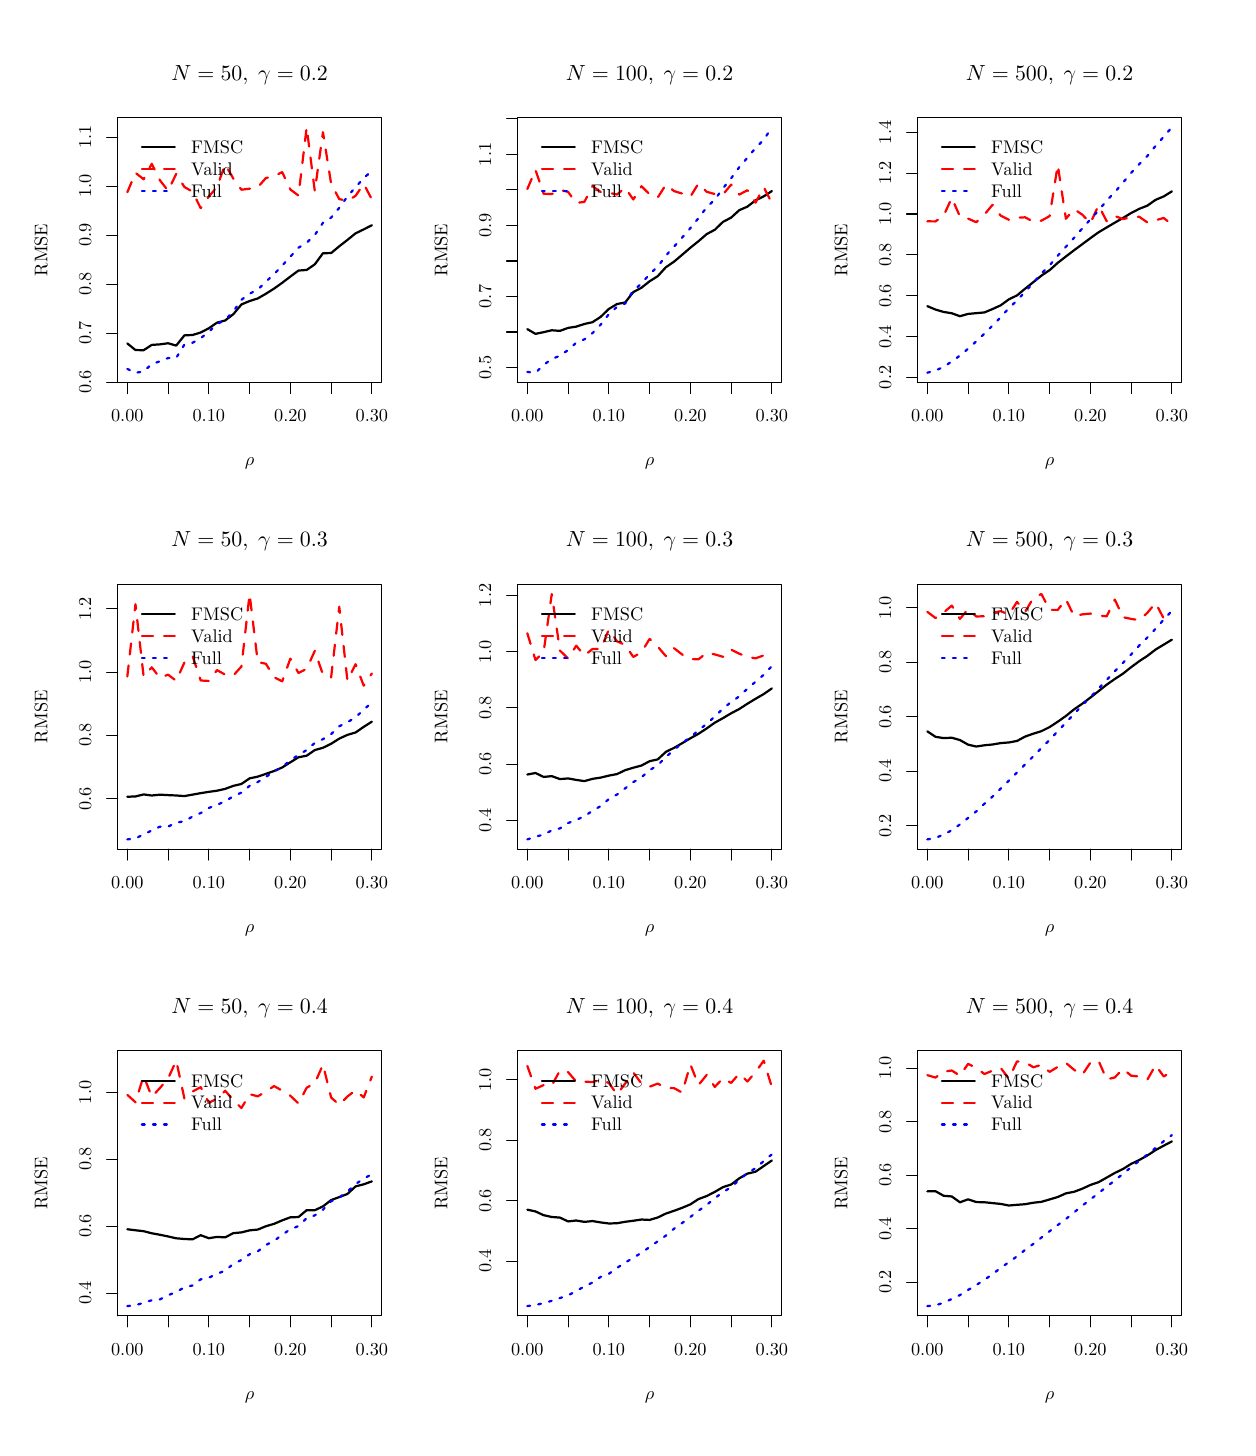
\begin{tikzpicture}[x=1pt,y=1pt]
\definecolor{fillColor}{RGB}{255,255,255}
\path[use as bounding box,fill=fillColor,fill opacity=0.00] (0,0) rectangle (433.62,505.89);
\begin{scope}
\path[clip] ( 32.47,377.65) rectangle (127.91,473.42);
\definecolor{drawColor}{RGB}{0,0,0}

\path[draw=drawColor,line width= 0.8pt,line join=round,line cap=round] ( 36.01,391.78) --
	( 38.95,389.39) --
	( 41.90,389.33) --
	( 44.84,391.25) --
	( 47.79,391.45) --
	( 50.73,391.85) --
	( 53.68,391.00) --
	( 56.63,394.70) --
	( 59.57,394.83) --
	( 62.52,395.73) --
	( 65.46,397.26) --
	( 68.41,399.29) --
	( 71.35,400.08) --
	( 74.30,402.33) --
	( 77.24,405.87) --
	( 80.19,407.10) --
	( 83.14,408.04) --
	( 86.08,409.73) --
	( 89.03,411.60) --
	( 91.97,413.69) --
	( 94.92,415.95) --
	( 97.86,418.12) --
	(100.81,418.34) --
	(103.75,420.36) --
	(106.70,424.37) --
	(109.65,424.44) --
	(112.59,426.89) --
	(115.54,429.18) --
	(118.48,431.57) --
	(121.43,432.99) --
	(124.37,434.49);
\end{scope}
\begin{scope}
\path[clip] (  0.00,  0.00) rectangle (433.62,505.89);
\definecolor{drawColor}{RGB}{0,0,0}

\path[draw=drawColor,line width= 0.4pt,line join=round,line cap=round] ( 36.01,377.65) -- (124.37,377.65);

\path[draw=drawColor,line width= 0.4pt,line join=round,line cap=round] ( 36.01,377.65) -- ( 36.01,373.69);

\path[draw=drawColor,line width= 0.4pt,line join=round,line cap=round] ( 50.73,377.65) -- ( 50.73,373.69);

\path[draw=drawColor,line width= 0.4pt,line join=round,line cap=round] ( 65.46,377.65) -- ( 65.46,373.69);

\path[draw=drawColor,line width= 0.4pt,line join=round,line cap=round] ( 80.19,377.65) -- ( 80.19,373.69);

\path[draw=drawColor,line width= 0.4pt,line join=round,line cap=round] ( 94.92,377.65) -- ( 94.92,373.69);

\path[draw=drawColor,line width= 0.4pt,line join=round,line cap=round] (109.65,377.65) -- (109.65,373.69);

\path[draw=drawColor,line width= 0.4pt,line join=round,line cap=round] (124.37,377.65) -- (124.37,373.69);

\node[text=drawColor,anchor=base,inner sep=0pt, outer sep=0pt, scale=  0.66] at ( 36.01,363.40) {0.00};

\node[text=drawColor,anchor=base,inner sep=0pt, outer sep=0pt, scale=  0.66] at ( 65.46,363.40) {0.10};

\node[text=drawColor,anchor=base,inner sep=0pt, outer sep=0pt, scale=  0.66] at ( 94.92,363.40) {0.20};

\node[text=drawColor,anchor=base,inner sep=0pt, outer sep=0pt, scale=  0.66] at (124.37,363.40) {0.30};

\path[draw=drawColor,line width= 0.4pt,line join=round,line cap=round] ( 32.47,377.78) -- ( 32.47,466.35);

\path[draw=drawColor,line width= 0.4pt,line join=round,line cap=round] ( 32.47,377.78) -- ( 28.51,377.78);

\path[draw=drawColor,line width= 0.4pt,line join=round,line cap=round] ( 32.47,395.49) -- ( 28.51,395.49);

\path[draw=drawColor,line width= 0.4pt,line join=round,line cap=round] ( 32.47,413.21) -- ( 28.51,413.21);

\path[draw=drawColor,line width= 0.4pt,line join=round,line cap=round] ( 32.47,430.92) -- ( 28.51,430.92);

\path[draw=drawColor,line width= 0.4pt,line join=round,line cap=round] ( 32.47,448.63) -- ( 28.51,448.63);

\path[draw=drawColor,line width= 0.4pt,line join=round,line cap=round] ( 32.47,466.35) -- ( 28.51,466.35);

\node[text=drawColor,rotate= 90.00,anchor=base,inner sep=0pt, outer sep=0pt, scale=  0.66] at ( 22.97,377.78) {0.6};

\node[text=drawColor,rotate= 90.00,anchor=base,inner sep=0pt, outer sep=0pt, scale=  0.66] at ( 22.97,395.49) {0.7};

\node[text=drawColor,rotate= 90.00,anchor=base,inner sep=0pt, outer sep=0pt, scale=  0.66] at ( 22.97,413.21) {0.8};

\node[text=drawColor,rotate= 90.00,anchor=base,inner sep=0pt, outer sep=0pt, scale=  0.66] at ( 22.97,430.92) {0.9};

\node[text=drawColor,rotate= 90.00,anchor=base,inner sep=0pt, outer sep=0pt, scale=  0.66] at ( 22.97,448.63) {1.0};

\node[text=drawColor,rotate= 90.00,anchor=base,inner sep=0pt, outer sep=0pt, scale=  0.66] at ( 22.97,466.35) {1.1};

\path[draw=drawColor,line width= 0.4pt,line join=round,line cap=round] ( 32.47,377.65) --
	(127.91,377.65) --
	(127.91,473.42) --
	( 32.47,473.42) --
	( 32.47,377.65);
\end{scope}
\begin{scope}
\path[clip] (  0.00,337.26) rectangle (144.54,505.89);
\definecolor{drawColor}{RGB}{0,0,0}

\node[text=drawColor,anchor=base,inner sep=0pt, outer sep=0pt, scale=  0.79] at ( 80.19,486.92) {\bfseries $N=50, \;\gamma=0.2$};

\node[text=drawColor,anchor=base,inner sep=0pt, outer sep=0pt, scale=  0.66] at ( 80.19,347.56) {$\rho$};

\node[text=drawColor,rotate= 90.00,anchor=base,inner sep=0pt, outer sep=0pt, scale=  0.66] at (  7.13,425.53) {RMSE};
\end{scope}
\begin{scope}
\path[clip] ( 32.47,377.65) rectangle (127.91,473.42);
\definecolor{drawColor}{RGB}{255,0,0}

\path[draw=drawColor,line width= 0.8pt,dash pattern=on 4pt off 4pt ,line join=round,line cap=round] ( 36.01,446.41) --
	( 38.95,453.44) --
	( 41.90,451.11) --
	( 44.84,456.70) --
	( 47.79,450.74) --
	( 50.73,446.94) --
	( 53.68,453.05) --
	( 56.63,448.32) --
	( 59.57,446.61) --
	( 62.52,440.66) --
	( 65.46,444.87) --
	( 68.41,448.31) --
	( 71.35,456.51) --
	( 74.30,451.38) --
	( 77.24,447.33) --
	( 80.19,447.71) --
	( 83.14,448.22) --
	( 86.08,451.55) --
	( 89.03,452.25) --
	( 91.97,453.68) --
	( 94.92,447.42) --
	( 97.86,445.20) --
	(100.81,469.87) --
	(103.75,446.86) --
	(106.70,468.12) --
	(109.65,449.48) --
	(112.59,443.95) --
	(115.54,443.29) --
	(118.48,445.13) --
	(121.43,449.41) --
	(124.37,443.86);
\definecolor{drawColor}{RGB}{0,0,255}

\path[draw=drawColor,line width= 0.8pt,dash pattern=on 1pt off 3pt ,line join=round,line cap=round] ( 36.01,382.57) --
	( 38.95,381.20) --
	( 41.90,381.63) --
	( 44.84,384.36) --
	( 47.79,385.33) --
	( 50.73,386.49) --
	( 53.68,386.56) --
	( 56.63,391.37) --
	( 59.57,392.03) --
	( 62.52,393.66) --
	( 65.46,396.02) --
	( 68.41,398.72) --
	( 71.35,400.32) --
	( 74.30,403.32) --
	( 77.24,407.55) --
	( 80.19,409.75) --
	( 83.14,411.23) --
	( 86.08,414.08) --
	( 89.03,416.81) --
	( 91.97,419.90) --
	( 94.92,423.13) --
	( 97.86,426.38) --
	(100.81,428.17) --
	(103.75,430.96) --
	(106.70,435.37) --
	(109.65,437.26) --
	(112.59,440.77) --
	(115.54,444.87) --
	(118.48,448.24) --
	(121.43,451.53) --
	(124.37,454.16);
\definecolor{drawColor}{RGB}{0,0,0}

\path[draw=drawColor,line width= 0.8pt,line join=round,line cap=round] ( 41.28,462.63) -- ( 53.16,462.63);
\definecolor{drawColor}{RGB}{255,0,0}

\path[draw=drawColor,line width= 0.8pt,dash pattern=on 4pt off 4pt ,line join=round,line cap=round] ( 41.28,454.71) -- ( 53.16,454.71);
\definecolor{drawColor}{RGB}{0,0,255}

\path[draw=drawColor,line width= 0.8pt,dash pattern=on 1pt off 3pt ,line join=round,line cap=round] ( 41.28,446.79) -- ( 53.16,446.79);
\definecolor{drawColor}{RGB}{0,0,0}

\node[text=drawColor,anchor=base west,inner sep=0pt, outer sep=0pt, scale=  0.66] at ( 59.10,460.35) {FMSC};

\node[text=drawColor,anchor=base west,inner sep=0pt, outer sep=0pt, scale=  0.66] at ( 59.10,452.43) {Valid};

\node[text=drawColor,anchor=base west,inner sep=0pt, outer sep=0pt, scale=  0.66] at ( 59.10,444.51) {Full};
\end{scope}
\begin{scope}
\path[clip] (177.01,377.65) rectangle (272.45,473.42);
\definecolor{drawColor}{RGB}{0,0,0}

\path[draw=drawColor,line width= 0.8pt,line join=round,line cap=round] (180.55,396.95) --
	(183.49,395.25) --
	(186.44,395.86) --
	(189.38,396.54) --
	(192.33,396.32) --
	(195.27,397.40) --
	(198.22,397.85) --
	(201.17,398.82) --
	(204.11,399.46) --
	(207.06,401.40) --
	(210.00,404.24) --
	(212.95,406.02) --
	(215.89,406.58) --
	(218.84,410.34) --
	(221.78,411.91) --
	(224.73,414.24) --
	(227.68,416.10) --
	(230.62,419.33) --
	(233.57,421.34) --
	(236.51,423.83) --
	(239.46,426.37) --
	(242.40,428.72) --
	(245.35,431.28) --
	(248.29,432.86) --
	(251.24,435.70) --
	(254.19,437.25) --
	(257.13,439.93) --
	(260.08,441.22) --
	(263.02,443.50) --
	(265.97,444.94) --
	(268.91,446.84);
\end{scope}
\begin{scope}
\path[clip] (  0.00,  0.00) rectangle (433.62,505.89);
\definecolor{drawColor}{RGB}{0,0,0}

\path[draw=drawColor,line width= 0.4pt,line join=round,line cap=round] (180.55,377.65) -- (268.91,377.65);

\path[draw=drawColor,line width= 0.4pt,line join=round,line cap=round] (180.55,377.65) -- (180.55,373.69);

\path[draw=drawColor,line width= 0.4pt,line join=round,line cap=round] (195.27,377.65) -- (195.27,373.69);

\path[draw=drawColor,line width= 0.4pt,line join=round,line cap=round] (210.00,377.65) -- (210.00,373.69);

\path[draw=drawColor,line width= 0.4pt,line join=round,line cap=round] (224.73,377.65) -- (224.73,373.69);

\path[draw=drawColor,line width= 0.4pt,line join=round,line cap=round] (239.46,377.65) -- (239.46,373.69);

\path[draw=drawColor,line width= 0.4pt,line join=round,line cap=round] (254.19,377.65) -- (254.19,373.69);

\path[draw=drawColor,line width= 0.4pt,line join=round,line cap=round] (268.91,377.65) -- (268.91,373.69);

\node[text=drawColor,anchor=base,inner sep=0pt, outer sep=0pt, scale=  0.66] at (180.55,363.40) {0.00};

\node[text=drawColor,anchor=base,inner sep=0pt, outer sep=0pt, scale=  0.66] at (210.00,363.40) {0.10};

\node[text=drawColor,anchor=base,inner sep=0pt, outer sep=0pt, scale=  0.66] at (239.46,363.40) {0.20};

\node[text=drawColor,anchor=base,inner sep=0pt, outer sep=0pt, scale=  0.66] at (268.91,363.40) {0.30};

\path[draw=drawColor,line width= 0.4pt,line join=round,line cap=round] (177.01,383.09) -- (177.01,472.91);

\path[draw=drawColor,line width= 0.4pt,line join=round,line cap=round] (177.01,383.09) -- (173.05,383.09);

\path[draw=drawColor,line width= 0.4pt,line join=round,line cap=round] (177.01,395.92) -- (173.05,395.92);

\path[draw=drawColor,line width= 0.4pt,line join=round,line cap=round] (177.01,408.75) -- (173.05,408.75);

\path[draw=drawColor,line width= 0.4pt,line join=round,line cap=round] (177.01,421.58) -- (173.05,421.58);

\path[draw=drawColor,line width= 0.4pt,line join=round,line cap=round] (177.01,434.41) -- (173.05,434.41);

\path[draw=drawColor,line width= 0.4pt,line join=round,line cap=round] (177.01,447.25) -- (173.05,447.25);

\path[draw=drawColor,line width= 0.4pt,line join=round,line cap=round] (177.01,460.08) -- (173.05,460.08);

\path[draw=drawColor,line width= 0.4pt,line join=round,line cap=round] (177.01,472.91) -- (173.05,472.91);

\node[text=drawColor,rotate= 90.00,anchor=base,inner sep=0pt, outer sep=0pt, scale=  0.66] at (167.51,383.09) {0.5};

\node[text=drawColor,rotate= 90.00,anchor=base,inner sep=0pt, outer sep=0pt, scale=  0.66] at (167.51,408.75) {0.7};

\node[text=drawColor,rotate= 90.00,anchor=base,inner sep=0pt, outer sep=0pt, scale=  0.66] at (167.51,434.41) {0.9};

\node[text=drawColor,rotate= 90.00,anchor=base,inner sep=0pt, outer sep=0pt, scale=  0.66] at (167.51,460.08) {1.1};

\path[draw=drawColor,line width= 0.4pt,line join=round,line cap=round] (177.01,377.65) --
	(272.45,377.65) --
	(272.45,473.42) --
	(177.01,473.42) --
	(177.01,377.65);
\end{scope}
\begin{scope}
\path[clip] (144.54,337.26) rectangle (289.08,505.89);
\definecolor{drawColor}{RGB}{0,0,0}

\node[text=drawColor,anchor=base,inner sep=0pt, outer sep=0pt, scale=  0.79] at (224.73,486.92) {\bfseries $N=100, \;\gamma=0.2$};

\node[text=drawColor,anchor=base,inner sep=0pt, outer sep=0pt, scale=  0.66] at (224.73,347.56) {$\rho$};

\node[text=drawColor,rotate= 90.00,anchor=base,inner sep=0pt, outer sep=0pt, scale=  0.66] at (151.67,425.53) {RMSE};
\end{scope}
\begin{scope}
\path[clip] (177.01,377.65) rectangle (272.45,473.42);
\definecolor{drawColor}{RGB}{255,0,0}

\path[draw=drawColor,line width= 0.8pt,dash pattern=on 4pt off 4pt ,line join=round,line cap=round] (180.55,447.58) --
	(183.49,454.50) --
	(186.44,445.85) --
	(189.38,445.77) --
	(192.33,447.24) --
	(195.27,446.54) --
	(198.22,442.53) --
	(201.17,442.94) --
	(204.11,448.64) --
	(207.06,446.50) --
	(210.00,446.26) --
	(212.95,445.59) --
	(215.89,448.02) --
	(218.84,443.80) --
	(221.78,448.58) --
	(224.73,445.70) --
	(227.68,444.52) --
	(230.62,449.17) --
	(233.57,446.84) --
	(236.51,445.93) --
	(239.46,444.82) --
	(242.40,449.59) --
	(245.35,446.58) --
	(248.29,445.77) --
	(251.24,445.64) --
	(254.19,449.15) --
	(257.13,445.57) --
	(260.08,447.15) --
	(263.02,442.66) --
	(265.97,448.24) --
	(268.91,442.55);
\definecolor{drawColor}{RGB}{0,0,255}

\path[draw=drawColor,line width= 0.8pt,dash pattern=on 1pt off 3pt ,line join=round,line cap=round] (180.55,381.48) --
	(183.49,381.20) --
	(186.44,384.00) --
	(189.38,386.18) --
	(192.33,387.32) --
	(195.27,389.40) --
	(198.22,392.02) --
	(201.17,393.27) --
	(204.11,395.53) --
	(207.06,398.58) --
	(210.00,402.33) --
	(212.95,405.02) --
	(215.89,406.20) --
	(218.84,410.91) --
	(221.78,413.39) --
	(224.73,416.86) --
	(227.68,419.51) --
	(230.62,423.53) --
	(233.57,426.77) --
	(236.51,430.06) --
	(239.46,433.46) --
	(242.40,437.07) --
	(245.35,440.94) --
	(248.29,443.76) --
	(251.24,447.83) --
	(254.19,451.46) --
	(257.13,455.46) --
	(260.08,458.90) --
	(263.02,462.40) --
	(265.97,465.37) --
	(268.91,469.87);
\definecolor{drawColor}{RGB}{0,0,0}

\path[draw=drawColor,line width= 0.8pt,line join=round,line cap=round] (185.82,462.63) -- (197.70,462.63);
\definecolor{drawColor}{RGB}{255,0,0}

\path[draw=drawColor,line width= 0.8pt,dash pattern=on 4pt off 4pt ,line join=round,line cap=round] (185.82,454.71) -- (197.70,454.71);
\definecolor{drawColor}{RGB}{0,0,255}

\path[draw=drawColor,line width= 0.8pt,dash pattern=on 1pt off 3pt ,line join=round,line cap=round] (185.82,446.79) -- (197.70,446.79);
\definecolor{drawColor}{RGB}{0,0,0}

\node[text=drawColor,anchor=base west,inner sep=0pt, outer sep=0pt, scale=  0.66] at (203.64,460.35) {FMSC};

\node[text=drawColor,anchor=base west,inner sep=0pt, outer sep=0pt, scale=  0.66] at (203.64,452.43) {Valid};

\node[text=drawColor,anchor=base west,inner sep=0pt, outer sep=0pt, scale=  0.66] at (203.64,444.51) {Full};
\end{scope}
\begin{scope}
\path[clip] (321.55,377.65) rectangle (416.99,473.42);
\definecolor{drawColor}{RGB}{0,0,0}

\path[draw=drawColor,line width= 0.8pt,line join=round,line cap=round] (325.09,405.26) --
	(328.03,404.03) --
	(330.98,403.16) --
	(333.92,402.69) --
	(336.87,401.62) --
	(339.81,402.45) --
	(342.76,402.72) --
	(345.71,402.99) --
	(348.65,404.21) --
	(351.60,405.56) --
	(354.54,407.71) --
	(357.49,409.14) --
	(360.43,411.57) --
	(363.38,413.92) --
	(366.32,416.30) --
	(369.27,418.26) --
	(372.22,420.91) --
	(375.16,423.20) --
	(378.11,425.46) --
	(381.05,427.62) --
	(384.00,429.82) --
	(386.94,431.93) --
	(389.89,433.69) --
	(392.83,435.42) --
	(395.78,437.12) --
	(398.73,438.91) --
	(401.67,440.42) --
	(404.62,441.59) --
	(407.56,443.67) --
	(410.51,444.91) --
	(413.45,446.73);
\end{scope}
\begin{scope}
\path[clip] (  0.00,  0.00) rectangle (433.62,505.89);
\definecolor{drawColor}{RGB}{0,0,0}

\path[draw=drawColor,line width= 0.4pt,line join=round,line cap=round] (325.09,377.65) -- (413.45,377.65);

\path[draw=drawColor,line width= 0.4pt,line join=round,line cap=round] (325.09,377.65) -- (325.09,373.69);

\path[draw=drawColor,line width= 0.4pt,line join=round,line cap=round] (339.81,377.65) -- (339.81,373.69);

\path[draw=drawColor,line width= 0.4pt,line join=round,line cap=round] (354.54,377.65) -- (354.54,373.69);

\path[draw=drawColor,line width= 0.4pt,line join=round,line cap=round] (369.27,377.65) -- (369.27,373.69);

\path[draw=drawColor,line width= 0.4pt,line join=round,line cap=round] (384.00,377.65) -- (384.00,373.69);

\path[draw=drawColor,line width= 0.4pt,line join=round,line cap=round] (398.73,377.65) -- (398.73,373.69);

\path[draw=drawColor,line width= 0.4pt,line join=round,line cap=round] (413.45,377.65) -- (413.45,373.69);

\node[text=drawColor,anchor=base,inner sep=0pt, outer sep=0pt, scale=  0.66] at (325.09,363.40) {0.00};

\node[text=drawColor,anchor=base,inner sep=0pt, outer sep=0pt, scale=  0.66] at (354.54,363.40) {0.10};

\node[text=drawColor,anchor=base,inner sep=0pt, outer sep=0pt, scale=  0.66] at (384.00,363.40) {0.20};

\node[text=drawColor,anchor=base,inner sep=0pt, outer sep=0pt, scale=  0.66] at (413.45,363.40) {0.30};

\path[draw=drawColor,line width= 0.4pt,line join=round,line cap=round] (321.55,379.53) -- (321.55,468.04);

\path[draw=drawColor,line width= 0.4pt,line join=round,line cap=round] (321.55,379.53) -- (317.59,379.53);

\path[draw=drawColor,line width= 0.4pt,line join=round,line cap=round] (321.55,394.28) -- (317.59,394.28);

\path[draw=drawColor,line width= 0.4pt,line join=round,line cap=round] (321.55,409.03) -- (317.59,409.03);

\path[draw=drawColor,line width= 0.4pt,line join=round,line cap=round] (321.55,423.79) -- (317.59,423.79);

\path[draw=drawColor,line width= 0.4pt,line join=round,line cap=round] (321.55,438.54) -- (317.59,438.54);

\path[draw=drawColor,line width= 0.4pt,line join=round,line cap=round] (321.55,453.29) -- (317.59,453.29);

\path[draw=drawColor,line width= 0.4pt,line join=round,line cap=round] (321.55,468.04) -- (317.59,468.04);

\node[text=drawColor,rotate= 90.00,anchor=base,inner sep=0pt, outer sep=0pt, scale=  0.66] at (312.05,379.53) {0.2};

\node[text=drawColor,rotate= 90.00,anchor=base,inner sep=0pt, outer sep=0pt, scale=  0.66] at (312.05,394.28) {0.4};

\node[text=drawColor,rotate= 90.00,anchor=base,inner sep=0pt, outer sep=0pt, scale=  0.66] at (312.05,409.03) {0.6};

\node[text=drawColor,rotate= 90.00,anchor=base,inner sep=0pt, outer sep=0pt, scale=  0.66] at (312.05,423.79) {0.8};

\node[text=drawColor,rotate= 90.00,anchor=base,inner sep=0pt, outer sep=0pt, scale=  0.66] at (312.05,438.54) {1.0};

\node[text=drawColor,rotate= 90.00,anchor=base,inner sep=0pt, outer sep=0pt, scale=  0.66] at (312.05,453.29) {1.2};

\node[text=drawColor,rotate= 90.00,anchor=base,inner sep=0pt, outer sep=0pt, scale=  0.66] at (312.05,468.04) {1.4};

\path[draw=drawColor,line width= 0.4pt,line join=round,line cap=round] (321.55,377.65) --
	(416.99,377.65) --
	(416.99,473.42) --
	(321.55,473.42) --
	(321.55,377.65);
\end{scope}
\begin{scope}
\path[clip] (289.08,337.26) rectangle (433.62,505.89);
\definecolor{drawColor}{RGB}{0,0,0}

\node[text=drawColor,anchor=base,inner sep=0pt, outer sep=0pt, scale=  0.79] at (369.27,486.92) {\bfseries $N=500, \;\gamma=0.2$};

\node[text=drawColor,anchor=base,inner sep=0pt, outer sep=0pt, scale=  0.66] at (369.27,347.56) {$\rho$};

\node[text=drawColor,rotate= 90.00,anchor=base,inner sep=0pt, outer sep=0pt, scale=  0.66] at (296.21,425.53) {RMSE};
\end{scope}
\begin{scope}
\path[clip] (321.55,377.65) rectangle (416.99,473.42);
\definecolor{drawColor}{RGB}{255,0,0}

\path[draw=drawColor,line width= 0.8pt,dash pattern=on 4pt off 4pt ,line join=round,line cap=round] (325.09,435.91) --
	(328.03,435.88) --
	(330.98,437.97) --
	(333.92,444.35) --
	(336.87,437.65) --
	(339.81,436.89) --
	(342.76,435.59) --
	(345.71,438.36) --
	(348.65,441.87) --
	(351.60,437.95) --
	(354.54,436.47) --
	(357.49,437.19) --
	(360.43,437.36) --
	(363.38,435.76) --
	(366.32,436.15) --
	(369.27,437.80) --
	(372.22,456.27) --
	(375.16,436.83) --
	(378.11,440.32) --
	(381.05,438.35) --
	(384.00,435.25) --
	(386.94,441.66) --
	(389.89,435.98) --
	(392.83,437.87) --
	(395.78,436.69) --
	(398.73,437.44) --
	(401.67,437.54) --
	(404.62,435.49) --
	(407.56,436.28) --
	(410.51,437.12) --
	(413.45,434.72);
\definecolor{drawColor}{RGB}{0,0,255}

\path[draw=drawColor,line width= 0.8pt,dash pattern=on 1pt off 3pt ,line join=round,line cap=round] (325.09,381.20) --
	(328.03,382.01) --
	(330.98,383.30) --
	(333.92,385.29) --
	(336.87,387.38) --
	(339.81,389.86) --
	(342.76,392.53) --
	(345.71,395.32) --
	(348.65,398.25) --
	(351.60,401.26) --
	(354.54,404.51) --
	(357.49,407.31) --
	(360.43,410.44) --
	(363.38,413.68) --
	(366.32,417.11) --
	(369.27,419.98) --
	(372.22,423.49) --
	(375.16,426.73) --
	(378.11,429.95) --
	(381.05,433.30) --
	(384.00,436.61) --
	(386.94,439.80) --
	(389.89,443.39) --
	(392.83,446.43) --
	(395.78,449.88) --
	(398.73,453.41) --
	(401.67,456.58) --
	(404.62,459.55) --
	(407.56,463.14) --
	(410.51,466.48) --
	(413.45,469.87);
\definecolor{drawColor}{RGB}{0,0,0}

\path[draw=drawColor,line width= 0.8pt,line join=round,line cap=round] (330.36,462.63) -- (342.24,462.63);
\definecolor{drawColor}{RGB}{255,0,0}

\path[draw=drawColor,line width= 0.8pt,dash pattern=on 4pt off 4pt ,line join=round,line cap=round] (330.36,454.71) -- (342.24,454.71);
\definecolor{drawColor}{RGB}{0,0,255}

\path[draw=drawColor,line width= 0.8pt,dash pattern=on 1pt off 3pt ,line join=round,line cap=round] (330.36,446.79) -- (342.24,446.79);
\definecolor{drawColor}{RGB}{0,0,0}

\node[text=drawColor,anchor=base west,inner sep=0pt, outer sep=0pt, scale=  0.66] at (348.18,460.35) {FMSC};

\node[text=drawColor,anchor=base west,inner sep=0pt, outer sep=0pt, scale=  0.66] at (348.18,452.43) {Valid};

\node[text=drawColor,anchor=base west,inner sep=0pt, outer sep=0pt, scale=  0.66] at (348.18,444.51) {Full};
\end{scope}
\begin{scope}
\path[clip] ( 32.47,209.02) rectangle (127.91,304.79);
\definecolor{drawColor}{RGB}{0,0,0}

\path[draw=drawColor,line width= 0.8pt,line join=round,line cap=round] ( 36.01,227.98) --
	( 38.95,228.09) --
	( 41.90,228.82) --
	( 44.84,228.43) --
	( 47.79,228.73) --
	( 50.73,228.57) --
	( 53.68,228.44) --
	( 56.63,228.22) --
	( 59.57,228.75) --
	( 62.52,229.28) --
	( 65.46,229.75) --
	( 68.41,230.16) --
	( 71.35,230.82) --
	( 74.30,231.91) --
	( 77.24,232.60) --
	( 80.19,234.63) --
	( 83.14,235.24) --
	( 86.08,236.25) --
	( 89.03,237.29) --
	( 91.97,238.56) --
	( 94.92,240.43) --
	( 97.86,242.25) --
	(100.81,242.81) --
	(103.75,244.85) --
	(106.70,245.68) --
	(109.65,247.12) --
	(112.59,248.99) --
	(115.54,250.34) --
	(118.48,251.20) --
	(121.43,253.23) --
	(124.37,255.11);
\end{scope}
\begin{scope}
\path[clip] (  0.00,  0.00) rectangle (433.62,505.89);
\definecolor{drawColor}{RGB}{0,0,0}

\path[draw=drawColor,line width= 0.4pt,line join=round,line cap=round] ( 36.01,209.02) -- (124.37,209.02);

\path[draw=drawColor,line width= 0.4pt,line join=round,line cap=round] ( 36.01,209.02) -- ( 36.01,205.06);

\path[draw=drawColor,line width= 0.4pt,line join=round,line cap=round] ( 50.73,209.02) -- ( 50.73,205.06);

\path[draw=drawColor,line width= 0.4pt,line join=round,line cap=round] ( 65.46,209.02) -- ( 65.46,205.06);

\path[draw=drawColor,line width= 0.4pt,line join=round,line cap=round] ( 80.19,209.02) -- ( 80.19,205.06);

\path[draw=drawColor,line width= 0.4pt,line join=round,line cap=round] ( 94.92,209.02) -- ( 94.92,205.06);

\path[draw=drawColor,line width= 0.4pt,line join=round,line cap=round] (109.65,209.02) -- (109.65,205.06);

\path[draw=drawColor,line width= 0.4pt,line join=round,line cap=round] (124.37,209.02) -- (124.37,205.06);

\node[text=drawColor,anchor=base,inner sep=0pt, outer sep=0pt, scale=  0.66] at ( 36.01,194.77) {0.00};

\node[text=drawColor,anchor=base,inner sep=0pt, outer sep=0pt, scale=  0.66] at ( 65.46,194.77) {0.10};

\node[text=drawColor,anchor=base,inner sep=0pt, outer sep=0pt, scale=  0.66] at ( 94.92,194.77) {0.20};

\node[text=drawColor,anchor=base,inner sep=0pt, outer sep=0pt, scale=  0.66] at (124.37,194.77) {0.30};

\path[draw=drawColor,line width= 0.4pt,line join=round,line cap=round] ( 32.47,227.33) -- ( 32.47,295.88);

\path[draw=drawColor,line width= 0.4pt,line join=round,line cap=round] ( 32.47,227.33) -- ( 28.51,227.33);

\path[draw=drawColor,line width= 0.4pt,line join=round,line cap=round] ( 32.47,250.18) -- ( 28.51,250.18);

\path[draw=drawColor,line width= 0.4pt,line join=round,line cap=round] ( 32.47,273.03) -- ( 28.51,273.03);

\path[draw=drawColor,line width= 0.4pt,line join=round,line cap=round] ( 32.47,295.88) -- ( 28.51,295.88);

\node[text=drawColor,rotate= 90.00,anchor=base,inner sep=0pt, outer sep=0pt, scale=  0.66] at ( 22.97,227.33) {0.6};

\node[text=drawColor,rotate= 90.00,anchor=base,inner sep=0pt, outer sep=0pt, scale=  0.66] at ( 22.97,250.18) {0.8};

\node[text=drawColor,rotate= 90.00,anchor=base,inner sep=0pt, outer sep=0pt, scale=  0.66] at ( 22.97,273.03) {1.0};

\node[text=drawColor,rotate= 90.00,anchor=base,inner sep=0pt, outer sep=0pt, scale=  0.66] at ( 22.97,295.88) {1.2};

\path[draw=drawColor,line width= 0.4pt,line join=round,line cap=round] ( 32.47,209.02) --
	(127.91,209.02) --
	(127.91,304.79) --
	( 32.47,304.79) --
	( 32.47,209.02);
\end{scope}
\begin{scope}
\path[clip] (  0.00,168.63) rectangle (144.54,337.26);
\definecolor{drawColor}{RGB}{0,0,0}

\node[text=drawColor,anchor=base,inner sep=0pt, outer sep=0pt, scale=  0.79] at ( 80.19,318.29) {\bfseries $N=50, \;\gamma=0.3$};

\node[text=drawColor,anchor=base,inner sep=0pt, outer sep=0pt, scale=  0.66] at ( 80.19,178.93) {$\rho$};

\node[text=drawColor,rotate= 90.00,anchor=base,inner sep=0pt, outer sep=0pt, scale=  0.66] at (  7.13,256.90) {RMSE};
\end{scope}
\begin{scope}
\path[clip] ( 32.47,209.02) rectangle (127.91,304.79);
\definecolor{drawColor}{RGB}{255,0,0}

\path[draw=drawColor,line width= 0.8pt,dash pattern=on 4pt off 4pt ,line join=round,line cap=round] ( 36.01,271.45) --
	( 38.95,297.56) --
	( 41.90,271.41) --
	( 44.84,274.75) --
	( 47.79,270.92) --
	( 50.73,272.10) --
	( 53.68,269.85) --
	( 56.63,276.50) --
	( 59.57,278.83) --
	( 62.52,269.99) --
	( 65.46,269.82) --
	( 68.41,273.75) --
	( 71.35,272.10) --
	( 74.30,271.79) --
	( 77.24,275.04) --
	( 80.19,301.24) --
	( 83.14,276.65) --
	( 86.08,276.03) --
	( 89.03,271.17) --
	( 91.97,269.68) --
	( 94.92,277.90) --
	( 97.86,272.69) --
	(100.81,274.21) --
	(103.75,280.69) --
	(106.70,272.10) --
	(109.65,271.13) --
	(112.59,296.61) --
	(115.54,269.95) --
	(118.48,275.89) --
	(121.43,268.12) --
	(124.37,272.52);
\definecolor{drawColor}{RGB}{0,0,255}

\path[draw=drawColor,line width= 0.8pt,dash pattern=on 1pt off 3pt ,line join=round,line cap=round] ( 36.01,212.57) --
	( 38.95,212.94) --
	( 41.90,214.39) --
	( 44.84,215.80) --
	( 47.79,217.17) --
	( 50.73,217.18) --
	( 53.68,218.62) --
	( 56.63,219.14) --
	( 59.57,220.82) --
	( 62.52,222.09) --
	( 65.46,223.93) --
	( 68.41,225.06) --
	( 71.35,226.34) --
	( 74.30,228.15) --
	( 77.24,229.48) --
	( 80.19,231.92) --
	( 83.14,233.30) --
	( 86.08,235.16) --
	( 89.03,237.04) --
	( 91.97,238.79) --
	( 94.92,241.11) --
	( 97.86,243.13) --
	(100.81,244.84) --
	(103.75,247.43) --
	(106.70,248.79) --
	(109.65,250.61) --
	(112.59,253.44) --
	(115.54,254.91) --
	(118.48,256.69) --
	(121.43,259.46) --
	(124.37,262.02);
\definecolor{drawColor}{RGB}{0,0,0}

\path[draw=drawColor,line width= 0.8pt,line join=round,line cap=round] ( 41.28,294.00) -- ( 53.16,294.00);
\definecolor{drawColor}{RGB}{255,0,0}

\path[draw=drawColor,line width= 0.8pt,dash pattern=on 4pt off 4pt ,line join=round,line cap=round] ( 41.28,286.08) -- ( 53.16,286.08);
\definecolor{drawColor}{RGB}{0,0,255}

\path[draw=drawColor,line width= 0.8pt,dash pattern=on 1pt off 3pt ,line join=round,line cap=round] ( 41.28,278.16) -- ( 53.16,278.16);
\definecolor{drawColor}{RGB}{0,0,0}

\node[text=drawColor,anchor=base west,inner sep=0pt, outer sep=0pt, scale=  0.66] at ( 59.10,291.72) {FMSC};

\node[text=drawColor,anchor=base west,inner sep=0pt, outer sep=0pt, scale=  0.66] at ( 59.10,283.80) {Valid};

\node[text=drawColor,anchor=base west,inner sep=0pt, outer sep=0pt, scale=  0.66] at ( 59.10,275.88) {Full};
\end{scope}
\begin{scope}
\path[clip] (177.01,209.02) rectangle (272.45,304.79);
\definecolor{drawColor}{RGB}{0,0,0}

\path[draw=drawColor,line width= 0.8pt,line join=round,line cap=round] (180.55,236.01) --
	(183.49,236.56) --
	(186.44,235.14) --
	(189.38,235.43) --
	(192.33,234.36) --
	(195.27,234.60) --
	(198.22,234.07) --
	(201.17,233.63) --
	(204.11,234.45) --
	(207.06,234.90) --
	(210.00,235.62) --
	(212.95,236.17) --
	(215.89,237.58) --
	(218.84,238.47) --
	(221.78,239.25) --
	(224.73,240.83) --
	(227.68,241.48) --
	(230.62,244.20) --
	(233.57,245.65) --
	(236.51,247.33) --
	(239.46,249.10) --
	(242.40,250.73) --
	(245.35,252.67) --
	(248.29,254.74) --
	(251.24,256.39) --
	(254.19,258.14) --
	(257.13,259.68) --
	(260.08,261.60) --
	(263.02,263.38) --
	(265.97,265.08) --
	(268.91,267.13);
\end{scope}
\begin{scope}
\path[clip] (  0.00,  0.00) rectangle (433.62,505.89);
\definecolor{drawColor}{RGB}{0,0,0}

\path[draw=drawColor,line width= 0.4pt,line join=round,line cap=round] (180.55,209.02) -- (268.91,209.02);

\path[draw=drawColor,line width= 0.4pt,line join=round,line cap=round] (180.55,209.02) -- (180.55,205.06);

\path[draw=drawColor,line width= 0.4pt,line join=round,line cap=round] (195.27,209.02) -- (195.27,205.06);

\path[draw=drawColor,line width= 0.4pt,line join=round,line cap=round] (210.00,209.02) -- (210.00,205.06);

\path[draw=drawColor,line width= 0.4pt,line join=round,line cap=round] (224.73,209.02) -- (224.73,205.06);

\path[draw=drawColor,line width= 0.4pt,line join=round,line cap=round] (239.46,209.02) -- (239.46,205.06);

\path[draw=drawColor,line width= 0.4pt,line join=round,line cap=round] (254.19,209.02) -- (254.19,205.06);

\path[draw=drawColor,line width= 0.4pt,line join=round,line cap=round] (268.91,209.02) -- (268.91,205.06);

\node[text=drawColor,anchor=base,inner sep=0pt, outer sep=0pt, scale=  0.66] at (180.55,194.77) {0.00};

\node[text=drawColor,anchor=base,inner sep=0pt, outer sep=0pt, scale=  0.66] at (210.00,194.77) {0.10};

\node[text=drawColor,anchor=base,inner sep=0pt, outer sep=0pt, scale=  0.66] at (239.46,194.77) {0.20};

\node[text=drawColor,anchor=base,inner sep=0pt, outer sep=0pt, scale=  0.66] at (268.91,194.77) {0.30};

\path[draw=drawColor,line width= 0.4pt,line join=round,line cap=round] (177.01,219.45) -- (177.01,300.73);

\path[draw=drawColor,line width= 0.4pt,line join=round,line cap=round] (177.01,219.45) -- (173.05,219.45);

\path[draw=drawColor,line width= 0.4pt,line join=round,line cap=round] (177.01,239.77) -- (173.05,239.77);

\path[draw=drawColor,line width= 0.4pt,line join=round,line cap=round] (177.01,260.09) -- (173.05,260.09);

\path[draw=drawColor,line width= 0.4pt,line join=round,line cap=round] (177.01,280.41) -- (173.05,280.41);

\path[draw=drawColor,line width= 0.4pt,line join=round,line cap=round] (177.01,300.73) -- (173.05,300.73);

\node[text=drawColor,rotate= 90.00,anchor=base,inner sep=0pt, outer sep=0pt, scale=  0.66] at (167.51,219.45) {0.4};

\node[text=drawColor,rotate= 90.00,anchor=base,inner sep=0pt, outer sep=0pt, scale=  0.66] at (167.51,239.77) {0.6};

\node[text=drawColor,rotate= 90.00,anchor=base,inner sep=0pt, outer sep=0pt, scale=  0.66] at (167.51,260.09) {0.8};

\node[text=drawColor,rotate= 90.00,anchor=base,inner sep=0pt, outer sep=0pt, scale=  0.66] at (167.51,280.41) {1.0};

\node[text=drawColor,rotate= 90.00,anchor=base,inner sep=0pt, outer sep=0pt, scale=  0.66] at (167.51,300.73) {1.2};

\path[draw=drawColor,line width= 0.4pt,line join=round,line cap=round] (177.01,209.02) --
	(272.45,209.02) --
	(272.45,304.79) --
	(177.01,304.79) --
	(177.01,209.02);
\end{scope}
\begin{scope}
\path[clip] (144.54,168.63) rectangle (289.08,337.26);
\definecolor{drawColor}{RGB}{0,0,0}

\node[text=drawColor,anchor=base,inner sep=0pt, outer sep=0pt, scale=  0.79] at (224.73,318.29) {\bfseries $N=100, \;\gamma=0.3$};

\node[text=drawColor,anchor=base,inner sep=0pt, outer sep=0pt, scale=  0.66] at (224.73,178.93) {$\rho$};

\node[text=drawColor,rotate= 90.00,anchor=base,inner sep=0pt, outer sep=0pt, scale=  0.66] at (151.67,256.90) {RMSE};
\end{scope}
\begin{scope}
\path[clip] (177.01,209.02) rectangle (272.45,304.79);
\definecolor{drawColor}{RGB}{255,0,0}

\path[draw=drawColor,line width= 0.8pt,dash pattern=on 4pt off 4pt ,line join=round,line cap=round] (180.55,287.05) --
	(183.49,277.38) --
	(186.44,280.32) --
	(189.38,301.24) --
	(192.33,280.82) --
	(195.27,277.91) --
	(198.22,282.57) --
	(201.17,278.98) --
	(204.11,281.41) --
	(207.06,281.36) --
	(210.00,288.35) --
	(212.95,284.15) --
	(215.89,282.86) --
	(218.84,278.50) --
	(221.78,280.17) --
	(224.73,285.01) --
	(227.68,282.21) --
	(230.62,278.79) --
	(233.57,281.66) --
	(236.51,279.36) --
	(239.46,277.75) --
	(242.40,277.65) --
	(245.35,279.96) --
	(248.29,279.42) --
	(251.24,278.55) --
	(254.19,281.13) --
	(257.13,279.68) --
	(260.08,278.52) --
	(263.02,277.99) --
	(265.97,279.06) --
	(268.91,279.30);
\definecolor{drawColor}{RGB}{0,0,255}

\path[draw=drawColor,line width= 0.8pt,dash pattern=on 1pt off 3pt ,line join=round,line cap=round] (180.55,212.57) --
	(183.49,213.56) --
	(186.44,214.29) --
	(189.38,215.82) --
	(192.33,216.54) --
	(195.27,218.47) --
	(198.22,219.62) --
	(201.17,220.91) --
	(204.11,222.93) --
	(207.06,224.61) --
	(210.00,227.14) --
	(212.95,228.78) --
	(215.89,231.01) --
	(218.84,233.27) --
	(221.78,234.99) --
	(224.73,237.55) --
	(227.68,239.41) --
	(230.62,242.38) --
	(233.57,244.88) --
	(236.51,247.46) --
	(239.46,249.44) --
	(242.40,251.99) --
	(245.35,254.32) --
	(248.29,256.97) --
	(251.24,259.82) --
	(254.19,262.20) --
	(257.13,264.26) --
	(260.08,267.04) --
	(263.02,269.54) --
	(265.97,272.06) --
	(268.91,275.17);
\definecolor{drawColor}{RGB}{0,0,0}

\path[draw=drawColor,line width= 0.8pt,line join=round,line cap=round] (185.82,294.00) -- (197.70,294.00);
\definecolor{drawColor}{RGB}{255,0,0}

\path[draw=drawColor,line width= 0.8pt,dash pattern=on 4pt off 4pt ,line join=round,line cap=round] (185.82,286.08) -- (197.70,286.08);
\definecolor{drawColor}{RGB}{0,0,255}

\path[draw=drawColor,line width= 0.8pt,dash pattern=on 1pt off 3pt ,line join=round,line cap=round] (185.82,278.16) -- (197.70,278.16);
\definecolor{drawColor}{RGB}{0,0,0}

\node[text=drawColor,anchor=base west,inner sep=0pt, outer sep=0pt, scale=  0.66] at (203.64,291.72) {FMSC};

\node[text=drawColor,anchor=base west,inner sep=0pt, outer sep=0pt, scale=  0.66] at (203.64,283.80) {Valid};

\node[text=drawColor,anchor=base west,inner sep=0pt, outer sep=0pt, scale=  0.66] at (203.64,275.88) {Full};
\end{scope}
\begin{scope}
\path[clip] (321.55,209.02) rectangle (416.99,304.79);
\definecolor{drawColor}{RGB}{0,0,0}

\path[draw=drawColor,line width= 0.8pt,line join=round,line cap=round] (325.09,251.61) --
	(328.03,249.64) --
	(330.98,249.17) --
	(333.92,249.31) --
	(336.87,248.47) --
	(339.81,246.81) --
	(342.76,246.13) --
	(345.71,246.58) --
	(348.65,246.86) --
	(351.60,247.37) --
	(354.54,247.60) --
	(357.49,248.14) --
	(360.43,249.73) --
	(363.38,250.77) --
	(366.32,251.68) --
	(369.27,253.16) --
	(372.22,255.09) --
	(375.16,257.17) --
	(378.11,259.55) --
	(381.05,261.58) --
	(384.00,263.81) --
	(386.94,266.12) --
	(389.89,268.47) --
	(392.83,270.53) --
	(395.78,272.45) --
	(398.73,274.80) --
	(401.67,276.97) --
	(404.62,278.90) --
	(407.56,281.17) --
	(410.51,282.95) --
	(413.45,284.73);
\end{scope}
\begin{scope}
\path[clip] (  0.00,  0.00) rectangle (433.62,505.89);
\definecolor{drawColor}{RGB}{0,0,0}

\path[draw=drawColor,line width= 0.4pt,line join=round,line cap=round] (325.09,209.02) -- (413.45,209.02);

\path[draw=drawColor,line width= 0.4pt,line join=round,line cap=round] (325.09,209.02) -- (325.09,205.06);

\path[draw=drawColor,line width= 0.4pt,line join=round,line cap=round] (339.81,209.02) -- (339.81,205.06);

\path[draw=drawColor,line width= 0.4pt,line join=round,line cap=round] (354.54,209.02) -- (354.54,205.06);

\path[draw=drawColor,line width= 0.4pt,line join=round,line cap=round] (369.27,209.02) -- (369.27,205.06);

\path[draw=drawColor,line width= 0.4pt,line join=round,line cap=round] (384.00,209.02) -- (384.00,205.06);

\path[draw=drawColor,line width= 0.4pt,line join=round,line cap=round] (398.73,209.02) -- (398.73,205.06);

\path[draw=drawColor,line width= 0.4pt,line join=round,line cap=round] (413.45,209.02) -- (413.45,205.06);

\node[text=drawColor,anchor=base,inner sep=0pt, outer sep=0pt, scale=  0.66] at (325.09,194.77) {0.00};

\node[text=drawColor,anchor=base,inner sep=0pt, outer sep=0pt, scale=  0.66] at (354.54,194.77) {0.10};

\node[text=drawColor,anchor=base,inner sep=0pt, outer sep=0pt, scale=  0.66] at (384.00,194.77) {0.20};

\node[text=drawColor,anchor=base,inner sep=0pt, outer sep=0pt, scale=  0.66] at (413.45,194.77) {0.30};

\path[draw=drawColor,line width= 0.4pt,line join=round,line cap=round] (321.55,217.54) -- (321.55,296.28);

\path[draw=drawColor,line width= 0.4pt,line join=round,line cap=round] (321.55,217.54) -- (317.59,217.54);

\path[draw=drawColor,line width= 0.4pt,line join=round,line cap=round] (321.55,237.23) -- (317.59,237.23);

\path[draw=drawColor,line width= 0.4pt,line join=round,line cap=round] (321.55,256.91) -- (317.59,256.91);

\path[draw=drawColor,line width= 0.4pt,line join=round,line cap=round] (321.55,276.60) -- (317.59,276.60);

\path[draw=drawColor,line width= 0.4pt,line join=round,line cap=round] (321.55,296.28) -- (317.59,296.28);

\node[text=drawColor,rotate= 90.00,anchor=base,inner sep=0pt, outer sep=0pt, scale=  0.66] at (312.05,217.54) {0.2};

\node[text=drawColor,rotate= 90.00,anchor=base,inner sep=0pt, outer sep=0pt, scale=  0.66] at (312.05,237.23) {0.4};

\node[text=drawColor,rotate= 90.00,anchor=base,inner sep=0pt, outer sep=0pt, scale=  0.66] at (312.05,256.91) {0.6};

\node[text=drawColor,rotate= 90.00,anchor=base,inner sep=0pt, outer sep=0pt, scale=  0.66] at (312.05,276.60) {0.8};

\node[text=drawColor,rotate= 90.00,anchor=base,inner sep=0pt, outer sep=0pt, scale=  0.66] at (312.05,296.28) {1.0};

\path[draw=drawColor,line width= 0.4pt,line join=round,line cap=round] (321.55,209.02) --
	(416.99,209.02) --
	(416.99,304.79) --
	(321.55,304.79) --
	(321.55,209.02);
\end{scope}
\begin{scope}
\path[clip] (289.08,168.63) rectangle (433.62,337.26);
\definecolor{drawColor}{RGB}{0,0,0}

\node[text=drawColor,anchor=base,inner sep=0pt, outer sep=0pt, scale=  0.79] at (369.27,318.29) {\bfseries $N=500, \;\gamma=0.3$};

\node[text=drawColor,anchor=base,inner sep=0pt, outer sep=0pt, scale=  0.66] at (369.27,178.93) {$\rho$};

\node[text=drawColor,rotate= 90.00,anchor=base,inner sep=0pt, outer sep=0pt, scale=  0.66] at (296.21,256.90) {RMSE};
\end{scope}
\begin{scope}
\path[clip] (321.55,209.02) rectangle (416.99,304.79);
\definecolor{drawColor}{RGB}{255,0,0}

\path[draw=drawColor,line width= 0.8pt,dash pattern=on 4pt off 4pt ,line join=round,line cap=round] (325.09,294.79) --
	(328.03,292.58) --
	(330.98,294.56) --
	(333.92,297.05) --
	(336.87,292.25) --
	(339.81,295.77) --
	(342.76,293.12) --
	(345.71,293.21) --
	(348.65,294.41) --
	(351.60,295.05) --
	(354.54,293.81) --
	(357.49,298.39) --
	(360.43,294.80) --
	(363.38,299.79) --
	(366.32,301.24) --
	(369.27,295.52) --
	(372.22,295.50) --
	(375.16,299.33) --
	(378.11,293.24) --
	(381.05,293.88) --
	(384.00,294.17) --
	(386.94,293.46) --
	(389.89,293.18) --
	(392.83,299.23) --
	(395.78,292.88) --
	(398.73,292.24) --
	(401.67,291.80) --
	(404.62,294.46) --
	(407.56,298.06) --
	(410.51,292.37) --
	(413.45,292.81);
\definecolor{drawColor}{RGB}{0,0,255}

\path[draw=drawColor,line width= 0.8pt,dash pattern=on 1pt off 3pt ,line join=round,line cap=round] (325.09,212.57) --
	(328.03,213.08) --
	(330.98,214.36) --
	(333.92,215.87) --
	(336.87,217.98) --
	(339.81,220.33) --
	(342.76,222.66) --
	(345.71,225.44) --
	(348.65,228.05) --
	(351.60,230.94) --
	(354.54,233.80) --
	(357.49,236.75) --
	(360.43,239.66) --
	(363.38,242.59) --
	(366.32,245.57) --
	(369.27,248.54) --
	(372.22,251.64) --
	(375.16,254.77) --
	(378.11,257.88) --
	(381.05,261.03) --
	(384.00,263.94) --
	(386.94,267.07) --
	(389.89,270.18) --
	(392.83,273.35) --
	(395.78,276.36) --
	(398.73,279.40) --
	(401.67,282.63) --
	(404.62,285.53) --
	(407.56,288.68) --
	(410.51,291.97) --
	(413.45,295.17);
\definecolor{drawColor}{RGB}{0,0,0}

\path[draw=drawColor,line width= 0.8pt,line join=round,line cap=round] (330.36,294.00) -- (342.24,294.00);
\definecolor{drawColor}{RGB}{255,0,0}

\path[draw=drawColor,line width= 0.8pt,dash pattern=on 4pt off 4pt ,line join=round,line cap=round] (330.36,286.08) -- (342.24,286.08);
\definecolor{drawColor}{RGB}{0,0,255}

\path[draw=drawColor,line width= 0.8pt,dash pattern=on 1pt off 3pt ,line join=round,line cap=round] (330.36,278.16) -- (342.24,278.16);
\definecolor{drawColor}{RGB}{0,0,0}

\node[text=drawColor,anchor=base west,inner sep=0pt, outer sep=0pt, scale=  0.66] at (348.18,291.72) {FMSC};

\node[text=drawColor,anchor=base west,inner sep=0pt, outer sep=0pt, scale=  0.66] at (348.18,283.80) {Valid};

\node[text=drawColor,anchor=base west,inner sep=0pt, outer sep=0pt, scale=  0.66] at (348.18,275.88) {Full};
\end{scope}
\begin{scope}
\path[clip] ( 32.47, 40.39) rectangle (127.91,136.16);
\definecolor{drawColor}{RGB}{0,0,0}

\path[draw=drawColor,line width= 0.8pt,line join=round,line cap=round] ( 36.01, 71.70) --
	( 38.95, 71.33) --
	( 41.90, 71.00) --
	( 44.84, 70.24) --
	( 47.79, 69.71) --
	( 50.73, 69.10) --
	( 53.68, 68.43) --
	( 56.63, 68.18) --
	( 59.57, 68.04) --
	( 62.52, 69.55) --
	( 65.46, 68.46) --
	( 68.41, 68.94) --
	( 71.35, 68.76) --
	( 74.30, 70.29) --
	( 77.24, 70.56) --
	( 80.19, 71.30) --
	( 83.14, 71.58) --
	( 86.08, 72.79) --
	( 89.03, 73.65) --
	( 91.97, 74.91) --
	( 94.92, 76.01) --
	( 97.86, 76.11) --
	(100.81, 78.59) --
	(103.75, 78.58) --
	(106.70, 79.96) --
	(109.65, 82.24) --
	(112.59, 83.32) --
	(115.54, 84.45) --
	(118.48, 87.18) --
	(121.43, 87.94) --
	(124.37, 89.00);
\end{scope}
\begin{scope}
\path[clip] (  0.00,  0.00) rectangle (433.62,505.89);
\definecolor{drawColor}{RGB}{0,0,0}

\path[draw=drawColor,line width= 0.4pt,line join=round,line cap=round] ( 36.01, 40.39) -- (124.37, 40.39);

\path[draw=drawColor,line width= 0.4pt,line join=round,line cap=round] ( 36.01, 40.39) -- ( 36.01, 36.43);

\path[draw=drawColor,line width= 0.4pt,line join=round,line cap=round] ( 50.73, 40.39) -- ( 50.73, 36.43);

\path[draw=drawColor,line width= 0.4pt,line join=round,line cap=round] ( 65.46, 40.39) -- ( 65.46, 36.43);

\path[draw=drawColor,line width= 0.4pt,line join=round,line cap=round] ( 80.19, 40.39) -- ( 80.19, 36.43);

\path[draw=drawColor,line width= 0.4pt,line join=round,line cap=round] ( 94.92, 40.39) -- ( 94.92, 36.43);

\path[draw=drawColor,line width= 0.4pt,line join=round,line cap=round] (109.65, 40.39) -- (109.65, 36.43);

\path[draw=drawColor,line width= 0.4pt,line join=round,line cap=round] (124.37, 40.39) -- (124.37, 36.43);

\node[text=drawColor,anchor=base,inner sep=0pt, outer sep=0pt, scale=  0.66] at ( 36.01, 26.14) {0.00};

\node[text=drawColor,anchor=base,inner sep=0pt, outer sep=0pt, scale=  0.66] at ( 65.46, 26.14) {0.10};

\node[text=drawColor,anchor=base,inner sep=0pt, outer sep=0pt, scale=  0.66] at ( 94.92, 26.14) {0.20};

\node[text=drawColor,anchor=base,inner sep=0pt, outer sep=0pt, scale=  0.66] at (124.37, 26.14) {0.30};

\path[draw=drawColor,line width= 0.4pt,line join=round,line cap=round] ( 32.47, 48.58) -- ( 32.47,121.17);

\path[draw=drawColor,line width= 0.4pt,line join=round,line cap=round] ( 32.47, 48.58) -- ( 28.51, 48.58);

\path[draw=drawColor,line width= 0.4pt,line join=round,line cap=round] ( 32.47, 72.77) -- ( 28.51, 72.77);

\path[draw=drawColor,line width= 0.4pt,line join=round,line cap=round] ( 32.47, 96.97) -- ( 28.51, 96.97);

\path[draw=drawColor,line width= 0.4pt,line join=round,line cap=round] ( 32.47,121.17) -- ( 28.51,121.17);

\node[text=drawColor,rotate= 90.00,anchor=base,inner sep=0pt, outer sep=0pt, scale=  0.66] at ( 22.97, 48.58) {0.4};

\node[text=drawColor,rotate= 90.00,anchor=base,inner sep=0pt, outer sep=0pt, scale=  0.66] at ( 22.97, 72.77) {0.6};

\node[text=drawColor,rotate= 90.00,anchor=base,inner sep=0pt, outer sep=0pt, scale=  0.66] at ( 22.97, 96.97) {0.8};

\node[text=drawColor,rotate= 90.00,anchor=base,inner sep=0pt, outer sep=0pt, scale=  0.66] at ( 22.97,121.17) {1.0};

\path[draw=drawColor,line width= 0.4pt,line join=round,line cap=round] ( 32.47, 40.39) --
	(127.91, 40.39) --
	(127.91,136.16) --
	( 32.47,136.16) --
	( 32.47, 40.39);
\end{scope}
\begin{scope}
\path[clip] (  0.00,  0.00) rectangle (144.54,168.63);
\definecolor{drawColor}{RGB}{0,0,0}

\node[text=drawColor,anchor=base,inner sep=0pt, outer sep=0pt, scale=  0.79] at ( 80.19,149.66) {\bfseries $N=50, \;\gamma=0.4$};

\node[text=drawColor,anchor=base,inner sep=0pt, outer sep=0pt, scale=  0.66] at ( 80.19, 10.30) {$\rho$};

\node[text=drawColor,rotate= 90.00,anchor=base,inner sep=0pt, outer sep=0pt, scale=  0.66] at (  7.13, 88.27) {RMSE};
\end{scope}
\begin{scope}
\path[clip] ( 32.47, 40.39) rectangle (127.91,136.16);
\definecolor{drawColor}{RGB}{255,0,0}

\path[draw=drawColor,line width= 0.8pt,dash pattern=on 4pt off 4pt ,line join=round,line cap=round] ( 36.01,120.26) --
	( 38.95,117.60) --
	( 41.90,127.13) --
	( 44.84,119.55) --
	( 47.79,122.73) --
	( 50.73,126.18) --
	( 53.68,132.61) --
	( 56.63,118.97) --
	( 59.57,121.46) --
	( 62.52,123.05) --
	( 65.46,117.42) --
	( 68.41,118.87) --
	( 71.35,121.75) --
	( 74.30,118.43) --
	( 77.24,115.49) --
	( 80.19,120.53) --
	( 83.14,119.72) --
	( 86.08,121.44) --
	( 89.03,123.43) --
	( 91.97,121.79) --
	( 94.92,119.94) --
	( 97.86,117.14) --
	(100.81,122.84) --
	(103.75,124.44) --
	(106.70,131.18) --
	(109.65,119.32) --
	(112.59,116.65) --
	(115.54,119.67) --
	(118.48,121.90) --
	(121.43,119.33) --
	(124.37,126.87);
\definecolor{drawColor}{RGB}{0,0,255}

\path[draw=drawColor,line width= 0.8pt,dash pattern=on 1pt off 3pt ,line join=round,line cap=round] ( 36.01, 43.94) --
	( 38.95, 44.23) --
	( 41.90, 45.15) --
	( 44.84, 46.05) --
	( 47.79, 46.35) --
	( 50.73, 47.84) --
	( 53.68, 49.05) --
	( 56.63, 50.69) --
	( 59.57, 51.40) --
	( 62.52, 53.60) --
	( 65.46, 54.18) --
	( 68.41, 55.61) --
	( 71.35, 56.72) --
	( 74.30, 59.16) --
	( 77.24, 60.59) --
	( 80.19, 62.66) --
	( 83.14, 63.70) --
	( 86.08, 66.01) --
	( 89.03, 67.45) --
	( 91.97, 69.76) --
	( 94.92, 71.64) --
	( 97.86, 72.87) --
	(100.81, 75.70) --
	(103.75, 76.73) --
	(106.70, 78.77) --
	(109.65, 81.82) --
	(112.59, 83.15) --
	(115.54, 85.31) --
	(118.48, 88.02) --
	(121.43, 89.99) --
	(124.37, 91.58);
\definecolor{drawColor}{RGB}{0,0,0}

\path[draw=drawColor,line width= 0.8pt,line join=round,line cap=round] ( 41.28,125.37) -- ( 53.16,125.37);
\definecolor{drawColor}{RGB}{255,0,0}

\path[draw=drawColor,line width= 0.8pt,dash pattern=on 4pt off 4pt ,line join=round,line cap=round] ( 41.28,117.45) -- ( 53.16,117.45);
\definecolor{drawColor}{RGB}{0,0,255}

\path[draw=drawColor,line width= 0.8pt,dash pattern=on 1pt off 3pt ,line join=round,line cap=round] ( 41.28,109.53) -- ( 53.16,109.53);
\definecolor{drawColor}{RGB}{0,0,0}

\node[text=drawColor,anchor=base west,inner sep=0pt, outer sep=0pt, scale=  0.66] at ( 59.10,123.09) {FMSC};

\node[text=drawColor,anchor=base west,inner sep=0pt, outer sep=0pt, scale=  0.66] at ( 59.10,115.17) {Valid};

\node[text=drawColor,anchor=base west,inner sep=0pt, outer sep=0pt, scale=  0.66] at ( 59.10,107.25) {Full};
\end{scope}
\begin{scope}
\path[clip] (177.01, 40.39) rectangle (272.45,136.16);
\definecolor{drawColor}{RGB}{0,0,0}

\path[draw=drawColor,line width= 0.8pt,line join=round,line cap=round] (180.55, 78.77) --
	(183.49, 78.14) --
	(186.44, 76.78) --
	(189.38, 76.13) --
	(192.33, 75.91) --
	(195.27, 74.53) --
	(198.22, 74.86) --
	(201.17, 74.36) --
	(204.11, 74.66) --
	(207.06, 74.17) --
	(210.00, 73.78) --
	(212.95, 73.87) --
	(215.89, 74.39) --
	(218.84, 74.77) --
	(221.78, 75.21) --
	(224.73, 75.07) --
	(227.68, 75.95) --
	(230.62, 77.37) --
	(233.57, 78.37) --
	(236.51, 79.45) --
	(239.46, 80.69) --
	(242.40, 82.61) --
	(245.35, 83.69) --
	(248.29, 85.20) --
	(251.24, 86.92) --
	(254.19, 87.87) --
	(257.13, 90.09) --
	(260.08, 91.80) --
	(263.02, 92.50) --
	(265.97, 94.53) --
	(268.91, 96.56);
\end{scope}
\begin{scope}
\path[clip] (  0.00,  0.00) rectangle (433.62,505.89);
\definecolor{drawColor}{RGB}{0,0,0}

\path[draw=drawColor,line width= 0.4pt,line join=round,line cap=round] (180.55, 40.39) -- (268.91, 40.39);

\path[draw=drawColor,line width= 0.4pt,line join=round,line cap=round] (180.55, 40.39) -- (180.55, 36.43);

\path[draw=drawColor,line width= 0.4pt,line join=round,line cap=round] (195.27, 40.39) -- (195.27, 36.43);

\path[draw=drawColor,line width= 0.4pt,line join=round,line cap=round] (210.00, 40.39) -- (210.00, 36.43);

\path[draw=drawColor,line width= 0.4pt,line join=round,line cap=round] (224.73, 40.39) -- (224.73, 36.43);

\path[draw=drawColor,line width= 0.4pt,line join=round,line cap=round] (239.46, 40.39) -- (239.46, 36.43);

\path[draw=drawColor,line width= 0.4pt,line join=round,line cap=round] (254.19, 40.39) -- (254.19, 36.43);

\path[draw=drawColor,line width= 0.4pt,line join=round,line cap=round] (268.91, 40.39) -- (268.91, 36.43);

\node[text=drawColor,anchor=base,inner sep=0pt, outer sep=0pt, scale=  0.66] at (180.55, 26.14) {0.00};

\node[text=drawColor,anchor=base,inner sep=0pt, outer sep=0pt, scale=  0.66] at (210.00, 26.14) {0.10};

\node[text=drawColor,anchor=base,inner sep=0pt, outer sep=0pt, scale=  0.66] at (239.46, 26.14) {0.20};

\node[text=drawColor,anchor=base,inner sep=0pt, outer sep=0pt, scale=  0.66] at (268.91, 26.14) {0.30};

\path[draw=drawColor,line width= 0.4pt,line join=round,line cap=round] (177.01, 60.11) -- (177.01,125.72);

\path[draw=drawColor,line width= 0.4pt,line join=round,line cap=round] (177.01, 60.11) -- (173.05, 60.11);

\path[draw=drawColor,line width= 0.4pt,line join=round,line cap=round] (177.01, 81.98) -- (173.05, 81.98);

\path[draw=drawColor,line width= 0.4pt,line join=round,line cap=round] (177.01,103.85) -- (173.05,103.85);

\path[draw=drawColor,line width= 0.4pt,line join=round,line cap=round] (177.01,125.72) -- (173.05,125.72);

\node[text=drawColor,rotate= 90.00,anchor=base,inner sep=0pt, outer sep=0pt, scale=  0.66] at (167.51, 60.11) {0.4};

\node[text=drawColor,rotate= 90.00,anchor=base,inner sep=0pt, outer sep=0pt, scale=  0.66] at (167.51, 81.98) {0.6};

\node[text=drawColor,rotate= 90.00,anchor=base,inner sep=0pt, outer sep=0pt, scale=  0.66] at (167.51,103.85) {0.8};

\node[text=drawColor,rotate= 90.00,anchor=base,inner sep=0pt, outer sep=0pt, scale=  0.66] at (167.51,125.72) {1.0};

\path[draw=drawColor,line width= 0.4pt,line join=round,line cap=round] (177.01, 40.39) --
	(272.45, 40.39) --
	(272.45,136.16) --
	(177.01,136.16) --
	(177.01, 40.39);
\end{scope}
\begin{scope}
\path[clip] (144.54,  0.00) rectangle (289.08,168.63);
\definecolor{drawColor}{RGB}{0,0,0}

\node[text=drawColor,anchor=base,inner sep=0pt, outer sep=0pt, scale=  0.79] at (224.73,149.66) {\bfseries $N=100, \;\gamma=0.4$};

\node[text=drawColor,anchor=base,inner sep=0pt, outer sep=0pt, scale=  0.66] at (224.73, 10.30) {$\rho$};

\node[text=drawColor,rotate= 90.00,anchor=base,inner sep=0pt, outer sep=0pt, scale=  0.66] at (151.67, 88.27) {RMSE};
\end{scope}
\begin{scope}
\path[clip] (177.01, 40.39) rectangle (272.45,136.16);
\definecolor{drawColor}{RGB}{255,0,0}

\path[draw=drawColor,line width= 0.8pt,dash pattern=on 4pt off 4pt ,line join=round,line cap=round] (180.55,130.70) --
	(183.49,122.46) --
	(186.44,123.79) --
	(189.38,123.62) --
	(192.33,129.07) --
	(195.27,128.48) --
	(198.22,125.06) --
	(201.17,125.02) --
	(204.11,124.91) --
	(207.06,125.70) --
	(210.00,124.57) --
	(212.95,120.43) --
	(215.89,124.34) --
	(218.84,128.34) --
	(221.78,124.37) --
	(224.73,123.20) --
	(227.68,124.34) --
	(230.62,122.74) --
	(233.57,122.69) --
	(236.51,121.07) --
	(239.46,131.28) --
	(242.40,123.80) --
	(245.35,127.47) --
	(248.29,123.13) --
	(251.24,126.28) --
	(254.19,124.57) --
	(257.13,127.95) --
	(260.08,125.10) --
	(263.02,128.48) --
	(265.97,132.61) --
	(268.91,123.08);
\definecolor{drawColor}{RGB}{0,0,255}

\path[draw=drawColor,line width= 0.8pt,dash pattern=on 1pt off 3pt ,line join=round,line cap=round] (180.55, 43.94) --
	(183.49, 44.34) --
	(186.44, 44.99) --
	(189.38, 45.85) --
	(192.33, 46.83) --
	(195.27, 47.80) --
	(198.22, 49.37) --
	(201.17, 51.04) --
	(204.11, 52.45) --
	(207.06, 54.50) --
	(210.00, 55.60) --
	(212.95, 57.72) --
	(215.89, 59.68) --
	(218.84, 61.33) --
	(221.78, 63.23) --
	(224.73, 65.25) --
	(227.68, 67.36) --
	(230.62, 69.41) --
	(233.57, 71.90) --
	(236.51, 73.97) --
	(239.46, 76.13) --
	(242.40, 78.40) --
	(245.35, 80.46) --
	(248.29, 82.96) --
	(251.24, 85.07) --
	(254.19, 86.95) --
	(257.13, 89.48) --
	(260.08, 92.11) --
	(263.02, 93.74) --
	(265.97, 96.34) --
	(268.91, 98.76);
\definecolor{drawColor}{RGB}{0,0,0}

\path[draw=drawColor,line width= 0.8pt,line join=round,line cap=round] (185.82,125.37) -- (197.70,125.37);
\definecolor{drawColor}{RGB}{255,0,0}

\path[draw=drawColor,line width= 0.8pt,dash pattern=on 4pt off 4pt ,line join=round,line cap=round] (185.82,117.45) -- (197.70,117.45);
\definecolor{drawColor}{RGB}{0,0,255}

\path[draw=drawColor,line width= 0.8pt,dash pattern=on 1pt off 3pt ,line join=round,line cap=round] (185.82,109.53) -- (197.70,109.53);
\definecolor{drawColor}{RGB}{0,0,0}

\node[text=drawColor,anchor=base west,inner sep=0pt, outer sep=0pt, scale=  0.66] at (203.64,123.09) {FMSC};

\node[text=drawColor,anchor=base west,inner sep=0pt, outer sep=0pt, scale=  0.66] at (203.64,115.17) {Valid};

\node[text=drawColor,anchor=base west,inner sep=0pt, outer sep=0pt, scale=  0.66] at (203.64,107.25) {Full};
\end{scope}
\begin{scope}
\path[clip] (321.55, 40.39) rectangle (416.99,136.16);
\definecolor{drawColor}{RGB}{0,0,0}

\path[draw=drawColor,line width= 0.8pt,line join=round,line cap=round] (325.09, 85.39) --
	(328.03, 85.45) --
	(330.98, 83.79) --
	(333.92, 83.55) --
	(336.87, 81.43) --
	(339.81, 82.51) --
	(342.76, 81.52) --
	(345.71, 81.45) --
	(348.65, 81.15) --
	(351.60, 80.85) --
	(354.54, 80.28) --
	(357.49, 80.53) --
	(360.43, 80.75) --
	(363.38, 81.28) --
	(366.32, 81.61) --
	(369.27, 82.47) --
	(372.22, 83.35) --
	(375.16, 84.67) --
	(378.11, 85.23) --
	(381.05, 86.33) --
	(384.00, 87.70) --
	(386.94, 88.70) --
	(389.89, 90.36) --
	(392.83, 92.04) --
	(395.78, 93.47) --
	(398.73, 95.32) --
	(401.67, 96.72) --
	(404.62, 98.37) --
	(407.56,100.30) --
	(410.51,101.90) --
	(413.45,103.44);
\end{scope}
\begin{scope}
\path[clip] (  0.00,  0.00) rectangle (433.62,505.89);
\definecolor{drawColor}{RGB}{0,0,0}

\path[draw=drawColor,line width= 0.4pt,line join=round,line cap=round] (325.09, 40.39) -- (413.45, 40.39);

\path[draw=drawColor,line width= 0.4pt,line join=round,line cap=round] (325.09, 40.39) -- (325.09, 36.43);

\path[draw=drawColor,line width= 0.4pt,line join=round,line cap=round] (339.81, 40.39) -- (339.81, 36.43);

\path[draw=drawColor,line width= 0.4pt,line join=round,line cap=round] (354.54, 40.39) -- (354.54, 36.43);

\path[draw=drawColor,line width= 0.4pt,line join=round,line cap=round] (369.27, 40.39) -- (369.27, 36.43);

\path[draw=drawColor,line width= 0.4pt,line join=round,line cap=round] (384.00, 40.39) -- (384.00, 36.43);

\path[draw=drawColor,line width= 0.4pt,line join=round,line cap=round] (398.73, 40.39) -- (398.73, 36.43);

\path[draw=drawColor,line width= 0.4pt,line join=round,line cap=round] (413.45, 40.39) -- (413.45, 36.43);

\node[text=drawColor,anchor=base,inner sep=0pt, outer sep=0pt, scale=  0.66] at (325.09, 26.14) {0.00};

\node[text=drawColor,anchor=base,inner sep=0pt, outer sep=0pt, scale=  0.66] at (354.54, 26.14) {0.10};

\node[text=drawColor,anchor=base,inner sep=0pt, outer sep=0pt, scale=  0.66] at (384.00, 26.14) {0.20};

\node[text=drawColor,anchor=base,inner sep=0pt, outer sep=0pt, scale=  0.66] at (413.45, 26.14) {0.30};

\path[draw=drawColor,line width= 0.4pt,line join=round,line cap=round] (321.55, 52.52) -- (321.55,129.92);

\path[draw=drawColor,line width= 0.4pt,line join=round,line cap=round] (321.55, 52.52) -- (317.59, 52.52);

\path[draw=drawColor,line width= 0.4pt,line join=round,line cap=round] (321.55, 71.87) -- (317.59, 71.87);

\path[draw=drawColor,line width= 0.4pt,line join=round,line cap=round] (321.55, 91.22) -- (317.59, 91.22);

\path[draw=drawColor,line width= 0.4pt,line join=round,line cap=round] (321.55,110.57) -- (317.59,110.57);

\path[draw=drawColor,line width= 0.4pt,line join=round,line cap=round] (321.55,129.92) -- (317.59,129.92);

\node[text=drawColor,rotate= 90.00,anchor=base,inner sep=0pt, outer sep=0pt, scale=  0.66] at (312.05, 52.52) {0.2};

\node[text=drawColor,rotate= 90.00,anchor=base,inner sep=0pt, outer sep=0pt, scale=  0.66] at (312.05, 71.87) {0.4};

\node[text=drawColor,rotate= 90.00,anchor=base,inner sep=0pt, outer sep=0pt, scale=  0.66] at (312.05, 91.22) {0.6};

\node[text=drawColor,rotate= 90.00,anchor=base,inner sep=0pt, outer sep=0pt, scale=  0.66] at (312.05,110.57) {0.8};

\node[text=drawColor,rotate= 90.00,anchor=base,inner sep=0pt, outer sep=0pt, scale=  0.66] at (312.05,129.92) {1.0};

\path[draw=drawColor,line width= 0.4pt,line join=round,line cap=round] (321.55, 40.39) --
	(416.99, 40.39) --
	(416.99,136.16) --
	(321.55,136.16) --
	(321.55, 40.39);
\end{scope}
\begin{scope}
\path[clip] (289.08,  0.00) rectangle (433.62,168.63);
\definecolor{drawColor}{RGB}{0,0,0}

\node[text=drawColor,anchor=base,inner sep=0pt, outer sep=0pt, scale=  0.79] at (369.27,149.66) {\bfseries $N=500, \;\gamma=0.4$};

\node[text=drawColor,anchor=base,inner sep=0pt, outer sep=0pt, scale=  0.66] at (369.27, 10.30) {$\rho$};

\node[text=drawColor,rotate= 90.00,anchor=base,inner sep=0pt, outer sep=0pt, scale=  0.66] at (296.21, 88.27) {RMSE};
\end{scope}
\begin{scope}
\path[clip] (321.55, 40.39) rectangle (416.99,136.16);
\definecolor{drawColor}{RGB}{255,0,0}

\path[draw=drawColor,line width= 0.8pt,dash pattern=on 4pt off 4pt ,line join=round,line cap=round] (325.09,127.38) --
	(328.03,126.51) --
	(330.98,128.66) --
	(333.92,129.06) --
	(336.87,127.19) --
	(339.81,131.45) --
	(342.76,130.04) --
	(345.71,127.79) --
	(348.65,129.01) --
	(351.60,130.01) --
	(354.54,126.10) --
	(357.49,132.36) --
	(360.43,132.08) --
	(363.38,130.23) --
	(366.32,131.11) --
	(369.27,128.57) --
	(372.22,130.37) --
	(375.16,131.82) --
	(378.11,129.32) --
	(381.05,127.46) --
	(384.00,131.89) --
	(386.94,132.61) --
	(389.89,125.83) --
	(392.83,126.56) --
	(395.78,129.66) --
	(398.73,127.19) --
	(401.67,126.88) --
	(404.62,125.81) --
	(407.56,130.99) --
	(410.51,126.90) --
	(413.45,128.75);
\definecolor{drawColor}{RGB}{0,0,255}

\path[draw=drawColor,line width= 0.8pt,dash pattern=on 1pt off 3pt ,line join=round,line cap=round] (325.09, 43.94) --
	(328.03, 44.19) --
	(330.98, 45.16) --
	(333.92, 46.49) --
	(336.87, 47.91) --
	(339.81, 49.77) --
	(342.76, 51.54) --
	(345.71, 53.40) --
	(348.65, 55.50) --
	(351.60, 57.70) --
	(354.54, 59.80) --
	(357.49, 61.92) --
	(360.43, 64.26) --
	(363.38, 66.40) --
	(366.32, 68.69) --
	(369.27, 70.98) --
	(372.22, 73.23) --
	(375.16, 75.41) --
	(378.11, 77.78) --
	(381.05, 80.20) --
	(384.00, 82.42) --
	(386.94, 84.78) --
	(389.89, 87.03) --
	(392.83, 89.40) --
	(395.78, 91.68) --
	(398.73, 94.15) --
	(401.67, 96.42) --
	(404.62, 98.72) --
	(407.56,101.07) --
	(410.51,103.50) --
	(413.45,105.72);
\definecolor{drawColor}{RGB}{0,0,0}

\path[draw=drawColor,line width= 0.8pt,line join=round,line cap=round] (330.36,125.37) -- (342.24,125.37);
\definecolor{drawColor}{RGB}{255,0,0}

\path[draw=drawColor,line width= 0.8pt,dash pattern=on 4pt off 4pt ,line join=round,line cap=round] (330.36,117.45) -- (342.24,117.45);
\definecolor{drawColor}{RGB}{0,0,255}

\path[draw=drawColor,line width= 0.8pt,dash pattern=on 1pt off 3pt ,line join=round,line cap=round] (330.36,109.53) -- (342.24,109.53);
\definecolor{drawColor}{RGB}{0,0,0}

\node[text=drawColor,anchor=base west,inner sep=0pt, outer sep=0pt, scale=  0.66] at (348.18,123.09) {FMSC};

\node[text=drawColor,anchor=base west,inner sep=0pt, outer sep=0pt, scale=  0.66] at (348.18,115.17) {Valid};

\node[text=drawColor,anchor=base west,inner sep=0pt, outer sep=0pt, scale=  0.66] at (348.18,107.25) {Full};
\end{scope}
\end{tikzpicture}

	\caption{RMSE values for the valid estimator, including only $(z_1, z_2, z_3)$, the full estimator, including $(z_1, z_2, z_3, w)$, and the post-Focused Moment Selection Criterion (FMSC) estimator based on 20,000 simulation draws from the DGP given in Equations \ref{eq:chooseIVDGP1_weak}--\ref{eq:chooseIVDGP3_weak} with $\pi = 0.01$ using the formulas from Section \ref{sec:chooseIVexample}.}
	\label{fig:chooseIVsim_RMSEbaseline_weak}
\end{figure}

\begin{figure}[h]
\centering
	% Created by tikzDevice version 0.10.1 on 2016-07-18 19:10:51
% !TEX encoding = UTF-8 Unicode
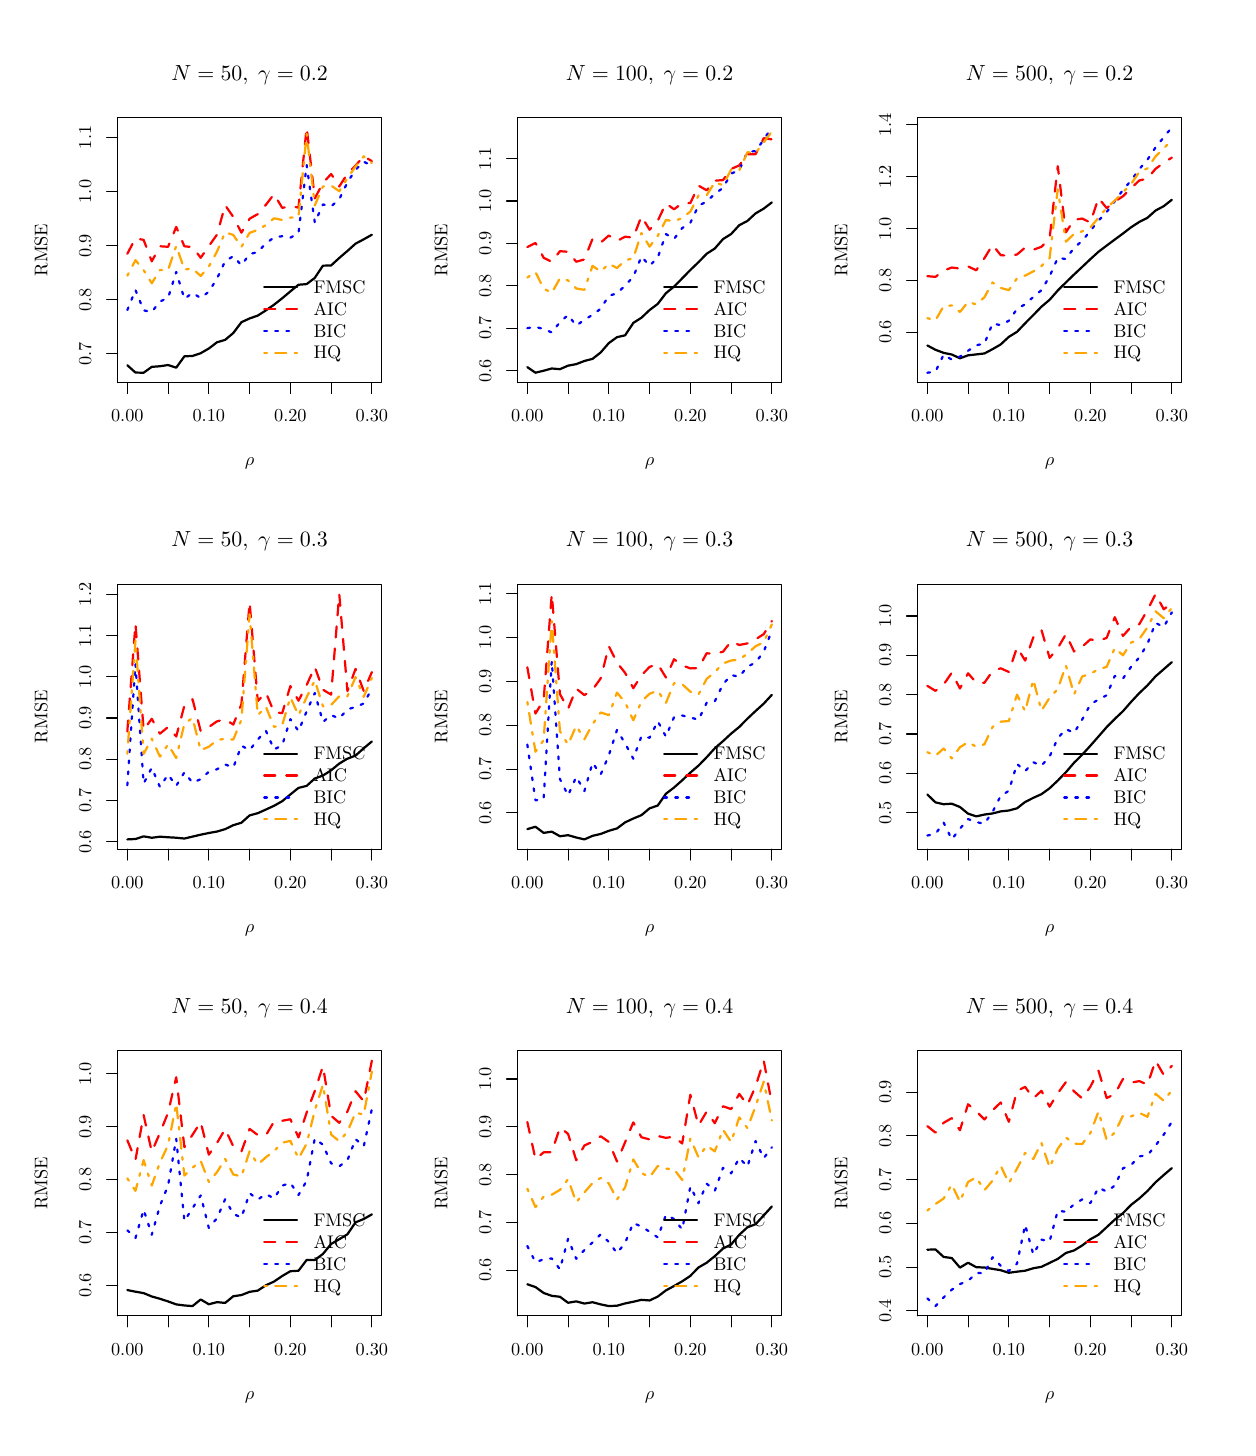
\begin{tikzpicture}[x=1pt,y=1pt]
\definecolor{fillColor}{RGB}{255,255,255}
\path[use as bounding box,fill=fillColor,fill opacity=0.00] (0,0) rectangle (433.62,505.89);
\begin{scope}
\path[clip] ( 32.47,377.65) rectangle (127.91,473.42);
\definecolor{drawColor}{RGB}{0,0,0}

\path[draw=drawColor,line width= 0.8pt,line join=round,line cap=round] ( 36.01,383.90) --
	( 38.95,381.26) --
	( 41.90,381.20) --
	( 44.84,383.32) --
	( 47.79,383.54) --
	( 50.73,383.98) --
	( 53.68,383.03) --
	( 56.63,387.12) --
	( 59.57,387.26) --
	( 62.52,388.26) --
	( 65.46,389.95) --
	( 68.41,392.20) --
	( 71.35,393.07) --
	( 74.30,395.55) --
	( 77.24,399.46) --
	( 80.19,400.81) --
	( 83.14,401.85) --
	( 86.08,403.72) --
	( 89.03,405.78) --
	( 91.97,408.10) --
	( 94.92,410.59) --
	( 97.86,412.99) --
	(100.81,413.23) --
	(103.75,415.46) --
	(106.70,419.88) --
	(109.65,419.97) --
	(112.59,422.67) --
	(115.54,425.20) --
	(118.48,427.84) --
	(121.43,429.40) --
	(124.37,431.06);
\end{scope}
\begin{scope}
\path[clip] (  0.00,  0.00) rectangle (433.62,505.89);
\definecolor{drawColor}{RGB}{0,0,0}

\path[draw=drawColor,line width= 0.4pt,line join=round,line cap=round] ( 36.01,377.65) -- (124.37,377.65);

\path[draw=drawColor,line width= 0.4pt,line join=round,line cap=round] ( 36.01,377.65) -- ( 36.01,373.69);

\path[draw=drawColor,line width= 0.4pt,line join=round,line cap=round] ( 50.73,377.65) -- ( 50.73,373.69);

\path[draw=drawColor,line width= 0.4pt,line join=round,line cap=round] ( 65.46,377.65) -- ( 65.46,373.69);

\path[draw=drawColor,line width= 0.4pt,line join=round,line cap=round] ( 80.19,377.65) -- ( 80.19,373.69);

\path[draw=drawColor,line width= 0.4pt,line join=round,line cap=round] ( 94.92,377.65) -- ( 94.92,373.69);

\path[draw=drawColor,line width= 0.4pt,line join=round,line cap=round] (109.65,377.65) -- (109.65,373.69);

\path[draw=drawColor,line width= 0.4pt,line join=round,line cap=round] (124.37,377.65) -- (124.37,373.69);

\node[text=drawColor,anchor=base,inner sep=0pt, outer sep=0pt, scale=  0.66] at ( 36.01,363.40) {0.00};

\node[text=drawColor,anchor=base,inner sep=0pt, outer sep=0pt, scale=  0.66] at ( 65.46,363.40) {0.10};

\node[text=drawColor,anchor=base,inner sep=0pt, outer sep=0pt, scale=  0.66] at ( 94.92,363.40) {0.20};

\node[text=drawColor,anchor=base,inner sep=0pt, outer sep=0pt, scale=  0.66] at (124.37,363.40) {0.30};

\path[draw=drawColor,line width= 0.4pt,line join=round,line cap=round] ( 32.47,388.00) -- ( 32.47,466.24);

\path[draw=drawColor,line width= 0.4pt,line join=round,line cap=round] ( 32.47,388.00) -- ( 28.51,388.00);

\path[draw=drawColor,line width= 0.4pt,line join=round,line cap=round] ( 32.47,407.56) -- ( 28.51,407.56);

\path[draw=drawColor,line width= 0.4pt,line join=round,line cap=round] ( 32.47,427.12) -- ( 28.51,427.12);

\path[draw=drawColor,line width= 0.4pt,line join=round,line cap=round] ( 32.47,446.68) -- ( 28.51,446.68);

\path[draw=drawColor,line width= 0.4pt,line join=round,line cap=round] ( 32.47,466.24) -- ( 28.51,466.24);

\node[text=drawColor,rotate= 90.00,anchor=base,inner sep=0pt, outer sep=0pt, scale=  0.66] at ( 22.97,388.00) {0.7};

\node[text=drawColor,rotate= 90.00,anchor=base,inner sep=0pt, outer sep=0pt, scale=  0.66] at ( 22.97,407.56) {0.8};

\node[text=drawColor,rotate= 90.00,anchor=base,inner sep=0pt, outer sep=0pt, scale=  0.66] at ( 22.97,427.12) {0.9};

\node[text=drawColor,rotate= 90.00,anchor=base,inner sep=0pt, outer sep=0pt, scale=  0.66] at ( 22.97,446.68) {1.0};

\node[text=drawColor,rotate= 90.00,anchor=base,inner sep=0pt, outer sep=0pt, scale=  0.66] at ( 22.97,466.24) {1.1};

\path[draw=drawColor,line width= 0.4pt,line join=round,line cap=round] ( 32.47,377.65) --
	(127.91,377.65) --
	(127.91,473.42) --
	( 32.47,473.42) --
	( 32.47,377.65);
\end{scope}
\begin{scope}
\path[clip] (  0.00,337.26) rectangle (144.54,505.89);
\definecolor{drawColor}{RGB}{0,0,0}

\node[text=drawColor,anchor=base,inner sep=0pt, outer sep=0pt, scale=  0.79] at ( 80.19,486.92) {\bfseries $N=50, \;\gamma=0.2$};

\node[text=drawColor,anchor=base,inner sep=0pt, outer sep=0pt, scale=  0.66] at ( 80.19,347.56) {$\rho$};

\node[text=drawColor,rotate= 90.00,anchor=base,inner sep=0pt, outer sep=0pt, scale=  0.66] at (  7.13,425.53) {RMSE};
\end{scope}
\begin{scope}
\path[clip] ( 32.47,377.65) rectangle (127.91,473.42);
\definecolor{drawColor}{RGB}{255,0,0}

\path[draw=drawColor,line width= 0.8pt,dash pattern=on 4pt off 4pt ,line join=round,line cap=round] ( 36.01,424.18) --
	( 38.95,429.77) --
	( 41.90,429.20) --
	( 44.84,421.45) --
	( 47.79,426.90) --
	( 50.73,426.70) --
	( 53.68,433.89) --
	( 56.63,426.88) --
	( 59.57,426.61) --
	( 62.52,422.74) --
	( 65.46,426.95) --
	( 68.41,431.10) --
	( 71.35,441.72) --
	( 74.30,437.51) --
	( 77.24,431.80) --
	( 80.19,436.85) --
	( 83.14,438.52) --
	( 86.08,441.88) --
	( 89.03,445.74) --
	( 91.97,440.78) --
	( 94.92,441.37) --
	( 97.86,440.88) --
	(100.81,469.87) --
	(103.75,444.20) --
	(106.70,449.78) --
	(109.65,453.03) --
	(112.59,448.49) --
	(115.54,453.11) --
	(118.48,456.06) --
	(121.43,459.42) --
	(124.37,457.67);
\definecolor{drawColor}{RGB}{0,0,255}

\path[draw=drawColor,line width= 0.8pt,dash pattern=on 1pt off 3pt ,line join=round,line cap=round] ( 36.01,403.85) --
	( 38.95,411.09) --
	( 41.90,403.74) --
	( 44.84,403.15) --
	( 47.79,406.94) --
	( 50.73,408.23) --
	( 53.68,417.61) --
	( 56.63,407.90) --
	( 59.57,410.05) --
	( 62.52,408.18) --
	( 65.46,410.49) --
	( 68.41,415.21) --
	( 71.35,421.50) --
	( 74.30,423.30) --
	( 77.24,420.02) --
	( 80.19,424.09) --
	( 83.14,424.77) --
	( 86.08,427.99) --
	( 89.03,430.05) --
	( 91.97,430.54) --
	( 94.92,430.01) --
	( 97.86,431.59) --
	(100.81,456.25) --
	(103.75,435.43) --
	(106.70,442.00) --
	(109.65,441.32) --
	(112.59,443.86) --
	(115.54,450.01) --
	(118.48,454.53) --
	(121.43,457.46) --
	(124.37,456.02);
\definecolor{drawColor}{RGB}{255,165,0}

\path[draw=drawColor,line width= 0.8pt,dash pattern=on 1pt off 3pt on 4pt off 3pt ,line join=round,line cap=round] ( 36.01,416.27) --
	( 38.95,421.87) --
	( 41.90,418.27) --
	( 44.84,413.52) --
	( 47.79,418.30) --
	( 50.73,418.29) --
	( 53.68,427.03) --
	( 56.63,418.49) --
	( 59.57,418.85) --
	( 62.52,416.15) --
	( 65.46,419.55) --
	( 68.41,424.98) --
	( 71.35,431.97) --
	( 74.30,430.96) --
	( 77.24,426.70) --
	( 80.19,431.74) --
	( 83.14,432.81) --
	( 86.08,434.56) --
	( 89.03,437.00) --
	( 91.97,436.41) --
	( 94.92,437.24) --
	( 97.86,437.55) --
	(100.81,467.50) --
	(103.75,441.70) --
	(106.70,448.50) --
	(109.65,448.82) --
	(112.59,446.79) --
	(115.54,451.50) --
	(118.48,455.71) --
	(121.43,459.40) --
	(124.37,456.98);
\definecolor{drawColor}{RGB}{0,0,0}

\path[draw=drawColor,line width= 0.8pt,line join=round,line cap=round] ( 85.47,412.20) -- ( 97.35,412.20);
\definecolor{drawColor}{RGB}{255,0,0}

\path[draw=drawColor,line width= 0.8pt,dash pattern=on 4pt off 4pt ,line join=round,line cap=round] ( 85.47,404.28) -- ( 97.35,404.28);
\definecolor{drawColor}{RGB}{0,0,255}

\path[draw=drawColor,line width= 0.8pt,dash pattern=on 1pt off 3pt ,line join=round,line cap=round] ( 85.47,396.36) -- ( 97.35,396.36);
\definecolor{drawColor}{RGB}{255,165,0}

\path[draw=drawColor,line width= 0.8pt,dash pattern=on 1pt off 3pt on 4pt off 3pt ,line join=round,line cap=round] ( 85.47,388.44) -- ( 97.35,388.44);
\definecolor{drawColor}{RGB}{0,0,0}

\node[text=drawColor,anchor=base west,inner sep=0pt, outer sep=0pt, scale=  0.66] at (103.29,409.93) {FMSC};

\node[text=drawColor,anchor=base west,inner sep=0pt, outer sep=0pt, scale=  0.66] at (103.29,402.01) {AIC};

\node[text=drawColor,anchor=base west,inner sep=0pt, outer sep=0pt, scale=  0.66] at (103.29,394.09) {BIC};

\node[text=drawColor,anchor=base west,inner sep=0pt, outer sep=0pt, scale=  0.66] at (103.29,386.17) {HQ};
\end{scope}
\begin{scope}
\path[clip] (177.01,377.65) rectangle (272.45,473.42);
\definecolor{drawColor}{RGB}{0,0,0}

\path[draw=drawColor,line width= 0.8pt,line join=round,line cap=round] (180.55,383.22) --
	(183.49,381.20) --
	(186.44,381.93) --
	(189.38,382.73) --
	(192.33,382.48) --
	(195.27,383.76) --
	(198.22,384.30) --
	(201.17,385.45) --
	(204.11,386.21) --
	(207.06,388.53) --
	(210.00,391.92) --
	(212.95,394.04) --
	(215.89,394.72) --
	(218.84,399.20) --
	(221.78,401.07) --
	(224.73,403.86) --
	(227.68,406.07) --
	(230.62,409.93) --
	(233.57,412.33) --
	(236.51,415.30) --
	(239.46,418.33) --
	(242.40,421.14) --
	(245.35,424.19) --
	(248.29,426.08) --
	(251.24,429.47) --
	(254.19,431.32) --
	(257.13,434.51) --
	(260.08,436.05) --
	(263.02,438.77) --
	(265.97,440.49) --
	(268.91,442.76);
\end{scope}
\begin{scope}
\path[clip] (  0.00,  0.00) rectangle (433.62,505.89);
\definecolor{drawColor}{RGB}{0,0,0}

\path[draw=drawColor,line width= 0.4pt,line join=round,line cap=round] (180.55,377.65) -- (268.91,377.65);

\path[draw=drawColor,line width= 0.4pt,line join=round,line cap=round] (180.55,377.65) -- (180.55,373.69);

\path[draw=drawColor,line width= 0.4pt,line join=round,line cap=round] (195.27,377.65) -- (195.27,373.69);

\path[draw=drawColor,line width= 0.4pt,line join=round,line cap=round] (210.00,377.65) -- (210.00,373.69);

\path[draw=drawColor,line width= 0.4pt,line join=round,line cap=round] (224.73,377.65) -- (224.73,373.69);

\path[draw=drawColor,line width= 0.4pt,line join=round,line cap=round] (239.46,377.65) -- (239.46,373.69);

\path[draw=drawColor,line width= 0.4pt,line join=round,line cap=round] (254.19,377.65) -- (254.19,373.69);

\path[draw=drawColor,line width= 0.4pt,line join=round,line cap=round] (268.91,377.65) -- (268.91,373.69);

\node[text=drawColor,anchor=base,inner sep=0pt, outer sep=0pt, scale=  0.66] at (180.55,363.40) {0.00};

\node[text=drawColor,anchor=base,inner sep=0pt, outer sep=0pt, scale=  0.66] at (210.00,363.40) {0.10};

\node[text=drawColor,anchor=base,inner sep=0pt, outer sep=0pt, scale=  0.66] at (239.46,363.40) {0.20};

\node[text=drawColor,anchor=base,inner sep=0pt, outer sep=0pt, scale=  0.66] at (268.91,363.40) {0.30};

\path[draw=drawColor,line width= 0.4pt,line join=round,line cap=round] (177.01,381.99) -- (177.01,458.56);

\path[draw=drawColor,line width= 0.4pt,line join=round,line cap=round] (177.01,381.99) -- (173.05,381.99);

\path[draw=drawColor,line width= 0.4pt,line join=round,line cap=round] (177.01,397.30) -- (173.05,397.30);

\path[draw=drawColor,line width= 0.4pt,line join=round,line cap=round] (177.01,412.62) -- (173.05,412.62);

\path[draw=drawColor,line width= 0.4pt,line join=round,line cap=round] (177.01,427.93) -- (173.05,427.93);

\path[draw=drawColor,line width= 0.4pt,line join=round,line cap=round] (177.01,443.25) -- (173.05,443.25);

\path[draw=drawColor,line width= 0.4pt,line join=round,line cap=round] (177.01,458.56) -- (173.05,458.56);

\node[text=drawColor,rotate= 90.00,anchor=base,inner sep=0pt, outer sep=0pt, scale=  0.66] at (167.51,381.99) {0.6};

\node[text=drawColor,rotate= 90.00,anchor=base,inner sep=0pt, outer sep=0pt, scale=  0.66] at (167.51,397.30) {0.7};

\node[text=drawColor,rotate= 90.00,anchor=base,inner sep=0pt, outer sep=0pt, scale=  0.66] at (167.51,412.62) {0.8};

\node[text=drawColor,rotate= 90.00,anchor=base,inner sep=0pt, outer sep=0pt, scale=  0.66] at (167.51,427.93) {0.9};

\node[text=drawColor,rotate= 90.00,anchor=base,inner sep=0pt, outer sep=0pt, scale=  0.66] at (167.51,443.25) {1.0};

\node[text=drawColor,rotate= 90.00,anchor=base,inner sep=0pt, outer sep=0pt, scale=  0.66] at (167.51,458.56) {1.1};

\path[draw=drawColor,line width= 0.4pt,line join=round,line cap=round] (177.01,377.65) --
	(272.45,377.65) --
	(272.45,473.42) --
	(177.01,473.42) --
	(177.01,377.65);
\end{scope}
\begin{scope}
\path[clip] (144.54,337.26) rectangle (289.08,505.89);
\definecolor{drawColor}{RGB}{0,0,0}

\node[text=drawColor,anchor=base,inner sep=0pt, outer sep=0pt, scale=  0.79] at (224.73,486.92) {\bfseries $N=100, \;\gamma=0.2$};

\node[text=drawColor,anchor=base,inner sep=0pt, outer sep=0pt, scale=  0.66] at (224.73,347.56) {$\rho$};

\node[text=drawColor,rotate= 90.00,anchor=base,inner sep=0pt, outer sep=0pt, scale=  0.66] at (151.67,425.53) {RMSE};
\end{scope}
\begin{scope}
\path[clip] (177.01,377.65) rectangle (272.45,473.42);
\definecolor{drawColor}{RGB}{255,0,0}

\path[draw=drawColor,line width= 0.8pt,dash pattern=on 4pt off 4pt ,line join=round,line cap=round] (180.55,426.60) --
	(183.49,428.10) --
	(186.44,422.76) --
	(189.38,421.25) --
	(192.33,425.13) --
	(195.27,424.89) --
	(198.22,421.31) --
	(201.17,422.14) --
	(204.11,429.57) --
	(207.06,428.22) --
	(210.00,430.78) --
	(212.95,428.79) --
	(215.89,430.36) --
	(218.84,430.00) --
	(221.78,437.73) --
	(224.73,432.88) --
	(227.68,436.12) --
	(230.62,442.36) --
	(233.57,440.26) --
	(236.51,442.48) --
	(239.46,442.51) --
	(242.40,448.81) --
	(245.35,447.12) --
	(248.29,450.60) --
	(251.24,450.80) --
	(254.19,454.83) --
	(257.13,456.12) --
	(260.08,460.11) --
	(263.02,460.16) --
	(265.97,465.94) --
	(268.91,465.51);
\definecolor{drawColor}{RGB}{0,0,255}

\path[draw=drawColor,line width= 0.8pt,dash pattern=on 1pt off 3pt ,line join=round,line cap=round] (180.55,397.32) --
	(183.49,397.71) --
	(186.44,397.06) --
	(189.38,395.74) --
	(192.33,399.47) --
	(195.27,402.07) --
	(198.22,398.22) --
	(201.17,400.33) --
	(204.11,402.11) --
	(207.06,404.33) --
	(210.00,409.04) --
	(212.95,409.85) --
	(215.89,412.72) --
	(218.84,415.83) --
	(221.78,423.21) --
	(224.73,419.85) --
	(227.68,422.81) --
	(230.62,431.31) --
	(233.57,429.55) --
	(236.51,433.47) --
	(239.46,435.38) --
	(242.40,441.57) --
	(245.35,443.05) --
	(248.29,445.82) --
	(251.24,447.99) --
	(254.19,453.16) --
	(257.13,454.38) --
	(260.08,461.06) --
	(263.02,461.25) --
	(265.97,465.44) --
	(268.91,469.87);
\definecolor{drawColor}{RGB}{255,165,0}

\path[draw=drawColor,line width= 0.8pt,dash pattern=on 1pt off 3pt on 4pt off 3pt ,line join=round,line cap=round] (180.55,415.59) --
	(183.49,417.56) --
	(186.44,411.60) --
	(189.38,410.05) --
	(192.33,415.30) --
	(195.27,414.55) --
	(198.22,411.64) --
	(201.17,411.16) --
	(204.11,419.82) --
	(207.06,417.72) --
	(210.00,420.58) --
	(212.95,419.03) --
	(215.89,421.79) --
	(218.84,422.58) --
	(221.78,431.67) --
	(224.73,426.75) --
	(227.68,430.69) --
	(230.62,436.38) --
	(233.57,435.95) --
	(236.51,437.12) --
	(239.46,439.44) --
	(242.40,445.22) --
	(245.35,445.33) --
	(248.29,450.01) --
	(251.24,448.97) --
	(254.19,454.56) --
	(257.13,454.30) --
	(260.08,460.89) --
	(263.02,460.59) --
	(265.97,464.44) --
	(268.91,468.34);
\definecolor{drawColor}{RGB}{0,0,0}

\path[draw=drawColor,line width= 0.8pt,line join=round,line cap=round] (230.01,412.20) -- (241.89,412.20);
\definecolor{drawColor}{RGB}{255,0,0}

\path[draw=drawColor,line width= 0.8pt,dash pattern=on 4pt off 4pt ,line join=round,line cap=round] (230.01,404.28) -- (241.89,404.28);
\definecolor{drawColor}{RGB}{0,0,255}

\path[draw=drawColor,line width= 0.8pt,dash pattern=on 1pt off 3pt ,line join=round,line cap=round] (230.01,396.36) -- (241.89,396.36);
\definecolor{drawColor}{RGB}{255,165,0}

\path[draw=drawColor,line width= 0.8pt,dash pattern=on 1pt off 3pt on 4pt off 3pt ,line join=round,line cap=round] (230.01,388.44) -- (241.89,388.44);
\definecolor{drawColor}{RGB}{0,0,0}

\node[text=drawColor,anchor=base west,inner sep=0pt, outer sep=0pt, scale=  0.66] at (247.83,409.93) {FMSC};

\node[text=drawColor,anchor=base west,inner sep=0pt, outer sep=0pt, scale=  0.66] at (247.83,402.01) {AIC};

\node[text=drawColor,anchor=base west,inner sep=0pt, outer sep=0pt, scale=  0.66] at (247.83,394.09) {BIC};

\node[text=drawColor,anchor=base west,inner sep=0pt, outer sep=0pt, scale=  0.66] at (247.83,386.17) {HQ};
\end{scope}
\begin{scope}
\path[clip] (321.55,377.65) rectangle (416.99,473.42);
\definecolor{drawColor}{RGB}{0,0,0}

\path[draw=drawColor,line width= 0.8pt,line join=round,line cap=round] (325.09,391.05) --
	(328.03,389.49) --
	(330.98,388.38) --
	(333.92,387.78) --
	(336.87,386.42) --
	(339.81,387.48) --
	(342.76,387.82) --
	(345.71,388.16) --
	(348.65,389.71) --
	(351.60,391.43) --
	(354.54,394.16) --
	(357.49,395.97) --
	(360.43,399.06) --
	(363.38,402.03) --
	(366.32,405.06) --
	(369.27,407.55) --
	(372.22,410.91) --
	(375.16,413.83) --
	(378.11,416.69) --
	(381.05,419.44) --
	(384.00,422.23) --
	(386.94,424.91) --
	(389.89,427.14) --
	(392.83,429.33) --
	(395.78,431.50) --
	(398.73,433.77) --
	(401.67,435.68) --
	(404.62,437.18) --
	(407.56,439.81) --
	(410.51,441.38) --
	(413.45,443.70);
\end{scope}
\begin{scope}
\path[clip] (  0.00,  0.00) rectangle (433.62,505.89);
\definecolor{drawColor}{RGB}{0,0,0}

\path[draw=drawColor,line width= 0.4pt,line join=round,line cap=round] (325.09,377.65) -- (413.45,377.65);

\path[draw=drawColor,line width= 0.4pt,line join=round,line cap=round] (325.09,377.65) -- (325.09,373.69);

\path[draw=drawColor,line width= 0.4pt,line join=round,line cap=round] (339.81,377.65) -- (339.81,373.69);

\path[draw=drawColor,line width= 0.4pt,line join=round,line cap=round] (354.54,377.65) -- (354.54,373.69);

\path[draw=drawColor,line width= 0.4pt,line join=round,line cap=round] (369.27,377.65) -- (369.27,373.69);

\path[draw=drawColor,line width= 0.4pt,line join=round,line cap=round] (384.00,377.65) -- (384.00,373.69);

\path[draw=drawColor,line width= 0.4pt,line join=round,line cap=round] (398.73,377.65) -- (398.73,373.69);

\path[draw=drawColor,line width= 0.4pt,line join=round,line cap=round] (413.45,377.65) -- (413.45,373.69);

\node[text=drawColor,anchor=base,inner sep=0pt, outer sep=0pt, scale=  0.66] at (325.09,363.40) {0.00};

\node[text=drawColor,anchor=base,inner sep=0pt, outer sep=0pt, scale=  0.66] at (354.54,363.40) {0.10};

\node[text=drawColor,anchor=base,inner sep=0pt, outer sep=0pt, scale=  0.66] at (384.00,363.40) {0.20};

\node[text=drawColor,anchor=base,inner sep=0pt, outer sep=0pt, scale=  0.66] at (413.45,363.40) {0.30};

\path[draw=drawColor,line width= 0.4pt,line join=round,line cap=round] (321.55,395.84) -- (321.55,470.76);

\path[draw=drawColor,line width= 0.4pt,line join=round,line cap=round] (321.55,395.84) -- (317.59,395.84);

\path[draw=drawColor,line width= 0.4pt,line join=round,line cap=round] (321.55,414.57) -- (317.59,414.57);

\path[draw=drawColor,line width= 0.4pt,line join=round,line cap=round] (321.55,433.30) -- (317.59,433.30);

\path[draw=drawColor,line width= 0.4pt,line join=round,line cap=round] (321.55,452.03) -- (317.59,452.03);

\path[draw=drawColor,line width= 0.4pt,line join=round,line cap=round] (321.55,470.76) -- (317.59,470.76);

\node[text=drawColor,rotate= 90.00,anchor=base,inner sep=0pt, outer sep=0pt, scale=  0.66] at (312.05,395.84) {0.6};

\node[text=drawColor,rotate= 90.00,anchor=base,inner sep=0pt, outer sep=0pt, scale=  0.66] at (312.05,414.57) {0.8};

\node[text=drawColor,rotate= 90.00,anchor=base,inner sep=0pt, outer sep=0pt, scale=  0.66] at (312.05,433.30) {1.0};

\node[text=drawColor,rotate= 90.00,anchor=base,inner sep=0pt, outer sep=0pt, scale=  0.66] at (312.05,452.03) {1.2};

\node[text=drawColor,rotate= 90.00,anchor=base,inner sep=0pt, outer sep=0pt, scale=  0.66] at (312.05,470.76) {1.4};

\path[draw=drawColor,line width= 0.4pt,line join=round,line cap=round] (321.55,377.65) --
	(416.99,377.65) --
	(416.99,473.42) --
	(321.55,473.42) --
	(321.55,377.65);
\end{scope}
\begin{scope}
\path[clip] (289.08,337.26) rectangle (433.62,505.89);
\definecolor{drawColor}{RGB}{0,0,0}

\node[text=drawColor,anchor=base,inner sep=0pt, outer sep=0pt, scale=  0.79] at (369.27,486.92) {\bfseries $N=500, \;\gamma=0.2$};

\node[text=drawColor,anchor=base,inner sep=0pt, outer sep=0pt, scale=  0.66] at (369.27,347.56) {$\rho$};

\node[text=drawColor,rotate= 90.00,anchor=base,inner sep=0pt, outer sep=0pt, scale=  0.66] at (296.21,425.53) {RMSE};
\end{scope}
\begin{scope}
\path[clip] (321.55,377.65) rectangle (416.99,473.42);
\definecolor{drawColor}{RGB}{255,0,0}

\path[draw=drawColor,line width= 0.8pt,dash pattern=on 4pt off 4pt ,line join=round,line cap=round] (325.09,416.10) --
	(328.03,415.84) --
	(330.98,418.10) --
	(333.92,419.21) --
	(336.87,418.86) --
	(339.81,419.61) --
	(342.76,418.22) --
	(345.71,422.57) --
	(348.65,427.41) --
	(351.60,423.69) --
	(354.54,423.44) --
	(357.49,423.91) --
	(360.43,426.43) --
	(363.38,425.64) --
	(366.32,426.70) --
	(369.27,429.70) --
	(372.22,455.84) --
	(375.16,431.93) --
	(378.11,436.46) --
	(381.05,436.91) --
	(384.00,435.48) --
	(386.94,444.34) --
	(389.89,440.69) --
	(392.83,443.10) --
	(395.78,444.95) --
	(398.73,447.89) --
	(401.67,450.67) --
	(404.62,451.37) --
	(407.56,454.89) --
	(410.51,457.04) --
	(413.45,458.94);
\definecolor{drawColor}{RGB}{0,0,255}

\path[draw=drawColor,line width= 0.8pt,dash pattern=on 1pt off 3pt ,line join=round,line cap=round] (325.09,381.20) --
	(328.03,381.58) --
	(330.98,387.75) --
	(333.92,385.92) --
	(336.87,387.01) --
	(339.81,389.13) --
	(342.76,391.14) --
	(345.71,391.68) --
	(348.65,398.99) --
	(351.60,398.39) --
	(354.54,400.00) --
	(357.49,404.23) --
	(360.43,405.95) --
	(363.38,408.59) --
	(366.32,411.03) --
	(369.27,416.01) --
	(372.22,422.71) --
	(375.16,422.28) --
	(378.11,426.34) --
	(381.05,428.85) --
	(384.00,432.49) --
	(386.94,436.19) --
	(389.89,439.25) --
	(392.83,443.18) --
	(395.78,447.26) --
	(398.73,450.63) --
	(401.67,454.75) --
	(404.62,458.17) --
	(407.56,462.62) --
	(410.51,466.29) --
	(413.45,469.87);
\definecolor{drawColor}{RGB}{255,165,0}

\path[draw=drawColor,line width= 0.8pt,dash pattern=on 1pt off 3pt on 4pt off 3pt ,line join=round,line cap=round] (325.09,400.92) --
	(328.03,400.15) --
	(330.98,405.26) --
	(333.92,405.50) --
	(336.87,403.15) --
	(339.81,406.76) --
	(342.76,405.89) --
	(345.71,408.47) --
	(348.65,413.79) --
	(351.60,411.85) --
	(354.54,411.04) --
	(357.49,415.31) --
	(360.43,416.30) --
	(363.38,417.80) --
	(366.32,419.76) --
	(369.27,422.64) --
	(372.22,447.49) --
	(375.16,428.54) --
	(378.11,431.37) --
	(381.05,432.28) --
	(384.00,433.72) --
	(386.94,437.21) --
	(389.89,440.77) --
	(392.83,443.40) --
	(395.78,446.37) --
	(398.73,449.39) --
	(401.67,453.74) --
	(404.62,455.04) --
	(407.56,459.37) --
	(410.51,462.23) --
	(413.45,465.36);
\definecolor{drawColor}{RGB}{0,0,0}

\path[draw=drawColor,line width= 0.8pt,line join=round,line cap=round] (374.55,412.20) -- (386.43,412.20);
\definecolor{drawColor}{RGB}{255,0,0}

\path[draw=drawColor,line width= 0.8pt,dash pattern=on 4pt off 4pt ,line join=round,line cap=round] (374.55,404.28) -- (386.43,404.28);
\definecolor{drawColor}{RGB}{0,0,255}

\path[draw=drawColor,line width= 0.8pt,dash pattern=on 1pt off 3pt ,line join=round,line cap=round] (374.55,396.36) -- (386.43,396.36);
\definecolor{drawColor}{RGB}{255,165,0}

\path[draw=drawColor,line width= 0.8pt,dash pattern=on 1pt off 3pt on 4pt off 3pt ,line join=round,line cap=round] (374.55,388.44) -- (386.43,388.44);
\definecolor{drawColor}{RGB}{0,0,0}

\node[text=drawColor,anchor=base west,inner sep=0pt, outer sep=0pt, scale=  0.66] at (392.37,409.93) {FMSC};

\node[text=drawColor,anchor=base west,inner sep=0pt, outer sep=0pt, scale=  0.66] at (392.37,402.01) {AIC};

\node[text=drawColor,anchor=base west,inner sep=0pt, outer sep=0pt, scale=  0.66] at (392.37,394.09) {BIC};

\node[text=drawColor,anchor=base west,inner sep=0pt, outer sep=0pt, scale=  0.66] at (392.37,386.17) {HQ};
\end{scope}
\begin{scope}
\path[clip] ( 32.47,209.02) rectangle (127.91,304.79);
\definecolor{drawColor}{RGB}{0,0,0}

\path[draw=drawColor,line width= 0.8pt,line join=round,line cap=round] ( 36.01,212.57) --
	( 38.95,212.71) --
	( 41.90,213.67) --
	( 44.84,213.16) --
	( 47.79,213.55) --
	( 50.73,213.34) --
	( 53.68,213.18) --
	( 56.63,212.88) --
	( 59.57,213.58) --
	( 62.52,214.27) --
	( 65.46,214.88) --
	( 68.41,215.41) --
	( 71.35,216.27) --
	( 74.30,217.70) --
	( 77.24,218.60) --
	( 80.19,221.24) --
	( 83.14,222.04) --
	( 86.08,223.36) --
	( 89.03,224.72) --
	( 91.97,226.37) --
	( 94.92,228.81) --
	( 97.86,231.18) --
	(100.81,231.91) --
	(103.75,234.58) --
	(106.70,235.65) --
	(109.65,237.53) --
	(112.59,239.97) --
	(115.54,241.73) --
	(118.48,242.86) --
	(121.43,245.50) --
	(124.37,247.95);
\end{scope}
\begin{scope}
\path[clip] (  0.00,  0.00) rectangle (433.62,505.89);
\definecolor{drawColor}{RGB}{0,0,0}

\path[draw=drawColor,line width= 0.4pt,line join=round,line cap=round] ( 36.01,209.02) -- (124.37,209.02);

\path[draw=drawColor,line width= 0.4pt,line join=round,line cap=round] ( 36.01,209.02) -- ( 36.01,205.06);

\path[draw=drawColor,line width= 0.4pt,line join=round,line cap=round] ( 50.73,209.02) -- ( 50.73,205.06);

\path[draw=drawColor,line width= 0.4pt,line join=round,line cap=round] ( 65.46,209.02) -- ( 65.46,205.06);

\path[draw=drawColor,line width= 0.4pt,line join=round,line cap=round] ( 80.19,209.02) -- ( 80.19,205.06);

\path[draw=drawColor,line width= 0.4pt,line join=round,line cap=round] ( 94.92,209.02) -- ( 94.92,205.06);

\path[draw=drawColor,line width= 0.4pt,line join=round,line cap=round] (109.65,209.02) -- (109.65,205.06);

\path[draw=drawColor,line width= 0.4pt,line join=round,line cap=round] (124.37,209.02) -- (124.37,205.06);

\node[text=drawColor,anchor=base,inner sep=0pt, outer sep=0pt, scale=  0.66] at ( 36.01,194.77) {0.00};

\node[text=drawColor,anchor=base,inner sep=0pt, outer sep=0pt, scale=  0.66] at ( 65.46,194.77) {0.10};

\node[text=drawColor,anchor=base,inner sep=0pt, outer sep=0pt, scale=  0.66] at ( 94.92,194.77) {0.20};

\node[text=drawColor,anchor=base,inner sep=0pt, outer sep=0pt, scale=  0.66] at (124.37,194.77) {0.30};

\path[draw=drawColor,line width= 0.4pt,line join=round,line cap=round] ( 32.47,211.73) -- ( 32.47,301.11);

\path[draw=drawColor,line width= 0.4pt,line join=round,line cap=round] ( 32.47,211.73) -- ( 28.51,211.73);

\path[draw=drawColor,line width= 0.4pt,line join=round,line cap=round] ( 32.47,226.63) -- ( 28.51,226.63);

\path[draw=drawColor,line width= 0.4pt,line join=round,line cap=round] ( 32.47,241.52) -- ( 28.51,241.52);

\path[draw=drawColor,line width= 0.4pt,line join=round,line cap=round] ( 32.47,256.42) -- ( 28.51,256.42);

\path[draw=drawColor,line width= 0.4pt,line join=round,line cap=round] ( 32.47,271.32) -- ( 28.51,271.32);

\path[draw=drawColor,line width= 0.4pt,line join=round,line cap=round] ( 32.47,286.22) -- ( 28.51,286.22);

\path[draw=drawColor,line width= 0.4pt,line join=round,line cap=round] ( 32.47,301.11) -- ( 28.51,301.11);

\node[text=drawColor,rotate= 90.00,anchor=base,inner sep=0pt, outer sep=0pt, scale=  0.66] at ( 22.97,211.73) {0.6};

\node[text=drawColor,rotate= 90.00,anchor=base,inner sep=0pt, outer sep=0pt, scale=  0.66] at ( 22.97,226.63) {0.7};

\node[text=drawColor,rotate= 90.00,anchor=base,inner sep=0pt, outer sep=0pt, scale=  0.66] at ( 22.97,241.52) {0.8};

\node[text=drawColor,rotate= 90.00,anchor=base,inner sep=0pt, outer sep=0pt, scale=  0.66] at ( 22.97,256.42) {0.9};

\node[text=drawColor,rotate= 90.00,anchor=base,inner sep=0pt, outer sep=0pt, scale=  0.66] at ( 22.97,271.32) {1.0};

\node[text=drawColor,rotate= 90.00,anchor=base,inner sep=0pt, outer sep=0pt, scale=  0.66] at ( 22.97,286.22) {1.1};

\node[text=drawColor,rotate= 90.00,anchor=base,inner sep=0pt, outer sep=0pt, scale=  0.66] at ( 22.97,301.11) {1.2};

\path[draw=drawColor,line width= 0.4pt,line join=round,line cap=round] ( 32.47,209.02) --
	(127.91,209.02) --
	(127.91,304.79) --
	( 32.47,304.79) --
	( 32.47,209.02);
\end{scope}
\begin{scope}
\path[clip] (  0.00,168.63) rectangle (144.54,337.26);
\definecolor{drawColor}{RGB}{0,0,0}

\node[text=drawColor,anchor=base,inner sep=0pt, outer sep=0pt, scale=  0.79] at ( 80.19,318.29) {\bfseries $N=50, \;\gamma=0.3$};

\node[text=drawColor,anchor=base,inner sep=0pt, outer sep=0pt, scale=  0.66] at ( 80.19,178.93) {$\rho$};

\node[text=drawColor,rotate= 90.00,anchor=base,inner sep=0pt, outer sep=0pt, scale=  0.66] at (  7.13,256.90) {RMSE};
\end{scope}
\begin{scope}
\path[clip] ( 32.47,209.02) rectangle (127.91,304.79);
\definecolor{drawColor}{RGB}{255,0,0}

\path[draw=drawColor,line width= 0.8pt,dash pattern=on 4pt off 4pt ,line join=round,line cap=round] ( 36.01,251.58) --
	( 38.95,290.52) --
	( 41.90,252.15) --
	( 44.84,256.15) --
	( 47.79,250.78) --
	( 50.73,253.19) --
	( 53.68,249.76) --
	( 56.63,260.91) --
	( 59.57,263.21) --
	( 62.52,251.72) --
	( 65.46,253.20) --
	( 68.41,255.23) --
	( 71.35,255.97) --
	( 74.30,254.06) --
	( 77.24,261.42) --
	( 80.19,298.32) --
	( 83.14,262.55) --
	( 86.08,265.62) --
	( 89.03,258.54) --
	( 91.97,258.19) --
	( 94.92,267.99) --
	( 97.86,262.69) --
	(100.81,268.35) --
	(103.75,274.89) --
	(106.70,266.66) --
	(109.65,264.88) --
	(112.59,301.24) --
	(115.54,266.15) --
	(118.48,274.19) --
	(121.43,266.18) --
	(124.37,273.03);
\definecolor{drawColor}{RGB}{0,0,255}

\path[draw=drawColor,line width= 0.8pt,dash pattern=on 1pt off 3pt ,line join=round,line cap=round] ( 36.01,232.13) --
	( 38.95,275.94) --
	( 41.90,232.75) --
	( 44.84,238.46) --
	( 47.79,231.51) --
	( 50.73,236.00) --
	( 53.68,231.92) --
	( 56.63,236.82) --
	( 59.57,233.02) --
	( 62.52,234.35) --
	( 65.46,237.01) --
	( 68.41,237.92) --
	( 71.35,239.66) --
	( 74.30,238.55) --
	( 77.24,246.45) --
	( 80.19,244.80) --
	( 83.14,248.64) --
	( 86.08,251.82) --
	( 89.03,245.08) --
	( 91.97,246.58) --
	( 94.92,256.01) --
	( 97.86,251.73) --
	(100.81,258.84) --
	(103.75,265.46) --
	(106.70,255.02) --
	(109.65,257.49) --
	(112.59,256.25) --
	(115.54,259.58) --
	(118.48,260.41) --
	(121.43,261.67) --
	(124.37,267.02);
\definecolor{drawColor}{RGB}{255,165,0}

\path[draw=drawColor,line width= 0.8pt,dash pattern=on 1pt off 3pt on 4pt off 3pt ,line join=round,line cap=round] ( 36.01,243.55) --
	( 38.95,284.38) --
	( 41.90,243.43) --
	( 44.84,248.96) --
	( 47.79,242.48) --
	( 50.73,246.89) --
	( 53.68,241.97) --
	( 56.63,254.39) --
	( 59.57,256.44) --
	( 62.52,244.77) --
	( 65.46,246.06) --
	( 68.41,248.42) --
	( 71.35,248.96) --
	( 74.30,248.62) --
	( 77.24,255.85) --
	( 80.19,293.92) --
	( 83.14,257.45) --
	( 86.08,260.49) --
	( 89.03,253.24) --
	( 91.97,253.86) --
	( 94.92,263.92) --
	( 97.86,257.40) --
	(100.81,263.98) --
	(103.75,270.03) --
	(106.70,260.65) --
	(109.65,261.15) --
	(112.59,264.31) --
	(115.54,264.27) --
	(118.48,271.23) --
	(121.43,264.08) --
	(124.37,270.91);
\definecolor{drawColor}{RGB}{0,0,0}

\path[draw=drawColor,line width= 0.8pt,line join=round,line cap=round] ( 85.47,243.57) -- ( 97.35,243.57);
\definecolor{drawColor}{RGB}{255,0,0}

\path[draw=drawColor,line width= 0.8pt,dash pattern=on 4pt off 4pt ,line join=round,line cap=round] ( 85.47,235.65) -- ( 97.35,235.65);
\definecolor{drawColor}{RGB}{0,0,255}

\path[draw=drawColor,line width= 0.8pt,dash pattern=on 1pt off 3pt ,line join=round,line cap=round] ( 85.47,227.73) -- ( 97.35,227.73);
\definecolor{drawColor}{RGB}{255,165,0}

\path[draw=drawColor,line width= 0.8pt,dash pattern=on 1pt off 3pt on 4pt off 3pt ,line join=round,line cap=round] ( 85.47,219.81) -- ( 97.35,219.81);
\definecolor{drawColor}{RGB}{0,0,0}

\node[text=drawColor,anchor=base west,inner sep=0pt, outer sep=0pt, scale=  0.66] at (103.29,241.30) {FMSC};

\node[text=drawColor,anchor=base west,inner sep=0pt, outer sep=0pt, scale=  0.66] at (103.29,233.38) {AIC};

\node[text=drawColor,anchor=base west,inner sep=0pt, outer sep=0pt, scale=  0.66] at (103.29,225.46) {BIC};

\node[text=drawColor,anchor=base west,inner sep=0pt, outer sep=0pt, scale=  0.66] at (103.29,217.54) {HQ};
\end{scope}
\begin{scope}
\path[clip] (177.01,209.02) rectangle (272.45,304.79);
\definecolor{drawColor}{RGB}{0,0,0}

\path[draw=drawColor,line width= 0.8pt,line join=round,line cap=round] (180.55,216.28) --
	(183.49,217.14) --
	(186.44,214.92) --
	(189.38,215.37) --
	(192.33,213.71) --
	(195.27,214.09) --
	(198.22,213.26) --
	(201.17,212.57) --
	(204.11,213.85) --
	(207.06,214.54) --
	(210.00,215.67) --
	(212.95,216.53) --
	(215.89,218.73) --
	(218.84,220.11) --
	(221.78,221.33) --
	(224.73,223.79) --
	(227.68,224.81) --
	(230.62,229.06) --
	(233.57,231.32) --
	(236.51,233.93) --
	(239.46,236.70) --
	(242.40,239.23) --
	(245.35,242.25) --
	(248.29,245.50) --
	(251.24,248.06) --
	(254.19,250.79) --
	(257.13,253.20) --
	(260.08,256.19) --
	(263.02,258.96) --
	(265.97,261.62) --
	(268.91,264.81);
\end{scope}
\begin{scope}
\path[clip] (  0.00,  0.00) rectangle (433.62,505.89);
\definecolor{drawColor}{RGB}{0,0,0}

\path[draw=drawColor,line width= 0.4pt,line join=round,line cap=round] (180.55,209.02) -- (268.91,209.02);

\path[draw=drawColor,line width= 0.4pt,line join=round,line cap=round] (180.55,209.02) -- (180.55,205.06);

\path[draw=drawColor,line width= 0.4pt,line join=round,line cap=round] (195.27,209.02) -- (195.27,205.06);

\path[draw=drawColor,line width= 0.4pt,line join=round,line cap=round] (210.00,209.02) -- (210.00,205.06);

\path[draw=drawColor,line width= 0.4pt,line join=round,line cap=round] (224.73,209.02) -- (224.73,205.06);

\path[draw=drawColor,line width= 0.4pt,line join=round,line cap=round] (239.46,209.02) -- (239.46,205.06);

\path[draw=drawColor,line width= 0.4pt,line join=round,line cap=round] (254.19,209.02) -- (254.19,205.06);

\path[draw=drawColor,line width= 0.4pt,line join=round,line cap=round] (268.91,209.02) -- (268.91,205.06);

\node[text=drawColor,anchor=base,inner sep=0pt, outer sep=0pt, scale=  0.66] at (180.55,194.77) {0.00};

\node[text=drawColor,anchor=base,inner sep=0pt, outer sep=0pt, scale=  0.66] at (210.00,194.77) {0.10};

\node[text=drawColor,anchor=base,inner sep=0pt, outer sep=0pt, scale=  0.66] at (239.46,194.77) {0.20};

\node[text=drawColor,anchor=base,inner sep=0pt, outer sep=0pt, scale=  0.66] at (268.91,194.77) {0.30};

\path[draw=drawColor,line width= 0.4pt,line join=round,line cap=round] (177.01,222.14) -- (177.01,301.37);

\path[draw=drawColor,line width= 0.4pt,line join=round,line cap=round] (177.01,222.14) -- (173.05,222.14);

\path[draw=drawColor,line width= 0.4pt,line join=round,line cap=round] (177.01,237.98) -- (173.05,237.98);

\path[draw=drawColor,line width= 0.4pt,line join=round,line cap=round] (177.01,253.83) -- (173.05,253.83);

\path[draw=drawColor,line width= 0.4pt,line join=round,line cap=round] (177.01,269.68) -- (173.05,269.68);

\path[draw=drawColor,line width= 0.4pt,line join=round,line cap=round] (177.01,285.52) -- (173.05,285.52);

\path[draw=drawColor,line width= 0.4pt,line join=round,line cap=round] (177.01,301.37) -- (173.05,301.37);

\node[text=drawColor,rotate= 90.00,anchor=base,inner sep=0pt, outer sep=0pt, scale=  0.66] at (167.51,222.14) {0.6};

\node[text=drawColor,rotate= 90.00,anchor=base,inner sep=0pt, outer sep=0pt, scale=  0.66] at (167.51,237.98) {0.7};

\node[text=drawColor,rotate= 90.00,anchor=base,inner sep=0pt, outer sep=0pt, scale=  0.66] at (167.51,253.83) {0.8};

\node[text=drawColor,rotate= 90.00,anchor=base,inner sep=0pt, outer sep=0pt, scale=  0.66] at (167.51,269.68) {0.9};

\node[text=drawColor,rotate= 90.00,anchor=base,inner sep=0pt, outer sep=0pt, scale=  0.66] at (167.51,285.52) {1.0};

\node[text=drawColor,rotate= 90.00,anchor=base,inner sep=0pt, outer sep=0pt, scale=  0.66] at (167.51,301.37) {1.1};

\path[draw=drawColor,line width= 0.4pt,line join=round,line cap=round] (177.01,209.02) --
	(272.45,209.02) --
	(272.45,304.79) --
	(177.01,304.79) --
	(177.01,209.02);
\end{scope}
\begin{scope}
\path[clip] (144.54,168.63) rectangle (289.08,337.26);
\definecolor{drawColor}{RGB}{0,0,0}

\node[text=drawColor,anchor=base,inner sep=0pt, outer sep=0pt, scale=  0.79] at (224.73,318.29) {\bfseries $N=100, \;\gamma=0.3$};

\node[text=drawColor,anchor=base,inner sep=0pt, outer sep=0pt, scale=  0.66] at (224.73,178.93) {$\rho$};

\node[text=drawColor,rotate= 90.00,anchor=base,inner sep=0pt, outer sep=0pt, scale=  0.66] at (151.67,256.90) {RMSE};
\end{scope}
\begin{scope}
\path[clip] (177.01,209.02) rectangle (272.45,304.79);
\definecolor{drawColor}{RGB}{255,0,0}

\path[draw=drawColor,line width= 0.8pt,dash pattern=on 4pt off 4pt ,line join=round,line cap=round] (180.55,274.76) --
	(183.49,258.03) --
	(186.44,262.95) --
	(189.38,301.24) --
	(192.33,265.07) --
	(195.27,259.75) --
	(198.22,267.05) --
	(201.17,264.71) --
	(204.11,266.65) --
	(207.06,270.76) --
	(210.00,282.39) --
	(212.95,276.44) --
	(215.89,272.74) --
	(218.84,267.21) --
	(221.78,271.86) --
	(224.73,274.90) --
	(227.68,275.93) --
	(230.62,271.09) --
	(233.57,277.66) --
	(236.51,275.46) --
	(239.46,274.36) --
	(242.40,274.49) --
	(245.35,279.82) --
	(248.29,279.64) --
	(251.24,280.38) --
	(254.19,284.11) --
	(257.13,282.82) --
	(260.08,283.40) --
	(263.02,284.87) --
	(265.97,286.74) --
	(268.91,291.49);
\definecolor{drawColor}{RGB}{0,0,255}

\path[draw=drawColor,line width= 0.8pt,dash pattern=on 1pt off 3pt ,line join=round,line cap=round] (180.55,246.83) --
	(183.49,226.70) --
	(186.44,227.08) --
	(189.38,277.07) --
	(192.33,234.36) --
	(195.27,228.47) --
	(198.22,235.18) --
	(201.17,230.04) --
	(204.11,240.24) --
	(207.06,236.03) --
	(210.00,242.96) --
	(212.95,252.12) --
	(215.89,247.25) --
	(218.84,241.73) --
	(221.78,249.83) --
	(224.73,249.30) --
	(227.68,255.27) --
	(230.62,249.73) --
	(233.57,256.76) --
	(236.51,257.33) --
	(239.46,256.65) --
	(242.40,255.78) --
	(245.35,261.92) --
	(248.29,262.47) --
	(251.24,268.61) --
	(254.19,271.96) --
	(257.13,271.34) --
	(260.08,274.99) --
	(263.02,276.45) --
	(265.97,280.42) --
	(268.91,288.03);
\definecolor{drawColor}{RGB}{255,165,0}

\path[draw=drawColor,line width= 0.8pt,dash pattern=on 1pt off 3pt on 4pt off 3pt ,line join=round,line cap=round] (180.55,262.24) --
	(183.49,244.25) --
	(186.44,248.40) --
	(189.38,291.43) --
	(192.33,251.67) --
	(195.27,246.82) --
	(198.22,253.62) --
	(201.17,248.72) --
	(204.11,254.20) --
	(207.06,258.44) --
	(210.00,257.45) --
	(212.95,265.62) --
	(215.89,262.06) --
	(218.84,255.62) --
	(221.78,262.45) --
	(224.73,265.20) --
	(227.68,266.31) --
	(230.62,261.85) --
	(233.57,269.04) --
	(236.51,268.66) --
	(239.46,265.93) --
	(242.40,264.96) --
	(245.35,270.58) --
	(248.29,273.04) --
	(251.24,276.14) --
	(254.19,277.22) --
	(257.13,277.52) --
	(260.08,279.72) --
	(263.02,282.36) --
	(265.97,283.83) --
	(268.91,290.27);
\definecolor{drawColor}{RGB}{0,0,0}

\path[draw=drawColor,line width= 0.8pt,line join=round,line cap=round] (230.01,243.57) -- (241.89,243.57);
\definecolor{drawColor}{RGB}{255,0,0}

\path[draw=drawColor,line width= 0.8pt,dash pattern=on 4pt off 4pt ,line join=round,line cap=round] (230.01,235.65) -- (241.89,235.65);
\definecolor{drawColor}{RGB}{0,0,255}

\path[draw=drawColor,line width= 0.8pt,dash pattern=on 1pt off 3pt ,line join=round,line cap=round] (230.01,227.73) -- (241.89,227.73);
\definecolor{drawColor}{RGB}{255,165,0}

\path[draw=drawColor,line width= 0.8pt,dash pattern=on 1pt off 3pt on 4pt off 3pt ,line join=round,line cap=round] (230.01,219.81) -- (241.89,219.81);
\definecolor{drawColor}{RGB}{0,0,0}

\node[text=drawColor,anchor=base west,inner sep=0pt, outer sep=0pt, scale=  0.66] at (247.83,241.30) {FMSC};

\node[text=drawColor,anchor=base west,inner sep=0pt, outer sep=0pt, scale=  0.66] at (247.83,233.38) {AIC};

\node[text=drawColor,anchor=base west,inner sep=0pt, outer sep=0pt, scale=  0.66] at (247.83,225.46) {BIC};

\node[text=drawColor,anchor=base west,inner sep=0pt, outer sep=0pt, scale=  0.66] at (247.83,217.54) {HQ};
\end{scope}
\begin{scope}
\path[clip] (321.55,209.02) rectangle (416.99,304.79);
\definecolor{drawColor}{RGB}{0,0,0}

\path[draw=drawColor,line width= 0.8pt,line join=round,line cap=round] (325.09,228.80) --
	(328.03,225.95) --
	(330.98,225.28) --
	(333.92,225.48) --
	(336.87,224.27) --
	(339.81,221.87) --
	(342.76,220.89) --
	(345.71,221.54) --
	(348.65,221.94) --
	(351.60,222.69) --
	(354.54,223.01) --
	(357.49,223.80) --
	(360.43,226.09) --
	(363.38,227.59) --
	(366.32,228.91) --
	(369.27,231.04) --
	(372.22,233.83) --
	(375.16,236.83) --
	(378.11,240.27) --
	(381.05,243.20) --
	(384.00,246.41) --
	(386.94,249.76) --
	(389.89,253.14) --
	(392.83,256.12) --
	(395.78,258.89) --
	(398.73,262.28) --
	(401.67,265.42) --
	(404.62,268.21) --
	(407.56,271.49) --
	(410.51,274.06) --
	(413.45,276.63);
\end{scope}
\begin{scope}
\path[clip] (  0.00,  0.00) rectangle (433.62,505.89);
\definecolor{drawColor}{RGB}{0,0,0}

\path[draw=drawColor,line width= 0.4pt,line join=round,line cap=round] (325.09,209.02) -- (413.45,209.02);

\path[draw=drawColor,line width= 0.4pt,line join=round,line cap=round] (325.09,209.02) -- (325.09,205.06);

\path[draw=drawColor,line width= 0.4pt,line join=round,line cap=round] (339.81,209.02) -- (339.81,205.06);

\path[draw=drawColor,line width= 0.4pt,line join=round,line cap=round] (354.54,209.02) -- (354.54,205.06);

\path[draw=drawColor,line width= 0.4pt,line join=round,line cap=round] (369.27,209.02) -- (369.27,205.06);

\path[draw=drawColor,line width= 0.4pt,line join=round,line cap=round] (384.00,209.02) -- (384.00,205.06);

\path[draw=drawColor,line width= 0.4pt,line join=round,line cap=round] (398.73,209.02) -- (398.73,205.06);

\path[draw=drawColor,line width= 0.4pt,line join=round,line cap=round] (413.45,209.02) -- (413.45,205.06);

\node[text=drawColor,anchor=base,inner sep=0pt, outer sep=0pt, scale=  0.66] at (325.09,194.77) {0.00};

\node[text=drawColor,anchor=base,inner sep=0pt, outer sep=0pt, scale=  0.66] at (354.54,194.77) {0.10};

\node[text=drawColor,anchor=base,inner sep=0pt, outer sep=0pt, scale=  0.66] at (384.00,194.77) {0.20};

\node[text=drawColor,anchor=base,inner sep=0pt, outer sep=0pt, scale=  0.66] at (413.45,194.77) {0.30};

\path[draw=drawColor,line width= 0.4pt,line join=round,line cap=round] (321.55,222.25) -- (321.55,293.31);

\path[draw=drawColor,line width= 0.4pt,line join=round,line cap=round] (321.55,222.25) -- (317.59,222.25);

\path[draw=drawColor,line width= 0.4pt,line join=round,line cap=round] (321.55,236.46) -- (317.59,236.46);

\path[draw=drawColor,line width= 0.4pt,line join=round,line cap=round] (321.55,250.67) -- (317.59,250.67);

\path[draw=drawColor,line width= 0.4pt,line join=round,line cap=round] (321.55,264.89) -- (317.59,264.89);

\path[draw=drawColor,line width= 0.4pt,line join=round,line cap=round] (321.55,279.10) -- (317.59,279.10);

\path[draw=drawColor,line width= 0.4pt,line join=round,line cap=round] (321.55,293.31) -- (317.59,293.31);

\node[text=drawColor,rotate= 90.00,anchor=base,inner sep=0pt, outer sep=0pt, scale=  0.66] at (312.05,222.25) {0.5};

\node[text=drawColor,rotate= 90.00,anchor=base,inner sep=0pt, outer sep=0pt, scale=  0.66] at (312.05,236.46) {0.6};

\node[text=drawColor,rotate= 90.00,anchor=base,inner sep=0pt, outer sep=0pt, scale=  0.66] at (312.05,250.67) {0.7};

\node[text=drawColor,rotate= 90.00,anchor=base,inner sep=0pt, outer sep=0pt, scale=  0.66] at (312.05,264.89) {0.8};

\node[text=drawColor,rotate= 90.00,anchor=base,inner sep=0pt, outer sep=0pt, scale=  0.66] at (312.05,279.10) {0.9};

\node[text=drawColor,rotate= 90.00,anchor=base,inner sep=0pt, outer sep=0pt, scale=  0.66] at (312.05,293.31) {1.0};

\path[draw=drawColor,line width= 0.4pt,line join=round,line cap=round] (321.55,209.02) --
	(416.99,209.02) --
	(416.99,304.79) --
	(321.55,304.79) --
	(321.55,209.02);
\end{scope}
\begin{scope}
\path[clip] (289.08,168.63) rectangle (433.62,337.26);
\definecolor{drawColor}{RGB}{0,0,0}

\node[text=drawColor,anchor=base,inner sep=0pt, outer sep=0pt, scale=  0.79] at (369.27,318.29) {\bfseries $N=500, \;\gamma=0.3$};

\node[text=drawColor,anchor=base,inner sep=0pt, outer sep=0pt, scale=  0.66] at (369.27,178.93) {$\rho$};

\node[text=drawColor,rotate= 90.00,anchor=base,inner sep=0pt, outer sep=0pt, scale=  0.66] at (296.21,256.90) {RMSE};
\end{scope}
\begin{scope}
\path[clip] (321.55,209.02) rectangle (416.99,304.79);
\definecolor{drawColor}{RGB}{255,0,0}

\path[draw=drawColor,line width= 0.8pt,dash pattern=on 4pt off 4pt ,line join=round,line cap=round] (325.09,268.05) --
	(328.03,266.25) --
	(330.98,268.52) --
	(333.92,272.81) --
	(336.87,267.09) --
	(339.81,272.59) --
	(342.76,269.21) --
	(345.71,269.15) --
	(348.65,273.38) --
	(351.60,274.40) --
	(354.54,273.08) --
	(357.49,281.99) --
	(360.43,277.19) --
	(363.38,285.56) --
	(366.32,288.26) --
	(369.27,278.17) --
	(372.22,281.68) --
	(375.16,286.74) --
	(378.11,280.48) --
	(381.05,282.21) --
	(384.00,284.84) --
	(386.94,284.27) --
	(389.89,285.40) --
	(392.83,292.86) --
	(395.78,286.09) --
	(398.73,289.41) --
	(401.67,290.34) --
	(404.62,295.41) --
	(407.56,301.24) --
	(410.51,295.72) --
	(413.45,297.82);
\definecolor{drawColor}{RGB}{0,0,255}

\path[draw=drawColor,line width= 0.8pt,dash pattern=on 1pt off 3pt ,line join=round,line cap=round] (325.09,213.97) --
	(328.03,214.56) --
	(330.98,218.60) --
	(333.92,212.57) --
	(336.87,216.42) --
	(339.81,219.92) --
	(342.76,218.81) --
	(345.71,218.25) --
	(348.65,222.50) --
	(351.60,228.30) --
	(354.54,230.12) --
	(357.49,239.86) --
	(360.43,237.21) --
	(363.38,240.46) --
	(366.32,239.19) --
	(369.27,242.50) --
	(372.22,249.14) --
	(375.16,252.42) --
	(378.11,251.05) --
	(381.05,255.89) --
	(384.00,261.36) --
	(386.94,263.12) --
	(389.89,264.65) --
	(392.83,271.66) --
	(395.78,270.68) --
	(398.73,274.97) --
	(401.67,278.30) --
	(404.62,283.19) --
	(407.56,290.80) --
	(410.51,289.32) --
	(413.45,294.61);
\definecolor{drawColor}{RGB}{255,165,0}

\path[draw=drawColor,line width= 0.8pt,dash pattern=on 1pt off 3pt on 4pt off 3pt ,line join=round,line cap=round] (325.09,244.07) --
	(328.03,242.81) --
	(330.98,245.41) --
	(333.92,241.84) --
	(336.87,245.88) --
	(339.81,247.70) --
	(342.76,246.06) --
	(345.71,246.93) --
	(348.65,253.19) --
	(351.60,255.10) --
	(354.54,255.36) --
	(357.49,264.88) --
	(360.43,258.86) --
	(363.38,270.26) --
	(366.32,259.10) --
	(369.27,263.78) --
	(372.22,266.89) --
	(375.16,275.41) --
	(378.11,264.99) --
	(381.05,271.43) --
	(384.00,272.49) --
	(386.94,273.98) --
	(389.89,274.92) --
	(392.83,281.74) --
	(395.78,279.09) --
	(398.73,283.67) --
	(401.67,284.96) --
	(404.62,289.17) --
	(407.56,294.98) --
	(410.51,292.51) --
	(413.45,296.25);
\definecolor{drawColor}{RGB}{0,0,0}

\path[draw=drawColor,line width= 0.8pt,line join=round,line cap=round] (374.55,243.57) -- (386.43,243.57);
\definecolor{drawColor}{RGB}{255,0,0}

\path[draw=drawColor,line width= 0.8pt,dash pattern=on 4pt off 4pt ,line join=round,line cap=round] (374.55,235.65) -- (386.43,235.65);
\definecolor{drawColor}{RGB}{0,0,255}

\path[draw=drawColor,line width= 0.8pt,dash pattern=on 1pt off 3pt ,line join=round,line cap=round] (374.55,227.73) -- (386.43,227.73);
\definecolor{drawColor}{RGB}{255,165,0}

\path[draw=drawColor,line width= 0.8pt,dash pattern=on 1pt off 3pt on 4pt off 3pt ,line join=round,line cap=round] (374.55,219.81) -- (386.43,219.81);
\definecolor{drawColor}{RGB}{0,0,0}

\node[text=drawColor,anchor=base west,inner sep=0pt, outer sep=0pt, scale=  0.66] at (392.37,241.30) {FMSC};

\node[text=drawColor,anchor=base west,inner sep=0pt, outer sep=0pt, scale=  0.66] at (392.37,233.38) {AIC};

\node[text=drawColor,anchor=base west,inner sep=0pt, outer sep=0pt, scale=  0.66] at (392.37,225.46) {BIC};

\node[text=drawColor,anchor=base west,inner sep=0pt, outer sep=0pt, scale=  0.66] at (392.37,217.54) {HQ};
\end{scope}
\begin{scope}
\path[clip] ( 32.47, 40.39) rectangle (127.91,136.16);
\definecolor{drawColor}{RGB}{0,0,0}

\path[draw=drawColor,line width= 0.8pt,line join=round,line cap=round] ( 36.01, 49.73) --
	( 38.95, 49.14) --
	( 41.90, 48.62) --
	( 44.84, 47.41) --
	( 47.79, 46.58) --
	( 50.73, 45.62) --
	( 53.68, 44.55) --
	( 56.63, 44.16) --
	( 59.57, 43.94) --
	( 62.52, 46.33) --
	( 65.46, 44.59) --
	( 68.41, 45.36) --
	( 71.35, 45.08) --
	( 74.30, 47.49) --
	( 77.24, 47.92) --
	( 80.19, 49.08) --
	( 83.14, 49.53) --
	( 86.08, 51.45) --
	( 89.03, 52.80) --
	( 91.97, 54.80) --
	( 94.92, 56.53) --
	( 97.86, 56.70) --
	(100.81, 60.61) --
	(103.75, 60.59) --
	(106.70, 62.78) --
	(109.65, 66.39) --
	(112.59, 68.10) --
	(115.54, 69.88) --
	(118.48, 74.20) --
	(121.43, 75.39) --
	(124.37, 77.07);
\end{scope}
\begin{scope}
\path[clip] (  0.00,  0.00) rectangle (433.62,505.89);
\definecolor{drawColor}{RGB}{0,0,0}

\path[draw=drawColor,line width= 0.4pt,line join=round,line cap=round] ( 36.01, 40.39) -- (124.37, 40.39);

\path[draw=drawColor,line width= 0.4pt,line join=round,line cap=round] ( 36.01, 40.39) -- ( 36.01, 36.43);

\path[draw=drawColor,line width= 0.4pt,line join=round,line cap=round] ( 50.73, 40.39) -- ( 50.73, 36.43);

\path[draw=drawColor,line width= 0.4pt,line join=round,line cap=round] ( 65.46, 40.39) -- ( 65.46, 36.43);

\path[draw=drawColor,line width= 0.4pt,line join=round,line cap=round] ( 80.19, 40.39) -- ( 80.19, 36.43);

\path[draw=drawColor,line width= 0.4pt,line join=round,line cap=round] ( 94.92, 40.39) -- ( 94.92, 36.43);

\path[draw=drawColor,line width= 0.4pt,line join=round,line cap=round] (109.65, 40.39) -- (109.65, 36.43);

\path[draw=drawColor,line width= 0.4pt,line join=round,line cap=round] (124.37, 40.39) -- (124.37, 36.43);

\node[text=drawColor,anchor=base,inner sep=0pt, outer sep=0pt, scale=  0.66] at ( 36.01, 26.14) {0.00};

\node[text=drawColor,anchor=base,inner sep=0pt, outer sep=0pt, scale=  0.66] at ( 65.46, 26.14) {0.10};

\node[text=drawColor,anchor=base,inner sep=0pt, outer sep=0pt, scale=  0.66] at ( 94.92, 26.14) {0.20};

\node[text=drawColor,anchor=base,inner sep=0pt, outer sep=0pt, scale=  0.66] at (124.37, 26.14) {0.30};

\path[draw=drawColor,line width= 0.4pt,line join=round,line cap=round] ( 32.47, 51.42) -- ( 32.47,127.92);

\path[draw=drawColor,line width= 0.4pt,line join=round,line cap=round] ( 32.47, 51.42) -- ( 28.51, 51.42);

\path[draw=drawColor,line width= 0.4pt,line join=round,line cap=round] ( 32.47, 70.55) -- ( 28.51, 70.55);

\path[draw=drawColor,line width= 0.4pt,line join=round,line cap=round] ( 32.47, 89.67) -- ( 28.51, 89.67);

\path[draw=drawColor,line width= 0.4pt,line join=round,line cap=round] ( 32.47,108.79) -- ( 28.51,108.79);

\path[draw=drawColor,line width= 0.4pt,line join=round,line cap=round] ( 32.47,127.92) -- ( 28.51,127.92);

\node[text=drawColor,rotate= 90.00,anchor=base,inner sep=0pt, outer sep=0pt, scale=  0.66] at ( 22.97, 51.42) {0.6};

\node[text=drawColor,rotate= 90.00,anchor=base,inner sep=0pt, outer sep=0pt, scale=  0.66] at ( 22.97, 70.55) {0.7};

\node[text=drawColor,rotate= 90.00,anchor=base,inner sep=0pt, outer sep=0pt, scale=  0.66] at ( 22.97, 89.67) {0.8};

\node[text=drawColor,rotate= 90.00,anchor=base,inner sep=0pt, outer sep=0pt, scale=  0.66] at ( 22.97,108.79) {0.9};

\node[text=drawColor,rotate= 90.00,anchor=base,inner sep=0pt, outer sep=0pt, scale=  0.66] at ( 22.97,127.92) {1.0};

\path[draw=drawColor,line width= 0.4pt,line join=round,line cap=round] ( 32.47, 40.39) --
	(127.91, 40.39) --
	(127.91,136.16) --
	( 32.47,136.16) --
	( 32.47, 40.39);
\end{scope}
\begin{scope}
\path[clip] (  0.00,  0.00) rectangle (144.54,168.63);
\definecolor{drawColor}{RGB}{0,0,0}

\node[text=drawColor,anchor=base,inner sep=0pt, outer sep=0pt, scale=  0.79] at ( 80.19,149.66) {\bfseries $N=50, \;\gamma=0.4$};

\node[text=drawColor,anchor=base,inner sep=0pt, outer sep=0pt, scale=  0.66] at ( 80.19, 10.30) {$\rho$};

\node[text=drawColor,rotate= 90.00,anchor=base,inner sep=0pt, outer sep=0pt, scale=  0.66] at (  7.13, 88.27) {RMSE};
\end{scope}
\begin{scope}
\path[clip] ( 32.47, 40.39) rectangle (127.91,136.16);
\definecolor{drawColor}{RGB}{255,0,0}

\path[draw=drawColor,line width= 0.8pt,dash pattern=on 4pt off 4pt ,line join=round,line cap=round] ( 36.01,103.84) --
	( 38.95, 96.77) --
	( 41.90,112.95) --
	( 44.84, 99.69) --
	( 47.79,106.49) --
	( 50.73,113.80) --
	( 53.68,126.63) --
	( 56.63,101.37) --
	( 59.57,105.83) --
	( 62.52,110.45) --
	( 65.46, 98.65) --
	( 68.41,102.85) --
	( 71.35,107.93) --
	( 74.30,101.67) --
	( 77.24, 99.81) --
	( 80.19,107.95) --
	( 83.14,105.74) --
	( 86.08,105.65) --
	( 89.03,110.60) --
	( 91.97,110.89) --
	( 94.92,111.44) --
	( 97.86,104.90) --
	(100.81,113.88) --
	(103.75,121.66) --
	(106.70,130.60) --
	(109.65,112.70) --
	(112.59,110.17) --
	(115.54,114.23) --
	(118.48,121.56) --
	(121.43,117.95) --
	(124.37,132.61);
\definecolor{drawColor}{RGB}{0,0,255}

\path[draw=drawColor,line width= 0.8pt,dash pattern=on 1pt off 3pt ,line join=round,line cap=round] ( 36.01, 71.32) --
	( 38.95, 68.55) --
	( 41.90, 78.77) --
	( 44.84, 69.71) --
	( 47.79, 80.18) --
	( 50.73, 87.49) --
	( 53.68,104.38) --
	( 56.63, 74.70) --
	( 59.57, 79.31) --
	( 62.52, 83.91) --
	( 65.46, 72.18) --
	( 68.41, 75.68) --
	( 71.35, 82.52) --
	( 74.30, 77.25) --
	( 77.24, 75.92) --
	( 80.19, 84.74) --
	( 83.14, 82.40) --
	( 86.08, 84.43) --
	( 89.03, 82.82) --
	( 91.97, 87.44) --
	( 94.92, 88.47) --
	( 97.86, 84.07) --
	(100.81, 89.20) --
	(103.75,104.49) --
	(106.70,102.22) --
	(109.65, 95.51) --
	(112.59, 94.44) --
	(115.54, 96.59) --
	(118.48,104.28) --
	(121.43,101.65) --
	(124.37,115.09);
\definecolor{drawColor}{RGB}{255,165,0}

\path[draw=drawColor,line width= 0.8pt,dash pattern=on 1pt off 3pt on 4pt off 3pt ,line join=round,line cap=round] ( 36.01, 90.09) --
	( 38.95, 85.58) --
	( 41.90, 96.70) --
	( 44.84, 87.48) --
	( 47.79, 95.83) --
	( 50.73,102.10) --
	( 53.68,117.07) --
	( 56.63, 91.10) --
	( 59.57, 93.91) --
	( 62.52, 96.43) --
	( 65.46, 88.80) --
	( 68.41, 92.33) --
	( 71.35, 97.10) --
	( 74.30, 91.50) --
	( 77.24, 90.77) --
	( 80.19, 99.89) --
	( 83.14, 95.12) --
	( 86.08, 97.71) --
	( 89.03, 99.96) --
	( 91.97,102.95) --
	( 94.92,103.64) --
	( 97.86, 97.26) --
	(100.81,102.65) --
	(103.75,114.64) --
	(106.70,123.91) --
	(109.65,105.93) --
	(112.59,103.49) --
	(115.54,106.95) --
	(118.48,113.87) --
	(121.43,113.08) --
	(124.37,128.69);
\definecolor{drawColor}{RGB}{0,0,0}

\path[draw=drawColor,line width= 0.8pt,line join=round,line cap=round] ( 85.47, 74.94) -- ( 97.35, 74.94);
\definecolor{drawColor}{RGB}{255,0,0}

\path[draw=drawColor,line width= 0.8pt,dash pattern=on 4pt off 4pt ,line join=round,line cap=round] ( 85.47, 67.02) -- ( 97.35, 67.02);
\definecolor{drawColor}{RGB}{0,0,255}

\path[draw=drawColor,line width= 0.8pt,dash pattern=on 1pt off 3pt ,line join=round,line cap=round] ( 85.47, 59.10) -- ( 97.35, 59.10);
\definecolor{drawColor}{RGB}{255,165,0}

\path[draw=drawColor,line width= 0.8pt,dash pattern=on 1pt off 3pt on 4pt off 3pt ,line join=round,line cap=round] ( 85.47, 51.18) -- ( 97.35, 51.18);
\definecolor{drawColor}{RGB}{0,0,0}

\node[text=drawColor,anchor=base west,inner sep=0pt, outer sep=0pt, scale=  0.66] at (103.29, 72.67) {FMSC};

\node[text=drawColor,anchor=base west,inner sep=0pt, outer sep=0pt, scale=  0.66] at (103.29, 64.75) {AIC};

\node[text=drawColor,anchor=base west,inner sep=0pt, outer sep=0pt, scale=  0.66] at (103.29, 56.83) {BIC};

\node[text=drawColor,anchor=base west,inner sep=0pt, outer sep=0pt, scale=  0.66] at (103.29, 48.91) {HQ};
\end{scope}
\begin{scope}
\path[clip] (177.01, 40.39) rectangle (272.45,136.16);
\definecolor{drawColor}{RGB}{0,0,0}

\path[draw=drawColor,line width= 0.8pt,line join=round,line cap=round] (180.55, 51.82) --
	(183.49, 50.82) --
	(186.44, 48.68) --
	(189.38, 47.64) --
	(192.33, 47.30) --
	(195.27, 45.13) --
	(198.22, 45.64) --
	(201.17, 44.85) --
	(204.11, 45.33) --
	(207.06, 44.55) --
	(210.00, 43.94) --
	(212.95, 44.07) --
	(215.89, 44.90) --
	(218.84, 45.50) --
	(221.78, 46.19) --
	(224.73, 45.97) --
	(227.68, 47.37) --
	(230.62, 49.60) --
	(233.57, 51.19) --
	(236.51, 52.89) --
	(239.46, 54.86) --
	(242.40, 57.89) --
	(245.35, 59.59) --
	(248.29, 61.98) --
	(251.24, 64.69) --
	(254.19, 66.19) --
	(257.13, 69.70) --
	(260.08, 72.40) --
	(263.02, 73.51) --
	(265.97, 76.71) --
	(268.91, 79.93);
\end{scope}
\begin{scope}
\path[clip] (  0.00,  0.00) rectangle (433.62,505.89);
\definecolor{drawColor}{RGB}{0,0,0}

\path[draw=drawColor,line width= 0.4pt,line join=round,line cap=round] (180.55, 40.39) -- (268.91, 40.39);

\path[draw=drawColor,line width= 0.4pt,line join=round,line cap=round] (180.55, 40.39) -- (180.55, 36.43);

\path[draw=drawColor,line width= 0.4pt,line join=round,line cap=round] (195.27, 40.39) -- (195.27, 36.43);

\path[draw=drawColor,line width= 0.4pt,line join=round,line cap=round] (210.00, 40.39) -- (210.00, 36.43);

\path[draw=drawColor,line width= 0.4pt,line join=round,line cap=round] (224.73, 40.39) -- (224.73, 36.43);

\path[draw=drawColor,line width= 0.4pt,line join=round,line cap=round] (239.46, 40.39) -- (239.46, 36.43);

\path[draw=drawColor,line width= 0.4pt,line join=round,line cap=round] (254.19, 40.39) -- (254.19, 36.43);

\path[draw=drawColor,line width= 0.4pt,line join=round,line cap=round] (268.91, 40.39) -- (268.91, 36.43);

\node[text=drawColor,anchor=base,inner sep=0pt, outer sep=0pt, scale=  0.66] at (180.55, 26.14) {0.00};

\node[text=drawColor,anchor=base,inner sep=0pt, outer sep=0pt, scale=  0.66] at (210.00, 26.14) {0.10};

\node[text=drawColor,anchor=base,inner sep=0pt, outer sep=0pt, scale=  0.66] at (239.46, 26.14) {0.20};

\node[text=drawColor,anchor=base,inner sep=0pt, outer sep=0pt, scale=  0.66] at (268.91, 26.14) {0.30};

\path[draw=drawColor,line width= 0.4pt,line join=round,line cap=round] (177.01, 56.89) -- (177.01,126.00);

\path[draw=drawColor,line width= 0.4pt,line join=round,line cap=round] (177.01, 56.89) -- (173.05, 56.89);

\path[draw=drawColor,line width= 0.4pt,line join=round,line cap=round] (177.01, 74.17) -- (173.05, 74.17);

\path[draw=drawColor,line width= 0.4pt,line join=round,line cap=round] (177.01, 91.45) -- (173.05, 91.45);

\path[draw=drawColor,line width= 0.4pt,line join=round,line cap=round] (177.01,108.72) -- (173.05,108.72);

\path[draw=drawColor,line width= 0.4pt,line join=round,line cap=round] (177.01,126.00) -- (173.05,126.00);

\node[text=drawColor,rotate= 90.00,anchor=base,inner sep=0pt, outer sep=0pt, scale=  0.66] at (167.51, 56.89) {0.6};

\node[text=drawColor,rotate= 90.00,anchor=base,inner sep=0pt, outer sep=0pt, scale=  0.66] at (167.51, 74.17) {0.7};

\node[text=drawColor,rotate= 90.00,anchor=base,inner sep=0pt, outer sep=0pt, scale=  0.66] at (167.51, 91.45) {0.8};

\node[text=drawColor,rotate= 90.00,anchor=base,inner sep=0pt, outer sep=0pt, scale=  0.66] at (167.51,108.72) {0.9};

\node[text=drawColor,rotate= 90.00,anchor=base,inner sep=0pt, outer sep=0pt, scale=  0.66] at (167.51,126.00) {1.0};

\path[draw=drawColor,line width= 0.4pt,line join=round,line cap=round] (177.01, 40.39) --
	(272.45, 40.39) --
	(272.45,136.16) --
	(177.01,136.16) --
	(177.01, 40.39);
\end{scope}
\begin{scope}
\path[clip] (144.54,  0.00) rectangle (289.08,168.63);
\definecolor{drawColor}{RGB}{0,0,0}

\node[text=drawColor,anchor=base,inner sep=0pt, outer sep=0pt, scale=  0.79] at (224.73,149.66) {\bfseries $N=100, \;\gamma=0.4$};

\node[text=drawColor,anchor=base,inner sep=0pt, outer sep=0pt, scale=  0.66] at (224.73, 10.30) {$\rho$};

\node[text=drawColor,rotate= 90.00,anchor=base,inner sep=0pt, outer sep=0pt, scale=  0.66] at (151.67, 88.27) {RMSE};
\end{scope}
\begin{scope}
\path[clip] (177.01, 40.39) rectangle (272.45,136.16);
\definecolor{drawColor}{RGB}{255,0,0}

\path[draw=drawColor,line width= 0.8pt,dash pattern=on 4pt off 4pt ,line join=round,line cap=round] (180.55,110.44) --
	(183.49, 97.04) --
	(186.44, 99.49) --
	(189.38, 99.58) --
	(192.33,108.46) --
	(195.27,106.16) --
	(198.22, 96.61) --
	(201.17,101.97) --
	(204.11,103.32) --
	(207.06,105.31) --
	(210.00,103.25) --
	(212.95, 96.18) --
	(215.89,103.18) --
	(218.84,110.32) --
	(221.78,104.94) --
	(224.73,104.16) --
	(227.68,105.41) --
	(230.62,104.72) --
	(233.57,105.16) --
	(236.51,102.69) --
	(239.46,120.29) --
	(242.40,109.22) --
	(245.35,114.21) --
	(248.29,110.02) --
	(251.24,116.13) --
	(254.19,115.13) --
	(257.13,120.60) --
	(260.08,116.59) --
	(263.02,123.31) --
	(265.97,132.61) --
	(268.91,117.17);
\definecolor{drawColor}{RGB}{0,0,255}

\path[draw=drawColor,line width= 0.8pt,dash pattern=on 1pt off 3pt ,line join=round,line cap=round] (180.55, 65.66) --
	(183.49, 59.80) --
	(186.44, 60.83) --
	(189.38, 61.14) --
	(192.33, 57.25) --
	(195.27, 68.24) --
	(198.22, 61.03) --
	(201.17, 64.20) --
	(204.11, 66.93) --
	(207.06, 69.86) --
	(210.00, 67.13) --
	(212.95, 63.03) --
	(215.89, 66.80) --
	(218.84, 73.97) --
	(221.78, 72.64) --
	(224.73, 70.83) --
	(227.68, 68.73) --
	(230.62, 76.86) --
	(233.57, 75.41) --
	(236.51, 71.62) --
	(239.46, 87.14) --
	(242.40, 81.12) --
	(245.35, 88.19) --
	(248.29, 85.59) --
	(251.24, 93.88) --
	(254.19, 91.91) --
	(257.13, 97.45) --
	(260.08, 94.34) --
	(263.02,103.57) --
	(265.97, 97.38) --
	(268.91,101.32);
\definecolor{drawColor}{RGB}{255,165,0}

\path[draw=drawColor,line width= 0.8pt,dash pattern=on 1pt off 3pt on 4pt off 3pt ,line join=round,line cap=round] (180.55, 86.34) --
	(183.49, 79.70) --
	(186.44, 83.46) --
	(189.38, 84.18) --
	(192.33, 85.92) --
	(195.27, 89.80) --
	(198.22, 81.44) --
	(201.17, 85.02) --
	(204.11, 88.39) --
	(207.06, 90.24) --
	(210.00, 88.24) --
	(212.95, 82.42) --
	(215.89, 86.90) --
	(218.84, 96.92) --
	(221.78, 92.03) --
	(224.73, 90.51) --
	(227.68, 94.55) --
	(230.62, 93.59) --
	(233.57, 93.40) --
	(236.51, 89.49) --
	(239.46,104.45) --
	(242.40, 97.70) --
	(245.35,101.92) --
	(248.29, 99.85) --
	(251.24,107.70) --
	(254.19,103.21) --
	(257.13,112.12) --
	(260.08,108.25) --
	(263.02,116.13) --
	(265.97,125.04) --
	(268.91,111.02);
\definecolor{drawColor}{RGB}{0,0,0}

\path[draw=drawColor,line width= 0.8pt,line join=round,line cap=round] (230.01, 74.94) -- (241.89, 74.94);
\definecolor{drawColor}{RGB}{255,0,0}

\path[draw=drawColor,line width= 0.8pt,dash pattern=on 4pt off 4pt ,line join=round,line cap=round] (230.01, 67.02) -- (241.89, 67.02);
\definecolor{drawColor}{RGB}{0,0,255}

\path[draw=drawColor,line width= 0.8pt,dash pattern=on 1pt off 3pt ,line join=round,line cap=round] (230.01, 59.10) -- (241.89, 59.10);
\definecolor{drawColor}{RGB}{255,165,0}

\path[draw=drawColor,line width= 0.8pt,dash pattern=on 1pt off 3pt on 4pt off 3pt ,line join=round,line cap=round] (230.01, 51.18) -- (241.89, 51.18);
\definecolor{drawColor}{RGB}{0,0,0}

\node[text=drawColor,anchor=base west,inner sep=0pt, outer sep=0pt, scale=  0.66] at (247.83, 72.67) {FMSC};

\node[text=drawColor,anchor=base west,inner sep=0pt, outer sep=0pt, scale=  0.66] at (247.83, 64.75) {AIC};

\node[text=drawColor,anchor=base west,inner sep=0pt, outer sep=0pt, scale=  0.66] at (247.83, 56.83) {BIC};

\node[text=drawColor,anchor=base west,inner sep=0pt, outer sep=0pt, scale=  0.66] at (247.83, 48.91) {HQ};
\end{scope}
\begin{scope}
\path[clip] (321.55, 40.39) rectangle (416.99,136.16);
\definecolor{drawColor}{RGB}{0,0,0}

\path[draw=drawColor,line width= 0.8pt,line join=round,line cap=round] (325.09, 64.31) --
	(328.03, 64.41) --
	(330.98, 61.69) --
	(333.92, 61.30) --
	(336.87, 57.84) --
	(339.81, 59.60) --
	(342.76, 57.99) --
	(345.71, 57.87) --
	(348.65, 57.38) --
	(351.60, 56.89) --
	(354.54, 55.97) --
	(357.49, 56.37) --
	(360.43, 56.72) --
	(363.38, 57.60) --
	(366.32, 58.13) --
	(369.27, 59.54) --
	(372.22, 60.98) --
	(375.16, 63.13) --
	(378.11, 64.04) --
	(381.05, 65.84) --
	(384.00, 68.08) --
	(386.94, 69.72) --
	(389.89, 72.43) --
	(392.83, 75.18) --
	(395.78, 77.50) --
	(398.73, 80.53) --
	(401.67, 82.82) --
	(404.62, 85.51) --
	(407.56, 88.67) --
	(410.51, 91.29) --
	(413.45, 93.80);
\end{scope}
\begin{scope}
\path[clip] (  0.00,  0.00) rectangle (433.62,505.89);
\definecolor{drawColor}{RGB}{0,0,0}

\path[draw=drawColor,line width= 0.4pt,line join=round,line cap=round] (325.09, 40.39) -- (413.45, 40.39);

\path[draw=drawColor,line width= 0.4pt,line join=round,line cap=round] (325.09, 40.39) -- (325.09, 36.43);

\path[draw=drawColor,line width= 0.4pt,line join=round,line cap=round] (339.81, 40.39) -- (339.81, 36.43);

\path[draw=drawColor,line width= 0.4pt,line join=round,line cap=round] (354.54, 40.39) -- (354.54, 36.43);

\path[draw=drawColor,line width= 0.4pt,line join=round,line cap=round] (369.27, 40.39) -- (369.27, 36.43);

\path[draw=drawColor,line width= 0.4pt,line join=round,line cap=round] (384.00, 40.39) -- (384.00, 36.43);

\path[draw=drawColor,line width= 0.4pt,line join=round,line cap=round] (398.73, 40.39) -- (398.73, 36.43);

\path[draw=drawColor,line width= 0.4pt,line join=round,line cap=round] (413.45, 40.39) -- (413.45, 36.43);

\node[text=drawColor,anchor=base,inner sep=0pt, outer sep=0pt, scale=  0.66] at (325.09, 26.14) {0.00};

\node[text=drawColor,anchor=base,inner sep=0pt, outer sep=0pt, scale=  0.66] at (354.54, 26.14) {0.10};

\node[text=drawColor,anchor=base,inner sep=0pt, outer sep=0pt, scale=  0.66] at (384.00, 26.14) {0.20};

\node[text=drawColor,anchor=base,inner sep=0pt, outer sep=0pt, scale=  0.66] at (413.45, 26.14) {0.30};

\path[draw=drawColor,line width= 0.4pt,line join=round,line cap=round] (321.55, 42.22) -- (321.55,121.27);

\path[draw=drawColor,line width= 0.4pt,line join=round,line cap=round] (321.55, 42.22) -- (317.59, 42.22);

\path[draw=drawColor,line width= 0.4pt,line join=round,line cap=round] (321.55, 58.03) -- (317.59, 58.03);

\path[draw=drawColor,line width= 0.4pt,line join=round,line cap=round] (321.55, 73.84) -- (317.59, 73.84);

\path[draw=drawColor,line width= 0.4pt,line join=round,line cap=round] (321.55, 89.65) -- (317.59, 89.65);

\path[draw=drawColor,line width= 0.4pt,line join=round,line cap=round] (321.55,105.46) -- (317.59,105.46);

\path[draw=drawColor,line width= 0.4pt,line join=round,line cap=round] (321.55,121.27) -- (317.59,121.27);

\node[text=drawColor,rotate= 90.00,anchor=base,inner sep=0pt, outer sep=0pt, scale=  0.66] at (312.05, 42.22) {0.4};

\node[text=drawColor,rotate= 90.00,anchor=base,inner sep=0pt, outer sep=0pt, scale=  0.66] at (312.05, 58.03) {0.5};

\node[text=drawColor,rotate= 90.00,anchor=base,inner sep=0pt, outer sep=0pt, scale=  0.66] at (312.05, 73.84) {0.6};

\node[text=drawColor,rotate= 90.00,anchor=base,inner sep=0pt, outer sep=0pt, scale=  0.66] at (312.05, 89.65) {0.7};

\node[text=drawColor,rotate= 90.00,anchor=base,inner sep=0pt, outer sep=0pt, scale=  0.66] at (312.05,105.46) {0.8};

\node[text=drawColor,rotate= 90.00,anchor=base,inner sep=0pt, outer sep=0pt, scale=  0.66] at (312.05,121.27) {0.9};

\path[draw=drawColor,line width= 0.4pt,line join=round,line cap=round] (321.55, 40.39) --
	(416.99, 40.39) --
	(416.99,136.16) --
	(321.55,136.16) --
	(321.55, 40.39);
\end{scope}
\begin{scope}
\path[clip] (289.08,  0.00) rectangle (433.62,168.63);
\definecolor{drawColor}{RGB}{0,0,0}

\node[text=drawColor,anchor=base,inner sep=0pt, outer sep=0pt, scale=  0.79] at (369.27,149.66) {\bfseries $N=500, \;\gamma=0.4$};

\node[text=drawColor,anchor=base,inner sep=0pt, outer sep=0pt, scale=  0.66] at (369.27, 10.30) {$\rho$};

\node[text=drawColor,rotate= 90.00,anchor=base,inner sep=0pt, outer sep=0pt, scale=  0.66] at (296.21, 88.27) {RMSE};
\end{scope}
\begin{scope}
\path[clip] (321.55, 40.39) rectangle (416.99,136.16);
\definecolor{drawColor}{RGB}{255,0,0}

\path[draw=drawColor,line width= 0.8pt,dash pattern=on 4pt off 4pt ,line join=round,line cap=round] (325.09,108.96) --
	(328.03,106.62) --
	(330.98,110.16) --
	(333.92,111.86) --
	(336.87,107.48) --
	(339.81,116.86) --
	(342.76,114.35) --
	(345.71,111.38) --
	(348.65,114.67) --
	(351.60,117.52) --
	(354.54,110.52) --
	(357.49,121.68) --
	(360.43,123.14) --
	(363.38,119.01) --
	(366.32,121.72) --
	(369.27,115.98) --
	(372.22,120.86) --
	(375.16,124.87) --
	(378.11,121.52) --
	(381.05,118.97) --
	(384.00,123.19) --
	(386.94,129.00) --
	(389.89,119.12) --
	(392.83,120.51) --
	(395.78,126.01) --
	(398.73,124.66) --
	(401.67,125.24) --
	(404.62,123.95) --
	(407.56,132.61) --
	(410.51,127.46) --
	(413.45,130.76);
\definecolor{drawColor}{RGB}{0,0,255}

\path[draw=drawColor,line width= 0.8pt,dash pattern=on 1pt off 3pt ,line join=round,line cap=round] (325.09, 46.74) --
	(328.03, 43.94) --
	(330.98, 47.07) --
	(333.92, 49.85) --
	(336.87, 51.90) --
	(339.81, 52.99) --
	(342.76, 55.93) --
	(345.71, 55.79) --
	(348.65, 61.57) --
	(351.60, 58.53) --
	(354.54, 56.64) --
	(357.49, 59.26) --
	(360.43, 73.31) --
	(363.38, 62.59) --
	(366.32, 67.96) --
	(369.27, 67.29) --
	(372.22, 78.43) --
	(375.16, 77.98) --
	(378.11, 80.74) --
	(381.05, 82.47) --
	(384.00, 81.15) --
	(386.94, 86.71) --
	(389.89, 85.32) --
	(392.83, 87.48) --
	(395.78, 93.72) --
	(398.73, 94.94) --
	(401.67, 98.04) --
	(404.62, 98.44) --
	(407.56,101.94) --
	(410.51,105.88) --
	(413.45,110.53);
\definecolor{drawColor}{RGB}{255,165,0}

\path[draw=drawColor,line width= 0.8pt,dash pattern=on 1pt off 3pt on 4pt off 3pt ,line join=round,line cap=round] (325.09, 78.47) --
	(328.03, 80.83) --
	(330.98, 82.80) --
	(333.92, 87.87) --
	(336.87, 81.64) --
	(339.81, 88.79) --
	(342.76, 90.45) --
	(345.71, 85.79) --
	(348.65, 89.28) --
	(351.60, 94.63) --
	(354.54, 88.36) --
	(357.49, 93.61) --
	(360.43, 99.27) --
	(363.38, 97.07) --
	(366.32,102.93) --
	(369.27, 94.00) --
	(372.22,100.80) --
	(375.16,104.86) --
	(378.11,102.62) --
	(381.05,102.47) --
	(384.00,106.48) --
	(386.94,114.25) --
	(389.89,104.00) --
	(392.83,106.64) --
	(395.78,112.76) --
	(398.73,112.47) --
	(401.67,113.78) --
	(404.62,112.34) --
	(407.56,120.67) --
	(410.51,118.11) --
	(413.45,121.89);
\definecolor{drawColor}{RGB}{0,0,0}

\path[draw=drawColor,line width= 0.8pt,line join=round,line cap=round] (374.55, 74.94) -- (386.43, 74.94);
\definecolor{drawColor}{RGB}{255,0,0}

\path[draw=drawColor,line width= 0.8pt,dash pattern=on 4pt off 4pt ,line join=round,line cap=round] (374.55, 67.02) -- (386.43, 67.02);
\definecolor{drawColor}{RGB}{0,0,255}

\path[draw=drawColor,line width= 0.8pt,dash pattern=on 1pt off 3pt ,line join=round,line cap=round] (374.55, 59.10) -- (386.43, 59.10);
\definecolor{drawColor}{RGB}{255,165,0}

\path[draw=drawColor,line width= 0.8pt,dash pattern=on 1pt off 3pt on 4pt off 3pt ,line join=round,line cap=round] (374.55, 51.18) -- (386.43, 51.18);
\definecolor{drawColor}{RGB}{0,0,0}

\node[text=drawColor,anchor=base west,inner sep=0pt, outer sep=0pt, scale=  0.66] at (392.37, 72.67) {FMSC};

\node[text=drawColor,anchor=base west,inner sep=0pt, outer sep=0pt, scale=  0.66] at (392.37, 64.75) {AIC};

\node[text=drawColor,anchor=base west,inner sep=0pt, outer sep=0pt, scale=  0.66] at (392.37, 56.83) {BIC};

\node[text=drawColor,anchor=base west,inner sep=0pt, outer sep=0pt, scale=  0.66] at (392.37, 48.91) {HQ};
\end{scope}
\end{tikzpicture}

	\caption{RMSE values for the post-Focused Moment Selection Criterion (FMSC) estimator and the GMM-BIC, HQ, and AIC estimators based on 20,000 simulation draws from the DGP given in Equations \ref{eq:chooseIVDGP1_weak}--\ref{eq:chooseIVDGP3_weak} with $\pi = 0.01$ using the formulas from Section \ref{sec:chooseIVexample}.}
	\label{fig:chooseIVsim_RMSErelMSC_weak}
\end{figure}
